%%%%%%%% 1. DOCUMENTCLASS %%%%%%%%
% Choose the language of your thesis passing 'french' or 'english' as
% \documentclass option.
% Note1: The 'page de garde' will always be written in French.
% Note2: You will have an error if you change the language of the document and
%        compile it without cleaning the auxiliary files. Compiling it again
%        should solve the problem.
\documentclass[french,a4paper,11pt,twoside]{StyleThese}


%%%%%%%% 2. PACKAGES AND BASIC INFO %%%%%%%%
\usepackage[T1]{fontenc}
\usepackage[utf8]{inputenc}
\usepackage{datetime} % For month display
\usepackage{lmodern} % Font Latin Modern Roman
\usepackage{tabularx} % Table
\usepackage{multirow} % Table multirow

\iftoggle{ThesisInEnglish}{%
  \usepackage[english]{babel}
}{ %
  \usepackage[english,main=french]{babel}
}

\usepackage{hhline}
\usepackage[left=1.5in,right=1.3in,top=1.1in,bottom=1.1in,includefoot,includehead,headheight=13.6pt]{geometry}
\renewcommand{\baselinestretch}{1.05}

% Math
\usepackage{amsmath,amssymb}

%%%%%%%% Table of contents %%%%%%%%
\setcounter{secnumdepth}{3}
\setcounter{tocdepth}{2}

% Table of contents for each chapter
\usepackage[nottoc, notlof, notlot]{tocbibind}
\usepackage{minitoc}
\setcounter{minitocdepth}{2}
\mtcindent=15pt

% Use \minitoc where to put a table of contents
\let\minitocORIG\minitoc
\renewcommand{\minitoc}{\minitocORIG \vspace{1.5em}}

% Glossary / list of abbreviations
\usepackage[intoc]{nomencl}
\iftoggle{ThesisInEnglish}{%
  \renewcommand{\nomname}{Glossary}
}{ %
  \renewcommand{\nomname}{Liste des abréviations}
}
\makenomenclature

% \usepackage[acronym]{glossaries}
% \makeglossaries


%%%%%%%% Image %%%%%%%%
\usepackage{ifpdf}

\ifpdf
  \usepackage[pdftex]{graphicx}
  \DeclareGraphicsExtensions{.jpg}
  \usepackage[pagebackref,hyperindex=true]{hyperref}
  \usepackage{tikz}
  \usetikzlibrary{arrows,shapes,calc}
\else
  \usepackage{graphicx}
  \DeclareGraphicsExtensions{.ps,.eps}
  \usepackage[dvipdfm,pagebackref,hyperindex=true]{hyperref}
\fi

\usepackage{rotating} % Sideways of figures & tables
\usepackage{tablefootnote}


%%%%%%%% PDF %%%%%%%%
% Links in pdf
\usepackage{color}
\definecolor{linkcol}{rgb}{0,0,0.4}
\definecolor{citecol}{rgb}{0.5,0,0}
\definecolor{linkcol}{rgb}{0,0,0}
\definecolor{citecol}{rgb}{0,0,0}
% Change this to change the informations included in the pdf file

% Basic pdf setup
\hypersetup
{
  bookmarksopen=true,
  %pdftoolbar=false, %barre d'outils non visible
  pdfmenubar=true, %barre de menu visible
  pdfhighlight=/O, %effet d'un clic sur un lien hypertexte
  colorlinks=true, %couleurs sur les liens hypertextes
  pdfpagemode=UseNone, %aucun mode de page
  pdfpagelayout=SinglePage, %ouverture en simple page
  pdffitwindow=true, %pages ouvertes entierement dans toute la fenetre
  linkcolor=linkcol, %couleur des liens hypertextes internes
  citecolor=citecol, %couleur des liens pour les citations
  urlcolor=linkcol %couleur des liens pour les url
}


%%%%%%%% Backref in biblio %%%%%%%%
%% Nicer backref links
\iftoggle{ThesisInEnglish}{%
  \renewcommand*{\backref}[1]{}
  \renewcommand*{\backrefalt}[4]{%
  \ifcase #1 %
  (Not cited.)%
  \or
  (Cited in page~#2.)%
  \else
  (Cited in pages~#2.)%
  \fi}
  \renewcommand*{\backrefsep}{, }
  \renewcommand*{\backreftwosep}{ and~}
  \renewcommand*{\backreflastsep}{ and~}
}{%
  \renewcommand*{\backref}[1]{}
  \renewcommand*{\backrefalt}[4]{%
  \ifcase #1 %
  (Non cité.)%
  \or
  (Cité en page~#2.)%
  \else
  (Cité en pages~#2.)%
  \fi}
  \renewcommand*{\backrefsep}{, }
  \renewcommand*{\backreftwosep}{ et~}
  \renewcommand*{\backreflastsep}{ et~}
}

\usepackage{xurl} % allow break url

%%%%%%%% Fancy Header %%%%%%%%
% Fancy Header Style Options
\usepackage{fancyhdr}                   % Fancy Header and Footer
\pagestyle{fancy}                       % Sets fancy header and footer
\fancyfoot{}                            % Delete current footer settings

\fancyhead[LE,RO]{\bfseries\thepage}    % Page number (boldface) in left on even
                                        % pages and right on odd pages
\fancyhead[RE]{\bfseries\nouppercase{\leftmark}}      % Chapter in the right on even pages
\fancyhead[LO]{\bfseries\nouppercase{\rightmark}}     % Section in the left on odd pages

\let\headruleORIG\headrule
\renewcommand{\headrule}{\color{black} \headruleORIG}
\renewcommand{\headrulewidth}{1.0pt}
\usepackage{colortbl}
\arrayrulecolor{black}

\fancypagestyle{plain}{
  \fancyhead{}
  \fancyfoot{}
  \renewcommand{\headrulewidth}{0pt}
}


%%%%%%%% Clear Header %%%%%%%%
% Clear Header Style on the Last Empty Odd pages
\makeatletter
\def\cleardoublepage{\clearpage\if@twoside \ifodd\c@page\else%
  \hbox{}%
  \thispagestyle{empty}%              % Empty header styles
  \newpage%
  \if@twocolumn\hbox{}\newpage\fi\fi\fi}
\makeatother


%%%%%%%% Center Page %%%%%%%%
% centered page environment (for abstract)
\newenvironment{vcenterpage}
{\newpage\vspace*{\fill}\thispagestyle{empty}\renewcommand{\headrulewidth}{0pt}}
{\vspace*{\fill}}


%%%%%%%% End Common Format %%%%%%%%


% Loading the tlsflyleaf.sty package require some option to define the
% establishment name, the doctoral school and the PhD speciality.
% In that aim you have 2 key-value option:
%   - Ets=<value> : define the establishment name
%   - ED=<value>  : define the doctoral school and speciality
%   - ED2=<value> : define the second speciality ("double mention"). OPTIONAL.
% The full list of accepted values for each option could be find either
% in the documentation or in tlsflyleaf.sty file.
%\usepackage[ED=MITT-STICRT, Ets=INSA]{tlsflyleaf}
%\usepackage[ED=SDU2E-Ast, ED2=SDU2E-Eco, Ets=UT3]{tlsflyleaf}
\usepackage[ED=EDSYS-A, Ets=ENAC]{tlsflyleaf}

\usepackage{siunitx}
\usepackage{empheq}
\usepackage{bbold}
\usepackage{array,multirow,makecell}
\usepackage{float}
\usepackage{todonotes}
\usepackage{algorithm,algpseudocode,algorithmicx}
\usepackage{amsthm}
\usepackage{etoolbox}
\usepackage{subcaption}



\newcommand{\smallmat}[1]{\left[ \begin{smallmatrix}#1 \end{smallmatrix} \right]}
\newcommand{\bigmat}[1]{\begin{bmatrix}#1 \end{bmatrix}}

\newcommand{\smallm}[1]{\begin{smallmatrix}#1 \end{smallmatrix}}
\newcommand\real{{\mathbb R}}
\newcommand{\skewsym}[1]{\left[#1\right]_{\times}}
\DeclareMathOperator{\rank}{rank}
\DeclareMathOperator{\diag}{diag}
\DeclareMathSymbol{\shortminus}{\mathbin}{AMSa}{"39}

\newtheorem{proposition}{Proposition}
\newtheorem{theorem}{Théorème}
\newtheorem{remm}{Remarque}
\renewcommand{\listalgorithmname}{Liste des algorithmes}
\floatname{algorithm}{Algorithme}
\newenvironment{remark}{\begin{remm}\rm }{\hfill \hspace*{1pt} \hfill $\circ$\end{remm}}
\newcommand\numberthis{\addtocounter{equation}{1}\tag{\theequation}}
\def\NoNumber#1{{\def\alglinenumber##1{}\State #1}\addtocounter{ALG@line}{-1}}






% Setup basic string
\title{Control actif de la turbulence sur un micro drone convertible}
\author{Florian SANSOU}
\defencedate{jj/mm/aaaa}
\lab{École Nationale d’Aviation Civile}
%\cotutelle{}

% Setup custom pdf info
\makeatletter
\hypersetup {
  pdftitle={\@title},
  pdfauthor={\@author},
  pdfsubject={Thesis subject},
  pdfkeywords={key, words},
}
\makeatother

% Setup people like your boss, the jury team and the referees
% - First you need to define how number they will be in each category
%   It is done with the commands \nboss{n}, \nreferee{n} and \njudge{n}.
%   You can define more people in each category than the number given
%   but only the first "\npeople" will be print.
% - Then use the command \makesomeone{<category>}{<number>}{<name>}{<status>}{<other>}
%   where:
%     <category> should be select in ['boss', 'referee', 'judge']
%     <number>   is the rank for printing the person.
%                Only number <= "\npeople" will be printed
%     <name>     First name and las name of the people
%     <status>   Is (s)he a "charg\'e de recher" ou un "professeur d'universit\'e"...
%     <other>    What ever string you want to add (laboratory, jury member place...).
%% Boss
\nboss{2}
\makesomeone{boss}{2}{M. Gautier HATTENBERGER}{co-directeur de th\`ese}{}  % Sera affiche en second
\makesomeone{boss}{1}{M. Fabrice DEMOURANT}{Directeur de th\`ese}{} % Sera afiche en premier
%% Referee
\nreferee{2}
\makesomeone{referee}{1}{M. Paolo ROBUFFO GIORDANO}{}{}
\makesomeone{referee}{2}{M. Pascal MORIN}{}{}
%% Judges
\njudge{6}
\makesomeone{judge}{1}{Mme Sophie TARBOURIECH}{Directrice de recherche LAAS-CNRS}{Pr\'esidente du jury}
\makesomeone{judge}{2}{M. Paolo ROBUFFO GIORDANO}{Directeur de recherche IRISA-CNRS}{Rapporteur}
\makesomeone{judge}{3}{M. Pascal MORIN}{Professeur des universit\'es  Sorbonne Université}{Rapporteur}
\makesomeone{judge}{4}{Philippe CHEVREL}{Enseignant chercheur IMT ATLANTIQUE}{Examinateur}
\makesomeone{judge}{5}{M. Fabrice DEMOURANT}{Ing\'enieur de recherche ONERA}{Directeur de th\`ese}
\makesomeone{judge}{6}{M. Gautier HATTENBERGER}{Enseignant chercheur ENAC}{Co-directeur de th\`ese}

% Other package here
% ...

\sloppy
\begin{document}


%%%%%%%% 3. COVER PAGE %%%%%%%%

\makeatletter
\pdfbookmark{\@title}{title}
\makeatother

\makeflyleaf
% 
\includepdf[pages=-]{chapters/couverture_these.pdf} % if you want to use generated pdf cover (e.g. ADUM), use this instead of \makeflyleaf. You'll also need \usepackage{pdfpages}
\cleardoublepage
\onehalfspacing
\dominitoc
\doparttoc


%%%%%%%% 4. ACKNOWLEDGMENTS AND TABLES OF CONTENT %%%%%%%%
\pagenumbering{roman}
% Here you can see an example of how to create text conditioned by the language
% variable. The \iftoggle command:
%
%   \iftoggle{ThesisInEnglish}{%
%   <your-text-in-english>
%   }{%
%   <your-text-in-french>
%   }
%
% will compile only one of the two blocks, depending on the variable you set at
% the beginning of this document. Language selection is managed this way in the
% formatAndDefs.tex file. You too can create sections of your thesis that is
% language dependend this way, although you probably won't need it. Another use
% of \iftoggle can be found at the end of this file.
\iftoggle{ThesisInEnglish}{%
\section*{Acknowledgments}
}{%
\section*{Remerciements}
}

\todo{Remerciement}
Un tel travail aurait été impossible à réalisé sans la gentillesse d'autres personnes. Mes remerciements vont d'abord à Paolo ROBUFFO GIORDANO et Pascal MORIN, qui ont accepté de relire cette thèse et d'en être rapporteur. La version définitive de ce mémoire a bénéficié de leur lecture très attentive et de leurs remarques précieuses. Je tiens à remercier Sophie TARBOURIECH d’avoir accepté d’être présidente du jury. Je remercie également Philippe CHEVREL d’avoir accepté d’assister à la présentation de ce travail et de s’être déplacé depuis Nantes.

Je voudrais remercier tout particulièrement Luca ZACCARIAN

\cleardoublepage
\pdfbookmark{\contentsname}{toc}
\tableofcontents


\renewcommand{\listfigurename}{Liste des figures}
\listoffigures
\addcontentsline{toc}{chapter}{\listfigurename}


\listoftables
\addcontentsline{toc}{chapter}{\listtablename}
\mtcaddchapter

\listofalgorithms
\addcontentsline{toc}{chapter}{\listalgorithmname}
\mtcaddchapter

\printnomenclature
\mtcaddchapter
% Use \mtcfixnomenclature below if you have a glossary (added with
% \printnomenclature above) and you're see a shift in the mini-table of
% contents at the begining of each chapter (example: no mini-toc in chapter 1;
% mini-toc of chapter 1 appearing in chapter 2; and so on).
%
% You should not use \mtcfixnomenclature if you have no glossary (that means,
% if you don't use \printnomenclature or if your glossary is empty).
\mtcfixnomenclature

% \printglossary
% \printglossary[type=\acronymtype]
% \mtcaddchapter



%%%%%%%% 5. MAIN CONTENT %%%%%%%%
\mainmatter

\chapter*{Introduction}
\addstarredchapter{Introduction} %Sinon cela n'apparait pas dans la table des matières
\markboth{Introduction}{Introduction} % headers


\section*{Contexte}
Ces dernières années, le domaine des drones s'est considérablement développé. En effet, de nombreux progrès ont été réalisés dans la conduite de vols autonomes, lesquels permettent de réaliser de nombreuses tâches longues, répétitives ou dangereuses, de manière plus sûre que des avions ou des systèmes télépilotés. Les drones ont fait leurs preuves dans de nombreuses applications civiles, alors qu'ils étaient auparavant conçus à des fins de surveillance et de destruction dans le secteur militaire. Tout leur intérêt réside dans leur capacité à se maintenir stabilisé sans intervention humaine. Ainsi, les opérateurs peuvent se concentrer sur la mission, sans devoir consacrer une grande attention au pilotage du drone. 

La possibilité d'utiliser des systèmes de vols autonomes dans le secteur civil a été rendue possible par l'accessibilité croissante, proposée par l'industrie, de solutions à faible coût pour les applications d'imagerie aérienne. Ainsi, ce sont dans des domaines aussi variés que l'agriculture de précision,  l'inspection des infrastructures civiles ou encore les opérations de sécurité que les drones autonomes sont aujourd'hui mobilisés, devenant alors un riche sujet de recherche.

La miniaturisation des équipements électroniques et mécaniques est à l'origine de l'essor d'une classe de drones de plus en plus petits. Souvent qualifiés de \textit{Micro Air Vehicle} (MAV) ou de \textit{Unmanned Aerial Vehicle} (UAV), leur petite taille leur permet d'intervenir dans des espaces confinés ou contraints. Ils n'ont, cependant, qu'une charge utile restreinte, souvent limitée à l'emport d'une caméra ou d'un colis de faible masse. Leur faible autonomie restreignant leur usage, la recherche s'est alors concentrée sur une solution permettant d'optimiser leur utilisation. En cela, les drones à décollage et atterrissage verticaux (\textit{Vertical take-off and landing}; VTOL) répondent aux exigences.
\nomenclature[]{\(VTOL\)}{Drones à décollage et atterrissage verticaux (\textit{Vertical Take-Off and landing})}
\nomenclature[]{\(MAV\)}{Micro drone (\textit{Micro Air Vehicle})}
\nomenclature[]{\(UAV\)}{Drone autonomes (\textit{Unmanned Aerial Vehicle})}

Dans l'ensemble des VTOL, plusieurs architectures existent et seront détaillées dans la section \ref{sec:archConvertible}. Toutefois, nos travaux se sont concentrés sur les classes des \textit{tailsitters} et des \textit{freewings}.

\subsection*{Phases d'un vol}
De nombreux travaux ont été menés sur les \textit{tailsitters}, avec l'objectif de couvrir l'intégralité du domaine de vol. Ce dernier est constitué des phases de vol suivantes :
\begin{enumerate}
    \item Décollage vertical
    \item Transition entre le vol stationnaire et le vol d'avancement
    \item Vol d'avancement
    \item Transition entre le vol d'avancement et le vol stationnaire
    \item Atterrissage vertical
\end{enumerate}


Bien que l'on puisse observer une symétrie entre la phase \raisebox{.5pt}{\textcircled{\raisebox{-.9pt} {1}}} et \raisebox{.5pt}{\textcircled{\raisebox{-.9pt} {5}}}, qui correspondent au décollage et à l'atterrissage vertical, une différence fondamentale est notable. Lors du décollage, la vitesse du drone engendrera un flux d'air sur l'aile, orienté dans le même sens que le flux d'air généré par les hélices. Cependant, lors de l'atterrissage, le flux d'air va se trouver inversé, le drone devant descendre, ce qui engendrera une vitesse opposée à la direction du flux d'air des hélices. Cette inversion génère une instabilité qui doit être compensée par le contrôleur.

Le vecteur $\overrightarrow{W}$ représente la perturbation de vent qui peut affecter le vol sur l'intégralité des cinq phases de vol. Toutefois, on observe que dans les phases de décollage \raisebox{.5pt}{\textcircled{\raisebox{-.9pt} {1}}}, de transition \raisebox{.5pt}{\textcircled{\raisebox{-.9pt} {2}}} et \raisebox{.5pt}{\textcircled{\raisebox{-.9pt} {4}}} et d'atterrissage \raisebox{.5pt}{\textcircled{\raisebox{-.9pt} {5}}}, le drone offre une grande surface verticale sujette au vent. Ainsi, il est nécessaire de traiter l'impact du vent sur cette architecture.

\begin{figure}[ht!]
    \centering
        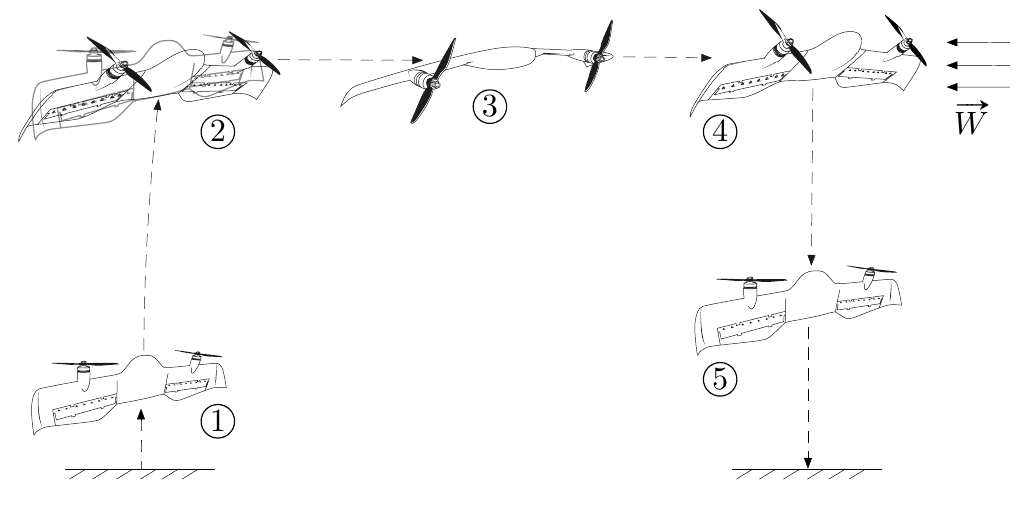
\includegraphics[width=0.8\columnwidth]{figures/darko_transition.png}
        \caption{Phases de vol d'un drone \textit{tailsitters}, DarkO.}
        \label{fig:darko_flight}
\end{figure}

\subsection*{Maquettes}

De nombreuses maquettes réelles ont été assemblées dans le but de réaliser des vols expérimentaux. Citons en exemples le \textit{tailsitter} à double rotor appelé «~T-Wing~» \cite{Stone2002PreliminaryDO, TWing2008}, le \textit{tailsitter} appelé «~MavIon~» \cite{oatao14575}, ou le «~JLion~» et le «~KH-Lion~» \cite{8003167}. Ces trois maquettes sont illustrées sur la figure \ref{fig:maquettetailsitter}.

\begin{figure}[ht!]
    \centering
    \resizebox{.9\textwidth}{!}{%
    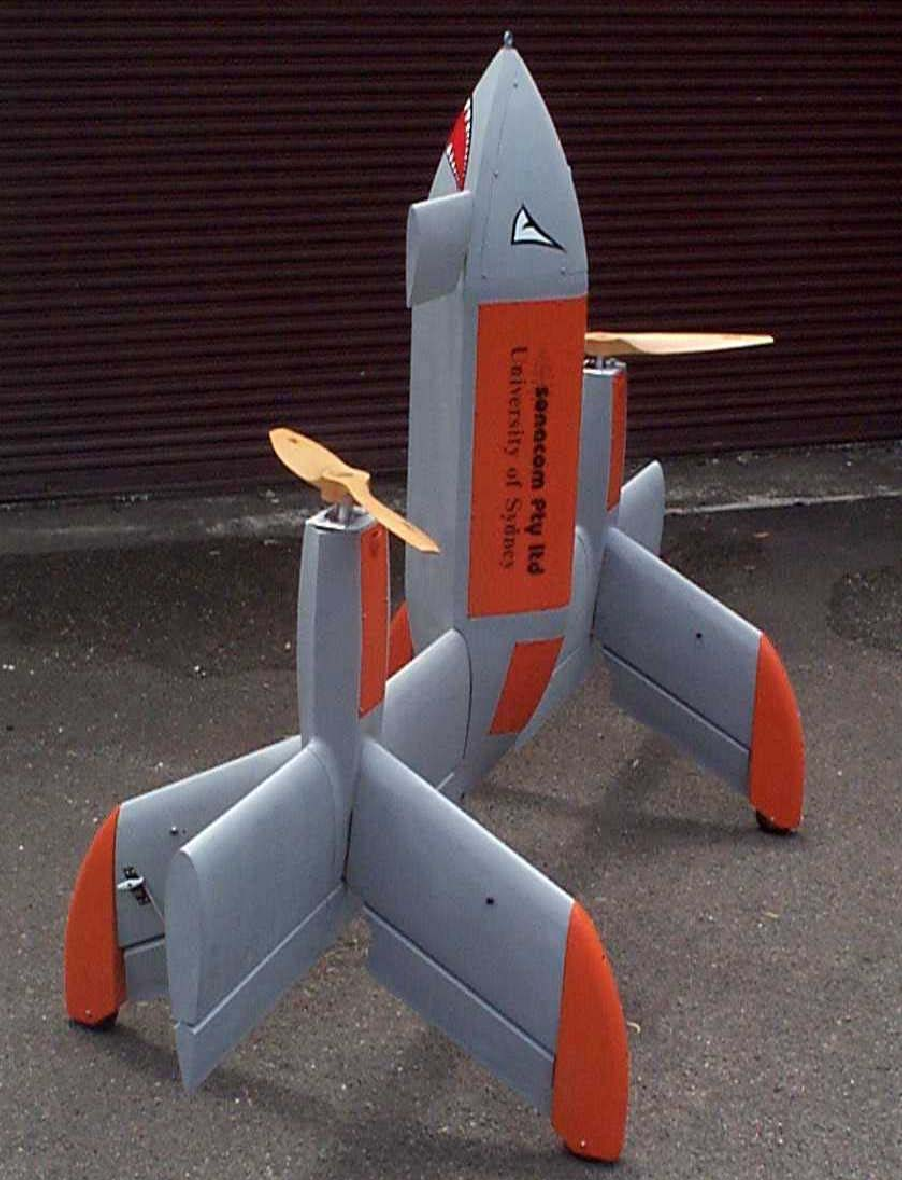
\includegraphics[height=3cm]{figures/T-Wing.png}
    \quad
    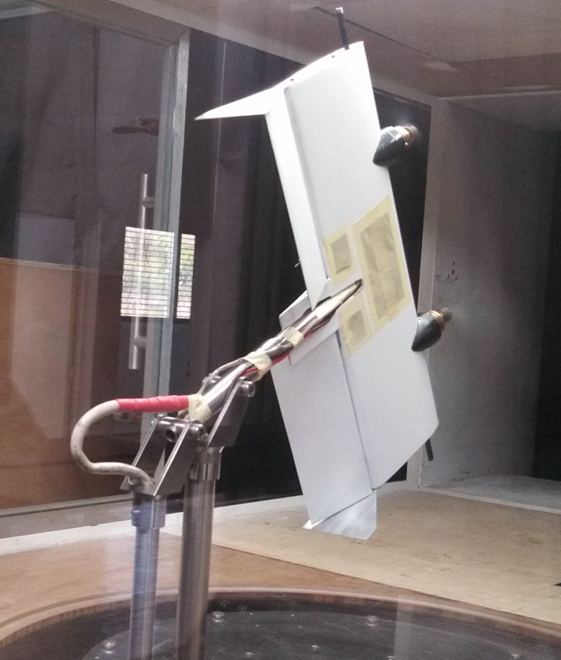
\includegraphics[height=3cm]{figures/mavionWindtunel.png}
    \quad
    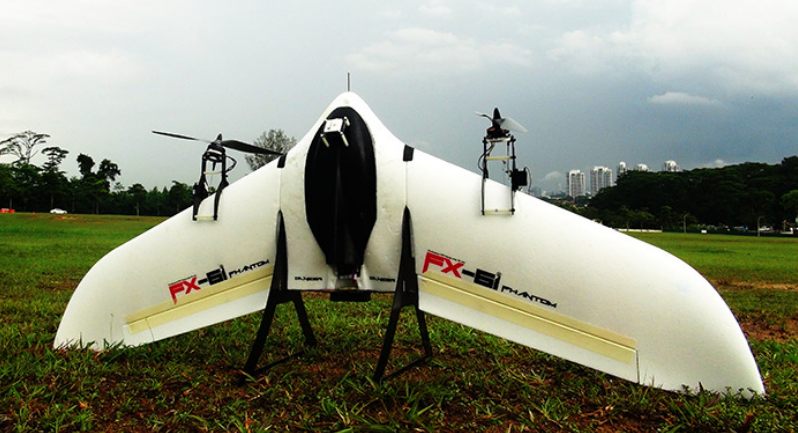
\includegraphics[height=3cm]{figures/KHlion.png}
    }
    \caption{Maquette «~T-Wing~», «~MavIon~» et «~KH-Lion~».}
    \label{fig:maquettetailsitter}
\end{figure}

Ces drones partagent une architecture similaire basée sur une aile supportant deux moteurs sur le bord d'attaque et soufflant deux élevons situés sur le bord de fuite. Cette architecture offre une plus grande robustesse que les \textit{tiltrotors}, composés de pièces mobiles (ce qui les rend plus fragiles) et d'un actionneur puissant pour faire tourner l'ensemble moteur-hélice.
La complexité inhérente à ces architectures nécessite un travail de modélisation en raison des nombreuses non-linéarités et couplages impliqués, en particulier en termes de modélisation des effets aérodynamiques. Dans ce contexte, l'interférence aérodynamique entre l'aile fixe et les rotors a été modélisée dans \cite{droandi_zanotti_gibertini_grassi_campanardi_2015, Simmons2022, aerospace5030079}, et les forces et moments d'hélice générés à des angles d'attaque élevés sont abordés dans \cite{Fernandez2023}. Cependant, ces modèles sont complexes algorithmiquement et ne sont que partiellement utilisables pour la conception des commandes. 

Un autre point important est la représentation de l'attitude du drone. Aussi, il est possible de représenter son orientation par des angles d'Euler \cite{4177650, 5415267, 8003165}, ce qui permet une compréhension intuitive. Toutefois, une singularité apparaît dans certaines phases de vol. Compte tenu de la grande manœuvrabilité, il est préférable de représenter l'attitude par un quaternion unitaire, ce qui élimine toute singularité \cite{8027691}. De nombreuses publications modélisent les effets aérodynamiques générés par les hélices en fonction de l'angle d'attaque et l'angle de dérapage \cite{Escareno07, ChiappinelliNahon2018}. 
Il est possible de choisir un autre modèle pour les interactions aérodynamiques entre les moteurs, les ailes et les élevons, comme présenté dans \cite{lustosaHal-03035938}. La technique de modélisation présentée dans \cite{lustosaHal-03035938} permet de disposer d'un modèle global couvrant l'ensemble de l'enveloppe de vol, grâce à ce que l'on appelle l'approche $\Phi$-théorie. Bien que cette dernière ne permette pas de prédire la chute brutale de la force de portance avec un angle d'attaque croissant (qui est causée par un flux d'air turbulent) \cite{tal2022global}, elle permet de représenter le drone avec suffisamment de précision pour capturer le comportement lors de manœuvres agressives. 



% Actuellement, nous pouvons mentionner deux types d'architectures de commande ayant fonctionné sur ce tailsitter. La première est basée sur une inversion incrémentale non-linéaire de la dynamique du drone (\textit{Incremental Non-linear Dynamic Inversion}, INDI) \nomenclature[]{\(INDI\)}{Inversion incrémentale non-linéaire  (\textit{Incremental Non-linear Dynamic Inversion})} et la seconde est basée sur une technique sans modèle (\textit{Model free control}, MFC). \nomenclature[]{\(MFC\)}{Commande sans modèle (\textit{Model free control})}

Les deux architectures sur lesquelles se sont concentrées nos recherches sont celles de DarkO, un \textit{tailsitters} et de Colibri, un \textit{freewings} basé sur une aile inspirée de DarkO, en rotation libre autour d'un fuselage qui sera maintenu horizontal.


\section*{Question de recherche}

Comme expliqué précédemment, lors des phases de décollage et d'atterrissage, le drone est vertical (voir figure~\ref{fig:darko_flight}), ce qui engendre une grande sensibilité aux perturbations. Il semble pertinent de concentrer nos travaux sur l'étude de la robustesse des drones convertibles face au vent.
Notre travail se focalise sur la recherche d'un contrôleur de vol unifié, pour une architecture de drone fortement non-linéaire et couplée, sur l'intégralité du domaine de vol, en environnement perturbé.

\section*{Objectifs fixés pour la thèse}
Les objectifs fixés sont pluriels : il s'agira d'étudier le comportement d'un drone \textit{tailsitters} en environnement perturbé en présence de saturation des actionneurs pouvant engendrer des cycles limites. Nous utiliserons la linéarisation pour extraire la dynamique du drone autour de l'ensemble des points d'équilibre. Nous étudierons la précision des linéarisations face aux nombreuses non-linéarités du modèle. 

De nos linéarisations, de notre compréhension du fonctionnement du drone et des limites analysées, il s'agira de proposer des architectures de commande basées modèle pour un drone \textit{tailsitters} permettant d'assurer une robustesse aux perturbations de vent. L'intérêt d'une architecture basée modèle est la possibilité de certification de ce type d'architecture. 

Pour finir, nous souhaitons utiliser des capteurs pour mesurer les perturbations en avance de phase pour les rejeter (sonde 5 trous, micro, Pitot, etc.). La connaissance d'une perturbation en amont de son impact sur le drone peut être un point clé dans la diminution de son impact. La mesure associée à un modèle peut être un moyen d'agir en anticipation plutôt qu'en réaction. Une action en anticipation pourrait se traduire par une modification de l'état du drone avant l'arrivée de la perturbation pour en minimiser son impact. À l'inverse qu'une action en réaction est une gestion de la perturbation suite à une modification de l'équilibre du drone (déplacement ou modification de son orientation) qui intervient après que la perturbation ait impacté le drone.  

Au vu des contraintes des \textit{tailsitters}, l'installation de capteurs de mesure de vent implique le développement d'une nouvelle architecture permettant l'installation d'un capteur capable de saisir les perturbations sur l'intégralité du domaine de vol.


\section*{Plan et contribution}
Notre exposé commencera par une description générale des architectures de drone convertible (Chapitre~\ref{chap:generalites}), avec une présentation des avantages et des inconvénients ainsi que leur mode de fonctionnement. Une description générale de la modélisation, de l'actionnement et des lois de commande proposée sur les \textit{tailsitters} et les \textit{freewings} introduira nos propos sur ces architectures.

Le chapitre \ref{chap:model} détaillera le modèle non-linéaire d'un drone \textit{tailsitters}, DarkO, à partir des travaux de \cite{lustosaHal-03035938} et de \cite{olszaneckibarthHal-02542982}. Nous proposons un modèle simplifié pour les basses vitesses, ainsi que le détail des équilibres stationnaires en présence ou non de vent. De ces équilibres, nous présenterons la dynamique linéarisée du drone paramétrée par deux scalaires, le vent horizontal et vertical. Ce modèle étant le point de départ de chacun de nos travaux, il se retrouve expliqué dans \cite[Chapitre 2]{sansouStage} et \cite[Section II]{sansouECC} dans la condition de vent nulle, dans \cite[Section 2]{SANSOUACA} avec des conditions de vent non nulle et dans \cite[Section II]{sansouTCST} sous sa forme la plus complète.

Le chapitre \ref{chap:hybrid} fera l'objet d'une proposition de loi de commande hybride permettant d'augmenter le domaine de stabilité d'une loi linéaire avec une loi de commande non-linéaire basée sur une direction de zéro moment. Ces travaux ont été publiés dans  \cite{sansouStage} et \cite{sansouECC}.

Le chapitre \ref{chap:3DOF} permettra de décrire une maquette expérimentale utilisée pour évaluer les performances d'une loi de commande basée sur une architecture proportionnelle dérivative. Cette loi est un retour de sortie permettant de stabiliser une position stationnaire en présence de vent. Cette maquette restreint les degrés de liberté classiques d'un drone pour se concentrer sur la réjection de perturbation de vent, grâce à un changement d'incidence de la maquette. La description de la loi de commande, son optimisation et les résultats sont disponibles dans \cite{SANSOUACA}.

Le chapitre \ref{chap:LMI} propose une méthode d'obtention des gains de la boucle fermée différente basée sur les inégalités linéaires matricielles et la théorie de Lyapunov. L'ensemble de l'optimisation sera réalisé à l'aide de la dynamique linéarisé du drone autour de la condition de vent nulle. Ce contrôleur sera testé sur une maquette à six degrés de liberté en environnement contrôlé.

Le chapitre \ref{chap:6DOF} étendra le contrôleur proposé dans le chapitre \ref{chap:3DOF} pour stabiliser la dynamique complète d'un drone \textit{tailsitter}. La méthode d'obtention des gains du contrôleur est basée sur un algorithme itératif permettant de maintenir la complexité algorithmique, tout en identifiant les conditions de vol critiques. Les travaux ont été publiés dans \cite{sansouTCST}.

Le chapitre \ref{chap:colibri} propose une nouvelle architecture de \textit{freewing}. Cette dernière est inspirée d'un \textit{tailsitter} sur lequel on adjoint un fuselage pendulaire en rotation libre de manière à le maintenir horizontal dans toutes les configurations de vol. Nos travaux se sont concentrés sur l'obtention d'un modèle de simulation basé sur une dynamique multicorps. Des résultats de simulation et expérimentaux ont été proposés, basés sur un contrôle non-linéaire et publiés dans \cite{sansouICUAS}.





\chapter{Objectifs de commande}
\minitoc
\label{chap:objectif}

\section{Contexte opérationnel}
Tout l'intérêt des drones est leurs capacités à se maintenir stabilisé sans intervention humaine. Ainsi, les opérateurs peuvent se concentrer sur la mission, sans devoir consacrer une grande attention au pilotage du drone. 

Les nombreux progrès dans les systèmes d'estimation état permettent de connaitre précisément l'orientation et la position des drones pour assurer la stabilisation, le guidage et la navigation. Les progrès sont lié à l'amélioration continue des capteurs, notamment des centrales inertielles (Inertial measurement Units, IMU), \nomenclature[]{\(IMU\)}{Centrales inertielles (\textit{Inertial measurement Units})} constitué d'un accéléromètre, d'un gyroscope et d'un magnétomètre. La Table \ref{tab:autopilote_ev} montre l'évolution des vitesses des microcontrôleurs (Microcontroller Unit, MCU) \nomenclature[]{\(MCU\)}{Microcontrôleurs (\textit{Inertial measurement Units})} embarqué sur les autopilotes et de la réduction du bruit des capteurs inertiel.
\begin{table}[ht]
    \centering
    \begin{tabular}{|c|c|c|c|c|c|}
        \hline
        Génération & Année & MCU & Vitesse & Capteur  & Bruit RMS \\
        \hline \hline
        \href{https://wiki.paparazziuav.org/wiki/Apogee/v1.00}{Apogee}  & 2013 & STM32F4 & 168 MHz & MPU-9150 & \begin{tabular}{ccc} Gyro : 0.06 dps \\
        Accel: 4 mg  \end{tabular}  \\
        \hline
        \href{https://wiki.paparazziuav.org/wiki/Chimera/v1.00}{Chimera} & 2016 & STM32F7 & 216 MHz &  MPU-9250 & \begin{tabular}{ccc} Gyro : 0.1  dps \\
        Accel: 8 mg  \end{tabular}\\
        \hline
        \href{https://wiki.paparazziuav.org/wiki/Tawaki/v1.10}{Tawaki 1} &2019 &  STM32F7 & 216 MHz  & ICM-20600 & \begin{tabular}{ccc} Gyro : 0.04 dps \\
        Accel: 1 mg  \end{tabular}\\
        \hline
        \href{https://wiki.paparazziuav.org/wiki/Tawaki/v2.01}{Tawaki 2} &2023 &  STM32H7 & 480 MHz & ICM-42688-P & \begin{tabular}{ccc} Gyro : 0.028 dps \\
        Accel: 0.70 mg  \end{tabular} \\
        \hline
    \end{tabular}
    \caption{Évolution des autopilotes paparazzi sur dix ans.}
    \label{tab:autopilote_ev}
\end{table}

Sur une période de dix ans, nous pouvons observer que les microcontrôleurs ont doublé leurs vitesses d'exécution, que les fabricants ont divisé par deux le bruit moyen sur les gyroscopes et par quatre le bruit moyen des accéléromètres.
Ces évolutions continues permettent une amélioration de l'estimation du drone utilisé pour la stabilisation. Il en résulte une stabilité accrue et de nouvelle possibilité pour la commande des drones.


\section{Contexte de la thèse}
De nombreux travaux ont été mener sur les \textit{tailsitters}, avec l'objectif de couvrir l'intégralité du domaine de vol. Ce dernier est constitué de trois phases, le stationnaire, la transition et le vol d'avancement. Chaque phase possède des contraintes  

vol complet 
methode sans modèles 




\todo{rejet de perturbation, model based control}

\section{Perturbations}

\section{Résumée}
\chapter{Modélisation d'un drone convertible : DarkO}
\minitoc
\label{chap:model}

\section{Modèle du drone DarkO}
\label{sec:model}
DarkO, drone conçu et développé à l'École Nationale de l'Aviation Civile (ENAC) de Toulouse (France), est un exemple clair de drone convertible avec une architecture dite \textit{tailsitter}.
DarkO est assemblé à partir de plusieurs pièces d'Onyx imprimées en 3D (un matériau très robuste composé de fibres de carbone omnidirectionnelles). Toutes les pièces sont emboîtées sur un seul axe, de sorte que le drone puisse facilement être démonté pour remplacer des pièces ou accéder à l'électronique embarquée. 

L'autopilote embarqué est une carte Apogee~\footnote{\url{https://wiki.paparazziuav.org/wiki/Apogee/v1.00}} fabriquée à l'ENAC, voir Fig. \ref{fig:apogee}. 


\begin{figure}[ht!]
    \centering
        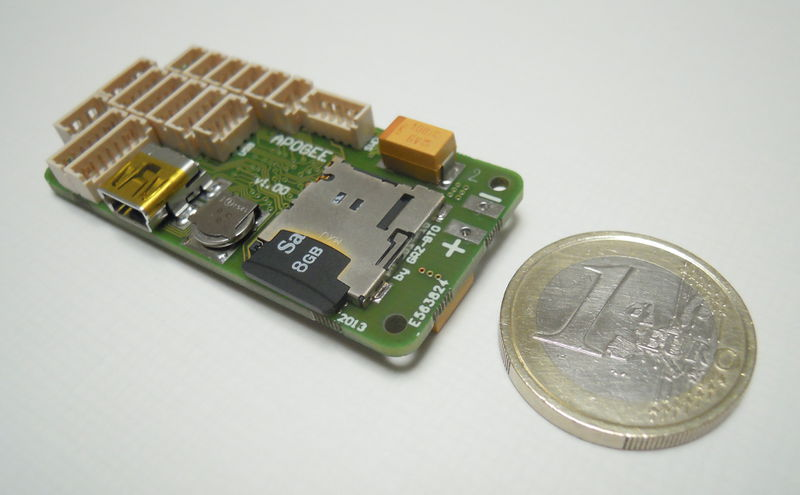
\includegraphics[width=0.8\columnwidth]{figures/800px-Apogee_v100_top_1E.jpeg}
        \caption{Vue de dessus d'un autopilote Apogee v1.00.}
        \label{fig:apogee}
\end{figure}

L'autopilote offre la possibilité d'enregistrer les données de bord sur une carte mémoire SD, à la fréquence de contrôle de 500 Hz, ce qui permet un post-traitement efficace des données acquises. Le protocole de communication utilisé entre l'autopilote et les contrôleurs électroniques de vitesse (ESC) est le Dshot 600. Les ESC sont des AIKON AK32 35A \todo{trouver un synonyme} flasher avec un firmware AM32. La communication sol-bord est réalisée via un canal bidirectionnel basé sur des modules XBee-PRO S1.

\nomenclature[]{\(ESC\)}{Contrôleurs électroniques de vitesse (\textit{Electronic Speed Controller})}



Les actionneurs de DarkO peuvent être décomposés en deux catégories. La première est composée de deux hélices (T-Motor T5147) placées symétriquement à l'avant de l'aile (illustrées en \textbf{noir} dans la Fig. \ref{fig:darko2}) et alimentées par deux moteurs électriques (T-Motor F30 2300kv) générant une traction selon l'axe $x_{b}$. La seconde catégorie est relative aux actionneurs aérodynamiques. Ainsi, le drone possède deux élevons, placés à l'arrière de l'aile (illustrés en \textcolor{cyan}{bleu} dans la Fig. \ref{fig:darko2}), agissant en tant que surfaces de contrôle. Les élevons génèrent des forces et des moments en modifiant leur incidence relativement au flux d'air dans lequel ils sont placés. Ce flux d'air peut être généré par le vent relatif (lié à la vitesse du drone), le vent extérieur, mais aussi par le souffle des hélices. Les élevons sont commandés par deux servomoteurs MKS DS65K.

\begin{figure}[ht!]
    \centering
    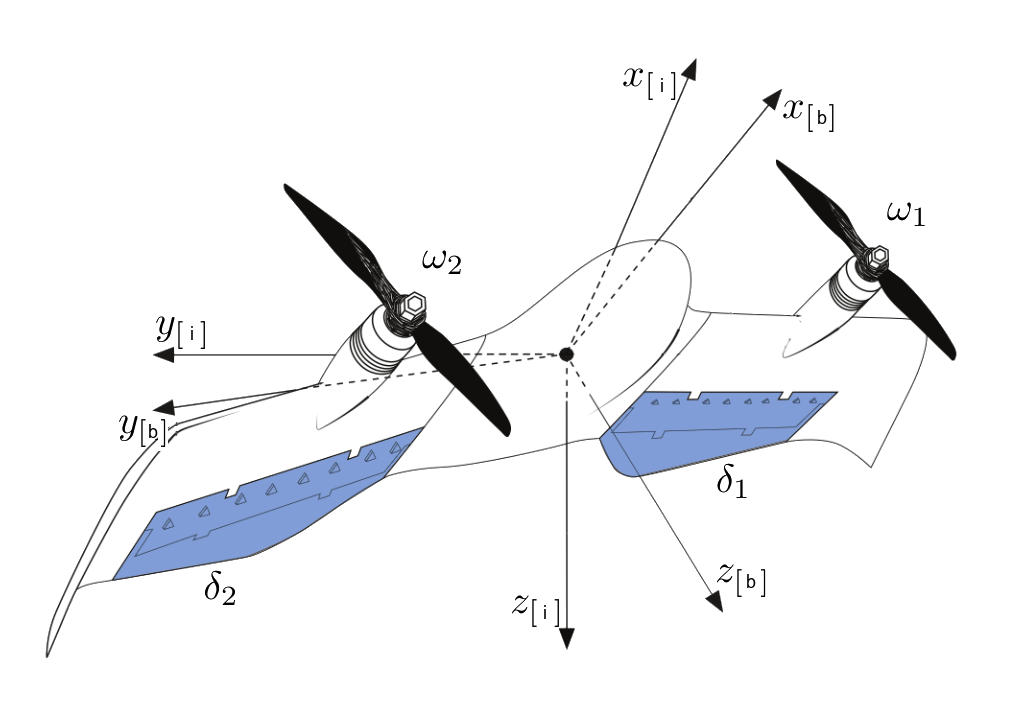
\includegraphics[width=0.8\columnwidth]{figures/darko.png}
    \caption{Repère de référence de DarkO avec une représentation schématique des actionneurs.}
    \label{fig:darko2}
\end{figure}

La figure \ref{fig:darko2} montre le modèle de DarkO, ainsi qu'un repère de référence inertiel \textit{North, east, down} (NED) \nomenclature[]{\(NED\)}{Nord Est Bas (\textit{North, East, Down})} (ou repère terrestre) ``$\text{i}$'' lié à la surface de la Terre, et un repère corps `$\text{b}$'' attaché au drone, avec $x_{\text{b}}$ correspondant à l'axe de roulis (l'axe des hélices dans le plan $z_{ \text{b} } = 0$), $y_{\text{b}}$ l'axe de tangage (la direction des ailes), $z_{\text{b}}$ l'axe de lacet. En utilisant la même notation que dans \cite{lustosaHal-03035938}, le couple hélice/élévateur gauche et droit sont désignés par les indices $i=1$ (gauche) et $i=2$ (droite). La convention de signe sera définie comme positive pour les positions des élevons $\delta_{1}$, $\delta_{2}$ lorsqu'ils créent un moment à cabrer avec les hélices tournant dans des directions opposées avec des vitesses angulaires $\omega_{1} > 0$ et $\omega_{2} < 0$, respectivement.

\begin{table}[ht]
    \centering
      \begin{tabular}{|l|c|c|}
        \hline
        \multicolumn{1}{|c|}{Paramètres et coefficients} & Valeurs & Unités \\
        \hline
        $m$ (Masse du drone)  & 0.519 & \SI{}{\kilogram} \\
        \hline
        $b$ (Envergure)  & 0.542 & \SI{}{\meter} \\
        \hline
        $c$ (Corde aérodynamique)  & 0.13 & \SI{}{\meter} \\
        \hline
        $\boldsymbol{B}=\diag(b,c,b)$ & $\!\!\diag(0.542, 0.13, 0.542)$ \!\! & \SI{}{\meter}\\
        \hline
        $S$ (Surface de l'aile) & 0.026936 & \SI{}{\square\meter}\\
        \hline
        $S_{\text{wet}}$ (Surface soufflée) & 0.0180 & \SI{}{\square\meter}\\
        \hline
        $S_{\text{p}}$ (Surface des hélices) & 0.0127 & \SI{}{\square\meter}\\
        \hline
        $\boldsymbol{J}=\diag(J_{x},J_{y},J_{z})$ & \!\! $\diag(0.0067,0.0012,0.0082)$\!\! & \SI{}{\kilogram\square\meter}\\
        \hline
        $k_{\text{f}}$ (Poussée des hélices) & 1.7800e-8 & \SI{}{\kilogram\meter}\\
        \hline
        $k_{\text{m}}$(Moment des hélices) & 2.1065e-10 & \SI{}{\kilogram\square\meter}\\
        \hline
        $p_{x}$ (Position en $x$ des hélices) & 0.065 & \SI{}{\meter}\\
        \hline
        $p_{y}$ (Position en $y$  des hélices) & 0.162 & \SI{}{\meter}\\
        \hline
        $a_{y}$ (Position en $y$ de la portance) & 0.1504 & \SI{}{\meter}\\
        \hline
        $\xi_{\text{f}}$ (Portance des élevons) & 0.2 & --\\
        \hline
        $\xi_{\text{m}}$ (Moment des élevons) & 1.4 & --\\
        \hline
        $\rho$ (Densité de l'air) & 1.225 & \SI{}{\kilogram\per\cubic\meter}\\
        \hline
        $C_{\text{d}}$ (Trainé) & 0.1644 & --\\
        \hline
        $C_{y}$ (Latéral) & 0 & --\\
        \hline
         $C_{\ell}$ (Portance) & 5.4001 & --\\
        \hline
        $\Delta_{\text{r}}$ (Centrage du drone) & -0.0145 & \SI{}{\meter}\\
        \hline
      \end{tabular}
      \caption{Paramètres numériques identifiés du modèle DarkO.}
      \label{tab:pars}
\end{table}

\subsection{Modèle non-linéaire complet}

En exploitant la modélisation présentée dans \cite{lustosaHal-03035938} et \cite{olszaneckibarthHal-02542982}, un modèle précis de la dynamique de DarkO décrit la position $\boldsymbol{p} \in \real^3$ du centre de gravité et sa vitesse $\boldsymbol{v} = \dot{\boldsymbol{p}} \in \real^3$, son orientation, bien représentée par un quaternion $\boldsymbol{q} \in {\mathbb S}^3:=\{ \boldsymbol{q} \in \real^4 : |\boldsymbol{q}| = 1\}$, et de sa vitesse angulaire $\boldsymbol{\omega}_{\text{b}}$, représentée dans le repère du corps, qui satisfait $\boldsymbol{\dot q} = \frac{1}{2}\boldsymbol{q} \otimes \smallmat{0 \\ \boldsymbol{\omega}_{{\text{b}}}}$, où $\otimes$ représente le produit hamiltonien (voir \cite{lustosaHal-03035938,olszaneckibarthHal-02542982} ou le tutoriel \cite{hamel_minhduc} pour plus de détails).
\todo{produit hamiltonien}
En choisissant l'état global comme $\boldsymbol{x}:=(\boldsymbol{p},~ \boldsymbol{v},~ \boldsymbol{q},~ \boldsymbol{\omega}_{\text{b}})$, le modèle mathématique, dérivé dans \cite{lustosaHal-03035938}, dépend d'un ensemble de paramètres énumérés dans le tableau \ref{tab:pars}, où nous indiquons également la valeur obtenue à partir d'une identification du système \cite{sansouStage}. Le modèle dynamique peut être écrit comme ci-dessous :

\begin{subequations}\label{eq:dyna_orig}
    \begin{empheq}[left=\empheqlbrace]{alignat=2}
           \boldsymbol{\dot p} & &= & \boldsymbol{v} \label{eq:dyna_orig_a}\\
          \label{eq:dyna_orig_b}
          m\boldsymbol{\dot v} &&=& - m\boldsymbol{g} +  \boldsymbol{R}(\boldsymbol{q})\boldsymbol{F}_{\text{b}},\\
          \boldsymbol{\dot q} &&=& \frac{1}{2}\boldsymbol{q} \otimes \boldsymbol{\omega_{b}} \label{eq:dyna_orig_c}\\
          \label{eq:dyna_orig_d}
          \boldsymbol{J} \boldsymbol{\dot \omega_{\text{b}}} &&= &  - \skewsym{\boldsymbol{\omega}_{\text{b}}}\boldsymbol{J}\boldsymbol{\omega}_{\text{b}} + \boldsymbol{M}_{\text{b}},
    \end{empheq}
  \end{subequations}
  où $\boldsymbol{g}:=\smallmat{0 & 0& 9.81}^\top$ désigne le vecteur de gravité, $m\in \real$ est la masse, $\boldsymbol{J}\in \real^{3\times 3}$ est le moment d'inertie diagonal (voir Tableau~\ref{tab:pars}) et en partitionnant le quaternion $\boldsymbol{q} \in {\mathbb S}^3$ comme $\boldsymbol{q} := \left[ \eta ~ \boldsymbol{\epsilon}^\top \right]^\top$, la matrice de rotation correspondante est $\boldsymbol{R}(\boldsymbol{q}) \in SO(3): = \{\boldsymbol{R}\in \real^{3\times 3}: \; \boldsymbol{R}^\top \boldsymbol{R} = \mathbb{I}_{3}, \det (\boldsymbol{R})=1\}$ est défini comme (voir \cite{hamel_minhduc})
\begin{align}
    \label{eq:matrix_rot}
    \boldsymbol{R}(\boldsymbol{q}) := \mathbb{I}_{3} +2\eta \skewsym{\boldsymbol{\epsilon}} + 2\skewsym{\boldsymbol{\epsilon}}^{2}.
\end{align}


D'après \cite{lustosaHal-03035938}, le vecteur de force $\boldsymbol{F}_{\text{b}}$ et le vecteur de moment $\boldsymbol{M}_{\text{b}}$ dans \eqref{eq:dyna_orig} dépendent  (i) de l'état du système $\boldsymbol{x}$, (ii) de la perturbation $\boldsymbol{w} \in \real^3$, représentant la vitesse du vent dans le référentiel inertiel, et (iii) de la commande des actionneurs (voir Figure~\ref{fig:darko2}), comprenant la vitesse de rotation des deux hélices $\omega_1, \omega_2 \in \real$ et la déflexion des élevons $\delta_1, \delta_2\in \real$.
Considérons d'abord l'effet des commandes des actionneurs. Chaque hélice génère une poussée $\boldsymbol{T}_i$ orientée dans la direction $x$ du repère corps et un moment $\boldsymbol{N}_i$ selon le même axe :
\begin{align}
\label{eq:thrust}
\boldsymbol{T}_{i} \!:=\! \begin{bmatrix} \tau_{i} \\ 0 \\ 0 \end{bmatrix} \!:=\!
\begin{bmatrix} k_{\text{f}}\omega_{i}^{2} \\ 0 \\ 0 \end{bmatrix}\! , \;
\boldsymbol{N}_{i} \!:=\! (-1)^{i}  \frac{k_{\text{m}} }{k_{\text{f}}}\boldsymbol{T}_{i}, \quad i=1,2 .
\end{align} 

La position de chaque élevon $\delta_i \in \real$ est assignée par un servomoteur qui impose un niveau d'efficacité (en termes de déviation du courant d'air) quantifié par deux matrices antisymétriques :
\begin{align}
\label{eq:elevons_efficiency}
    \boldsymbol{\Delta}^{\text{f}}_{i} \!:=\! \begin{bmatrix} 0 & 0 & \xi_{\text{f}}\delta_{i} \\ 0 & 0 & 0 \\ -\xi_{\text{f}}\delta_{i} & 0 & 0 \end{bmatrix}\! ,\;
    \boldsymbol{\Delta}^{\text{m}}_{i} \!:=\! \begin{bmatrix} 0 & 0 & \xi_{\text{m}}\delta_{i} \\ 0 & 0 & 0 \\ -\xi_{\text{m}}\delta_{i} & 0 & 0 \end{bmatrix} \!, \quad i=1,2.
\end{align}
 Les paramètres constants $k_{\text{f}}$, $k_{\text{m}}$, $\xi_{\text{f}}$, $\xi_{\text{m}}$ apparaissant dans \eqref{eq:thrust} et \eqref{eq:elevons_efficiency} sont listés dans la Table~\ref{tab:pars}.\\
Avec les quantités ci-dessus, nous pouvons réarranger la dynamique donnée dans le tableau suivant \cite[eqns (97),~(98)]{lustosaHal-03035938} (voir aussi \cite{sansouStage}) et exprimer $\boldsymbol{F}_{\text{b}}$ et $\boldsymbol{M}_{\text{b}}$ dans \eqref{eq:dyna_orig} comme
%
\begin{align}
\nonumber
    \boldsymbol{F}_{\text{b}} :={}&  \boldsymbol{T}_{1} + \boldsymbol{T}_{2} + \frac{S_{\text{wet}}}{4S_{\text{p}}} \boldsymbol{\Phi}^{\text{(fv)}} \Big( (\boldsymbol{\Delta}^{\text{f}}_1 - \mathbb{I}_{3} ) \boldsymbol{T}_{1} + ( \boldsymbol{\Delta}^{\text{f}}_2 - \mathbb{I}_{3}) \boldsymbol{T}_{2}\Big) \\ 
     \label{eq:Fb}
    &+ \frac{1}{4} \rho S  \boldsymbol{\Phi}^{\text{(fv)}} \Big(\boldsymbol{\Delta}^{\text{f}}_1+ \boldsymbol{\Delta}^{\text{f}}_2 - 2 \mathbb{I}_{3} \Big) \lVert \boldsymbol{v_{\text{b}}} \rVert \boldsymbol{v_{\text{b}}}\\
    \nonumber
    &+ \frac{1}{4} \rho S \boldsymbol{\Phi}^{\text{(mv)}} \Big(\boldsymbol{\Delta}^{\text{f}}_1 + \boldsymbol{\Delta}^{\text{f}}_2 - 2\mathbb{I}_{3}\Big) \boldsymbol{B} \lVert \boldsymbol{v_{\text{b}}} \rVert  \boldsymbol{\omega}_{\text{b}}, 
\end{align}
\begin{align} 
\label{eq:Mb}
 \boldsymbol{M}_{\text{b}} :&=\boldsymbol{N}_{1} + \boldsymbol{N}_{2} + \skewsym{\smallm{p_x\\ p_y\\ 0}} \boldsymbol{T}_{1} + \skewsym{\smallm{p_x\\ - p_y\\ 0}} \boldsymbol{T}_{2}\\
    \nonumber
  &- \frac{S_{\text{wet}}}{4S_{\text{p}}} \bigg( \boldsymbol{B} \boldsymbol{\Phi}^{\text{(mv)}} (\boldsymbol{\Delta}^{\text{m}}_1- \mathbb{I}_{3} ) + \skewsym{\smallm{0 \\ a_y \\ 0}} \boldsymbol{\Phi}^{\text{(fv)}} (\boldsymbol{\Delta}^{\text{m}}_1 +\mathbb{I}_{3} ) \bigg) \boldsymbol{T}_{1} \\
    \nonumber
  & - \frac{S_{\text{wet}}}{4S_{\text{p}}} \bigg( \boldsymbol{B} \boldsymbol{\Phi}^{\text{(mv)}} (\boldsymbol{\Delta}^{\text{m}}_2 - \mathbb{I}_{3} ) +  \skewsym{\smallm{0 \\ - a_y \\ 0}} \boldsymbol{\Phi}^{\text{(fv)}} (\boldsymbol{\Delta}^{\text{m}}_2 + \mathbb{I}_{3}) \bigg) \boldsymbol{T}_{2} \\
    \nonumber
  & + \frac{1}{4} \rho S  \bigg( \Big(\skewsym{\smallm{0 \\ a_y \\ 0}} \!\!\! \boldsymbol{\Phi}^{\text{(fv)}}  + \boldsymbol{B} \boldsymbol{\Phi}^{\text{(mv)}} \Big) \boldsymbol{\Delta}^{\text{m}}_1 \\
    \nonumber
  &  + \Big( \skewsym{\smallm{0 \\ - a_y \\ 0}} \!\!\! \boldsymbol{\Phi}^{\text{(fv)}} + \boldsymbol{B} \boldsymbol{\Phi}^{\text{(mv)}}  \Big) \boldsymbol{\Delta}^{\text{m}}_2 - 2 \boldsymbol{B} \boldsymbol{\Phi}^{\text{(mv)}}  \bigg) \lVert \boldsymbol{v_{\text{b}}} \rVert \boldsymbol{v_{\text{b}}} \\
    \nonumber
  & +\frac{1}{4} \rho S \bigg(\!\! \Big(\!\! \skewsym{\!\smallm{0 \\ a_y \\ 0}\!}\!\!\! \boldsymbol{\Phi}^{\text{(mv)}} \! + \! \boldsymbol{B} \boldsymbol{\Phi}^{\text{(m$\omega$)}} \Big) \boldsymbol{\Delta}^{\text{m}}_1 \\
    \nonumber
  & +  \Big(\!\! \skewsym{\!\smallm{0 \\ - a_y \\ 0}\!} \!\!\! \boldsymbol{\Phi}^{\text{(mv)}} \! + \! \boldsymbol{B} \boldsymbol{\Phi}^{\text{(m$\omega$)}}  \Big) \boldsymbol{\Delta}^{\text{m}}_2 - 2 \boldsymbol{B} \boldsymbol{\Phi}^{\text{(m$\omega$)}}\!  \bigg)\!  \boldsymbol{B}  \lVert \boldsymbol{v_{\text{b}}} \rVert  \boldsymbol{\omega}_{\text{b}} ,
\end{align}
où $\boldsymbol{v}_{\text{b}} := \boldsymbol{R}^\top(\boldsymbol{q}) (\boldsymbol{v}-\boldsymbol{w})$ représente la vitesse de l'air vu par le drone exprimé dans le repère du corps. Dans \cite{lustosaHal-03035938}, la valeur $\lVert \boldsymbol{v_{\text{b}}} \rVert$ apparaissant dans les expressions de  $\boldsymbol{F}_{\text{b}}$ et $\boldsymbol{M}_{\text{b}}$ est remplacé par la valeur $\eta = \sqrt{\lVert \boldsymbol{v_{\text{b}}} \rVert^{2} + \mu c^{2} \lVert \boldsymbol{\omega}_{\text{b}} \rVert^{2}}$, avec $\mu \in \real$ étant un paramètre lié à l'identification du modèle. Toutefois, dans le cas de DarkO, l'identification fournit $\mu = 0$ \cite{sansouStage}. Ainsi, nous présentons ici une description simplifiée. La matrice des coefficients aérodynamiques constants 
$\boldsymbol{\Phi}:= \begin{bmatrix} \boldsymbol{\Phi}^{\text{(fv)}} & {\boldsymbol{\Phi}^{\text{(mv)}}}^\top \\ \boldsymbol{\Phi}^{\text{(mv)}} & \boldsymbol{\Phi}^{\text{(m$\omega$)}} \end{bmatrix} \in \real^{6 \times 6}$, est défini dans \cite[eqs. (6)--(9)]{olszaneckibarthHal-02542982} comme $ \boldsymbol{\Phi}^{\text{(fv)}} \!:=\! \diag(C_{\text{d}},C_{y}, C_{\ell})$ et
\begin{align*}
&\left[ \begin{array}{c|c}
    \boldsymbol{\Phi}^{\text{(mv)}}  &  \boldsymbol{\Phi}^{\text{(m$\omega$)}} 
\end{array}\right] :=\\ 
&\left[ \begin{array}{ccc|ccc}
    0 & 0 & 0    &                                          0.1396 & 0 & 0.0573 \\
    0 & 0 & \!\!\!\!\! -\frac{\Delta_{\text{r}}}{c}C_{\ell} &    0 &  0.6358  & 0 \\
    0 & 0 & 0 &     0.0405 & 0 & 0.0019 
\end{array}\right],
\end{align*}
les valeurs numériques des constantes figurant dans le tableau \ref{tab:pars} (ces valeurs numériques n'ont pas été indiquées dans \cite{lustosaHal-03035938} et \cite{olszaneckibarthHal-02542982} et sont données ici pour permettre de reproduire les résultats de nos simulations). 


\subsection{Modèle non linéaire simplifiée à basse vitesse}
\label{sec:model_NL_simp}

Dans la mesure où nous allons nous intéresser au maintien du drone en stationnaire, c'est-à-dire avec une vitesse du drone faible, nous pouvons simplifier la dynamique \eqref{eq:dyna_orig} en négligeant les effets aérodynamiques quadratiques dûs à la vitesse $\boldsymbol{v_{\text{b}}}$ et à la vitesse angulaire $\boldsymbol{\omega}_{\text{b}}$ dans \eqref{eq:Fb} et \eqref{eq:Mb}. 
Nous définissons le vecteur de commande :
\begin{align}
\label{eq:vector_u}
    \boldsymbol{u} := \begin{bmatrix}\tau_{1}  \!&\! \tau_{2}  \!&\! \delta_{1} \!&\! \delta_{2} \end{bmatrix}^\top,
\end{align}
lequel permet d'obtenir le modèle basse vitesse comportant les effets majeurs non-linéaires du vent :
\begin{subequations}\label{eq:dyna_simp}
    \begin{alignat}{3}
    &\boldsymbol{\dot p} = \boldsymbol{v}, \label{eq:dyna1}\\
       & m\boldsymbol{\dot v} =\! \shortminus m\boldsymbol{g} \!+ \! \boldsymbol{R} (\boldsymbol{q}) \!\!\left( \! \boldsymbol{M}_{\text{f}}(\boldsymbol{u}) \! + \! \boldsymbol{D}_{\text{f}}(\boldsymbol{u}) \| \boldsymbol{w} \| \boldsymbol{R}^\top \!(\boldsymbol{q}) (\boldsymbol{v} \! \shortminus \! \boldsymbol{w}) \! \right)\!,\!\! \label{eq:dyna2}\\
        &\boldsymbol{\dot q} = \frac{1}{2}\boldsymbol{q} \otimes \smallmat{0 \\ \boldsymbol{\omega}_{\text{b}}}, \label{eq:dyna3}\\
        &\boldsymbol{J} \boldsymbol{\dot \omega}_{\text{b}} = \shortminus \skewsym{\boldsymbol{\omega}_{\text{b}}}\boldsymbol{J}\boldsymbol{\omega}_{\text{b}}\! + \boldsymbol{M}_{\text{m}}(\boldsymbol{u})\! + \boldsymbol{D}_{\text{m}} (\boldsymbol{u}) \lVert \boldsymbol{w} \rVert \boldsymbol{R}^\top(\boldsymbol{q}) (\boldsymbol{v}-\boldsymbol{w}), \label{eq:dyna4}
    \end{alignat}
\end{subequations}
où les vecteurs $\boldsymbol{M}_{\text{f}}(\boldsymbol{u})$ et $ \boldsymbol{M}_{\text{m}}(\boldsymbol{u})$, et les matrices $\boldsymbol{D}_{\text{f}}(\boldsymbol{u})$ et $\boldsymbol{D}_{\text{m}} (\boldsymbol{u})$ proviennent de l'annulation des termes dépendant de la vitesse angulaire dans l'équation \eqref{eq:Fb} et \eqref{eq:Mb}. Ils peuvent être développés en 
\begin{align}
\label{eq:Mf}
    \boldsymbol{M}_{\text{f}}(\boldsymbol{u}) :&=  \boldsymbol{T}_{1} \!+\! \boldsymbol{T}_{2} \!+\! \frac{S_{\text{wet}}}{4S_{\text{p}}} \boldsymbol{\Phi}^{\text{(fv)}} \Big( (\boldsymbol{\Delta}^{\text{f}}_1 \shortminus \mathbb{I}_{3} ) \boldsymbol{T}_{1} + ( \boldsymbol{\Delta}^{\text{f}}_2 \shortminus \mathbb{I}_{3}) \boldsymbol{T}_{2}\Big) \nonumber\\
     &=\begin{bmatrix} \left(1-\frac{S_{\text{wet}}}{4S_{\text{p}}} C_{\text{d}}\right) (\tau_{1} + \tau_{2}) \\  0  \\ -\frac{S_{\text{wet}}}{4S_{\text{p}}}C_{\ell}\xi_{\text{f}} \left(\delta_{1}\tau_{1} + \delta_{2}\tau_{2}\right) \end{bmatrix},
\end{align}
\begin{align}
\nonumber
 \boldsymbol{M}_{\text{m}}(\boldsymbol{u}) :&= \boldsymbol{N}_{1} + \boldsymbol{N}_{2} + \skewsym{\smallm{p_x\\ p_y\\ 0}} \boldsymbol{T}_{1} + \skewsym{\smallm{p_x\\ -p_y\\ 0}} \boldsymbol{T}_{2}\\
 \nonumber
   &\quad \shortminus \frac{S_{\text{wet}}}{4S_{\text{p}}}\! \bigg( \boldsymbol{B} \boldsymbol{\Phi}^{\text{(mv)}} (\boldsymbol{\Delta}^{\text{m}}_1- \mathbb{I}_{3} ) \! + \! \skewsym{\smallm{0 \\ a_y \\ 0}} \!\! \boldsymbol{\Phi}^{\text{(fv)}} (\mathbb{I}_{3} + \boldsymbol{\Delta}^{\text{m}}_1 ) \bigg) \boldsymbol{T}_{1} \\
   \nonumber
   &\quad \shortminus \frac{S_{\text{wet}}}{4S_{\text{p}}} \!\bigg( \boldsymbol{B} \boldsymbol{\Phi}^{\text{(mv)}} (\boldsymbol{\Delta}^{\text{m}}_2 - \mathbb{I}_{3} ) \! + \! \skewsym{\smallm{0 \\ \!\shortminus a_y \!\\ 0}} \!\! \boldsymbol{\Phi}^{\text{(fv)}} (\mathbb{I}_{3} + \boldsymbol{\Delta}^{\text{m}}_2 ) \bigg) \boldsymbol{T}_{2} \\
   \label{eq:Mm}
    &=\begin{bmatrix} \frac{k_{\text{m}} }{k_{\text{f}}}(\tau_{1} - \tau_{2}) + \frac{S_{\text{wet}}}{4S_{\text{p}}}a_{y}C_{\ell}\xi_{\text{f}}(\delta_{1}\tau_{1} - \delta_{2}\tau_{2}) \\
   \frac{S_{\text{wet}}}{4S_{\text{p}}} \Delta_{\text{r}}C_{\ell}\xi_{\text{m}}(\delta_{1}\tau_{1} + \delta_{2}\tau_{2}) \\
   \left(p_{y}+\frac{S_{\text{wet}}}{4S_{\text{p}}} a_{y} C_{\text{d}}\right)(\tau_{1} - \tau_{2})
   \end{bmatrix},
\end{align}
\begin{align}
    \boldsymbol{D}_{\text{f}}(\boldsymbol{u}) :&=  \frac{1}{4} \rho S  \boldsymbol{\Phi}^{\text{(fv)}} \Big( \boldsymbol{\Delta}^{\text{f}}_1+  \boldsymbol{\Delta}^{\text{f}}_2 - 2 \mathbb{I}_{3} \Big)   \nonumber \\
 &= \frac{1}{4}\rho S  \begin{bmatrix}
       -2C_{\text{d}} & 0 & C_{\text{d}}\xi_{\text{f}}(\delta_{1} +\delta_{2})\\
       0 & 0 & 0\\
       -C_{\ell}\xi_{\text{f}}(\delta_{1} +\delta_{2}) & 0 & -2C_{\ell}
   \end{bmatrix}, \label{eq:df}
\end{align}
\begin{align}
    \nonumber
    \boldsymbol{D}_{\text{m}}(\boldsymbol{u}) :&= \frac{1}{4} \rho S  \bigg( \Big(\skewsym{\smallm{0 \\ a_y \\ 0}} \!\!\!  \boldsymbol{\Phi}^{\text{(fv)}}  +  \boldsymbol{B}  \boldsymbol{\Phi}^{\text{(mv)}} \Big)  \boldsymbol{\Delta}^{\text{m}}_1  \\
     &\quad  + \Big( \skewsym{\smallm{0 \\ -a_y \\ 0}} \!\!\!  \boldsymbol{\Phi}^{\text{(fv)}} +  \boldsymbol{B}  \boldsymbol{\Phi}^{\text{(mv)}}  \Big)  \boldsymbol{\Delta}^{\text{m}}_2 - 2  \boldsymbol{B}  \boldsymbol{\Phi}^{\text{(mv)}}  \bigg) \nonumber \\
     &= \frac{1}{4}\rho S  \begin{bmatrix}
              \shortminus a_{y}C_{\text{d}}\xi_{\text{m}}(\delta_{1} \!-\! \delta_{2}) \!\! & 0 & 0\\
              \Delta_{\text{r}}C_{\ell}\xi_{\text{m}}(\delta_{1} +\delta_{2})\!\! & 0 & 2\Delta_{\text{r}}C_{\ell}\\
             0 & 0 & \!\! \shortminus a_{y}C_{\ell}\xi_{\text{m}}(\delta_{1} \!-\!\delta_{2})
          \end{bmatrix},   \label{eq:dm}  
\end{align}
où l'on observe l'effet non linéaire d'un vent non nul, qui est non linéaire avec $\boldsymbol{q}$, $\lVert \boldsymbol{v}_{\text{b}} \rVert$ et $\boldsymbol{w}$. Comme dans \cite[eqn. (10)]{olszaneckibarthHal-02542982} et selon la formule de Diederich, nous obtenons $C_{\ell} = C_{\text{d}} + \frac{\pi AR}{1+\sqrt{1+\left(\frac{AR}{2}\right)^{2}}}$ où $AR = \frac{b^{2}}{S}$ est l'allongement de l'aile.
Nous observons le couplage des actionneurs $\left(\delta_{1}\tau_{1} + \delta_{2}\tau_{2}\right)$  dans les expressions des matrices $\boldsymbol{M}_{\text{f}}(\boldsymbol{u})$ et $\boldsymbol{M}_{\text{m}}(\boldsymbol{u})$.

\section{Identification des paramètres du modèle}
    Les valeurs numériques du tableau \ref{tab:pars} ont été obtenues par une campagne d'identification du modèle \cite{sansouStage}. En particulier, le coefficient $k_{\text{f}}$ a été identifié à partir de l'équation \eqref{eq:thrust}, qui relie la vitesse de rotation du moteur $\omega_{i}$ à la traction générée, à la vitesse de rotation minimale et maximale et à la constante de temps de la chaîne d'actionnement du moteur.
    \begin{figure}[ht!]
        \centerline{
        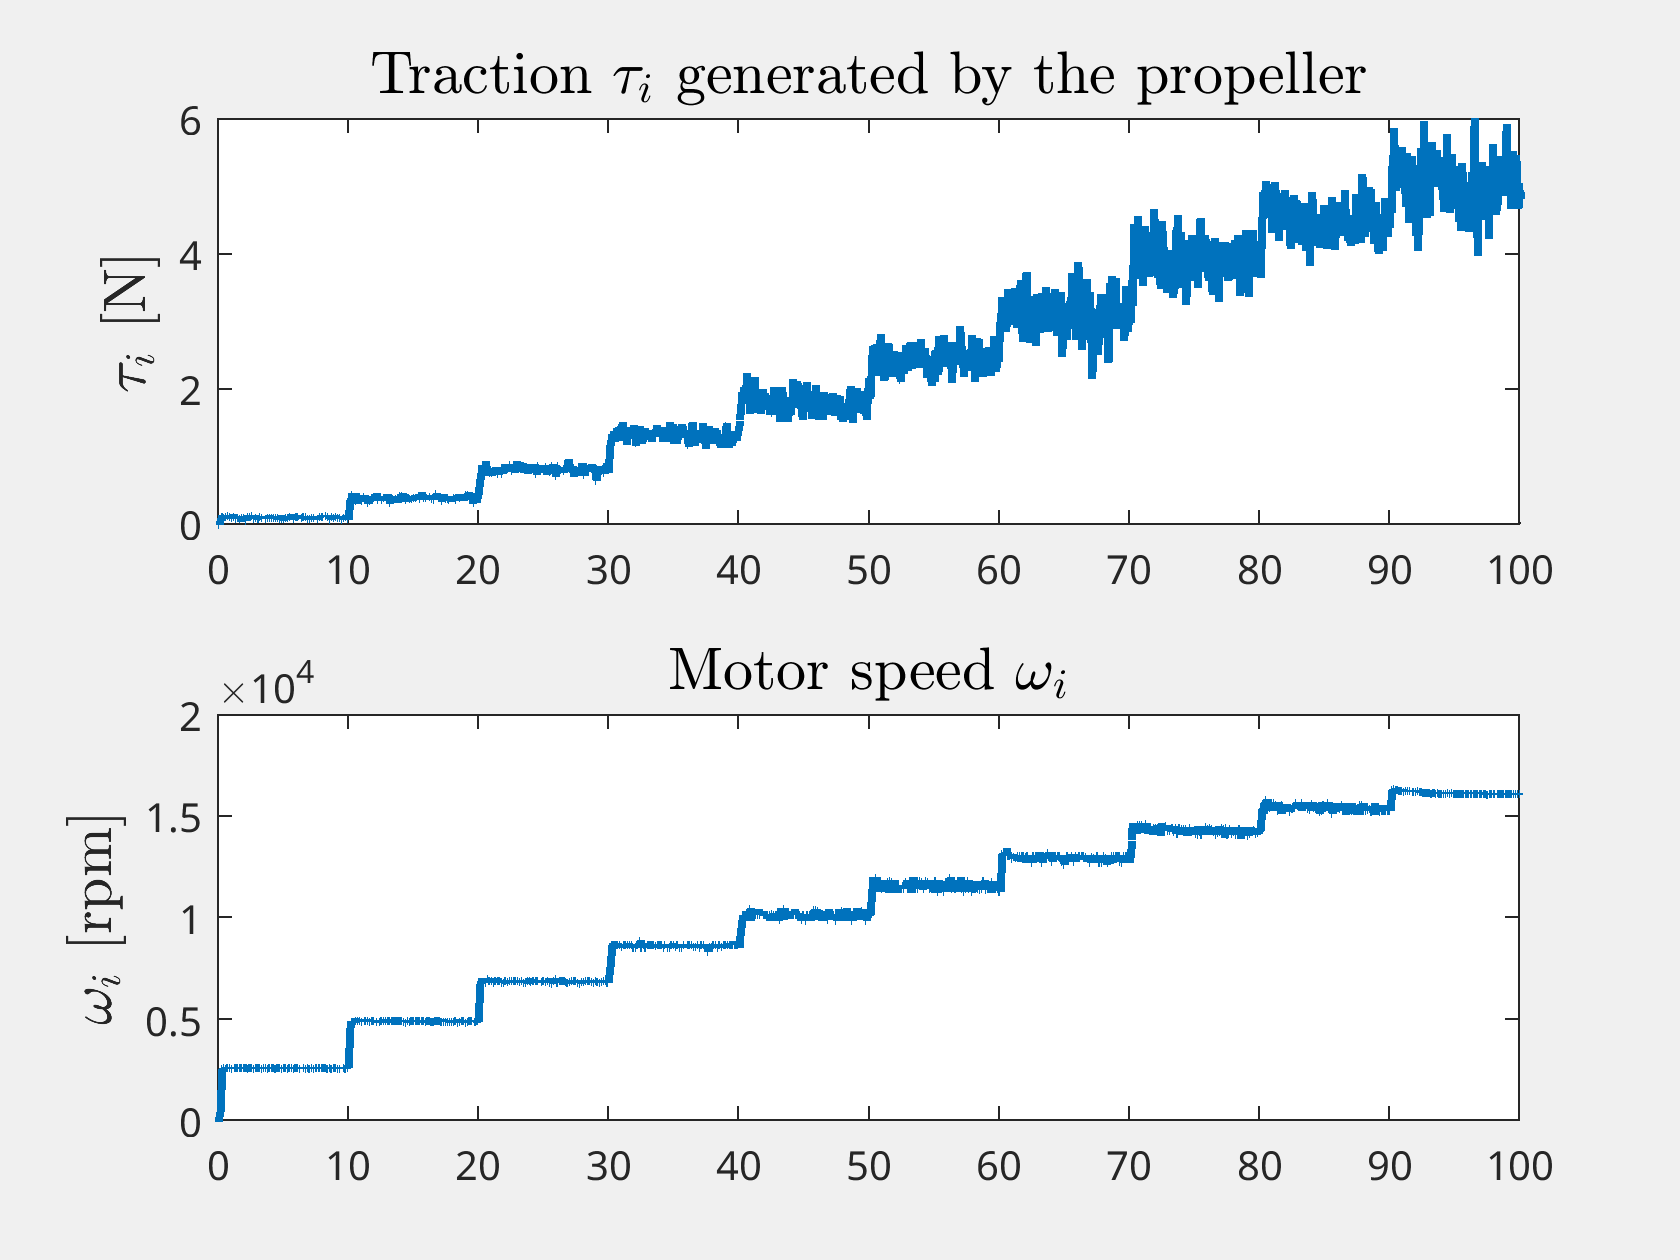
\includegraphics[trim=0cm 0cm 0cm 0cm,clip,width=0.5\columnwidth]{figures/ident_motor March 27 2024 1651.png}}
        \caption{Réponse entrée-sortie de l'ensemble moteur/hélice.}
        \label{fig:IOmot}
    \end{figure}
    
    Pour effectuer, l'identification des 3 coefficients principaux (diagonaux) de la matrice d'inertie, nous avons réalisé un montage d'un système de pendule bifilaire. Cette méthode est largement utilisée dans le domaine des drones \cite{Jardin2007OptimizedMO}, et est basée sur la période d'oscillation autour de chacun des trois axes ($x_{{\text{b}}}$, $y_{\text{b}}$, $z_{\text{b}}$) du drone, lequel est suspendu par deux fils, ce qui forme un pendule de torsion comme le montre la Fig. \ref{fig:BifilarPend}.

    \begin{figure}[ht!]
        \centerline{
        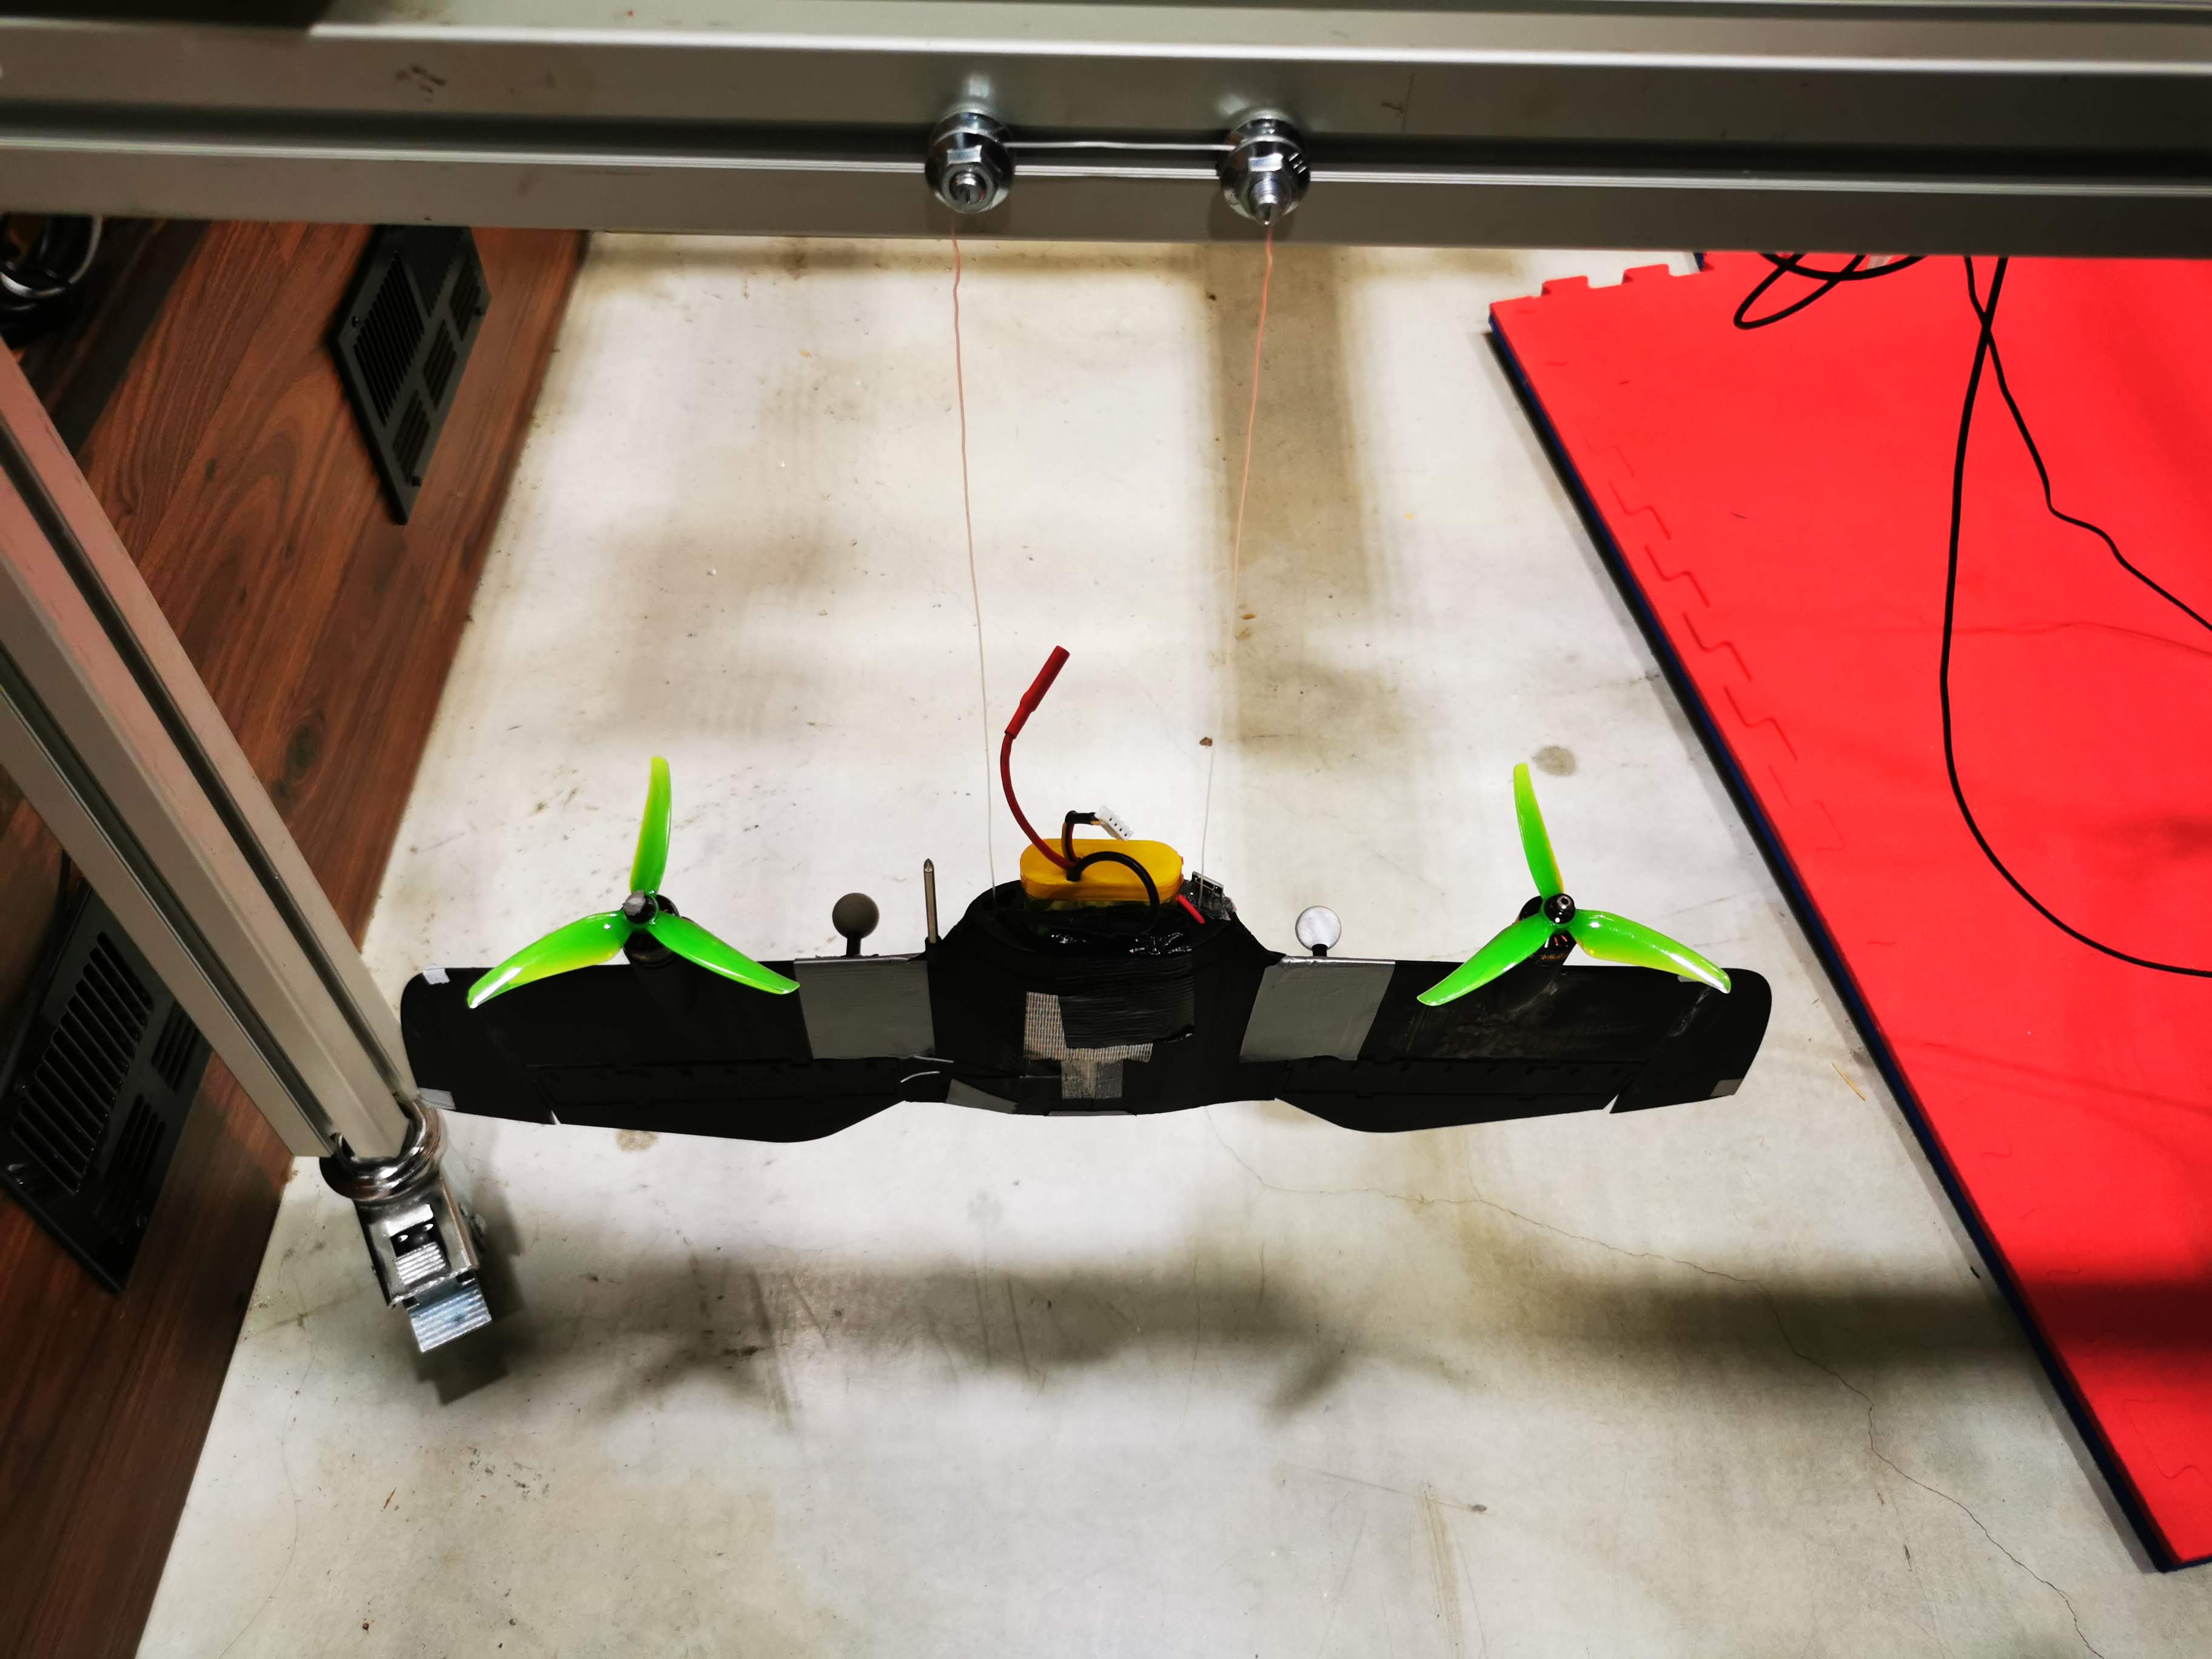
\includegraphics[trim=20cm 15cm 23cm 0cm,clip,width=0.4\columnwidth]{figures/IMG_20230609_085023.jpg}}
        \caption{Montage d'un pendule bifilaire pour l'identification de l'inertie ($\boldsymbol{J}$) de DarkO.}
        \label{fig:BifilarPend}
    \end{figure}

    Lors de la mesure, l'autopilote est utilisé pour réaliser une acquisition, à 500 Hz, de l'orientation du drone. Le drone est positionné avec un angle non nul vis-à-vis de la position d'équilibre du pendule bifilaire puis il est lâché sans vitesse initiale. Le couple de rappel engendré par les deux fils engendre des oscillations amorties (Voir la figure \ref{fig:BifilarPend_meas}). Il est nécessaire de connaitre la longueur des fils $h$ ainsi que leur écartement $D$ pour réaliser l'identification. Ces valeurs sont mesure directement sur le banc de mesure pour chacune des trois configurations.

    Une fois la mesure réalisée, nous utilisons l'outil \textit{Simulink Design Optimization} pour obtenir les valeurs de l'amortissement visqueux $C$, et de l'inertie sur l'axe mesuré $I$ à partir du modèle suivant :
    \begin{align*}
        \ddot{\theta} +  \frac{C}{I}\dot{\theta} + \left(\frac{mgD^2}{4Ih}\right)\frac{\sin\theta}{\sqrt{1 - 0.5\left(\frac{D}{h}\right)^2(1 - \cos\theta)}} = 0
    \end{align*}
    où $\theta$ est l'angle mesuré par l'autopilote à l'aide du code d'estimation d'état utilisant le gyroscope, l'accéléromètre et l'Optitrack.
    

    \begin{figure}[ht!]
    \centerline{
    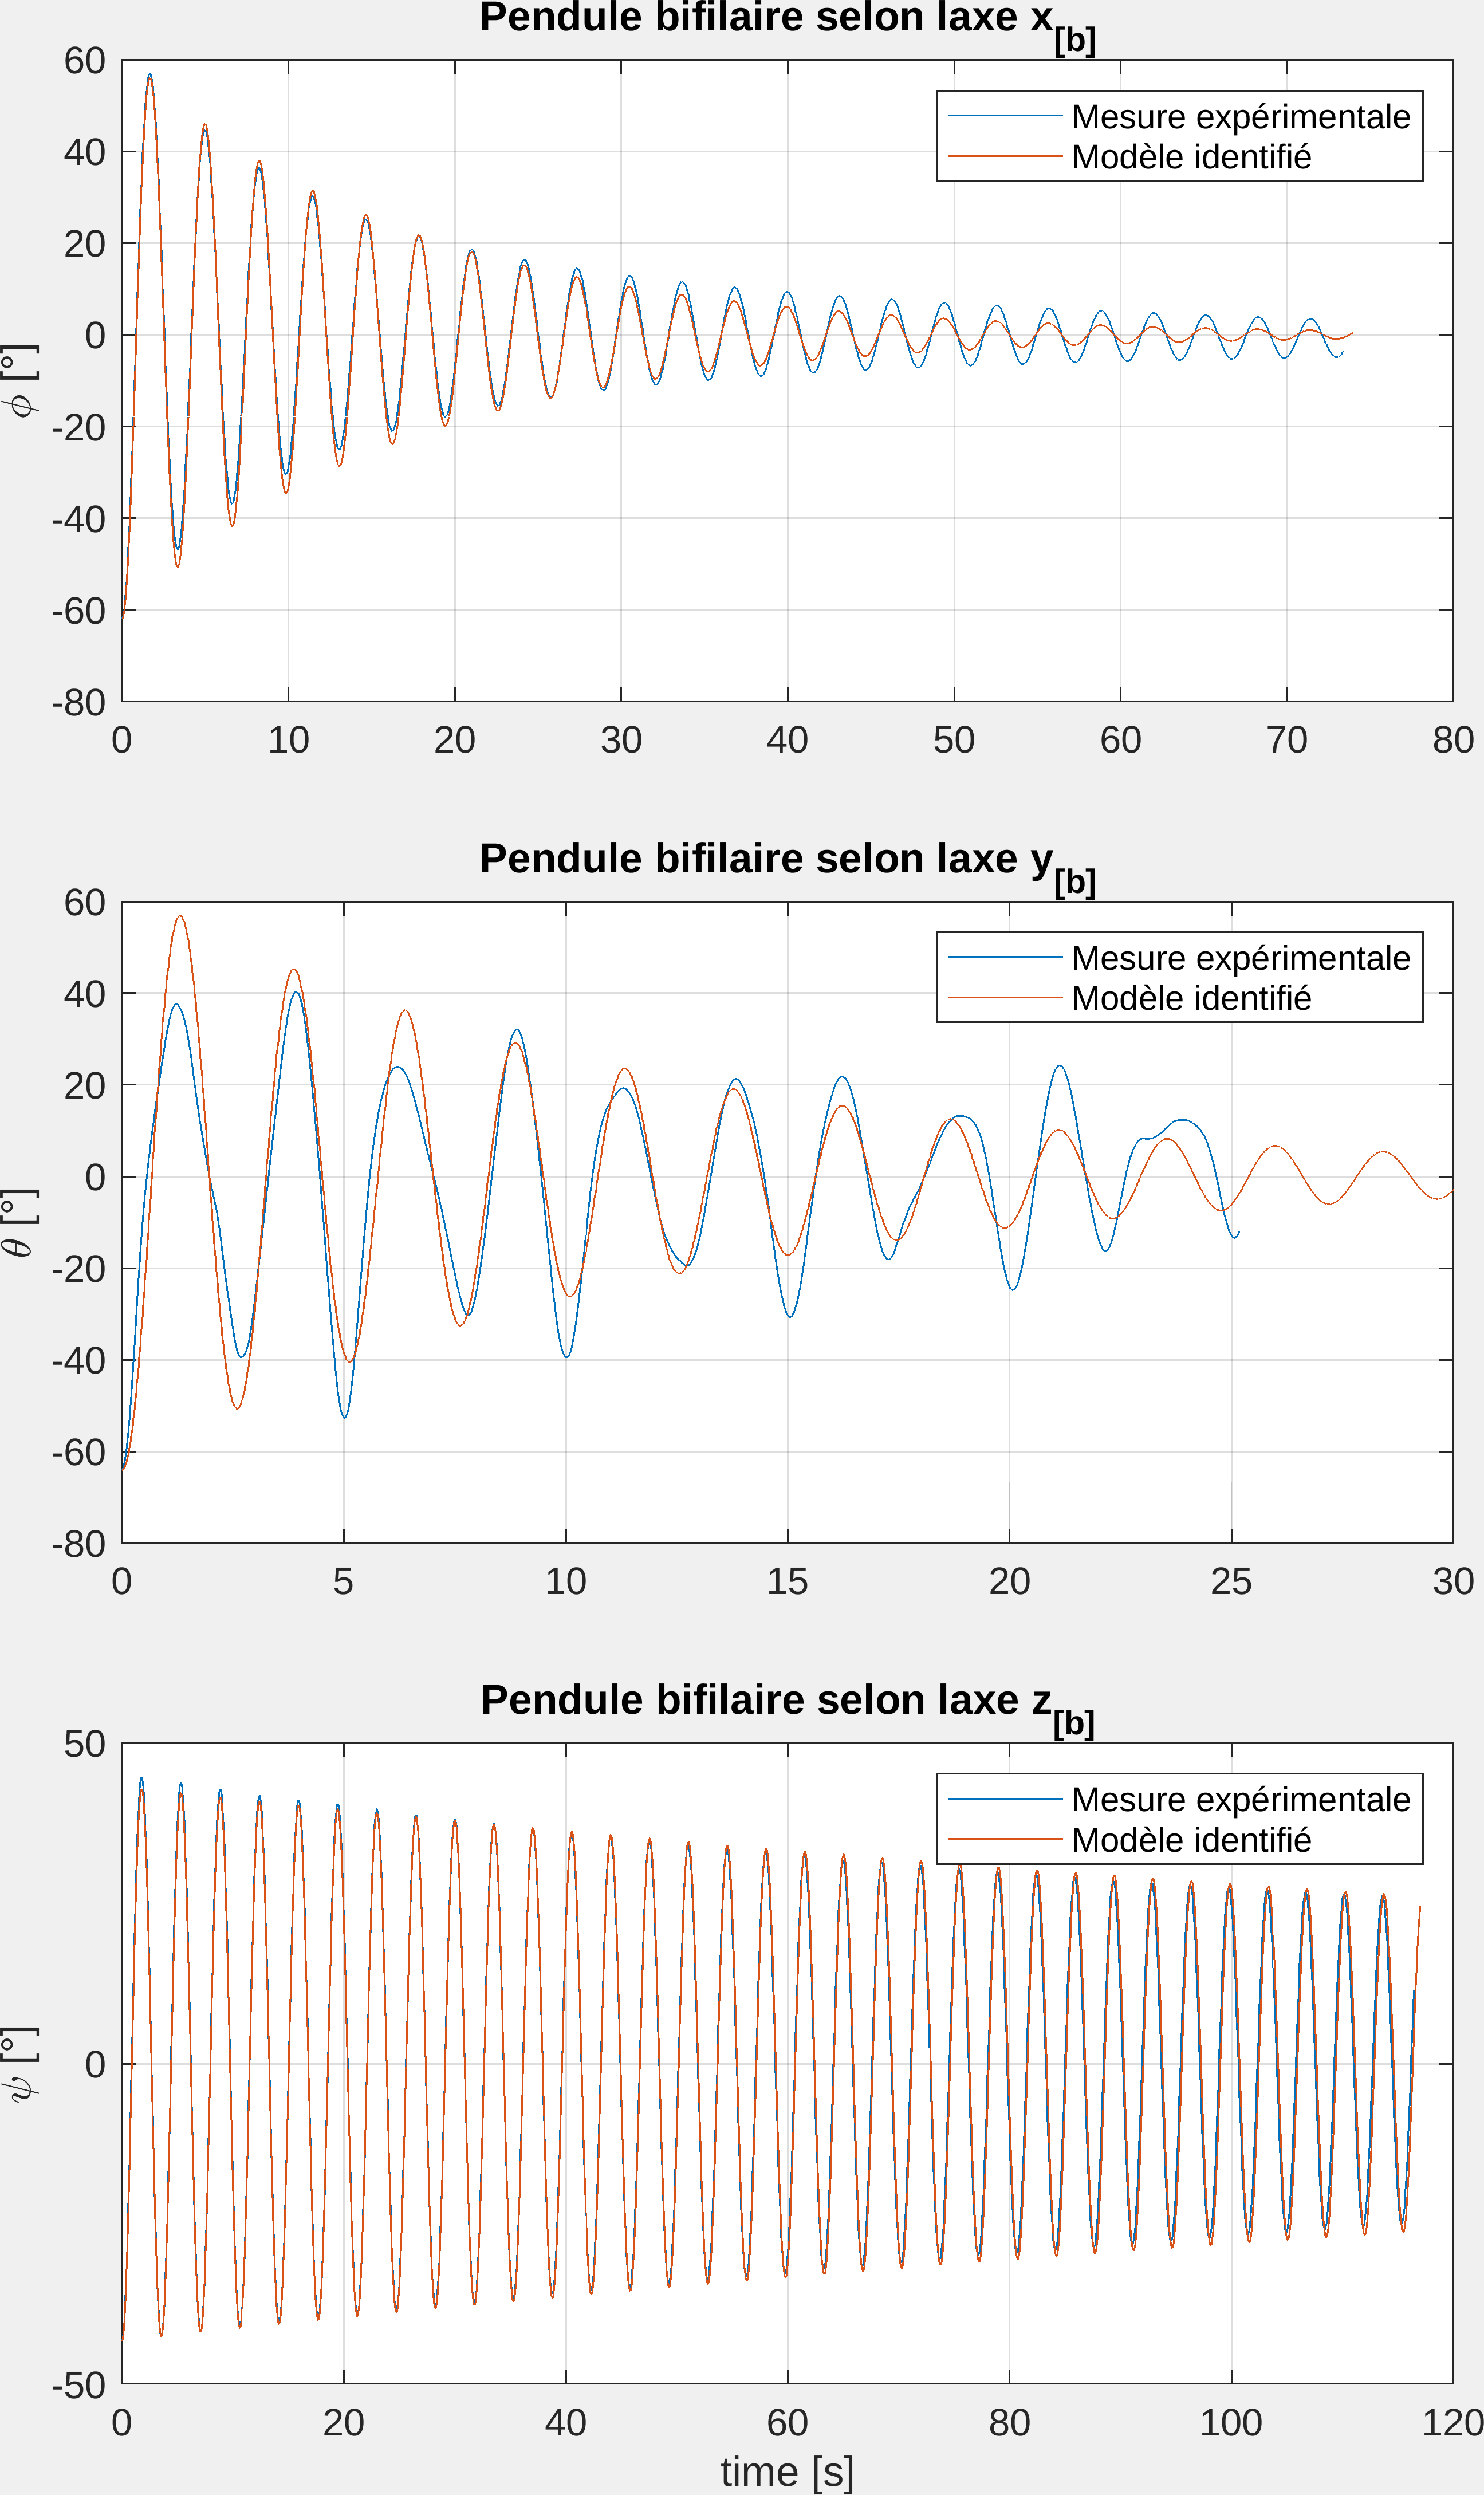
\includegraphics[trim=0cm 0cm 0cm 0cm,clip,width=0.6\columnwidth]{figures/ident_inertia.png}}
    \caption{Identification de l'inertie ($\boldsymbol{J}$), à partir des mesures issues du pendule bifilaire \ref{fig:BifilarPend}.}
    \label{fig:BifilarPend_meas}
    \end{figure}
    \todo{ajouter explication sur l'indentification}


    
    Les autres coefficients ont été estimés à l'aide d'un montage sur un capteur de force et moment à 6 DOF.
    \begin{figure}[ht!]
        \centering
        \resizebox{.9\textwidth}{!}{%
        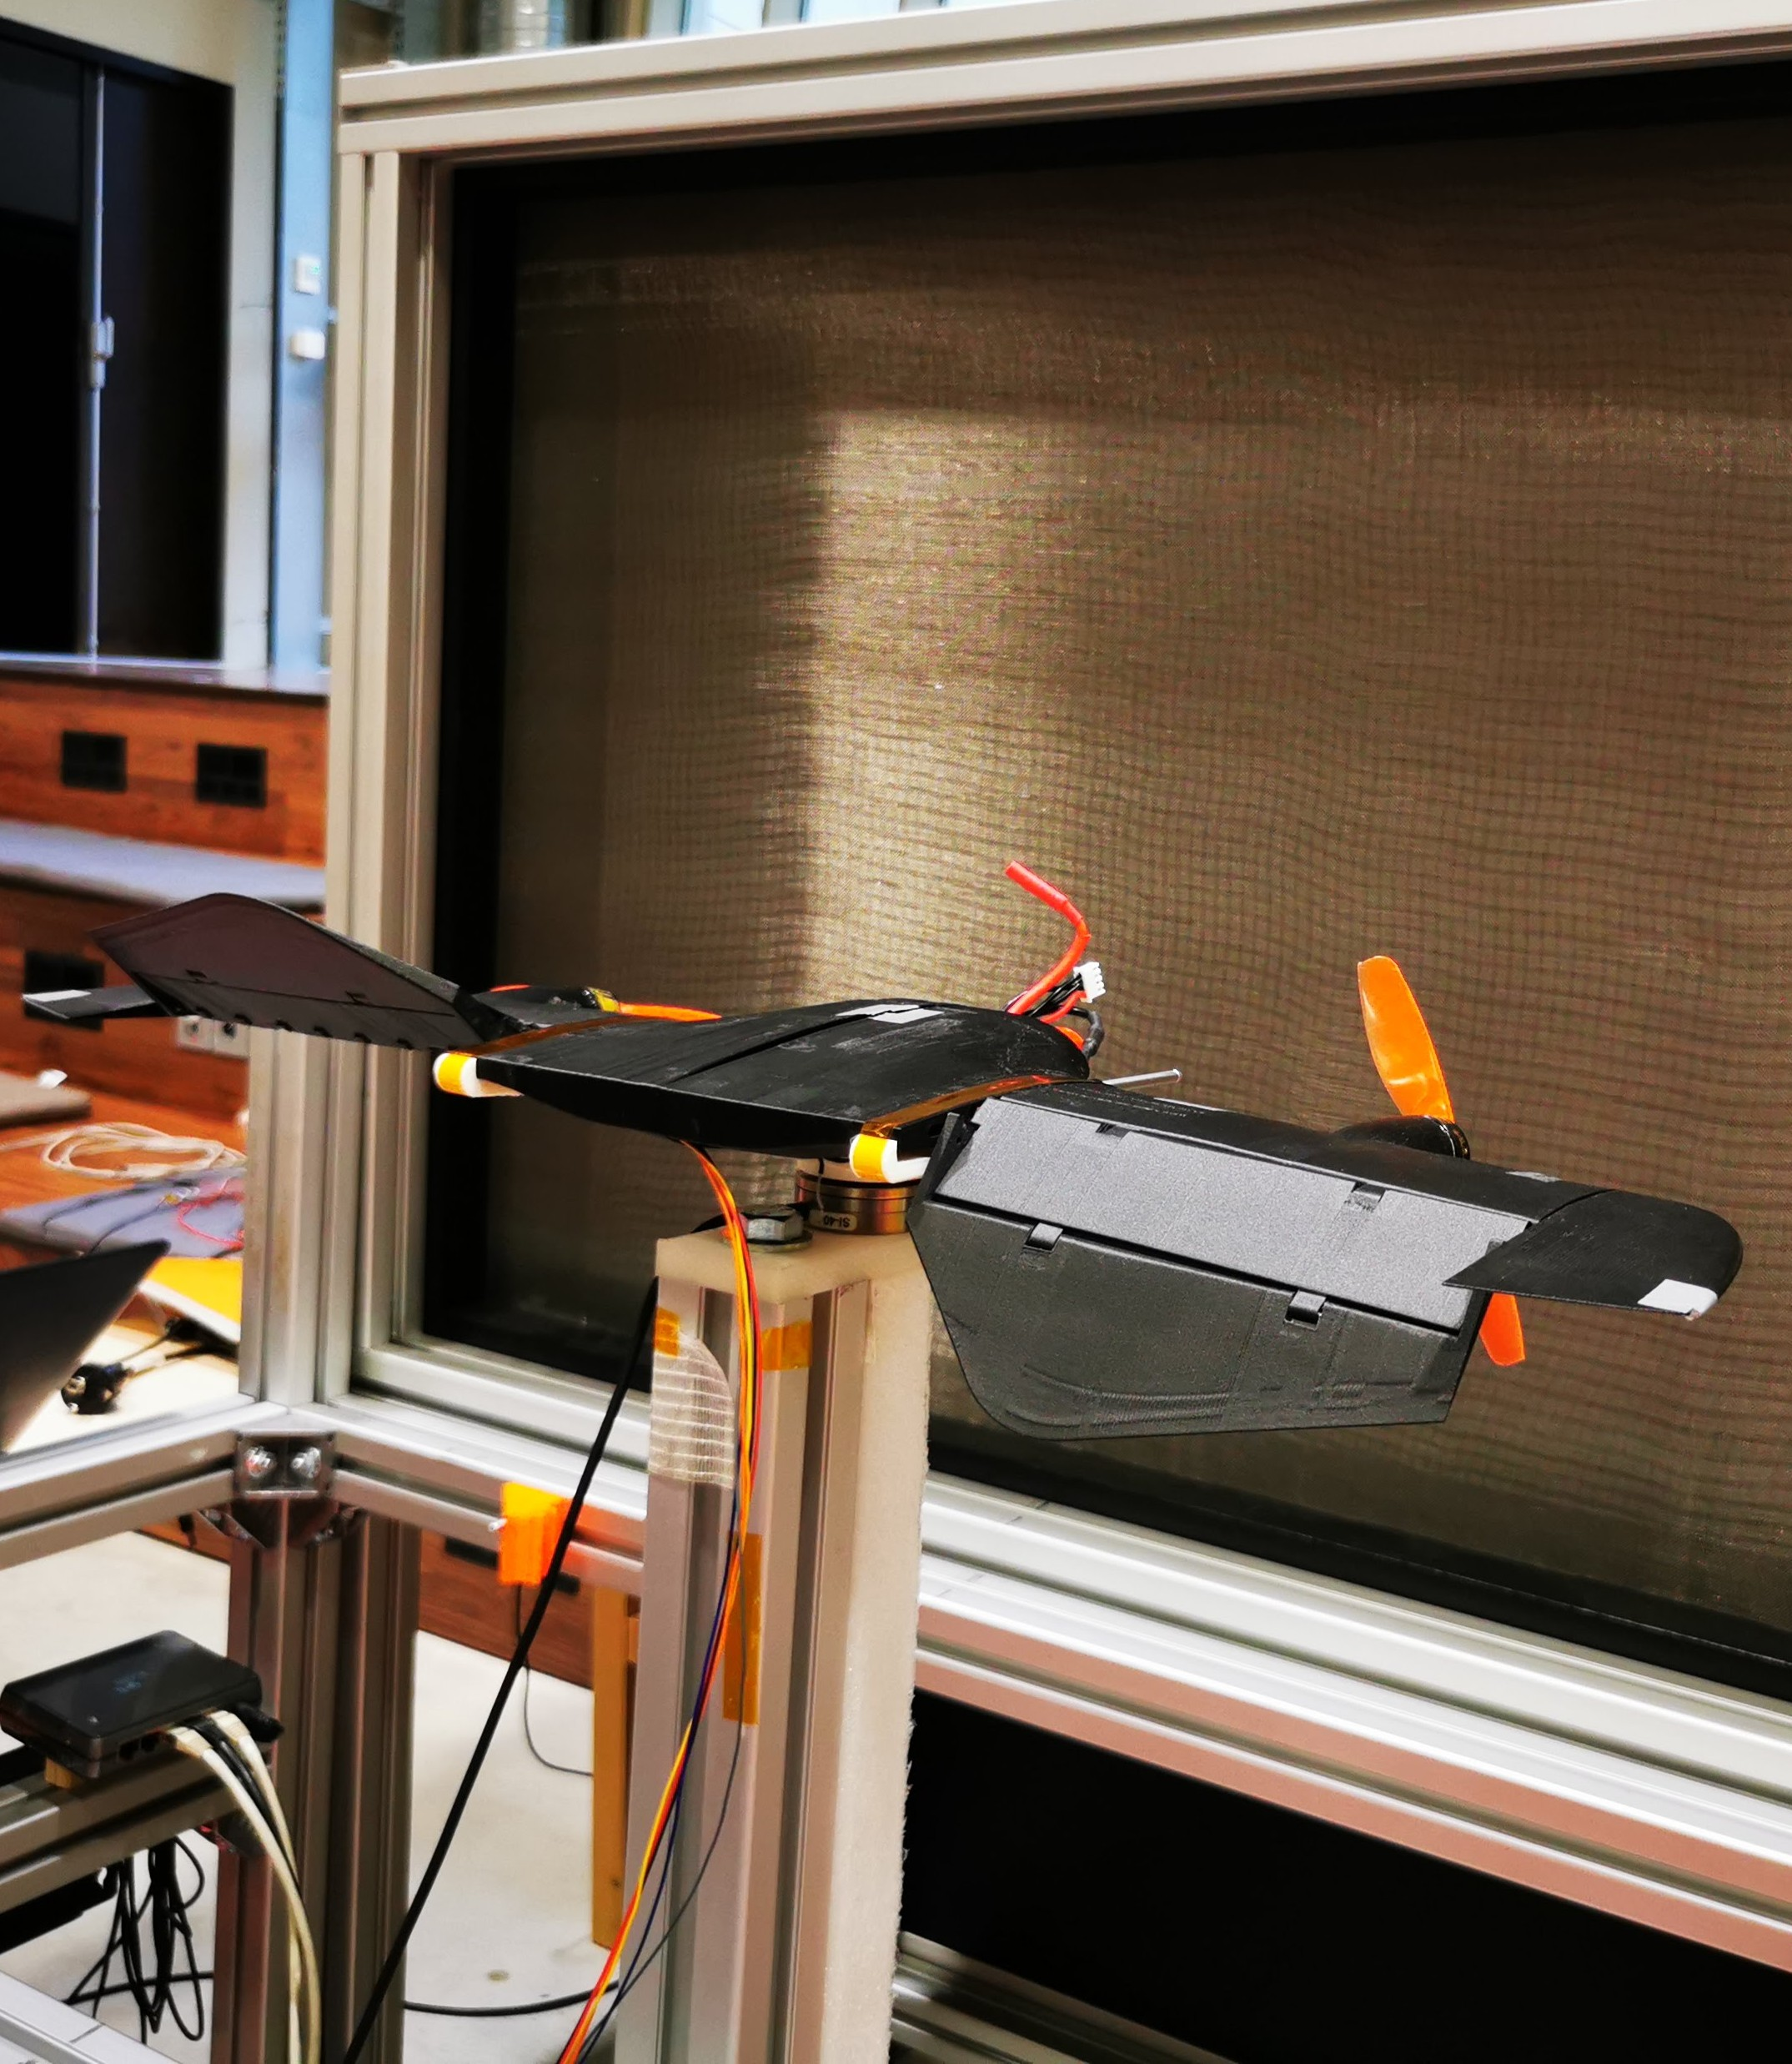
\includegraphics[height=3cm]{figures/montage_ident_arr.jpg}
        \quad
        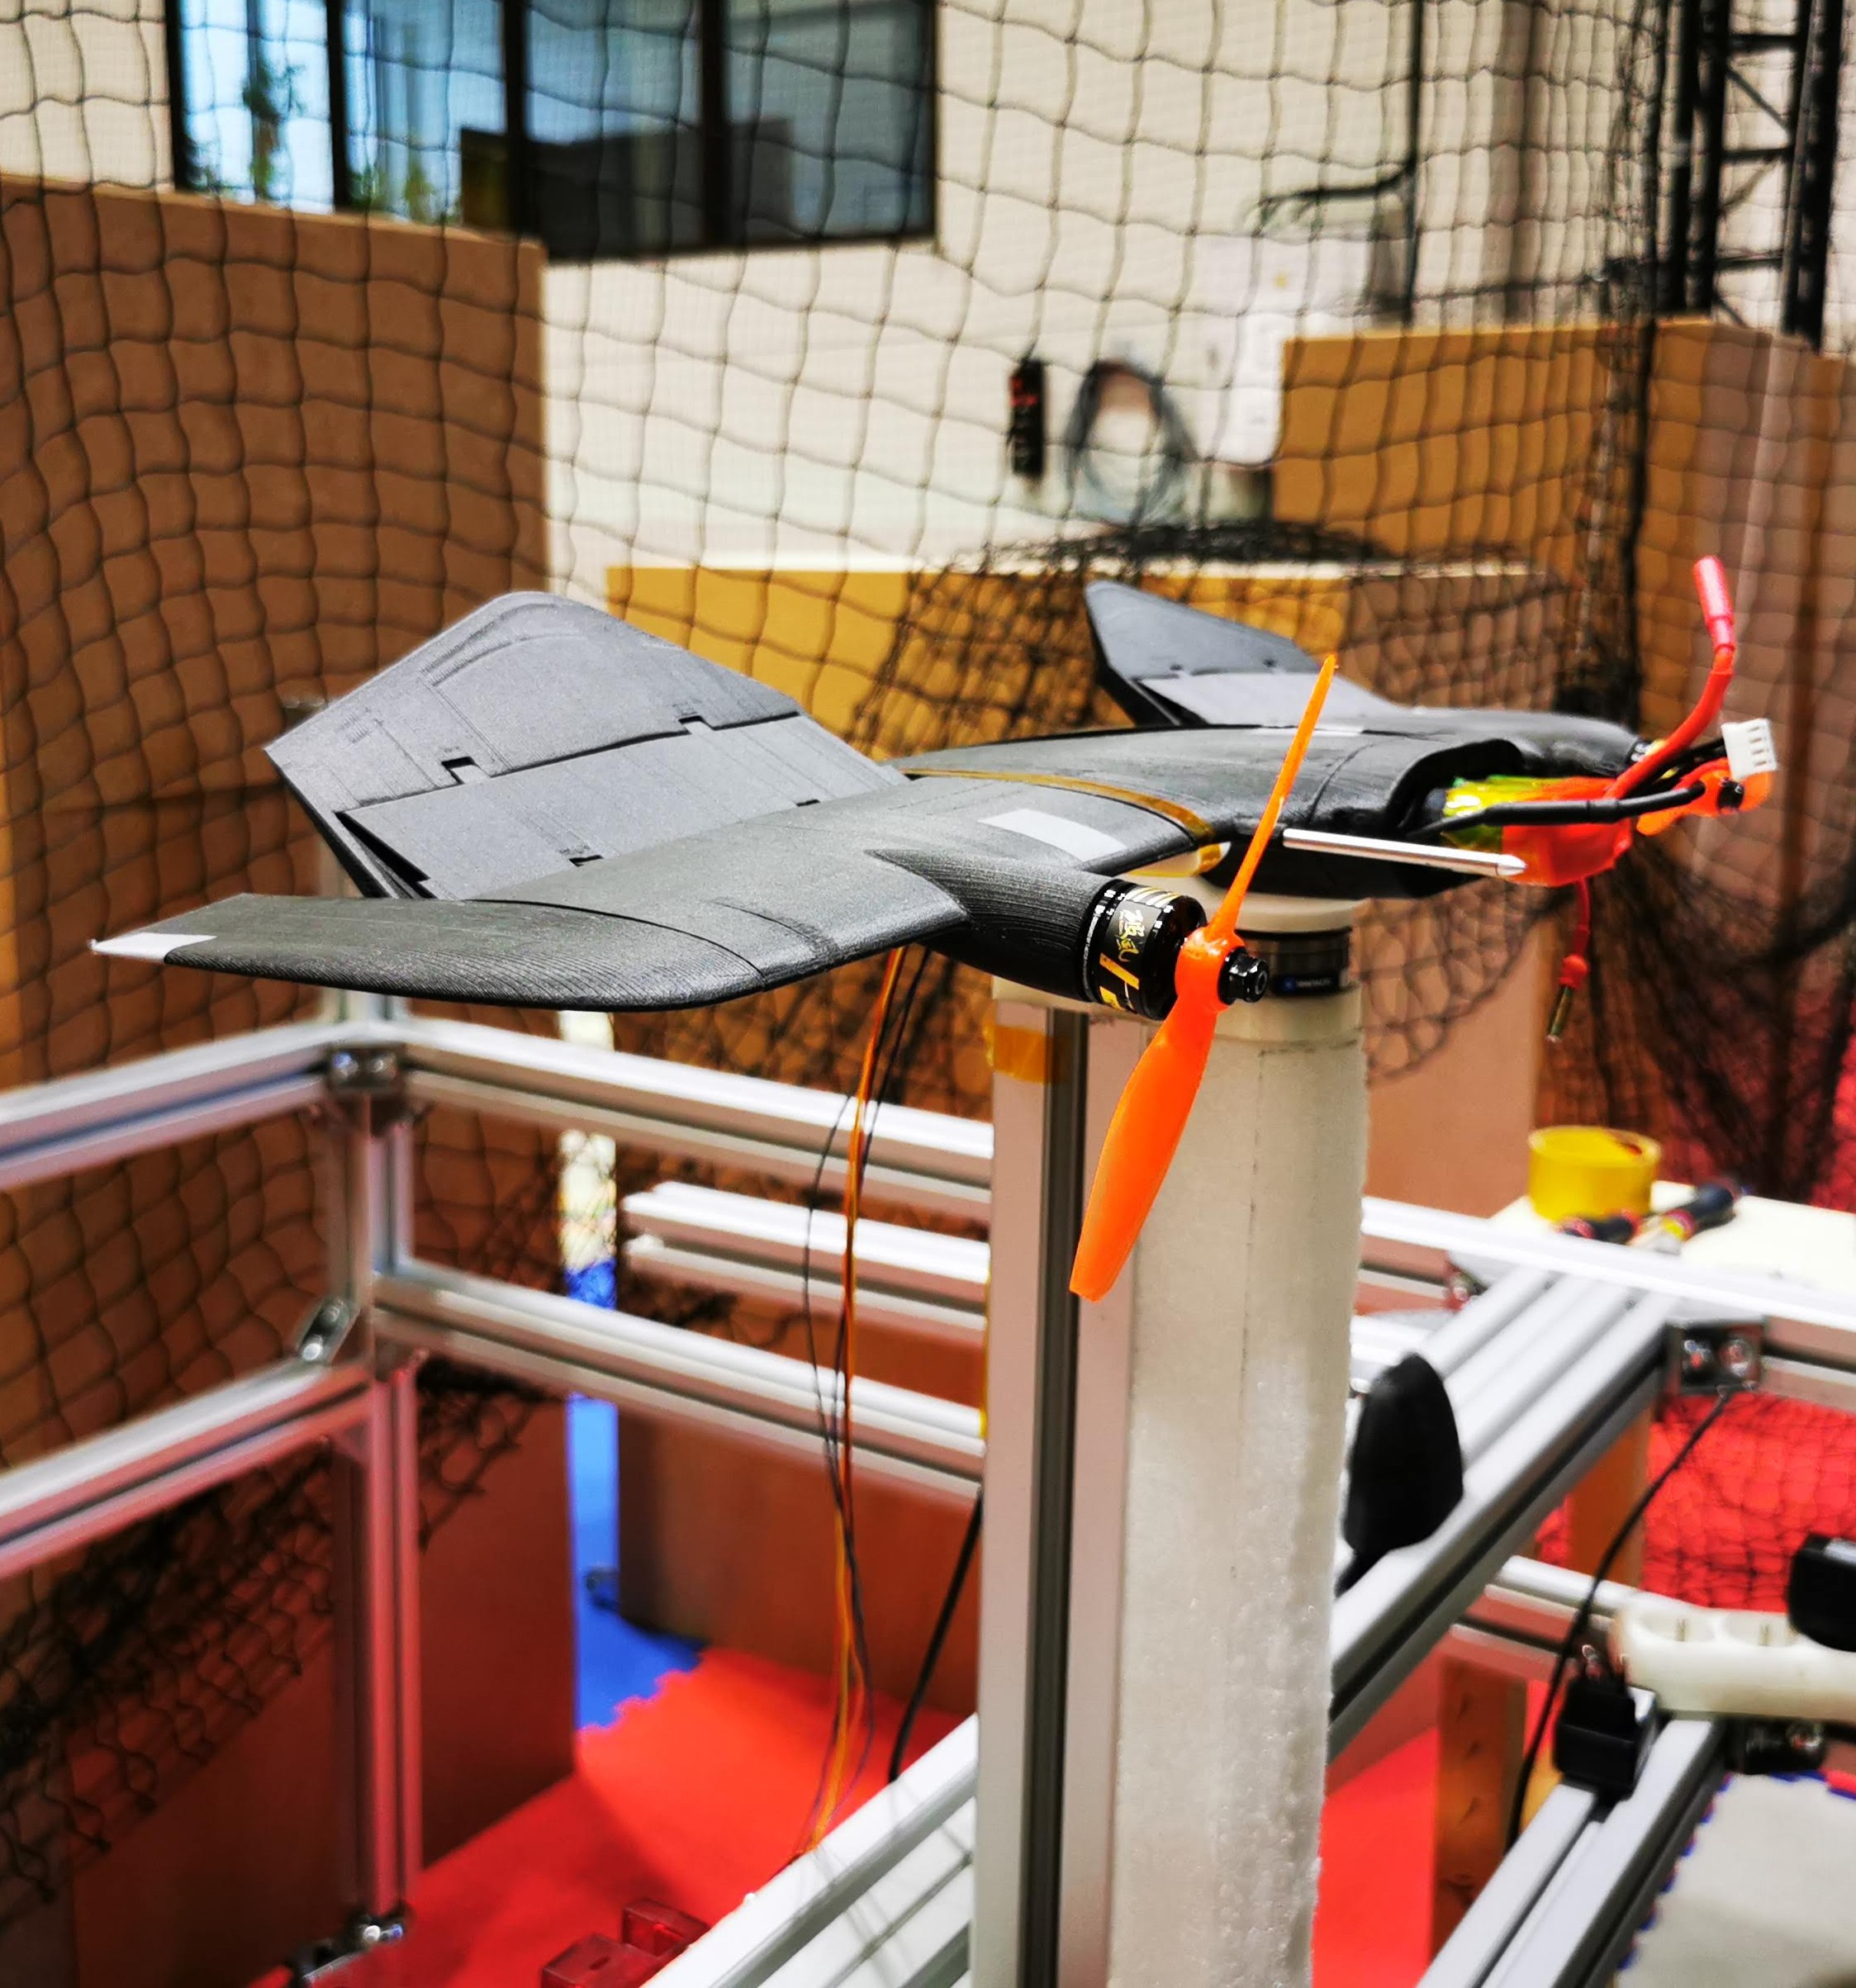
\includegraphics[height=3cm]{figures/montage_ident_face.jpg}
        }
        \caption{Montage de DarkO sur un banc de mesure face à une soufflerie ouverte.}
        \label{fig:montage_ident}
    \end{figure}
    Ces mesures permettent d'estimer la surface. Il est intéressant de noter que la surface soufflée par les hélices représente 67 \% de la surface totale du drone.
    

\subsection{Modélisation des actionneurs}
    \label{sec:saturation}
    Les actionneurs de DarkO ont des dynamiques qui limitent leur action en terme d'amplitude et de vitesse.

    Pour les moteurs électriques générant la traction par les hélices, il existe deux causes de saturation. Une saturation à haute vitesse liée à  la tension maximale du moteur et une saturation basse vitesse liée à la vitesse minimale de commutation de bobine du moteur, pour maintenir la rotation. De plus, ces saturations permettent d'obtenir un modèle réaliste à énergie finie. Elles correspondent à la contrainte suivante : $\omega_i \in [2500,~16000]~rpm = [262,~1675]~\SI{}{\radian\per\second}$, $i=1,2$. En termes de dynamique, nous avons représenté la chaîne d'actionnement du moteur (composée de l'ESC, du moteur et de l'hélice) par une fonction de transfert du premier ordre ayant une constante de temps égale à \SI{0,0125}{\second}, ce qui fournit un système d'actionnement assez agressif.

    Les saturations impactant les élevons proviennent des limites physiques des servomoteurs et du débattement limité par la forme de l'UAV, $\delta_i \in [-30~; 30]\text{\textdegree}$, $i=1,2$. La saturation la plus importante ici est peut-être la bande passante de l'actionneur (due à l'actionnement du servomoteur), qui est modélisée par une fonction de transfert du premier ordre avec une constante de temps \SI{0,05}{\second}. 

\section{Équilibres stationnaires}
    \subsection{Équilibre stationnaire sans vent}
        \label{sec:eq_nowind}

        Nous proposons une modification du vecteur de commande, dans le cas d'un équilibre sans vent $\boldsymbol{w}_{\mathrm{eq}} = 0$, basé sur le couplage des actionneurs. 
        \begin{align}
            \label{eq:vector_u_nowind}
            \boldsymbol{u}_{\text{nowind}} := \begin{bmatrix}\tau_{1}  \!&\! \tau_{2}  \!&\! \delta_{1}\tau_{1} \!&\! \delta_{2}\tau_{2} \end{bmatrix}^\top
        \end{align}
        Nous soulignons que le vecteur $\boldsymbol{u}_{\text{nowind}}$ dans \eqref{eq:vector_u_nowind} correspond à une transformation non inversible des actionneurs de DarkO correspondant à $\boldsymbol{u} := \begin{bmatrix}\tau_{1}  \!&\! \tau_{2}  \!&\! \delta_{1} \!&\! \delta_{2} \end{bmatrix}^\top$ (\eqref{eq:vector_u}). Néanmoins, si l'on impose les contraintes de saturation décrites dans la section~\ref{sec:saturation}, il est possible de déterminer de manière unique $\boldsymbol{u}$ à partir d'une valeur souhaitée de $\boldsymbol{u}_{\text{nowind}}$ dans \eqref{eq:vector_u_nowind}, car les valeurs positives non nulles de $\tau_{1}$ et $\tau_{2}$ peuvent être déterminées à partir des deux premières composantes de $\boldsymbol{u}_{\text{nowind}}$, puis $\delta_1$ et $\delta_2$ sont facilement construites à partir des deux dernières composantes de $\boldsymbol{u}_{\text{nowind}}$. 

        Nous obtenons un modèle linéaire vis-à-vis de sa commande, dérivé de \eqref{eq:dyna_simp} en imposant  $\boldsymbol{w} = 0$,
        \begin{subequations}\label{eq:withouwind}
        \begin{align}
                \boldsymbol{\dot p} &=  \boldsymbol{v}, \quad &
                m\boldsymbol{\dot v} &= - m\boldsymbol{g} +  \boldsymbol{R}(\boldsymbol{q})\boldsymbol{F}\boldsymbol{u}_{\text{nowind}},\\
                \boldsymbol{\dot q} &= \frac{1}{2}\boldsymbol{q} \otimes \smallmat{0 \\ \boldsymbol{\omega}_{\text{b}}} \quad & \boldsymbol{J} \boldsymbol{\dot \omega}_{\text{b}} &= \! \shortminus \skewsym{\boldsymbol{\omega}_{\text{b}}}\!J\boldsymbol{\omega}_{\text{b}} \! + \! \boldsymbol{M}\boldsymbol{u}_{\text{nowind}},
        \end{align}
        \end{subequations}
        avec les matrices
        \begin{align}
            \label{eq:FandM}
            \left[ \begin{array}{c|c}\!\boldsymbol{F}\!&\!\boldsymbol{M}\!\end{array} \right] := \left[ \begin{array}{cccc | cccc} a_{\text{f}} & a_{\text{f}} & 0 & 0 & a_{\text{m}} & -a_{\text{m}} & b_{\text{m}} & -b_{\text{m}} \\  0 & 0 & 0 & 0 & 0 & 0 & c_{\text{m}} & c_{\text{m}} \\ 0 & 0 & b_{\text{f}} & b_{\text{f}} & d_{\text{m}} & -d_{\text{m}} & 0 & 0 \end{array} \right]
        \end{align}
        et les scalaires
            \begin{align*}
                \left[\!\! \begin{array}{c|c} 
                a_{\text{f}} & b_{\text{f}} \\ \hline
                a_{\text{m}} & b_{\text{m}} \\ \hline
                c_{\text{m}} & d_{\text{m}}
                \end{array} \!\!\right] \!=\!
                \left[\begin{array}{c|c}
                1-\frac{S_{\text{wet}}}{4S_{\text{p}}} C_{\text{d}}  & -\frac{S_{\text{wet}}}{4S_{\text{p}}}C_{\ell}\xi_{\text{f}} \\ \hline
                \frac{k_{\text{m}} }{k_{\text{f}}}  &   \! \frac{S_{\text{wet}}}{4S_{\text{p}}}a_{y}C_{\ell}\xi_{\text{f}} \!\\ \hline
                \!\! \frac{S_{\text{wet}}}{4S_{\text{p}}} \Delta_{\text{r}}C_{\ell}\xi_{\text{m}} \!\! & 
                p_{y}+\frac{S_{\text{wet}}}{4S_{\text{p}}} a_{y} C_{\text{d}}
                \end{array}\right].
            \end{align*}


        Tous les couples d'équilibre $(\boldsymbol{u}_{\text{nowind}}, \boldsymbol{x}) = (\boldsymbol{u}_{\text{nowind},\text{eq}}, \boldsymbol{x_{\text{eq}}})$ sont paramétré par une rotation arbitraire autour de l'axe $z_{[\text{i}]}$ définit par $\beta \in \left[-\sqrt{\frac{1}{2}},\sqrt{\frac{1}{2}}\right]$. Le point d'équilibre a pour expression
        \begin{subequations}
            \label{eq:equilibria}
            \begin{align}
                \label{eq:bar_u}
                \boldsymbol{u}_{\text{nowind},\text{eq}} = \frac{mg}{( 1-\frac{S_{\text{wet}}}{4S_{\text{p}}} C_{\text{d}})} [1~1~0~0]^\top\\
                \boldsymbol{q}_{\text{eq}} = [\eta_{\text{eq}} ~\boldsymbol{\epsilon}_{\text{eq}}^\top]^\top = \smallmat{\sqrt{\frac{1}{2}-\beta} & \beta & \frac{2\beta^{2}-1}{2\sqrt{\frac{1}{2}-\beta}} & \beta}^\top.
            \end{align}
        \end{subequations}
        En présence d'un vent nul, le degré de liberté $\beta$ permet d'orienter le drone dans n'importe quelle direction horizontale.

    \subsection{Équilibre stationnaire en présence de vent}
    À partir des modèles \eqref{eq:dyna_orig} et \eqref{eq:dyna_simp}, nous caractérisons un équilibre stationnaire en présence d'un vent constant $\boldsymbol{w}_{\mathrm{eq}} =\smallmat{w_x \\ w_y \\w_z} \in \real^3$ exprimé dans le repère inertiel, tel que $\smallmat{w_x \\ w_y} \neq 0$, c'est-à-dire qu'il existe toujours un vent horizontal non nul.
    Ainsi, pour chaque position de référence $\boldsymbol{p}_{\text{eq}} \in \real^3$, 
    un ensemble de couple état/commande possible est $(\boldsymbol{u}_{\text{eq}}, \boldsymbol{x}_{\text{eq}}) = (\boldsymbol{u}_{\text{eq}}, \boldsymbol{p}_{\text{eq}}, \boldsymbol{v}_{\text{eq}}, \boldsymbol{q}_{\text{eq}}, \boldsymbol{\omega}_{\text{b},\text{eq}})$
    obtenu à l'aide de
    \begin{subequations}
    \label{eq:equilibrium}
    \begin{align}
    \label{eq:ueq}
            &\boldsymbol{u}_{\text{eq}} = \begin{bmatrix} \tau & \tau & \delta & \delta \end{bmatrix}^\top\\
            & \boldsymbol{q}_{\text{eq}} = \boldsymbol{q}_{\mathrm{eq}\psi} \otimes  \boldsymbol{q}_{\mathrm{eq}\theta} \label{eq:qeq}\\
            &\boldsymbol{\omega}_{\text{b},\text{eq}} = 0 , \quad \boldsymbol{v}_{\text{eq}} = 0, 
    \end{align}
    \end{subequations}
    où nous définissons deux quaternions $\boldsymbol{q}_{\mathrm{eq}\psi}$ et $\boldsymbol{q}_{\mathrm{eq}\psi}$ permettant d'exprimer l'ensemble des conditions de vent dans le repère inertiel vers un repère tourné où le vent est toujours contenu dans le plan $x-z$. Grâce à cette transformation, nous exprimons un ensemble continue d'équilibre en présence de vent. 

    \begin{align}
    \label{eq:qtheta}
        \boldsymbol{q}_{\mathrm{eq}\theta} &:= \begin{bmatrix} \cos(\frac{\theta}{2}) & 0 & \sin(\frac{\theta}{2}) & 0 \end{bmatrix}^\top
    \end{align}
    \begin{align}
    \label{eq:qpsi}
        \boldsymbol{q}_{\mathrm{eq}\psi} &:= \begin{bmatrix} \cos(\frac{\psi}{2}) & 0 & 0 & \sin(\frac{\psi}{2}) \end{bmatrix}^\top.
    \end{align}
    Les paramètres de l'équilibre sont la rotation horizontale $\psi = \arctan(w_{x}, w_{y})$, l'angle d'inclinaison $\theta$, la poussée des hélices $\tau$, et la déflexion des élevons $\delta$. Ils peuvent être obtenus à partir de l'algorithme~\ref{alg:eq}. 

    \begin{algorithm}
    \caption{Obtention des paramètres d'équilibre en \eqref{eq:equilibrium}.}
    \label{alg:eq}
    \hspace*{.1cm} \textbf{Entrée} : Vecteur vent $\boldsymbol{w}_{\text{eq}} =\smallmat{w_x & w_y & w_z}^\top$ \\
    \hspace*{.1cm} \textbf{Sortie} : Paramètres $\psi$, $\theta$, $\tau$, $\delta$ dans \eqref{eq:equilibrium}
    \begin{algorithmic}[1]
        %\Require {\bf Input} values: $\boldsymbol{w} =\smallmat{w_x & w_y & w_z}^\top$ 
        %\Ensure  $\psi$, $\theta$, $\tau$, $\delta$
        \State Détermine l'angle $\psi = \text{atan2}(w_x, w_y)$ de manière à obtenir $\boldsymbol{q}_{\mathrm{eq}\psi}$ dans \eqref{eq:qpsi}  
        \State Détermine la perturbation tournée $\boldsymbol{w}_{\text{r}}$ avec la composante $y$ nulle, en utilisant $\boldsymbol{R}_{\psi}:= \smallmat{ \cos \psi & \sin \psi & 0 \\ -\sin \psi & \cos \psi & 0 \\ 0 & 0 & 1 }$, selon
        \begin{align}
        \label{eq:wh}
        \boldsymbol{w}_{\mathrm{r,eq}} := \smallmat{w_{\text{r}x} \\ 0 \\w_{\text{r}z}} :=  \boldsymbol{R}^\top(\boldsymbol{q}_{\mathrm{eq}\psi}) \boldsymbol{w}_{\mathrm{eq}} = \boldsymbol{R}^\top_{\psi} \boldsymbol{w}_{\mathrm{eq}}
        \end{align}

        \State Détermine l'angle d'inclinaison $\theta$ de manière à obtenir $\boldsymbol{q}_{\text{eq}\theta}$ dans \eqref{eq:qeq}:  
        \begin{align}
        \label{eq:theta_alg}
            \theta = -\tan^{-1}\left(\frac{w_{\text{r}z}}{w_{\text{r}x}} + \frac{2mg}{\rho S \lVert \boldsymbol{w}_{\mathrm{eq}} \rVert C_{\ell}  (1-\frac{\xi_{\text{f}}}{\xi_{\text{m}}}) w_{\text{r}x} } \right)
        \end{align}
    \State Pour des raisons de commodité, nous définissons les scalaires 
        $$ 
        \left[\begin{array}{c|c} 
        \!\!a\!\!&\!\!b\!\! \\ \hline \!\!c\!\!&\!\! d\!\!\end{array}  \right] \!:=\! 
        \left[\begin{array}{c|c}
        2 S_{\text{wet}} C_{\ell} mg \sin{\theta} \xi_{\text{f}} &
        \! 2 S_{\text{wet}} C_{\text{d}} C_{\ell} \rho  \lVert \boldsymbol{w}_{\mathrm{eq}} \rVert  w_{x}^{\text{b}}\!\! \\ \hline
        \!\!-4 S S_{\text{p}} C_{\ell} \rho  \lVert \boldsymbol{w}_{\mathrm{eq}} \rVert  w_{x}^{\text{b}} \xi_{\text{f}}\!\! & \frac{b \xi_{\text{f}}}{2}
        \end{array}\right]
        $$ 
        et grâce à ces scalaires $(a,b,c,d)$, déterminons la traction des hélices $\tau$ dans \eqref{eq:ueq} comme
        \begin{align}
            \nonumber
            \tau &= \frac{S_{\text{p}}}{2 S_{\text{wet}} C_{\ell} \xi_{\text{f}} (4S_{\text{p}} -  S_{\text{wet}} C_{\text{d}} )} \Bigg( a+b+c+d + \Bigg[ (a+b+c \shortminus d)^2 \shortminus 4 (d^2+ac \shortminus bd)  \\ 
            & \quad
            \shortminus \frac{4 {w_{z}^{\text{b}}}^2 d}{ {w_{x}^{\text{b}}}^2 } (d+c) + \frac{4 w_{z}^{\text{b}}ad\cos{\theta}}{w_{x}^{\text{b}} C_{\ell} \sin{\theta} } \left(C_{\text{d}} - \frac{4 S_{\text{p}}}{S_{\text{wet}}}\right) \Bigg] ^{\frac{1}{2}} \Bigg),\label{eq:tau_alg}
        \end{align}
        où
        $$
        \bigmat{w_{x}^{\text{b}} \\ w_{z}^{\text{b}}} = \bigmat{   w_{\text{r}x} \cos{\theta} - w_{\text{r}z} \sin{\theta}\\
                    w_{\text{r}x} \sin{\theta} +  w_{\text{r}z} \cos{\theta} }.
        $$
        
        \State Déterminons la déflexion des élevons $\delta$ comme
        \begin{align}
        \label{eq:delta_alg}
            \delta = \frac{2mg\sin{\theta}}{\rho S \lVert \boldsymbol{w}_{\mathrm{eq}} \rVert C_{\text{d}}\xi_{\text{f}} w_{z}^{\text{b}}} + \frac{w_{x}^{\text{b}}}{\xi_{\text{f}}w_{z}^{\text{b}}} -  \frac{(4-\frac{S_{\text{wet}}}{S_{\text{p}}} C_{\text{d}})}{\rho S \lVert \boldsymbol{w}_{\mathrm{eq}} \rVert C_{\text{d}}\xi_{\text{f}} w_{z}^{\text{b}}} \tau.
        \end{align}

    \end{algorithmic}
    \hspace*{.1cm} \textbf{Retourne}:  $\psi$, $\theta$, $\tau$, $\delta$
    \end{algorithm}


    \begin{theorem}\label{thm:eqs}
    Pour tout vent constant, $\boldsymbol{w} =\smallmat{w_x & w_y & w_z}^\top \in \real^3$ ayant une composante horizontale non nulle $\smallmat{w_x \\ w_y}$,
    les équations \eqref{eq:qpsi}--\eqref{eq:qtheta} avec $\theta$, $\tau$ et $\delta$ sélectionné selon l'Algorithme~\ref{alg:eq} caractérisent un couple d'équilibre $(\boldsymbol{u}_{\text{eq}}, \boldsymbol{x}_{\text{eq}})$ pour la dynamique non linéaire \eqref{eq:dyna_orig} et \eqref{eq:dyna_simp}.
    
    \end{theorem}
    
    \begin{proof}
        Dans un premier temps, notons qu'avec l'expression de $\boldsymbol{R}$ \eqref{eq:matrix_rot} et l'expression de  $\psi$ dans l'étape 1 de l'Algorithme~\ref{alg:eq}, on peut définir la perturbation à l'équilibre tournée $\boldsymbol{w}_{\mathrm{r,eq}} := \boldsymbol{R}^\top_{\psi} \boldsymbol{w}_{\mathrm{eq}} :=    \boldsymbol{R}^\top(\boldsymbol{q}_{\mathrm{eq}\psi})\boldsymbol{w}_{\mathrm{eq}}$ (voir \eqref{eq:wh} dans l'Algorithme~\ref{alg:eq}),
        qui correspond à la rotation nécessaire pour aligner l'axe  $x_{[\text{b}]}$ du repère corps avec la direction du vent. Une fois que le drone est face au vent, il subit un vent avec une composante latérale $y$ nulle et il peut ajuster son angle d'inclinaison $\theta$ afin de générer la poussée et la portance nécessaires pour compenser les effets du vent dans les directions longitudinale et verticale (l'effet latéral est nul en raison de l'orientation spécifique de l'appareil $\psi$). Avec cette rotation $\psi$, il est possible d'exprimer le vent dans le repère corps comme étant
            \begin{align}
            \label{eq:wb}
                \boldsymbol{w}^{\text{b}}_{\mathrm{eq}} &:= 
                \begin{bmatrix}
                    w_{x}^{\text{b}} \\ 0 \\ w_{z}^{\text{b}}
                \end{bmatrix} \!=\! 
                \boldsymbol{R}^\top(\boldsymbol{q}_{\text{eq}\theta}) \boldsymbol{w}_{\mathrm{r,eq}}  \\
                &=\!\! \begin{bmatrix}
                    \cos{\theta} & 0 & -\sin{\theta}\\
                        0 & 1 & 0\\
                    \sin{\theta} & 0 & \cos{\theta}
                \end{bmatrix}^\top \!\! \begin{bmatrix}
                    w_{\text{r}x}\\
                    0\\
                    w_{\text{r}z}
                \end{bmatrix}
                \!\!=\!\!\begin{bmatrix}
                    w_{\text{r}x} \cos{\theta} - w_{\text{r}z} \sin{\theta}\\
                    0\\
                    w_{\text{r}x} \sin{\theta} +  w_{\text{r}z} \cos{\theta}
                \end{bmatrix}
            \nonumber
            \end{align}

        Nous insistons sur le fait que $w_{x}^{\text{b}}$ est toujours négatif et différent de zéro, car le drone est orienté dans la direction du vent grâce à la rotation engendré par $ \boldsymbol{q}_{\mathrm{eq}\psi}$, et suite à l'hypothèse $\smallmat{w_x \\ w_y} \neq 0$.
    
        L'équation \eqref{eq:dyna1} montre qu'il est nécessaire d'avoir $\boldsymbol{v}_{\text{eq}} = 0$ pour maintenir l'équilibre stationnaire. En multipliant \eqref{eq:dyna2} par $\boldsymbol{R}(\boldsymbol{q}_{\text{eq}})$ donné dans  \eqref{eq:wb}, nous l'exprimons dans le repère corps.
        Comme nous appliquons la même commande $\tau_{1} = \tau_{2} = \tau $ aux deux moteurs et la même commande au deux élevons $\delta_{1} = \delta_{2} = \delta$, nous obtenons pour les deux modèles \eqref{eq:dyna_orig} et \eqref{eq:dyna_simp}, l'équilibre des forces selon l'axe $x_{[\text{b}]}$ donné par
        \begin{align}
            & (2-\frac{S_{\text{wet}}}{2S_{\text{p}}} C_{\text{d}})\tau - \frac{1}{2}\rho S \lVert \boldsymbol{w}_{\mathrm{eq}} \rVert C_{\text{d}} \left(w_{x}^{\text{b}} - \xi_{\text{f}} \delta w_{z}^{\text{b}} \right) - mg \sin(\theta) = 0 \label{eq:forcex}
        \end{align}
        et l'équilibre des forces selon l'axe $z_{[\text{b}]}$ donné par
        \begin{align}\label{eq:forcez}
            - \frac{S_{\text{wet}}}{2S_{\text{p}}}\xi_{\text{f}} C_{\ell} \tau \delta - \frac{1}{2}\rho S \lVert \boldsymbol{w}_{\mathrm{eq}} \rVert C_{\ell} \left(w_{z}^{\text{b}} + \xi_{\text{f}} \delta w_{x}^{\text{b}} \right) + mg \cos(\theta) = 0
        \end{align}
        De manière similaire, à partir de \eqref{eq:dyna_orig_d} et \eqref{eq:dyna4}, l'équilibre des moments autour de l'axe $y_{[\text{b}]}$ permet d'obtenir
        \begin{align}\label{eq:momenty}
            \frac{S_{\text{wet}}}{2S_{\text{p}}}  \Delta_{\text{r}} \xi_{\text{m}} C_{\ell} \tau \delta + \frac{1}{2}\rho S \Delta_{\text{r}} \lVert \boldsymbol{w}_{\mathrm{eq}} \rVert C_{\ell} \left(w_{z}^{\text{b}} + \xi_{\text{m}} \delta w_{x}^{\text{b}} \right) = 0.
        \end{align}
        
        Pour calculer la solution du triplet ($\theta$,$\tau$,$\delta$) des trois équations d'équilibre \eqref{eq:forcex}--\eqref{eq:momenty}, ajoutons \eqref{eq:forcez} multiplié par $\Delta_{\text{r}} \xi_{\text{m}}$, à \eqref{eq:momenty} multiplié par $\xi_{\text{f}}$, de manière à annuler le premier terme et à obtenir
        \begin{multline*}
            \Delta_{\text{r}} \xi_{\text{m}} \left( - \frac{1}{2}\rho S \lVert \boldsymbol{w}_{\mathrm{eq}} \rVert C_{\ell} (w_{z}^{\text{b}} + \xi_{\text{f}} \delta w_{x}^{\text{b}}) + mg \cos(\theta) \right) \\+ \xi_{\text{f}} \left(\frac{1}{2}\rho S  \Delta_{\text{r}} \lVert \boldsymbol{w}_{\mathrm{eq}} \rVert C_{\ell} (w_{z}^{\text{b}} + \xi_{\text{m}} \delta w_{x}^{\text{b}})  \right) = 0,
        \end{multline*}
        qui est équivalent à
        \begin{align*}
            \frac{1}{2}\rho S  \Delta_{\text{r}} \lVert \boldsymbol{w}_{\mathrm{eq}} \rVert C_{\ell}  (\xi_{\text{f}} - \xi_{\text{m}}) w_{z}^{\text{b}} +   \Delta_{\text{r}} \xi_{\text{m}} mg \cos(\theta)  = 0,
        \end{align*}
        où ($w_{x}^{\text{b}}$,$w_{z}^{\text{b}}$) sont les première et troisième composantes de $\boldsymbol{w}^{\text{b}}$ dans \eqref{eq:wb}. Ensuite, en utilisant \eqref{eq:wb} et en réarrangeant, nous obtenons
        \begin{multline*}
                -\frac{1}{2}\rho S  \Delta_{\text{r}} \lVert \boldsymbol{w}_{\mathrm{eq}} \rVert C_{\ell}  (\xi_{\text{f}} - \xi_{\text{m}}) w_{\text{r}x} \sin{\theta}  +\bigg( -\frac{1}{2}\rho S  \Delta_{\text{r}} \\ \lVert \boldsymbol{w}_{\mathrm{eq}} \rVert C_{\ell}  (\xi_{\text{f}} - \xi_{\text{m}})w_{\text{r}z} +   \Delta_{\text{r}} \xi_{\text{m}} mg \bigg) \cos{\theta} = 0,
        \end{multline*}
        qui est satisfaite par
            \begin{align} \label{eq:theta}
                \theta &=  -\tan^{-1}\left(\frac{\rho S \lVert \boldsymbol{w}_{\mathrm{eq}} \rVert C_{\ell}  (\xi_{\text{f}} - \xi_{\text{m}})w_{\text{r}z} - 2 \xi_{\text{m}} mg }{\rho S\lVert \boldsymbol{w}_{\mathrm{eq}} \rVert C_{\ell}  (\xi_{\text{f}} - \xi_{\text{m}}) w_{\text{r}x}}\right).
            \end{align}
            Cette dernière expression coïncide avec la sélection \eqref{eq:theta_alg} dans l'Algorithme~\ref{alg:eq} après quelques manipulations.
        À partir de \eqref{eq:theta_alg}, nous pouvons calculer les commandes à l'équilibre en substituant \eqref{eq:forcex} dans \eqref{eq:forcez}. Après quelques simplifications, la force nécessaire de traction des hélices  $\tau$ pour maintenir la position d'équilibre corresponds à l'expression  \eqref{eq:tau_alg}. Finalement, avec la valeur de $\tau$ dans \eqref{eq:tau_alg}, nous pouvons obtenir la déflexion des élevons nécessaire $\delta$ à partir de l'équation \eqref{eq:forcez}, ce qui nous donne la valeur obtenue dans \eqref{eq:delta_alg}.
    \end{proof}
    Il est intéressant de noter que pour chaque couple de vent($w_{\text{r}z}$, $w_{\text{r}x}$) correspond une orientation d'équilibre \eqref{eq:qeq}, \eqref{eq:theta_alg} est indépendante de l'entrée $\boldsymbol{u}_{\text{eq}}$. En outre, il convient de souligner que pour toutes les valeurs de vent raisonnables, l'équation \eqref{eq:tau_alg} correspond à la racine positive d'un polynôme du second ordre, l'autre racine étant toujours négative, ce qui conduit à une condition de poussée négative physiquement impossible.


    À partir de l'expression analytique \eqref{eq:equilibrium} de l'équilibre du drone pour différentes conditions de vent $\boldsymbol{w}$, nous reportons, sur la Fig. \ref{fig:saturation}, les valeurs correspondantes de $\theta$, $\delta$, $\tau$ pour des valeurs de vitesse de vent horizontale allant de 0 à \SI{-20}{\meter\per\second} et pour des valeurs de vitesse de vent verticale allant de \SI{-6}{} à \SI{6}{\meter\per\second}. L'angle d'incidence $\theta$ diminue de \SI{90}{\degree} à \SI{-4.65}{\degree}. $\theta = \SI{90}{\degree}$ correspond à un vol stationnaire sans vent. La traction $\tau$ atteint son minimum à $w_{rx} = \SI{-12.8}{\meter\per\second}$, ce qui correspond à une condition de vol qui minimise la consommation d'énergie, car les moteurs sont la principale source de consommation électrique.

    \begin{figure}[ht!]
        \centering
        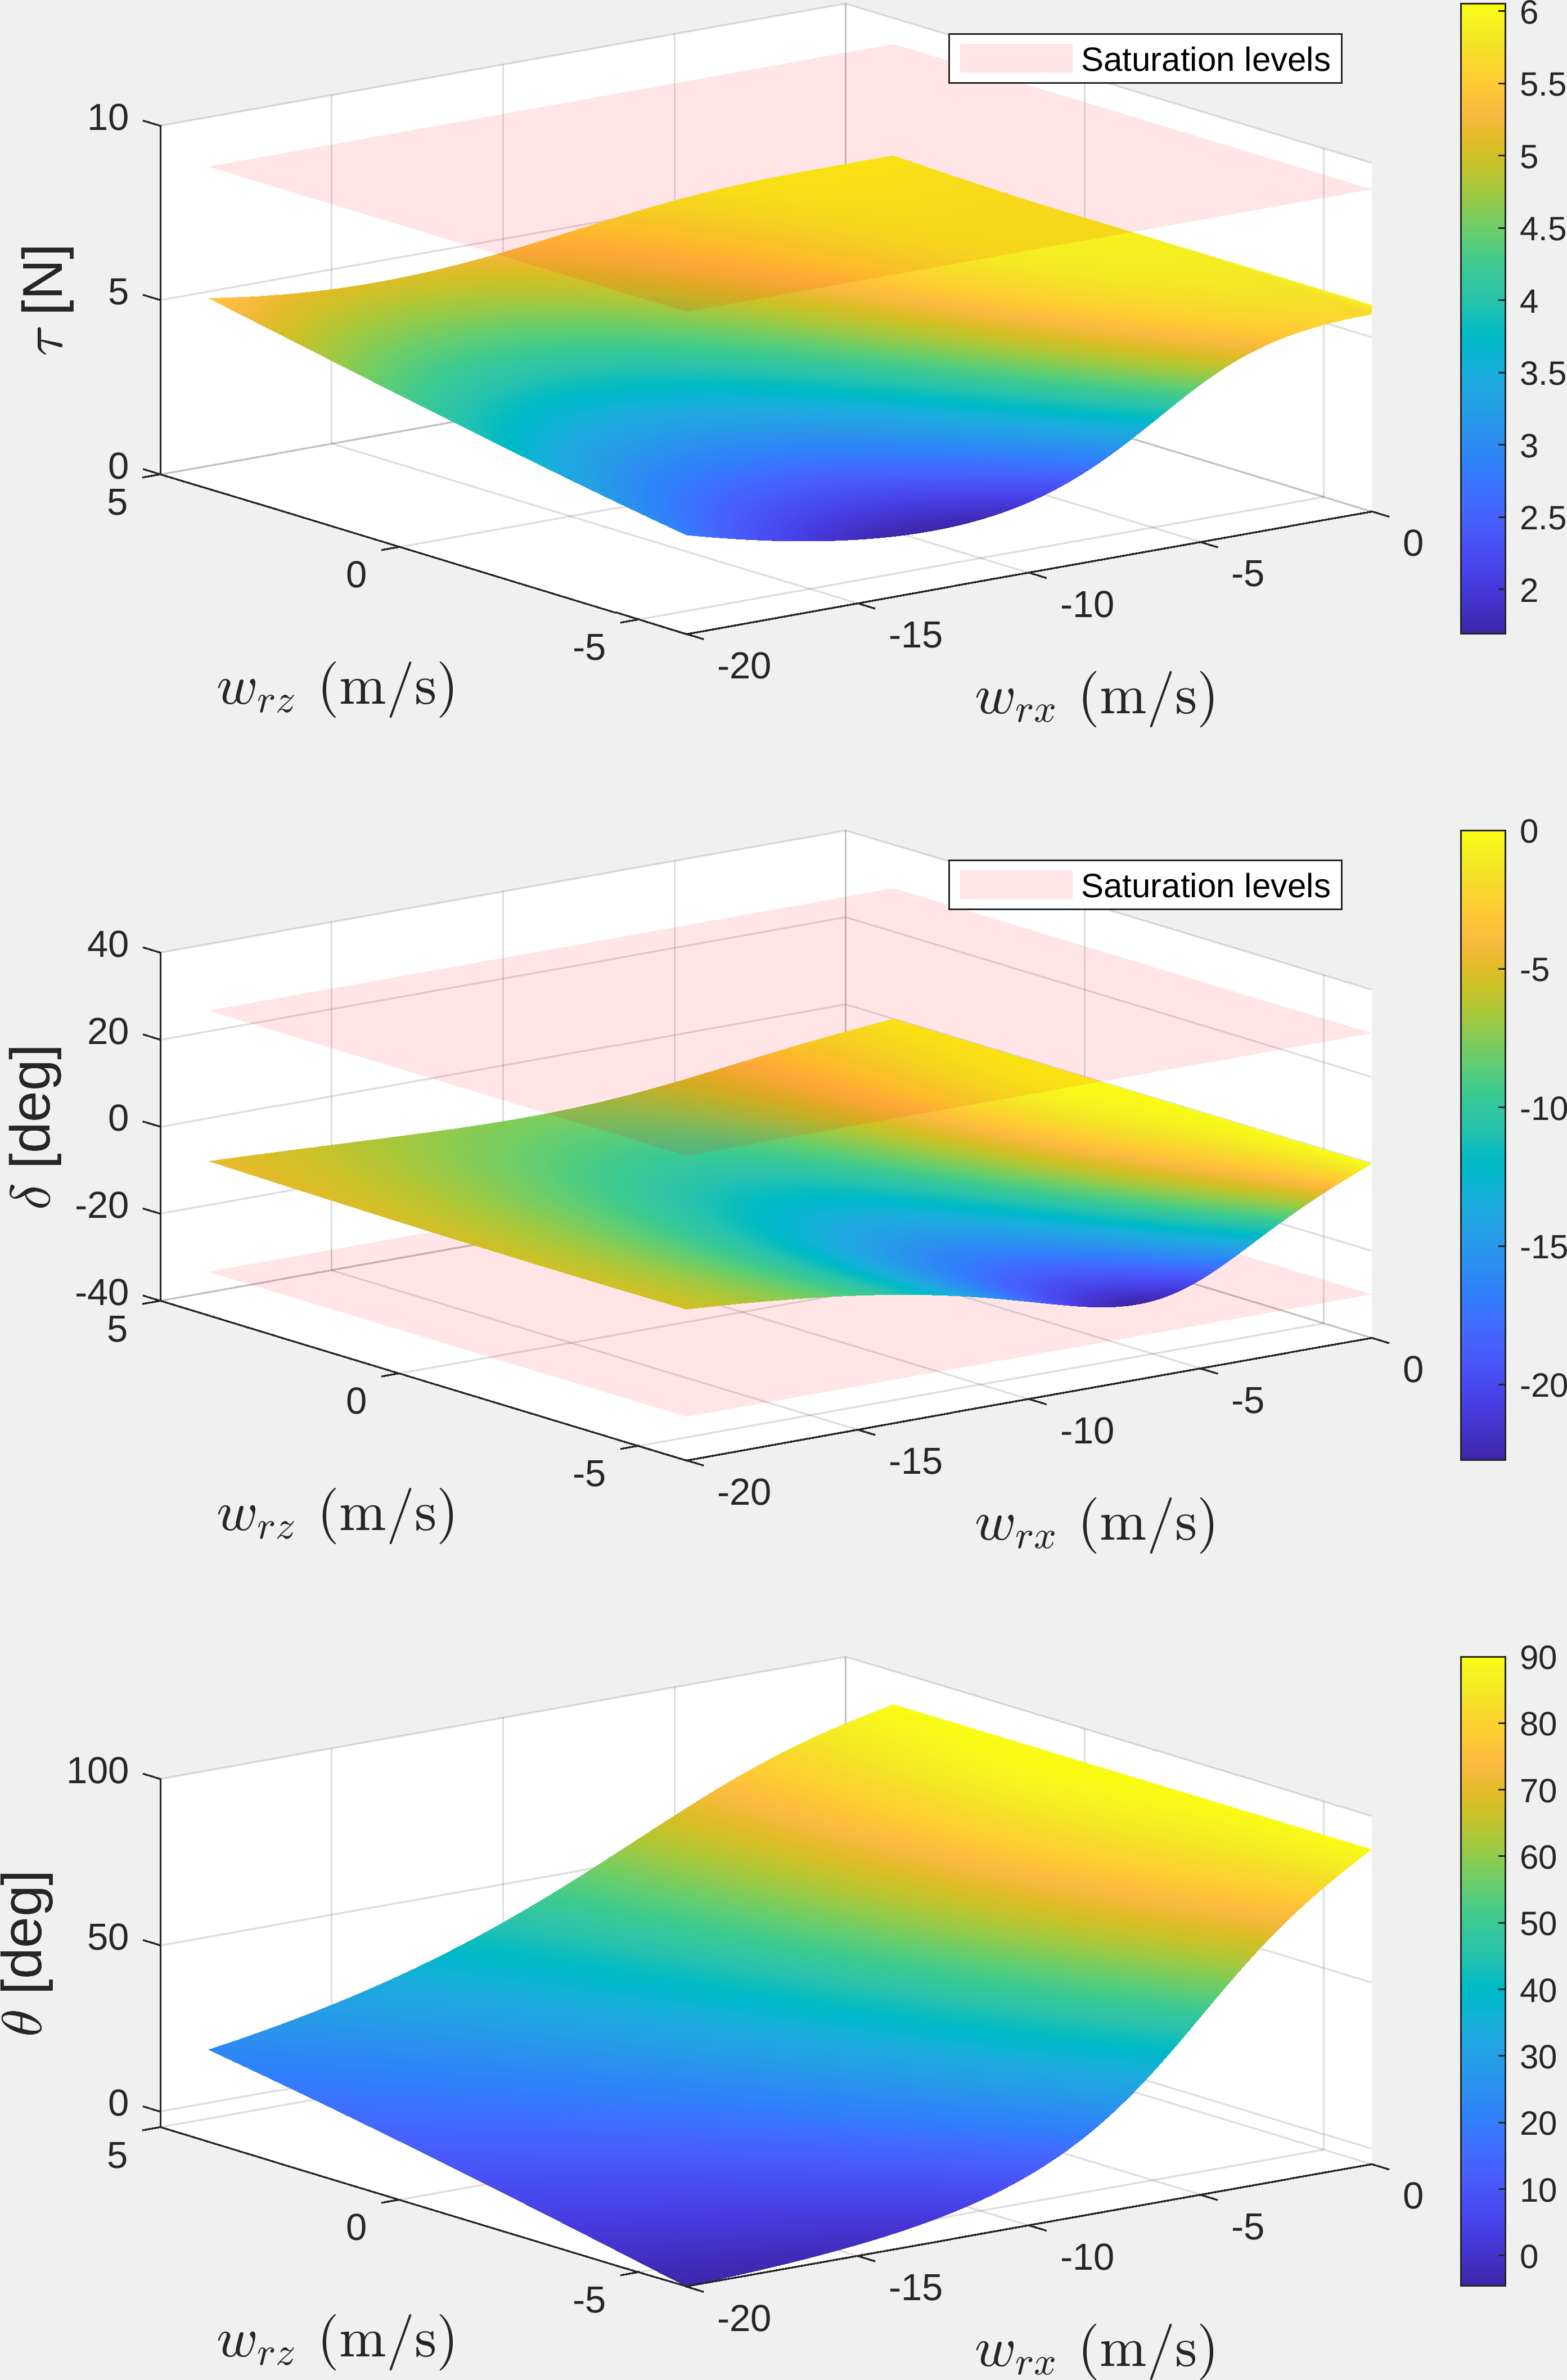
\includegraphics[trim=0cm 0cm 0cm 0cm,clip,width=0.5\columnwidth]{figures/equilibrium_wx_wz.png}
        \caption{Les paramètres ($\tau$, $\delta$, $\theta$) de l'ensemble des points d'équilibres (surface) obtenue à l'aide du Théorème~\ref{thm:eqs} et de l'Algorithme \ref{alg:eq} pour un vent constant horizontal et vertical ($w_{\text{r}x}$,$w_{\text{r}z}$), avec les saturations des actionneurs (rose).}
        \label{fig:saturation}
    \end{figure}
    Il est possible de faire une coupe des surfaces présentée dans \eqref{fig:saturation} pour une vitesse verticale nulle $\boldsymbol{w}_{\text{rx}} = 0$, ce qui nous donne le résultat de la Figure \ref{fig:saturation_wz0}
    \begin{figure}[ht!]
        \centering
        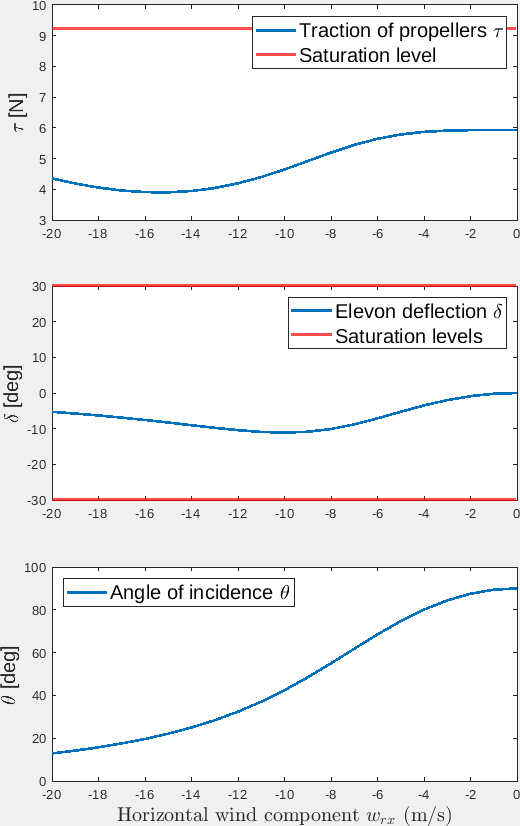
\includegraphics[trim=0cm 0cm 0cm 0cm,clip,width=0.5\columnwidth]{figures/equilibrium.png}
        \caption{Section des surfaces de la Figure \ref{fig:saturation} pour $w_{\text{r}z} = \SI{0}{\meter\per\second}$.}
        \label{fig:saturation_wz0}
    \end{figure}

\section{Dynamiques linéarisés}
\subsection{Dynamique linéarisé sans vent}
Considérons le cas sans vent discuté dans la section \ref{sec:eq_nowind} pour lequel nous utilisons le vecteur de commande $\boldsymbol{u}_{\text{nowind}}$  et le vecteur de commande à l'équilibre $\boldsymbol{u}_{\text{nowind},\text{eq}}$ défini dans l'équation \eqref{eq:bar_u} et rappelons la transformation du vecteur de commande suivante $ \boldsymbol{u}_{\text{nowind}} := \begin{bmatrix}\tau_{1}  \!&\! \tau_{2}  \!&\! \delta_{1}\tau_{1} \!&\! \delta_{2}\tau_{2} \end{bmatrix}^\top$, la dynamique linéarisé dans le cas sans vent est 
\begin{align}
    \label{eq:linearized}
     \boldsymbol{\dot{\tilde{x}}} = \boldsymbol{A}_{0} \tilde{\boldsymbol{x}} + \boldsymbol{G}_{0} (\boldsymbol{u}_{\text{nowind}}-\boldsymbol{u}_{\text{nowind},\text{eq}}),
\end{align}
où l'expression de $\boldsymbol{A}_{0}$ est
\begin{align}
    \label{matrice_A}
        \boldsymbol{A}_{0} = \boldsymbol{A}_{w} \Big|_{\boldsymbol{w}=0} =\begin{bmatrix}
        \mathbb{0}_{3} & \mathbb{I}_{3} & \mathbb{0}_{3} & \mathbb{0}_{3} \\
        \mathbb{0}_{3} & \mathbb{0}_{3} &  \boldsymbol{A}_{v\epsilon} & \mathbb{0}_{3} \\
        \mathbb{0}_{3} & \mathbb{0}_{3} & \mathbb{0}_{3} & \boldsymbol{A}_{\epsilon\omega} \\
        \mathbb{0}_{3} & \mathbb{0}_{3} & \mathbb{0}_{3} & \mathbb{0}_{3}
        \end{bmatrix},
\end{align}
avec les matrices suivantes
\begin{align*}
    \boldsymbol{A}_{\epsilon\omega} = \frac{\sqrt{2}}{4}\begin{bmatrix} 
        1 & 0 & -1 \\ 
        0 & 1 & 0  \\
       1 & 0 & 1
    \end{bmatrix} \text{ et } \boldsymbol{A}_{ v\epsilon} = \sqrt{2}\begin{bmatrix} 
        0 & -2g & 0\\
        g & 0 & g  \\ 
         0 & -2g & 0 \end{bmatrix},
\end{align*}
alors que l'expression de $\boldsymbol{G}_{0}$ est
\begin{align*}
    \boldsymbol{G}_{0}  := \begin{bmatrix}
    \mathbb{0}_{3\times 1} & \mathbb{0}_{3\times 1} & \mathbb{0}_{3\times 1} & \mathbb{0}_{3\times 1}\\
    0 & 0 & a_{\text{g}} & a_{\text{g}}\\
    0 & 0 & 0 & 0\\
    b_{\text{g}} & b_{\text{g}}  & 0 & 0\\
    \mathbb{0}_{3\times 1} & \mathbb{0}_{3\times 1} & \mathbb{0}_{3\times 1} & \mathbb{0}_{3\times 1}\\
    c_{\text{g}} & -c_{\text{g}} & d_{\text{g}} & -d_{\text{g}}\\
    0 & 0 & e_{\text{g}} & e_{\text{g}}\\
    f_{\text{g}} & -f_{\text{g}} & 0 & 0\\
    \end{bmatrix} , 
\end{align*}
avec
\begin{align*}
    \left[\!\! \begin{array}{c|c} 
    a_{\text{g}} & b_{\text{g}} \\ \hline
    c_{\text{g}} & d_{\text{g}} \\ \hline
    e_{\text{g}} & f_{\text{g}}
    \end{array} \!\!\right] \!=\!
    \left[\begin{array}{c|c}
   \shortminus \frac{S_{\text{wet}}}{4mS_{\text{p}}}C_{\ell}\xi_{\text{f}}  & \frac{1}{m}( 1-\frac{S_{\text{wet}}}{2S_{\text{p}}} C_{\text{d}}) \\ \hline
    \frac{k_{\text{m}} }{J_{x}k_{\text{f}}}  &   \! \frac{ S_{\text{wet}} a_{y} }{4 J_{x} S_{\text{p}} } C_{\ell}\xi_{\text{f}} \!\\ \hline
    \!\! \frac{S_{\text{wet}}\Delta_{\text{r}}}{4J_{y}S_{\text{p}}} C_{\ell}\xi_{\text{m}} \!\! & 
    \frac{1}{J_{z}}(p_{y}\!+\!\frac{S_{\text{wet}}}{4S_{\text{p}}} a_{y} C_{\text{d}})\!\!
    \end{array}\right].
\end{align*}

\subsection{Dynamique linéarisé en présence de vent}

Pour chacun des équilibres caractérisés dans le Théorème~\ref{thm:eqs}, nous détaillons les équations linéarisées du mouvement par rapport au modèle non linéaire simplifié à faible vitesse \eqref{eq:dyna_simp}. Une approche directe conduirait à des équations linéarisées qui dépendent de l'angle $\psi$ caractérisé à l'étape 1 de l'Algorithme~\ref{alg:eq}. Au lieu de cela, nous définissons ici les coordonnées incrémentales dans un cadre de référence inertiel convenablement tourné, de sorte que la dynamique linéarisée soit indépendante de l'angle $\psi$.
Plus précisément, pour chaque condition de vent d'équilibre $\boldsymbol{w}_{\text{eq}}$ associé à l'équilibre $(\boldsymbol{u}_{\text{eq}}, \boldsymbol{p}_{\text{eq}},\boldsymbol{v}_{\text{eq}}, \boldsymbol{q}_{\text{eq}},\boldsymbol{\omega}_{\text{b},\text{eq}})$  caractérisé en \eqref{eq:qpsi}--\eqref{eq:qtheta}, 
désignant les composantes scalaire et vectorielle du quaternion en \eqref{eq:qeq} comme
$\boldsymbol{q}_{\text{eq}} = (\eta_{\text{eq}}, \boldsymbol{\epsilon}_{\text{eq}})$, et à partir de la matrice de rotation
$\boldsymbol{R}_{\psi} :=    \boldsymbol{R}(\boldsymbol{q}_{\mathrm{eq}\psi})$ introduite au début de la preuve du Théorème~\ref{thm:eqs}, nous étudions ici la dynamique incrémental linéaire du vecteur d'état tourné :  
\begin{align}
\label{eq:xtilde}
     \nonumber &\tilde{\boldsymbol{x}} := (\tilde{\boldsymbol{p}},
     \tilde{\boldsymbol{v}},
     \tilde{\boldsymbol{\epsilon}},
     \tilde{\boldsymbol{\omega}}_{\text{b}}) = \left(\boldsymbol{R}^\top_{\psi} (\boldsymbol{p} \! \shortminus \! \boldsymbol{p}_{\text{eq}}), \boldsymbol{R}^\top_{\psi} \boldsymbol{v}, \boldsymbol{R}^\top_{\psi} (\boldsymbol{\epsilon} \! \shortminus \! \boldsymbol{\epsilon}_{\text{eq}}), \boldsymbol{\omega}_{\text{b}} \right), \\ &\tilde{\boldsymbol{u}} := \boldsymbol{u}-\boldsymbol{u_{\text{eq}}}, \quad \tilde{\boldsymbol{w}} := \boldsymbol{R}^\top_{\psi} (\boldsymbol{w}-\boldsymbol{w}_{\mathrm{eq}}).
\end{align}
Notez que la rotation en \eqref{eq:xtilde} possède la propriété $\boldsymbol{R}^\top_{\psi} \boldsymbol{\epsilon}_{\text{eq}} = \smallmat{0 & \sin(\frac{\theta}{2}) & 0}^\top$, ce qui simplifie grandement le mouvement linéarisé.

En exploitant le fait que les vitesses lineaaire et angulaire ($\boldsymbol{v}_{\text{eq}}$, $\boldsymbol{\omega}_{\text{b,eq}})$ doit être nulle à l'équilibre (voir \eqref{eq:equilibrium}), nous prouvons ci-dessous que la dynamique linéarisée de l'état \eqref{eq:xtilde} est donnée par
\begin{align}
\label{eq:lpv_linearisation}
 \boldsymbol{\dot{\tilde{x}}} &= \boldsymbol{A}_{w} \tilde{\boldsymbol{x}} + \boldsymbol{G}_{w} \tilde{\boldsymbol{u}} + \boldsymbol{E}_{w}  \tilde{\boldsymbol{w}} \\
 &= \smallmat{
     \mathbb{0}_{3} & \mathbb{I}_{3} & \mathbb{0}_{3} &\mathbb{0}_{3} \\
    \mathbb{0}_{3} & \boldsymbol{A}_{vv}  & \boldsymbol{A}_{v\epsilon}  & \mathbb{0}_{3}\\
    \mathbb{0}_{3} & \mathbb{0}_{3} & \mathbb{0}_{3} & \boldsymbol{A}_{\epsilon \omega} \\    
    \mathbb{0}_{3} & \mathbb{0}_{3} &  \boldsymbol{A}_{\omega \epsilon} & \mathbb{0}_{3}
    } \tilde{\boldsymbol{x}} \!+\!
    \smallmat{ \mathbb{0}_{3 \times 4} \\
     \boldsymbol{G}_{v}\\
     \mathbb{0}_{3 \times 4}\\
     \boldsymbol{G}_{\omega}
    } \tilde{\boldsymbol{u}}
    \!+\! \smallmat{
     \mathbb{0}_{3 \times 3} \\
     \boldsymbol{E}_{v} \\
     \mathbb{0}_{3 \times 3} \\
     \boldsymbol{E}_{\omega} 
     } \!\tilde{\boldsymbol{w}},
     \nonumber
\end{align}
%
avec les matrices $\boldsymbol{A}_{vv} $, $\boldsymbol{A}_{v\epsilon}$, $\boldsymbol{A}_{\epsilon \omega_{\text{b}}}$, $\boldsymbol{A}_{\omega \epsilon}$, $ \boldsymbol{G}_{v}$, $\boldsymbol{G}_{\omega}$ $\boldsymbol{E}_{v}$, $\boldsymbol{E}_{\omega}$ construite en suivant l'Algorithme~\ref{alg:linea}.

\begin{theorem} \label{th:lin}
Pour tout vent constant, $\boldsymbol{w} =\smallmat{w_x & w_y & w_z}^\top \in \real^3$ ayant une composante horizontale non nulle $\smallmat{w_x \\ w_y}$, et le doublet d'équilibre qui découle $(\boldsymbol{u}_{\text{eq}}, \boldsymbol{x}_{\text{eq}})$ de la dynamique \eqref{eq:dyna_simp}, tels que caractérisés dans \eqref{eq:qpsi}-\eqref{eq:qtheta}, la dynamique linéarisée du vecteur état incrémental \eqref{eq:xtilde} est donné par \eqref{eq:lpv_linearisation} avec les matrices construites comme dans l'Algorithme~\ref{alg:linea}.
\end{theorem}
%
\begin{proof}
Tout d'abord, en exploitant la matrice de rotation 
$\boldsymbol{R}_{\psi} :=    \boldsymbol{R}(\boldsymbol{q}_{\mathrm{eq}\psi})$ utilisé dans \eqref{eq:xtilde}, nous transformons la dynamique non linéaire \eqref{eq:dyna_simp} en coordonnées tournées
\begin{align}
\label{eq:rotated_coord}
(\boldsymbol{p}_{\text{r}} ,
\boldsymbol{v}_{\text{r}} ,
\boldsymbol{q}_{\text{r}}
)
:=
\left(\boldsymbol{R}_{\psi}^\top
\boldsymbol{p},
\boldsymbol{R}_{\psi}^\top \boldsymbol{v},
\boldsymbol{q}_{\mathrm{eq}\psi}^{-1} \otimes
\boldsymbol{q}
\right), 
\; \boldsymbol{w}_{\text{r}}:=\boldsymbol{R}_{\psi}^\top\boldsymbol{w}
\end{align}
où $\boldsymbol{\omega}_{\text{b}}$ reste inchangée car elle est exprimée dans le repère du corps. 
Quelques observations permettent de simplifier
la dynamique transformée \eqref{eq:dyna_simp}:
\begin{itemize}
    \item nous avons $\boldsymbol{R}_{\psi}^\top
    m\boldsymbol{g} = m\boldsymbol{g}$ car la rotation de $\psi$ est autour de l'axe $z_{[\text{i}]}$;
    \item comme $\boldsymbol{q}_{\text{r}} = \boldsymbol{q}_{\mathrm{eq}\psi}^{-1} \otimes \boldsymbol{q}$, alors $\boldsymbol{R}_{\psi}^\top \boldsymbol{R}(\boldsymbol{q}) = \boldsymbol{R}(\boldsymbol{q}_{\text{r}})$; 
    \item comme $\boldsymbol{v}_{\text{b}} := \boldsymbol{R}^\top(\boldsymbol{q}) (\boldsymbol{v}-\boldsymbol{w})$ (comme défini après l'équation \eqref{eq:Mb}), alors $\| \boldsymbol{v}_{\text{b}} \| = \| \boldsymbol{v} -  \boldsymbol{w}  \| - \| \boldsymbol{v}_{\text{r}} -  \boldsymbol{w}_{\text{r}}  \|$
    \item enfin $\boldsymbol{R}^\top(\boldsymbol{q}) \boldsymbol{w} = \boldsymbol{R}^\top\! (\boldsymbol{q}_{\text{r}}) \boldsymbol{R}_{\psi}^\top\! \boldsymbol{R}_{\psi} \boldsymbol{w}_{\text{r}}= \boldsymbol{R}^\top \!(\boldsymbol{q}_{\text{r}}) \boldsymbol{w}_{\text{r}}$.
\end{itemize} 

Sur la base des observations ci-dessus, nous pouvons dériver la version tournée des équations \eqref{eq:dyna_simp} comme étant
\begin{subequations}\label{eq:dyna_simp_rot}
    \begin{alignat}{3}
        \boldsymbol{\dot p}_{\text{r}} &=  \boldsymbol{v}_{\text{r}}, \label{eq:p_r} \\
        m \boldsymbol{\dot v}_{\mathrm{r}} &= \!\shortminus m\boldsymbol{g} \!+ \! \boldsymbol{R}(\boldsymbol{q}_{\mathrm{r}})\left(\boldsymbol{M}_{\text{f}}(\boldsymbol{u}) \! + \! \boldsymbol{D}_{\text{f}}(\boldsymbol{u}) \lVert \boldsymbol{w}_{\text{r}} \rVert \boldsymbol{R}^\top \!(\boldsymbol{q}_{\mathrm{r}}) (\boldsymbol{v}_{\mathrm{r}} \! \shortminus \! \boldsymbol{w}_{\text{r}}) \right),  \label{eq:v_r} \\
       \boldsymbol{\dot{q}}_{\text{r}} &=  \left( \frac{1}{2}\boldsymbol{q}_{\text{r}} \otimes \smallmat{0 \\ \boldsymbol{\omega}_{\text{b}}} \right),  \label{eq:q_r}\\
        \boldsymbol{J} \boldsymbol{\dot \omega}_{\text{b}} &=   \shortminus \skewsym{\boldsymbol{\omega}_{\text{b}}}\boldsymbol{J}\boldsymbol{\omega}_{\text{b}}\! + \boldsymbol{M}_{\text{m}}(\boldsymbol{u}) \! + \! \boldsymbol{D}_{\text{m}} (\boldsymbol{u}) \lVert  \boldsymbol{w}_{\text{r}} \rVert \boldsymbol{R}^\top \!(\boldsymbol{q}_{\mathrm{r}}) (\boldsymbol{v}_{\mathrm{r}} \! \shortminus \! \boldsymbol{w}_{\text{r}})  
        \label{eq:w_r}
    \end{alignat}
\end{subequations}
Avec ces nouvelles coordonnées, les vecteurs d'état incrémental \eqref{eq:xtilde} peut être exprimés comme étant
\begin{align}
\label{eq:xtilde_rot}
     \nonumber &\tilde{\boldsymbol{x}} = \left(
     \boldsymbol{p}_{\text{r}} \! \shortminus \!  \boldsymbol{R}^\top_{\psi}\boldsymbol{p}_{\text{eq}}, \boldsymbol{v}_{\text{r}},  
     \boldsymbol{\epsilon}_{\text{r}} \! \shortminus \! \boldsymbol{R}^\top_{\psi}\boldsymbol{\epsilon}_{\text{eq}}, \boldsymbol{\omega}_{\text{b}} \right), \\ &\tilde{\boldsymbol{u}} := \boldsymbol{u}-\boldsymbol{u_{\text{eq}}}, \quad \tilde{\boldsymbol{w}} :=  \boldsymbol{w}_{\mathrm{r}}-\boldsymbol{w}_{\mathrm{r,eq}}
\end{align}
où $\boldsymbol{w}_{\mathrm{r,eq}} = \boldsymbol{R}^\top_{\psi}\boldsymbol{w}_{\mathrm{eq}} = \smallmat{w_{\text{r}x} \\ 0 \\w_{\text{r}z}}$, déjà défini dans \eqref{eq:wh}, et $\boldsymbol{R}^\top_{\psi} \boldsymbol{\epsilon}_{\text{eq}} = \smallmat{0 & \sin(\frac{\theta}{2}) & 0}^\top$ ont tous deux une structure peu dense intéressante.


En se concentrant sur la dynamique tournée \eqref{eq:dyna_simp_rot} et l'expression \eqref{eq:xtilde_rot} des variables incrémentales, la preuve du théorème revient à montrer que la linéarisation de \eqref{eq:dyna_simp_rot} autour de
l'équilibre tourné
\begin{align}
\label{eq:rotated_eq}
\boldsymbol{x}_{\text{r,eq}} &= \left( \boldsymbol{p}_{\text{r,eq}}, \boldsymbol{v}_{\text{r,eq}},
\boldsymbol{\epsilon}_{\text{r,eq}},
\boldsymbol{\omega}_{\text{br,eq}} \right) \\
\nonumber
&= \left(\boldsymbol{R}^\top_{\psi} \boldsymbol{p}_{\text{eq}},  
\smallmat{0 \\ 0 \\ 0},   \smallmat{0 \\ \sin(\frac{\theta}{2}) \\ 0}, 
\smallmat{0 \\ 0 \\ 0} \right),\;
\boldsymbol{w}_{\mathrm{r,eq}}  = \smallmat{w_{\text{r}x} \\ 0 \\w_{\text{r}z}}
\end{align}
coïncide avec l'équation \eqref{eq:lpv_linearisation} et les expressions de l'Algorithme~\ref{alg:linea}.

Dans ce but, inspirée par \cite[Proof of Lemma 1]{tregouetHal-01760720}, pour linéariser la dynamique du quaternion $\boldsymbol{q}_{\text{r}} = \left[ \eta_{\text{r}} ~ \boldsymbol{\epsilon}_{\text{r}}^\top \right]^\top$ évoluant dans ${\mathbb S}^3$, nous remplaçons  $\eta_{\text{r}}$ par sa valeur positive lié à la norme unitaire du quaternion. Ainsi, $\eta_{\text{r}} = (1- \boldsymbol{\epsilon}_{\text{r}}^\top \boldsymbol{\epsilon}_{\text{r}})^\frac{1}{2}$.
Concentrons-nous d'abord sur la matrice $\boldsymbol{A}_w$ dans \eqref{eq:lpv_linearisation}. Les trois premières lignes sont simplement $\smallmat{\mathbb{0}_{3} & \mathbb{I}_{3} & \mathbb{0}_{3} &\mathbb{0}_{3}}$, du fait de la linéarité de l'équation \eqref{eq:p_r}. 
Pour le second bloc de ligne, nous nous concentrons sur l'équation \eqref{eq:v_r} et nous commençons par caractériser $\boldsymbol{R}(\boldsymbol{q}_{\mathrm{r,eq}})$, dont la structure est relativement vide de $\boldsymbol{\epsilon}_{\text{r,eq}}$. En particulier, nous rappelons dans \eqref{eq:wb} en utilisant l'expression $\boldsymbol{R}$ dans \eqref{eq:matrix_rot}, nous pouvons écrire
\begin{align*}
    \boldsymbol{R}(\boldsymbol{q}_{\mathrm{r,eq}\textbf{}})= \boldsymbol{R}_\theta :=
     \begin{bmatrix}1-2\overline \epsilon_{2}^{2} & 0 & 2\overline\epsilon_{2} \overline{\eta} \\ 0 & 1 & 0 \\ -2\overline\epsilon_{2} \overline{\eta} & 0 & 1-2\overline\epsilon_{2}^{2} \end{bmatrix}
    = \smallmat{ \cos \theta & 0 & \sin \theta \\ 0 & 1 & 0 \\ -\sin \theta & 0 & \cos \theta },
\end{align*}
où $\overline \epsilon_{2} = \sin{\frac{\theta}{2}}$ représente le deuxième élément de $\boldsymbol{\epsilon}_{\text{r,eq}}$ selon \eqref{eq:rotated_eq} et $ \overline{\eta} = \sqrt{1-\overline \epsilon_{2}^{2}} = \cos{\frac{\theta}{2}}$.

Avec cette expression de $ \boldsymbol{R}_\theta$, nous pouvons dériver l'expression de \eqref{eq:v_r}, en utilisant la notation abrégée $\left. \cdot \right|_{\text{eq}}$ pour caractériser l'évaluation d'une fonction (matricielle ou vectorielle) à l'équilibre \eqref{eq:rotated_eq},
\begin{align}
\nonumber
\boldsymbol{A}_{vv} &\!=\! \frac{\partial }{\partial \boldsymbol{v}}  \left. \left( \frac{1}{m} \boldsymbol{R}(\boldsymbol{q}_{\text{r}}) \left( %\boldsymbol{M}_{\text{f}}(\boldsymbol{u}) +  
\boldsymbol{D}_{\text{f}}(\boldsymbol{u}) \lVert \boldsymbol{w}_{\text{r}} \rVert \boldsymbol{R}^\top \!(\boldsymbol{q}_{\mathrm{r}}) ( \boldsymbol{v}_{\mathrm{r}} \! \shortminus \! \boldsymbol{w}_{\text{r}})  \right) \right)\right|_{\text{eq}}\\
&\!=\!  \left. \frac{\partial }{\partial \boldsymbol{v}} \left( \frac{1}{m}  \boldsymbol{R}_\theta  \boldsymbol{D}_{\text{f}}(\boldsymbol{u_{\text{eq}}}) \lVert \boldsymbol{w}_{\mathrm{eq}} \rVert   \boldsymbol{R}_\theta^\top  \boldsymbol{v}_{\mathrm{r}} \right) \right|_{\text{eq}},
\label{eq:Avv_derivation}
\end{align} 
qui, compte tenu de l'égalité $\boldsymbol{D}_{\text{f,eq}} = \boldsymbol{D}_{\text{f}}(\boldsymbol{u_{\text{eq}}})$, il est facile de montrer qu'elle coïncide avec la matrice
$\boldsymbol{A}_{vv}$ donnée en \eqref{eq:Avv_alg2} dans l'Algorithme~\ref{alg:linea}.

Nous nous concentrons maintenant sur $\boldsymbol{A}_{v\epsilon}$ de la matrice 
$\boldsymbol{A}_{w}$,  qui doit être calculée à partir de \eqref{eq:v_r} de manière similaire à
\eqref{eq:Avv_derivation}, comme
\begin{align}
\boldsymbol{A}_{v\epsilon} &\!=\! \frac{\partial }{\partial \boldsymbol{\epsilon}}  \left. \left( \frac{1}{m} \boldsymbol{R}(\boldsymbol{q}_{\text{r}}) \left( 
\boldsymbol{M}_{\text{f}}(\boldsymbol{u}) +  
\boldsymbol{D}_{\text{f}}(\boldsymbol{u}) \lVert \boldsymbol{w}_{\text{r}} \rVert \boldsymbol{R}^\top \!(\boldsymbol{q}_{\mathrm{r}}) \boldsymbol{w}_{\text{r}}  \right) \right)\right|_{\text{eq}}.
\label{eq:Aveps_derivation}
\end{align} 
Pour évaluer la partie droite de \eqref{eq:Aveps_derivation}, nous demmarons de l'expression de $\boldsymbol{R}(\boldsymbol{q}) = \boldsymbol{R}\left( \smallmat{\eta \\ \epsilon}\right)$ dans \eqref{eq:matrix_rot}, après la substitution de 
$\eta = \sqrt{1-\boldsymbol{\epsilon}^\top \boldsymbol{\epsilon}} \neq 0$
(nous rappelons que pour tous les équilibres caractérisés, nous avons $\eta \neq 0$), nous pouvons calculer la dérivée généralisée
\begin{align}
\label{eq:diffR_eps}
&\partial \boldsymbol{R}_{\boldsymbol{ \epsilon}} (\boldsymbol{ \epsilon},\mathfrak{v}) := \frac{\partial }{\partial \boldsymbol{\epsilon}}
\boldsymbol{R}\left(
\smallmat{\sqrt{1-\boldsymbol{\epsilon}^\top \boldsymbol{\epsilon}} \\ \boldsymbol{\epsilon}}
\right) \mathfrak{v}  \\
\nonumber
&\; = 2 \eta \skewsym{\mathfrak{v}} \left( \frac{\boldsymbol{\epsilon}\boldsymbol{\epsilon}^\top}{1-\boldsymbol{\epsilon}^\top \boldsymbol{\epsilon}} - \mathbb{I}_{3}  \right) \shortminus 4 \mathfrak{v} \boldsymbol{\epsilon}^\top \! + \!2\boldsymbol{\epsilon} \mathfrak{v}^\top \!+ \! 2\boldsymbol{\epsilon}^\top \mathfrak{v} \mathbb{I}_{3},
\end{align}
qui implique donc
\begin{align}
\label{eq:diffRtop}
    \frac{\partial }{\partial \boldsymbol{\epsilon}}
\boldsymbol{R}^\top\left(
\smallmat{\eta \\ \boldsymbol{\epsilon}}
\right) \mathfrak{v} =
    \frac{\partial }{\partial \boldsymbol{\epsilon}}
\boldsymbol{R}\left(
\smallmat{\sqrt{1-\boldsymbol{\epsilon}^\top \boldsymbol{\epsilon}} \\ -\boldsymbol{\epsilon}}
\right) \mathfrak{v} = \partial \boldsymbol{R}_{\boldsymbol{ \epsilon}} (\boldsymbol{ -\epsilon},\mathfrak{v}).
\end{align}
Pour évaluer \eqref{eq:Aveps_derivation}, il sera utile de dériver la forme simplifiée suivante
\begin{align}
\label{eq:diffRsparse}
    &\partial \boldsymbol{R}_{\boldsymbol{ \epsilon}} \left(
    \smallmat{0 \\ \epsilon_2 \\ 0}
    ,\smallmat{\mathfrak{v}_1 \\ 0 \\ \mathfrak{v}_3}\right) \nonumber \\ 
    & = 2  \smallmat{0 & \left( \overline{\eta} - \frac{\overline \epsilon_{2}^{2}}{\overline{\eta}} \right) \mathfrak{v}_3 & 0\\
    -\overline{\eta} \mathfrak{v}_3 & 0 & \overline{\eta} \mathfrak{v}_1 \\
    0 & \left( \frac{\overline \epsilon_{2}^{2}}{\overline{\eta}} - \overline{\eta} \right) \mathfrak{v}_1 & 0} + 2\overline \epsilon_{2}\smallmat{ 0 & -2\mathfrak{v}_1 & 0\\
    \mathfrak{v}_1 & 0 & \mathfrak{v}_3 \\
    0 & -2\mathfrak{v}_3 & 0}.
\end{align}

Nous pouvons définir deux forces $(f_{\text{d}} , f_{\ell})$ qui agissent sur le drone à l'équilibre, exprimées dans le repère corps, et qui dépendent du vent $\boldsymbol{w}$ et des deux entrées similaires des élevons $\delta$. Ces deux forces sont la traînée et la portance générées par l'écoulement de l'air sur l'aile. Elles résultent du développement de l'expression $ \boldsymbol{D}_{\text{f}}(\boldsymbol{u}) \lVert \boldsymbol{v}_{\text{b}} \rVert \boldsymbol{v}_{\text{b}}$ provenant \eqref{eq:v_r} avec $\boldsymbol{D}_{\text{f}}(\boldsymbol{u})$ De \eqref{eq:df}:
\begin{align}
\label{eq:draglift}
    \smallmat{f_{\text{d}} \\ 0 \\ f_{\ell}} = - \boldsymbol{D}_{\text{f}}(\boldsymbol{u_{\text{eq}}}) \lVert \boldsymbol{w}_{\mathrm{eq}} \rVert  \boldsymbol{R}_\theta^\top \boldsymbol{w}_{\mathrm{r,eq}},
\end{align}
qui après calcul coïncide avec l'expression \eqref{eq:draglift_ALG} donner dans l'Algorithme~\ref{alg:linea}. 

À partir des deux forces $(f_{\text{d}} , f_{\ell})$ dans \eqref{eq:draglift}, il est possible de déterminer leurs dérivées partielles par rapport à la composante $\overline \epsilon_2$ du quaternion, qui représente le tangage du drone. En utilisant \eqref{eq:diffRtop}, nous obtenons
\begin{align}
    \smallmat{\frac{\partial  f_{\text{d}}  }{\partial \epsilon_{2}} \\ 0 \\ \frac{\partial  f_{\ell}  }{\partial \epsilon_{2}}} = - \boldsymbol{D}_{\text{f}}(\boldsymbol{u_{\text{eq}}})  \lVert \boldsymbol{w}_{\mathrm{eq}} \rVert \partial \boldsymbol{R}_{\boldsymbol{ \epsilon}}( -\boldsymbol{ \epsilon}, \boldsymbol{w}_{\mathrm{r,eq}}) \smallmat{0\\ 1\\ 0},
\end{align}
qui après calcul en utilisant l'égalité $\boldsymbol{D}_{\text{f,eq}} = \boldsymbol{D}_{\text{f}}(\boldsymbol{u_{\text{eq}}})$,
coïncide avec l'équation \eqref{eq:draglift_ALG}, donné dans l'Algorithme~\ref{alg:linea}.

En suivant des calculs similaires,  la force
$f_{\text{m}}$ générée par les moteurs, liée à la traction des hélices et à la traînée générée par l'écoulement de l'air sur l'aile, et la force $f_{\text{e}}$ générée par les élevons, liée à l'écoulement de l'air créé par les hélices, sont obtenues à partir de \eqref{eq:Mf} sont défini par 
\begin{align}
\label{eq:motor_el}
    \smallmat{ f_{\text{m}}  \\ 0 \\ f_{\text{e}} } &= \boldsymbol{M}_{\text{f}}(\boldsymbol{u_{\text{eq}}}) ,
\end{align}
qui, après calculs, coïncident avec les sélections de \eqref{eq:motor_elevon_forces}, données dans l'Algorithme~\ref{alg:linea}.

En utilisant les définitions \eqref{eq:diffR_eps}, \eqref{eq:diffRtop}, ainsi que les expressions \eqref{eq:diffRsparse}, \eqref{eq:draglift}, \eqref{eq:motor_el}, et leurs formes équivalentes indiquées dans \eqref{eq:draglift_ALG}, \eqref{eq:motor_elevon_forces} données dans l'Algorithme~\ref{alg:linea}, nous pouvons finalement calculer à partir de \eqref{eq:Aveps_derivation}
\begin{multline*}
    \!\boldsymbol{A}_{v\epsilon} \!=\! \frac{1}{m} \big( \partial \boldsymbol{R}_{\boldsymbol{ \epsilon}} (\boldsymbol{ \epsilon} , \boldsymbol{M}_{\text{f}}(\boldsymbol{u_{\text{eq}}}))  \shortminus \partial \boldsymbol{R}_{\boldsymbol{ \epsilon}} ( \boldsymbol{ \epsilon} ,\boldsymbol{D}_{\text{f}}(\boldsymbol{u_{\text{eq}}})  \lVert \boldsymbol{w}_{\mathrm{eq}} \rVert  \boldsymbol{R}_\theta^\top \! \boldsymbol{w}_{\mathrm{eq}})  \\    \left. \shortminus  \boldsymbol{R}_\theta \boldsymbol{D}_{\text{f}}(\boldsymbol{u})  \lVert \boldsymbol{w}_{\mathrm{r,eq}} \rVert \partial \boldsymbol{R}_{\boldsymbol{ \epsilon}}( -\boldsymbol{ \epsilon}, \boldsymbol{w}_{\mathrm{r,eq}})\smallmat{0\\ 1\\ 0} \big)\right|_{\mathrm{eq}}.
\end{multline*}
qui fournit l'expression \eqref{eq:Aveps_derivation_ALG} dans l'Algorithme~\ref{alg:linea} après quelques calculs exploitant également $\boldsymbol{D}_{text{f,eq}} = \boldsymbol{D}_{text{f}}(\boldsymbol{u_{\text{eq}}})$.

Nous nous concentrons maintenant sur la matrice $\boldsymbol{A}_{\epsilon \omega}$ de  $\boldsymbol{A}_{w}$, et nous rappelons que, en raison des propriétés du produit de quaternion (voir, par exemple, \cite{hamel_minhduc}), 
$\smallmat{\eta \\ \boldsymbol{\epsilon}} \otimes \smallmat{0 \\ 
\boldsymbol{\omega}_{\mathrm{b}}} = 
\smallmat{ - \boldsymbol{\epsilon}^\top  \\ 
\eta \mathbb{I}_{3}   + [ \boldsymbol{\epsilon}]_{\times} 
} \boldsymbol{\omega}_{\mathrm{b}}$. 
À partir des deux termes inférieurs de la matrice du côté droit de cette dernière équation, en développant \eqref{eq:q_r}
et en calculant $\boldsymbol{A}_{\epsilon \omega} = \left. \frac{\partial }{\partial \boldsymbol{\omega}_{\text{b}}} \left( \frac{1}{2} \boldsymbol{{q}}_{\text{r}}  \otimes \smallmat{0 \\ \boldsymbol{\omega}_{\text{b}}} \right) \right|_{\mathrm{eq}}$,
nous obtenons les deux termes de l'expression \eqref{eq:Aveps_derivation_ALG} donnée dans l'Algorithme~\ref{alg:linea}.

Nous nous concentrons maintenant sur la matrice $\boldsymbol{A}_{\omega \epsilon}$ de $\boldsymbol{A}_{w}$, qui doit être calculée à partir de \eqref{eq:w_r}. Comme seul le dernier terme de la partie droite dépend de $\boldsymbol{\epsilon}$ (par l'intermédiaire de $\boldsymbol{q}_{\mathrm r}$), nous obtenons

\begin{align}
\label{eq:Aomega_eps_first}
\boldsymbol{A}_{ \omega \epsilon} =  \boldsymbol{J}^{-1}
\boldsymbol{D}_{\mathrm{m}} (\boldsymbol{u}_{\text{eq}}) \lVert  \boldsymbol{w}_{\mathrm{r}} \rVert 
\left. 
\frac{\partial }{\partial \boldsymbol{\epsilon}} \left( \boldsymbol{R}^\top \!(\boldsymbol{q}_{\mathrm{r}}) (\boldsymbol{v}_{\mathrm{r}} \! \shortminus \! \boldsymbol{w}_{\text{r}}) \right) \right|_{\mathrm{eq}}.
\end{align}
Pour calculer l'expression explicite de \eqref{eq:Aomega_eps_first}, nous exploitons à nouveau \eqref{eq:diffRtop} et \eqref{eq:diffRsparse}, et utilisons l'expression de $\boldsymbol{D}_{\mathrm{m}}$ dans \eqref{eq:dm}, ainsi que les identités $\overline \eta^2 - \overline \epsilon_2^2 = \cos \theta$ et $2\overline \eta \overline \epsilon_2^2 = \sin \theta$, qui fournissent, après quelques simplifications, l'expression \eqref{eq:ddotomega_deps}, donnée dans l'Algorithme~\ref{alg:linea}.

Passons maintenant à la dérivation des entrées de la matrice $\boldsymbol{G}_{w}$ dans \eqref{eq:lpv_linearisation}, dont les composantes peuvent être dérivées de \eqref{eq:v_r} et \eqref{eq:w_r}. En utilisant les quatre entrées de $\boldsymbol{u}$ dans \eqref{eq:vector_u}, et en se basant également sur la structure de $\boldsymbol{M}_{\text{f}}$,
$\boldsymbol{D}_{\text{f}}$, dans \eqref{eq:Mf}, \eqref{eq:df}, la forme explicite pour
\begin{align}
    \boldsymbol{G}_{v} \! &= \! 
    \frac{1}{m} \boldsymbol{R}_\theta \! \left.\frac{\partial}{\partial \boldsymbol{u}} \! 
     \left( \boldsymbol{M}_{\text{f}}(\boldsymbol{u}) \! - \! \boldsymbol{D}_{\text{f}}(\boldsymbol{u}) \lVert \boldsymbol{w}_{\text{r}} \rVert \boldsymbol{w}^{\text{b}}_{\mathrm{eq}}   \right)\right|_{\mathrm{eq}} ,
\end{align}
peut être calculée comme dans \eqref{eq:Gv_ALG_luca}, après quelques factorisations. 

De même, sur la base des matrices $\boldsymbol{M}_{\text{m}}$, $\boldsymbol{D}_{\text{m}}$ dans \eqref{eq:Mm}, \eqref{eq:dm}, 
nous pouvons calculer
\begin{align}
     \boldsymbol{G}_{\omega} \! &= \!  \boldsymbol{J}^{-1} \! \left.\frac{\partial}{\partial \boldsymbol{u}} \! 
     \left( \boldsymbol{M}_{\text{m}}(\boldsymbol{u}) \! - \! \boldsymbol{D}_{\text{m}}(\boldsymbol{u}) \lVert \boldsymbol{w}_{\text{r}} \rVert \boldsymbol{w}^{\text{b}}_{\mathrm{eq}}   \right)\right|_{\mathrm{eq}}
\end{align}
comme dans \eqref{eq:Gomega_ALG_Luca}, après quelques factorisations. 


Déterminons enfin l'expression de $\boldsymbol{E}_{v}$ dans \eqref{eq:lpv_linearisation}. Notons d'abord que nous pouvons écrire
$\|\boldsymbol{w}_\text{r}\| \boldsymbol{w}_\text{r} = 
 \boldsymbol{w}_\text{r} \sqrt{\boldsymbol{w}_\text{r}^\top \boldsymbol{w}_\text{r}  }$, de sorte que
$$
\frac{\partial }{\partial \boldsymbol{w}_\text{r}}
\|\boldsymbol{w}_\text{r}\| \boldsymbol{w}_\text{r} = 
\|\boldsymbol{w}_\text{r}\| \mathbb{I}_3
+ \frac{\boldsymbol{w}_\text{r} \boldsymbol{w}_\text{r}^\top}{\|\boldsymbol{w}_\text{r}\|} = 
\|\boldsymbol{w}_\text{r}\|
\left( \mathbb{I}_3 + \frac{\boldsymbol{w}_\text{r} \boldsymbol{w}_\text{r}^\top}{\boldsymbol{w}_\text{r}^\top \boldsymbol{w}_\text{r}} \right).
$$

À l'aide de \eqref{eq:v_r} et \eqref{eq:w_r} et de l'expression de $\boldsymbol{w}_\text{r}$ dans \eqref{eq:rotated_coord} et en suivant des calculs similaires aux cas précédents, nous obtenons l'expression
\eqref{eq:Ev_alg2} (indiquée dans l'Algorithme~\ref{alg:linea}), pour $\boldsymbol{E}_{v} = -  \frac{1}{m} \boldsymbol{R}_\theta \left. \frac{\partial}{\partial \boldsymbol{w}_\text{r}} \left(  \! \boldsymbol{D}_{\text{f}}(\boldsymbol{u}) \lVert \boldsymbol{w}_{\text{r}} \rVert \boldsymbol{w}_{\text{r}}  \right)\right|_{\mathrm{eq}} $ et  
 $\boldsymbol{E}_{w} = - \boldsymbol{J}^{-1} \left.
 \frac{\partial}{\partial \boldsymbol{w}_\text{r}} \left(  \boldsymbol{D}_{\text{m}}(\boldsymbol{u}) \lVert \boldsymbol{w}_{\text{r}} \rVert \boldsymbol{w}_{\text{r}}\right)\right|_{\mathrm{eq}}$, où nous rappelons que $\boldsymbol{D}_{\text{m,eq}} = \boldsymbol{D}_{\text{m}}(\boldsymbol{u_{\text{eq}}})$.
\end{proof}

\begin{algorithm}
     \caption{Détermination des matrices de la linéarisation de \eqref{eq:lpv_linearisation}}\label{alg:linea}
      \hspace*{.1cm} \textbf{Entrées} : Vecteur de vent $\boldsymbol{w}_{\text{eq}} =\smallmat{w_x & w_y & w_z}^\top$ et\\
      \hspace*{1.2cm} d'équilibre $(\boldsymbol{u}_{\text{eq}}, \boldsymbol{x}_{\text{eq}})$ provenant de \eqref{eq:equilibrium} et de l'Algorithme~\ref{alg:eq}.\\
 \hspace*{.1cm} \textbf{Sorties} : 
 Matrices $\boldsymbol{A}_{w}$, $\boldsymbol{G}_{w}$, $\boldsymbol{E}_{w}$ dans \eqref{eq:lpv_linearisation}

\begin{algorithmic}[1]

\State Sélectionner les paramètres $\psi$, $\theta$, $\tau$, $\delta$ de \eqref{eq:equilibrium} à l'aide de l'Algorithme~\ref{alg:eq} et de $\overline \epsilon_{2} = \sin{\frac{\theta}{2}}$, $\overline \eta =  \cos{\frac{\theta}{2}}$.

        
\State Avec les valeurs de \eqref{eq:wb}, \eqref{eq:df}, \eqref{eq:dm}, définissons : 
\begin{align*}
    & \boldsymbol{R}_\psi := \smallmat{ \cos \psi & \sin \psi & 0 \\ -\sin \psi & \cos \psi & 0 \\ 0 & 0 & 1 },    \quad 
      \boldsymbol{R}_\theta := \smallmat{ \cos \theta & 0 & \sin \theta \\ 0 & 1 & 0 \\ -\sin \theta & 0 & \cos \theta },         \\
     &\smallmat{w_{\text{r}x} \\ 0 \\ w_{\text{r}z}} :=  \boldsymbol{R}_\psi^\top \boldsymbol{w}_{\text{eq}}, \quad
    \smallmat{w^{\text{b}}_{x} \\ w^{\text{b}}_{z}} := \smallmat{w_{\text{r}x} \cos \theta -   w_{\text{r}z} \sin\theta \\ w_{\text{r}z} \cos \theta + w_{\text{r}x} \sin \theta }
     \\
     &\left[ \! \! \begin{array}{c|c} 
     \boldsymbol{D}_{\text{f,eq}} \! \! &  \! \! \boldsymbol{D}_{\text{m,eq}}
     \end{array} \! \!\right] \! \! := \! \! \frac{\rho S}{2} \left[\begin{array}{c|c} \! \! \begin{smallmatrix}
                \shortminus C_{\text{d}} & 0 & C_{\text{d}}\xi_{\text{f}} \delta\\
                0 & 0 & 0\\
                \shortminus C_{\ell}\xi_{\text{f}} \delta & 0 & \shortminus C_{\ell}
            \end{smallmatrix} &  \! \! \begin{smallmatrix}
                0 & 0 & 0\\
               \Delta_{\text{r}}C_{\ell}\xi_{\text{m}}\delta\ & 0 & 2\Delta_{\text{r}}C_{\ell}\\
                0 & 0 & 0
            \end{smallmatrix} \end{array} \! \!\right]
\end{align*}

\State Définissons les forces de portance et de trainé ainsi que leurs dérivées par rapport à $\epsilon_2$ (défini dans l'étape 1), comme
\begin{equation}
\label{eq:draglift_ALG}
\!\! \smallmat{\!f_{\text{d}} & \frac{\partial  f_{\text{d}}  }{\partial \epsilon_{2}} \!\! \\ 0 & 0  \\ \! f_{\ell} & \frac{\partial  f_{\ell} \!\! }{\partial \epsilon_{2}}} 
 \!\! := \! 
    \shortminus \| \boldsymbol{w}_{\mathrm{eq}} \|  \boldsymbol{D}_{\text{f,eq}}\! 
    \smallmat{\! w^{\text{b}}_{x} &  \left(\! 4 \overline{\eta}  \shortminus \frac{2\overline \epsilon_{2}^{2}}{\overline{\eta} } \! \right) w_{\text{r}z} \shortminus 8 \overline \epsilon_{2}  w_{\text{r}x} \!\! \\  0 & 0 \\  
   \! w^{\text{b}}_{z} &    \left(\! 4 \overline{\eta}  \shortminus \frac{2\overline \epsilon_{2}^{2}}{\overline{\eta} } \! \right) w_{\text{r}x} -8 \overline \epsilon_{2} w_{\text{r}z} \!\!
    }\!\!, 
\end{equation}

\State Définissons les forces des moteurs et des élevons comme
\begin{align}
\label{eq:motor_elevon_forces}
    \smallmat{ f_{\text{m}}  \\f_{\text{e}} }\! := \!\smallmat{\left(\frac{S_{\text{wet}}C_{\text{d}}}{2S_{\text{p}}}-2\right)\tau \\  - \frac{S_{\text{wet}}\tau \delta \xi_{\text{f}} C_{\ell}}{2S_{\text{p}}}}
\end{align}

\State Sélectionnons les matrices $\boldsymbol{A}_w$ dans \eqref{eq:lpv_linearisation} comme :
\begin{align}
\label{eq:Avv_alg2}
& \boldsymbol{A}_{vv} =
\frac{\| \boldsymbol{w}_{\mathrm{eq}} \| }{m} 
 \boldsymbol{R}_\theta \boldsymbol{D}_{\text{f,eq}}  \boldsymbol{R}_\theta^\top \\
\nonumber
&\smallmat{\boldsymbol{A}_{v\epsilon}^{1,2} \\ 
 \boldsymbol{A}_{v\epsilon}^{2,1} \\ \boldsymbol{A}_{v\epsilon}^{2,3} \\ \boldsymbol{A}_{v\epsilon}^{3,2}}
      := \smallmat{ 2 \overline{\eta}  - \frac{\overline \epsilon_{2}^{2}}{\overline{\eta} }  & 4 \overline \epsilon_{2} &  2\overline \epsilon_{2}^{2} -1 & 2\overline \epsilon_{2} \overline{\eta} \\
     -2 \overline{\eta}  & -2 \overline \epsilon_{2} & 0 & 0 \\ 
      2 \overline \epsilon_{2} & -2 \overline{\eta}  & 0 & 0 \\
      -4 \overline \epsilon_{2} & 2 \overline{\eta}  - \frac{\overline \epsilon_{2}^{2}}{\overline{\eta} } & -2\overline \epsilon_{2} \overline{\eta}  & 1- 2\overline \epsilon_{2}^{2}   }\smallmat{ f_{\text{e}}  + f_{\ell}  \\ f_{\text{m}}  + f_{\text{d}}  \\ \frac{\partial  f_{\text{d}}  }{\partial \overline \epsilon_{2}} \\ \frac{\partial  f_{\ell}  }{\partial \overline \epsilon_{2}}}\\
\label{eq:Aveps_derivation_ALG}
&  \boldsymbol{A}_{v\epsilon} = \frac{1}{m}\smallmat{ 
        0 & \boldsymbol{A}_{v\epsilon}^{1,2} & 0 \\ 
        \boldsymbol{A}_{v\epsilon}^{2,1} & 0 & \boldsymbol{A}_{v\epsilon}^{2,3}  \\
        0 & \boldsymbol{A}_{v\epsilon}^{3,2} & 0
   }, 
    %\label{eq:Aeomega_ALG}
   \boldsymbol{A}_{\epsilon \omega} = \frac{\overline{\eta}  }{2} \mathbb{I}_{3} + \frac{\overline \epsilon_{2}}{2}\smallmat{
        0 & 0 &  1 \\ 
        0 & 0 & 0  \\
        \shortminus 1 & 0 & 0
    }\\
\label{eq:ddotomega_deps}
&   \boldsymbol{A}_{ \omega \epsilon} = \tfrac{\rho S C_{\ell} \Delta_{\text{r}}  \lVert \boldsymbol{w}_{\mathrm{eq}} \rVert (w^{\text{b}}_{x} -  \xi_{\text{m}} \delta w^{\text{b}}_{z})}{J_{y} \overline{\eta}  } \smallmat{ 
        0 & 0 & 0 \\ 
        0 & 1  & 0  \\
       0 & 0 & 0
    }
\end{align}
\algstore{myalg}


\end{algorithmic}
\end{algorithm}

\begin{algorithm}                     
    \begin{algorithmic} [1]           
        \algrestore{myalg}
        \State Sélectionnons les matrices $\boldsymbol{G}_w$ dans \eqref{eq:lpv_linearisation} comme : 
        \begin{align}
        \nonumber
        & \boldsymbol{G}_{v} = \frac{1}{m}    \boldsymbol{R}_\theta \!\! \left[ \!\! \begin{array}{c|c} 
            \boldsymbol{G}_{v\tau}\!\! & \! \! \boldsymbol{G}_{v\delta} 
            \end{array} \!\! \right], \; \boldsymbol{G}_{v\tau} :=      \smallmat{
        1 \shortminus \frac{S_{\text{wet}} C_{\text{d}}}{4S_{\text{p}}}\\ 0 \\ \shortminus\frac{S_{\text{wet}} C_{\ell} \xi_{\text{f}}\delta}{2S_{\text{p}}} } \smallmat{ 1 \\ 1}^\top                     \\
        \label{eq:Gv_ALG_luca}
        &\quad  \boldsymbol{G}_{v\delta} := 
        \smallmat{
                -   \frac{1}{4}\rho S C_{\text{d}} \xi_{\text{f}} \lVert \boldsymbol{w}_{\text{eq}} \rVert w^{\text{b}}_{z}\\0 \\\shortminus \frac{S_{\text{wet}}  C_{\ell} \xi_{\text{f}}\tau}{2S_{\text{p}}} + \frac{1}{4}\rho S C_{\ell}  \xi_{\text{f}} \lVert \boldsymbol{w}_{\text{eq}} \rVert w^{\text{b}}_{x}
            } \smallmat{ 1 \\ 1}^\top 
        \end{align}

        \begin{align}
        \nonumber
            \boldsymbol{G}_{\omega} \! &= \!  \boldsymbol{J}^{-1} \begin{bmatrix}\boldsymbol{G}_{\omega \tau} \!\! & \!\! \boldsymbol{G}_{\omega \delta} 
            \end{bmatrix}, 
            \boldsymbol{G}_{\omega \delta} :=
            \tfrac{S_{\text{wet}}C_{\ell}\tau}{4S_{\text{p}}} 
            \smallmat{ a_{y} \xi_{\text{f}} & - a_{y} \xi_{\text{f}}\\
                        \Delta_{\text{r}}\xi_{\text{m}} & \Delta_{\text{r}}\xi_{\text{m}}\\
                        0 & 0} + 
            \\
        \label{eq:Gomega_ALG_Luca}
            &\qquad \qquad +  \tfrac{\rho S \lVert \boldsymbol{w}_{\mathrm{eq}} \rVert\xi_{\text{m}}}{4}
            \smallmat{ a_{y} C_{\text{d}} w^{\text{b}}_{x} & -  a_{y} C_{\text{d}} w^{\text{b}}_{x} \\
            \Delta_{\text{r}} C_{\ell} w^{\text{b}}_{x} & \Delta_{\text{r}} C_{\ell} w^{\text{b}}_{x} \\
            a_{y} C_{\ell} w^{\text{b}}_{z} & - a_{y} C_{\ell} w^{\text{b}}_{z} 
            }  \\
        \nonumber
        & \boldsymbol{G}_{\omega \tau} := \smallmat{ \frac{k_{\text{m}}}{k_{\text{f}}} + \frac{S_{\text{wet}}}{4S_{\text{p}}}  a_{y} \xi_{\text{f}} C_{\ell} \delta \\
            0 \\ p_{y}+ \frac{S_{\text{wet}}}{4S_{\text{p}}}  a_{y} C_{\text{d}} }
            \smallmat{ 1 \\ \shortminus  1}^\top 
            \!\! + \!\! 
            \smallmat{ 0 \\ \frac{S_{\text{wet}}}{4S_{\text{p}}} 
            \Delta_{\text{r}} \xi_{\text{m}} C_{\ell}\delta
            \\ 0} \smallmat{ 1 \\ 1}^\top 
        \end{align}
        
        \STATE Sélectionnons les matrices $\boldsymbol{E}_w$ de \eqref{eq:lpv_linearisation} comme :
        \begin{align}
        \label{eq:Ev_alg2}
        \left[  \begin{smallmatrix}
        \! \boldsymbol{E}_{v} \rule[-0.1cm]{0cm}{0.35cm} \! \\ \hline \! \boldsymbol{E}_{\omega} \rule{0cm}{0.25cm} \!
            \end{smallmatrix} \right] \!=\! \shortminus
            \left[ \begin{smallmatrix}
            \boldsymbol{A}_{vv} \rule[-0.1cm]{0cm}{0.35cm}
            \\ \hline 
            \rule{0cm}{0.35cm}
            \!\! \boldsymbol{J} \| \boldsymbol{w}_{\mathrm{eq}} \| \boldsymbol{D}_{\text{m,eq}} \boldsymbol{R}_\theta^\top \!\! 
            \end{smallmatrix} \right]
                \left( \mathbb{I}_3 \!+\! \tfrac{
                \boldsymbol{R}_\psi^\top \boldsymbol{w}_\text{eq} \boldsymbol{w}_\text{eq}^\top \boldsymbol{R}_\psi}{\boldsymbol{w}_\text{eq}^\top \boldsymbol{w}_\text{eq}} \right)
        \end{align}

    \end{algorithmic} 
\hspace*{.1cm} \textbf{Retourne}:  $\boldsymbol{A}_{w}$, $\boldsymbol{G}_{w}$, $\boldsymbol{E}_{w}$ 
\end{algorithm}

\section{Conclusion du Chapitre \ref{chap:model}}
 
\todo{Conclusion sur la modification du vecteur de commande }
% LTeX: enabled=true

\chapter{Commande hybride}
\label{chap:hybrid}
\minitoc


\section{Motivation}
En prenant en compte les capacités d'un \textit{tailsitter}, il est légitime de se poser la question du mode de vol utilise pour rejoindre un point. Effectivement, le drone a la possibilité de se déplacer en stationnaire ou bien en vol d'avancement. Lors d'un déplacement en stationnaire, le drone est vertical donc il se retrouve fortement sujet aux perturbations. Il est donc nécessaire d'avoir une grande région d'attraction autour de la position d'équilibre pour assurer un rejet des perturbations et une stabilisation.

Nous avons donc proposé une stratégie de commande pour stabiliser le drone en position stationnaire. Cette stratégie repose sur une dynamique discrète permettant le passage d'une loi de commande non-linéaire présentée dans \cite{2020e-MicCenZacFra} et qui fournit une grande région d'attraction et une seconde loi basée sur la dynamique linéarisée et fournissant une agressivité supérieure pour réaliser l'approche finale. Les deux contrôleurs sont réunis par un mécanisme hybride qui permet de conserver les performances en régime permanent de la conception linéarisée avec la grande région d'attraction garantie par la conception non linéaire. Notre solution est testée en simulant le modèle non linéaire complet.

Nous allons nous concentrer, dans cette partie, à la stabilisation stationnaire du drone. Ainsi nous nous appuyons sur la dynamique simplifiée décrite dans la section \ref{sec:model_NL_simp}, avec la simplification $\boldsymbol{w} = 0$ qui permet d'obtenir la dynamique simplifiée sans vent \eqref{eq:withouwind}. 



\section{Contrôleur par retour d'état non-linéaire}
\todo{bold}
Nous illustrons dans cette section une loi de contrôle dynamique non linéaire inspirée du résultat de \cite{2020e-MicCenZacFra}. Pour que cette loi de contrôle non linéaire soit applicable, les matrices $F$ et $M$ mentionnées dans \eqref{eq:withouwind} doivent permettre de définir une direction dite de moment zéro $\boldsymbol{\bar u} \in \real^4$ garantissant
$|F\boldsymbol{\bar u}| = 1$ et $M \boldsymbol{\bar u}=0$, et la matrice inverse à droite $M^r$ de $M$ satisfaisant $M M^r = I$ et $FM^r=0$. 

Dans notre cas, il est immédiat de voir que la direction du moment zéro $\boldsymbol{\bar u} = \frac{\sqrt{2}}{2a_{\text{f}}}\smallmat{1&1&0&0}^\top$ satisfait les conditions, alors que le fait que $\rank(F) = 2$ (donc que le noyau de $F$ ($\ker F$) soit de dimension 2) rend impossible l'obtention de la matrice inverse à droite $M^r$ de $M$ entièrement contenue dans $\ker F$.

Nous déterminons $M^r$ en paramétrisant (de manière conservatrice) les  pseudo-inverses à droites de $M$ comme $M^r := KM^\top ( MKM^\top)^{-1}$, où la matrice $K \in \real^{4\times 4}$ est symétrique et satisfait $MKM^\top \geq I$ (pour assurer l'inversibilité). Avec cette paramétrisation, le but est de minimiser la norme de $FM^r = F KM^\top ( MKM^\top)^{-1}$, ce qui est bien réalisé en minimisant la norme de $F KM^\top$, du fait que la contrainte sur $MKM^\top \geq I$ garantisse que le facteur $( MKM^\top)^{-1}$ ait une norme plus petite que 1.
En effectuant un complément de Schur, cette minimisation est obtenue en résolvant le programme semi-défini suivant :
\begin{align*}
&  \min_{K, \kappa} \kappa, \; \mbox{subject to:}
\;  M K M^\top\! \geq \!I, \; 
  \begin{bmatrix}
  \kappa I  &\! F K M^\top \\ 
   M K^\top F^\top &\! \kappa I
  \end{bmatrix}\! \geq\! 0,
\end{align*}
qui minimise $\kappa$ tout en assurant $F K M^\top M K^\top F^\top \leq \kappa^2 I$.  En résolvant cette optimisation, on obtient, pour les matrices spécifiques considérées,
\begin{align*}
  K \!=\! \smallmat{  0   &   -737   &    171   &   -171\\
      -737  &  0   &  -171  &     171\\
       171  &    -171    &   1583.5    &   -43.73\\
      -171  &     171    &   -43.73    &   1583.5}\!, \,
  M^r \!=\! \smallmat{0     &          0   &   -3.19\\
                 0      &         0   &    3.19\\
               -4.51    &  -27.75    &   -1.48\\
                4.51    &  -27.75    &    1.48}
\end{align*}
conduisant à $\kappa = 39,7$. Avec cette sélection basée sur l'optimalité, la conception dynamique non linéaire de \cite{2020e-MicCenZacFra} peut être appliquée efficacement en obtenant des réponses qui sont presque impossibles à distinguer du cas entièrement découplé 
$FM^r=0$. Il convient de noter qu'une approche similaire, négligeant essentiellement les termes supplémentaires agissant sur la dynamique de translation, est également suggérée dans l'étude \cite{hamel_minhduc}. 
Sur la base du choix de $M^r$ et de $\boldsymbol{\bar u}$ décrit ci-dessus, en appliquant la loi de commande de \cite[eqn (19)]{2020e-MicCenZacFra}, l'entrée $\boldsymbol{u}$ devient :
\begin{align}
\label{eq:u_nonlin}
    \boldsymbol{u} = \boldsymbol{u_{\text{nl}}} := M^r \boldsymbol{\tau_{r}} + \boldsymbol{\bar u} \boldsymbol{f},
\end{align}
où $\boldsymbol{\tau_{r}}$ et $\boldsymbol{f}$ sont fournis par le contrôleur proposé dans \cite{2020e-MicCenZacFra}.


La sélection de $M^r$ basée sur l'optimalité peut être interprété de manière intéressante lorsque l'on observe le produit $M^r \boldsymbol{\tau_{r}} = M^r \smallmat{\tau_{r,x} & \tau_{r,y} & \tau_{r,z}}^top$. Premièrement, pour obtenir un moment $\tau_{r,z}$ autour de l'axe $z_{\text{b}}$, nous utilisons principalement l'action différentielle de la poussée ; deuxièmement, un moment $\tau_{r,y}$ autour de l'axe $y_{\text{b}}$ est généré par une utilisation symétrique des deux volets, avec une grande efficacité ; enfin, un moment $\tau_{r,x}$ autour de l'axe $x_{\text{b}}$ provient d'une utilisation différentielle des volets. 

Enfin, par rapport à la solution proposée dans \cite{2020e-MicCenZacFra}, pour prendre partiellement en compte les effets de saturation énoncé dans la section~\ref{sec:saturation}, le bouclage décrit dans \cite{2020e-MicCenZacFra} a été augmentée d'une stratégie de saturation d'erreur ne permettant jamais à l'erreur de position $\boldsymbol{\rm e}_p$ utilisé dans \cite[eqn. (22)]{2020e-MicCenZacFra} de dépasser la valeur maximale de 3 mètres. Les autres gains de réglage nécessaires à la solution de \cite{2020e-MicCenZacFra} ont été sélectionnés
en suivant une procédure de réglage des gains proportionnel et dérivé qui a conduit à $k_{pp} = 0.5$, $k_{pd} = 1.2$, $k_{ap} = 0.08$, $k_{ad} = 0.1$ et $k_{\Delta} = 1$.
 
La figure~\ref{fig_global_contol} montre la réponse du système en termes de positions et d'orientation (deux lignes du haut) et d'efforts des actionneurs (deux lignes du bas) lorsque le système part de la condition initiale $\boldsymbol{x(0)} = [\boldsymbol{p(0)}~ \boldsymbol{v(0)}~ \boldsymbol{q(0)}~ \boldsymbol{\omega_b(0)}]^\top = [0~0~0 ~ 0~0~0 ~0. 9140 ~0.1134~ -0.3728~ 0. 1134~ 0~ 0~ 0]^\top $ avec une position d'équilibre cible de $\boldsymbol{p_{\text{eq}}} = [4~5~6]^\top$ et $\boldsymbol{q_{\text{eq}}} = [\frac{\sqrt{2}}{2}~0~-\frac{\sqrt{2}}{2}~0]^\top$. 
Une réponse adéquate peut être observée, qui reste assez éloignée des saturations des actionneurs (voir section~\ref{sec:saturation}). L'augmentation des gains peut accélérer la réponse, mais produit des oscillations d'attitude indésirables. Il est donc intéressant de combiner ce contrôleur non linéaire (qui fournit une grande région d'attraction) avec un contrôleur plus agressif, conçu sur la base de la dynamique linéarisée sans vent \eqref{eq:linearized}.


\begin{figure}[ht!]
    \centering
    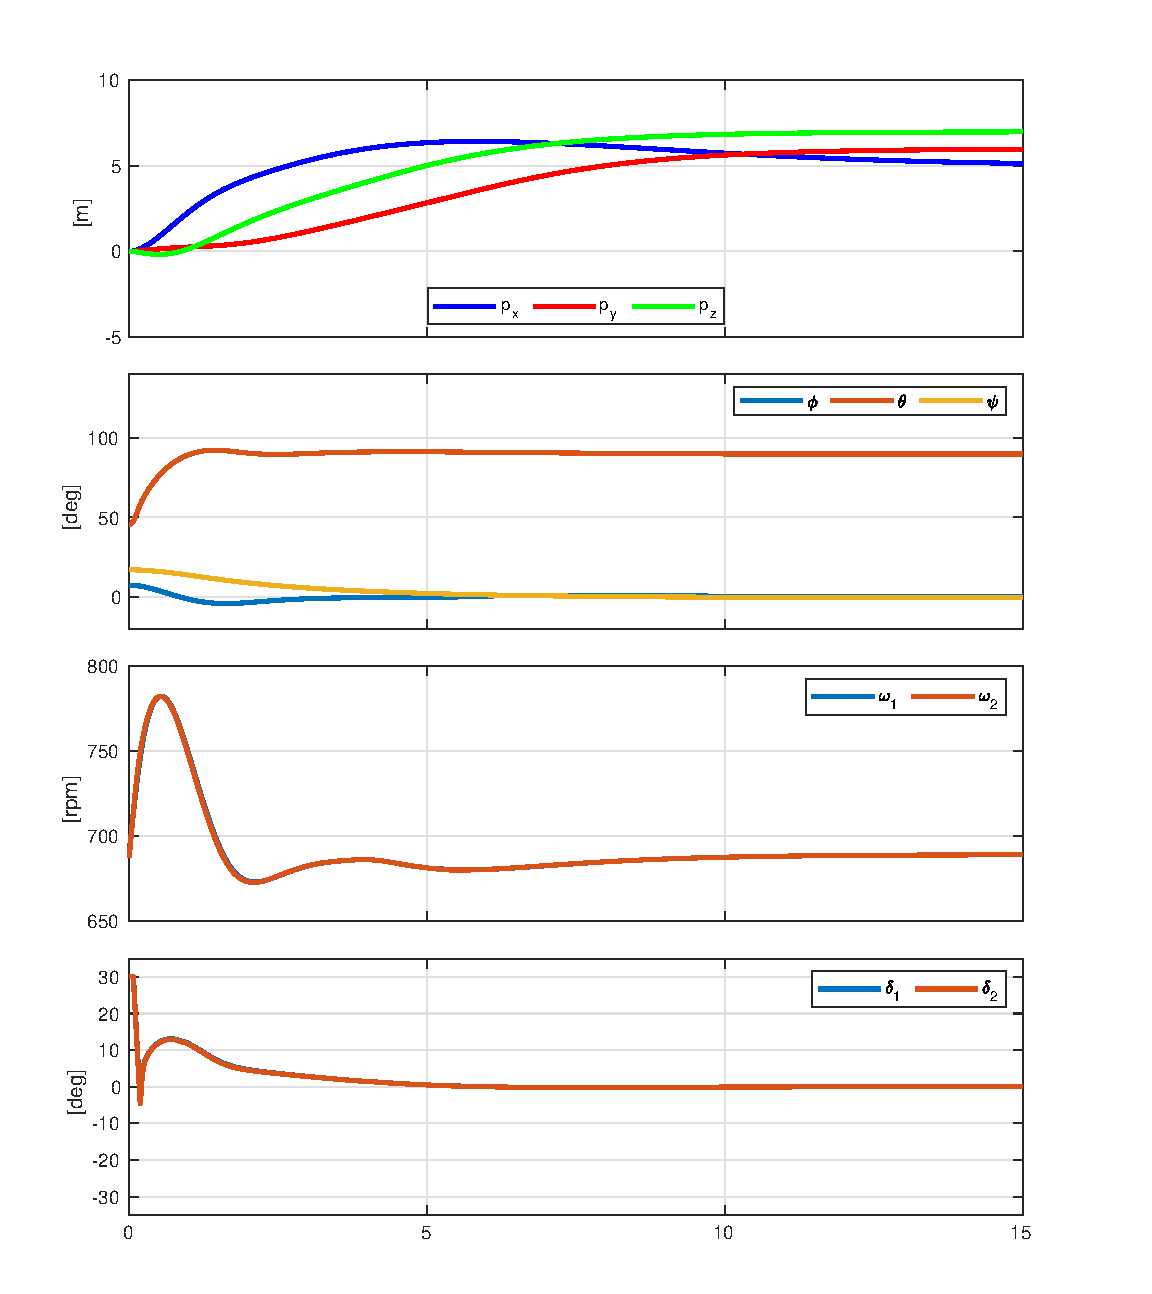
\includegraphics[trim=0cm 0.6cm 0cm 0.6cm,clip,width=0.8\columnwidth]{figures/global2.eps}
    \caption{Simulation de la loi de commande non-linéaire avec la dynamique de DarkO \eqref{eq:dyna_orig}.}
    \label{fig_global_contol}
\end{figure}


\section{Contrôleur par retour d'état linéaire}
Sur la base des observations de la section précédente et étant donné une position cible correspondant à un équilibre $\boldsymbol{p_{\text{eq}}}, \boldsymbol{q_{\text{eq}}}$ tel que caractérisé dans l'équation~\ref{eq:equilibria}, nous concevons ici un contrôleur par retour d'état linéaire capable de produire une réponse plus agressive. Pour cela, nous nous concentrons sur la dynamique linéarisée \eqref{eq:linearized} et proposons une loi de commande de la forme :
\begin{align}
  \boldsymbol{u_{\text{lin}}} := \boldsymbol{u_{\text{eq}}} - \boldsymbol{K} \boldsymbol{\tilde x},
\label{eq:u_lin}
\end{align}
où $\boldsymbol{\tilde x}$ a été introduit dans \eqref{eq:linearized} et $\boldsymbol{K} \in \real^{4 \times 12}$ est un gain de retour d'état qui peut être sélectionné, sur la base des matrices $\boldsymbol{A}_{0}$ et $\boldsymbol{G}_{0}$ apparaissant dans \eqref{eq:linearized}, de telle sorte que la boucle fermée du retour d'état $A_{\text{cl}}:=\boldsymbol{A}_{0}-\boldsymbol{G}_{0}\boldsymbol{K}$ soit exponentiellement stable. 

Dans notre cas, nous avons utilisé une sélection LQR, associée aux matrices de pondération $\boldsymbol{Q} = I_{12}$ et $\boldsymbol{R} = I_{4}$, qui donne une réponse en boucle fermée désirable. La conception LQR fournit également une matrice définie positive  $\boldsymbol{S} \in \real^{12 \times 12}$ (solution de l'équation algébrique de Riccati) garantissant que $\boldsymbol{A}_{\text{cl}}^\top \boldsymbol{S} + \boldsymbol{S} A_{text{cl}} <0$. Il est donc possible d'utiliser $\boldsymbol{S}$ pour former une fonction de Lyapunov.  En particulier, il est bien connu d'après le théorème d'approximation linéaire que la fonction $V(\boldsymbol{\tilde x}) = \boldsymbol{\tilde x}^\top S \boldsymbol{\tilde x}$ est également une fonction de Lyapunov certifiant la stabilité exponentielle locale de $\boldsymbol{x_{\text{eq}}}$ pour la dynamique non-linéaire. Plus précisément, il existe un scalaire positif $\bar v \in \real$ tel que, le long de la dynamique \eqref{eq:dyna_orig}, nous avons :
\begin{align}
\label{eq:Vdecrease}
  V(\boldsymbol{\tilde x}) \leq \bar v \quad \Rightarrow \quad \dot V(\boldsymbol{\tilde x}) := \langle 
\nabla V(\boldsymbol{\tilde x}), \boldsymbol{\dot{\tilde x}}\rangle <0,
\end{align}
pour tout $\boldsymbol{\tilde x} \neq 0$ ; en d'autres termes, le sous-ensemble de $V(\boldsymbol{\tilde x}) \leq \bar v$ est contenu dans le bassin d'attraction de l'équilibre $\boldsymbol{x_{\text{eq}}}$.

La détermination du plus grand scalaire $\bar v$ assurant \eqref{eq:Vdecrease} est un problème complexe et des bornes inférieures conservatrices peuvent être déterminées en quantifiant l'effet des non-linéarités sur la dynamique. Puisque $\boldsymbol{\dot{\tilde x}}$ est une fonction de $\boldsymbol{x}$, il est assez facile d'évaluer algébriquement $\dot V(\boldsymbol{\tilde x})$ pour un grand nombre d'extractions aléatoires de la variable $\boldsymbol{\tilde x}$, afin d'obtenir une estimation probabiliste du plus grand scalaire $\bar v$. Des garanties rigoureuses sur ces sélections peuvent être obtenues en appliquant les résultats de \cite{tempo2013randomized}, mais une évaluation de 10000 échantillons a confirmé que la valeur $\bar v = 400$ est une bonne sélection satisfaisant \eqref{eq:Vdecrease}.


\begin{figure}[ht!]
    \centering
    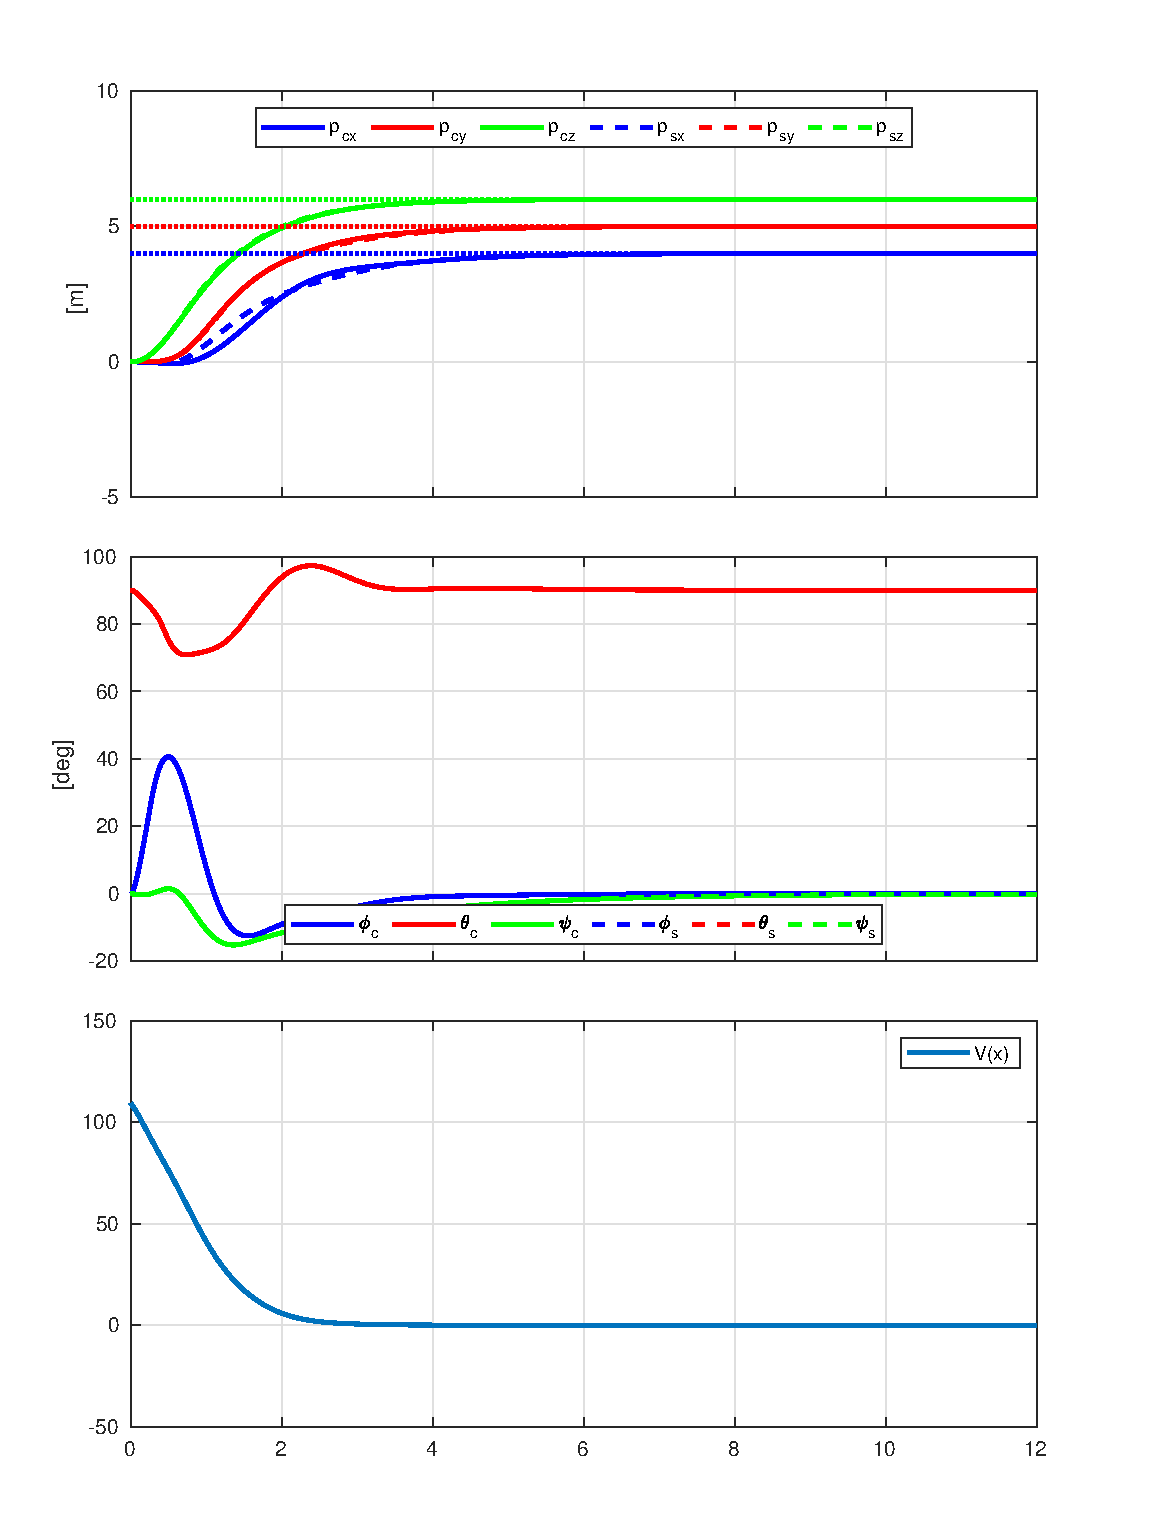
\includegraphics[trim=0cm 0.6cm 0cm 1cm,clip,width=0.8\columnwidth]{figures/converge2.eps}
    \caption{Simulation du modèle complet \eqref{eq:dyna_orig} (continue) et simplifié \eqref{eq:withouwind} (pointillé) avec $\boldsymbol{u} = \boldsymbol{u}_{\text{lin}}$ défini dans 
    \eqref{eq:u_lin} et comme une condition initiale $\tilde{ \boldsymbol{x}}_0$ dans le bassin d'attraction.}
    \label{fig_linearize_conv}
\end{figure}

La figure \ref{fig_linearize_conv} montre une simulation commençant à l'origine avec un drone vertical et des vitesses linéaires et angulaires initiales sont nulles. La position cible est $\boldsymbol{p_{\text{eq}}} = [4,~5,~6]$ avec une stabilisation en vol stationnaire (drone vertical) avec $\beta = 0$. La ligne pointillée représente la position de la cible sur chaque axe. Le dernier graphique montre la décroissance exponentielle souhaitable de $V$
La figure \ref{fig_linearize_conv} montre à la fois la simulation du modèle complet (continue) \eqref{eq:dyna_orig} et du modèle non linéaire simplifié \eqref{eq:withouwind} (en pointillé), ce qui montre des différences dans la phase transitoire.
Lorsqu'on fournit une position cible plus importante $\boldsymbol{p_{\text{eq}}} =[8,~9,~10]$(avec la même orientation), la condition initiale se situe en dehors du bassin d'attraction et une divergence apparait, comme le montre la figure~\ref{fig_linearize_div}.

\begin{figure}[ht!]
    \centering
    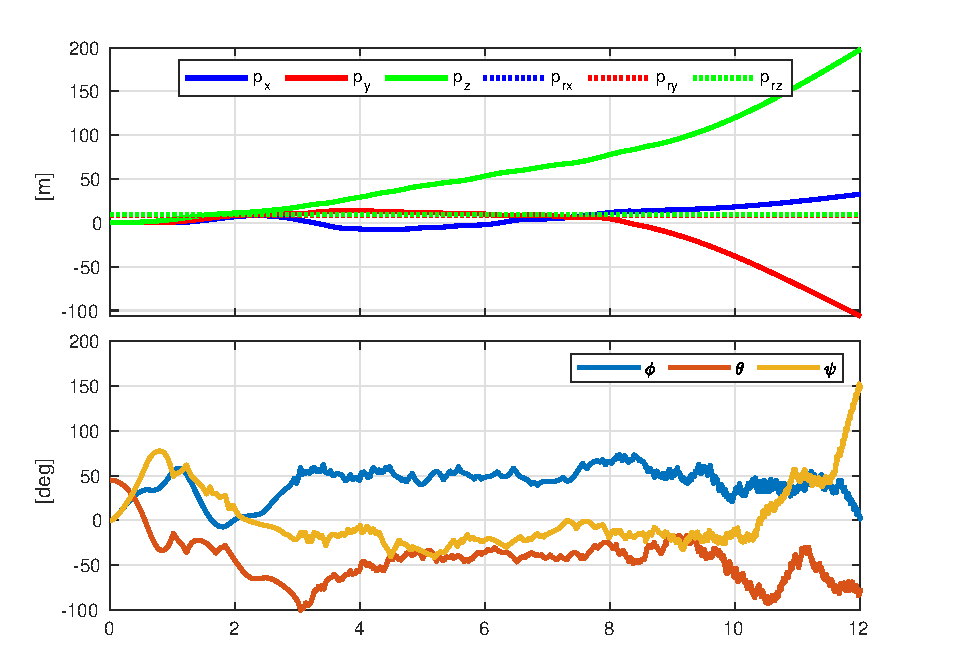
\includegraphics[trim=0cm 0cm 0cm 0cm,clip,width=0.8\columnwidth]{figures/diverge2.eps}
    \caption{Simulation divergente du modèle complet \eqref{eq:dyna_orig} avec $\boldsymbol{u} = \boldsymbol{u}_{\text{lin}}$ défini dans 
    \eqref{eq:u_lin} et une condition initiale $\tilde{ \boldsymbol{x}}_0$ en dehors du bassin d'attraction.}
    \label{fig_linearize_div}
\end{figure}



\section{Conception d'une commande locale-globale basée sur l'hystérésis}
\label{sec:ctrl_hyste}
 
Inspirés par les stratégies locales-globales présentées dans \cite[Ex. 1. 7]{65}, similaire à la solution présentée dans \cite{AndreettoFZ16}, nous utilisons un mécanisme hybride pour basculer entre le contrôleur local agressif \eqref{eq:u_lin} (tant que l'état se trouve dans le bassin d'attraction de l'équilibre) et le contrôleur non linéaire moins agressif \eqref{eq:u_nonlin}, qui fournit une plus grande région d'attraction (et peut être appelé, par abus de langage, le « contrôleur global »). À cette fin, nous ajoutons à l'état du contrôleur une variable d'état logique $\ell \in \{0,1\}$, qui régit le choix de l'entrée de contrôle entre \eqref{eq:u_nonlin} et \eqref{eq:u_lin} tel que
\begin{align}
\label{eq:u_hybrid}
  \boldsymbol{u}=\boldsymbol{u}_{\text{hyb}} := \ell \boldsymbol{u}_{\text{nl}} + (1-\ell) \boldsymbol{u}_{\text{lin}},
\end{align}
Nous nous assurons, grâce à la dynamique hybride, que $\ell$ ne peut prendre que des valeurs dans $\{0,1\}$. Sa dynamique est définie par : 
\begin{align*}
    \left\{
        \begin{array}{ll}
            \dot \ell = 0,& \chi \in \mathcal{C}\\
            \ell^{+} = 1-\ell,& \chi \in \mathcal{D}
        \end{array}
    \right.
\end{align*}
où $\chi = \left[\boldsymbol{p},~ \boldsymbol{v},~ \boldsymbol{q},~  \boldsymbol{\omega},~ l\right]$ est l'état complet de la boucle fermée et $\mathcal{C}$ et $\mathcal{D}$ sont, respectivement, les ensembles continus et discret, définis par
\begin{align*}
    & \mathcal{C} := \mathcal{C}_{0} \cup \mathcal{C}_{1}, ~ \mathcal{D} := \mathcal{D}_{0} \cup \mathcal{D}_{1},\\
   & \mathcal{C}_{0} :=\{\boldsymbol{\chi} \in \mathbb{R}^{14}:~ V(\boldsymbol{\tilde x}) \le \overline{v} \mbox{ and } \ell=0\}\\
   & \mathcal{C}_{1} :=\left\{\boldsymbol{\chi} \in \mathbb{R}^{14}:~ V(\boldsymbol{\tilde x}) \ge \underline{v} \mbox{ and } \ell=1 \right\}\\
   & \mathcal{D}_{0} :=\left\{\boldsymbol{\chi} \in \mathbb{R}^{14}:~ V(\boldsymbol{\tilde x}) \geq \overline{v}\mbox{ and } \ell=0 \right\}\\
   & \mathcal{D}_{1} :=\left\{\boldsymbol{\chi} \in \mathbb{R}^{14}:~ V(\boldsymbol{\tilde x}) \leq \underline{v}\mbox{ and } \ell=1 \right\}
\end{align*}
où $V(\boldsymbol{\tilde x}) := \boldsymbol{\tilde x}^\top S \boldsymbol{\tilde x}$  a été défini dans la section précédente, $\overline{v}=400$ a été déterminé pour satisfaire \eqref{eq:Vdecrease} et $\underline{v}$ est toute constante positive satisfaisant $\underline{v}<\overline{v}$ (un choix plus grand de $\underline{v}$ augmente la marge d'hystérésis, mais retarde le changement de loi de commande). Dans notre cas, nous choisissons $\underline{v}= 350$.

Le résultat suivant est une conséquence immédiate des résultats de \cite[Ex. 1.7]{65} et des propriétés de nos modèles linéaires et non linéaires.

\begin{proposition}
    Avec l'action du bouclage hybride \eqref{eq:u_hybrid}, la boucle fermée présente le même bassin d'attraction que celui associé au contrôleur non linéaire \eqref{eq:u_nonlin}, quand elle utilise le contrôleur linéaire \eqref{eq:u_lin}.
\end{proposition}

Nous avons réalisé plusieurs simulations de la boucle fermée à l'aide de la \textit{toolbox} Matlab \cite{sanfelice_2017}. Les simulations sont effectuées avec le modèle complet du drone \eqref{eq:dyna_orig}, comprenant tous les effets aérodynamiques non linéaires. Un exemple de simulation est présenté dans la Figure~\ref{fig_sim}, où nous initialisons le drone à l'origine avec une orientation nulle sauf pour l'angle de tangage fixé à 45 degrés. L'orientation de la cible est en configuration de vol stationnaire vertical et la position de la cible est assignée à $\boldsymbol{p_{\text{eq}}} = [50,~25,~12.5]$.

\begin{figure}[!ht]
    \centering
    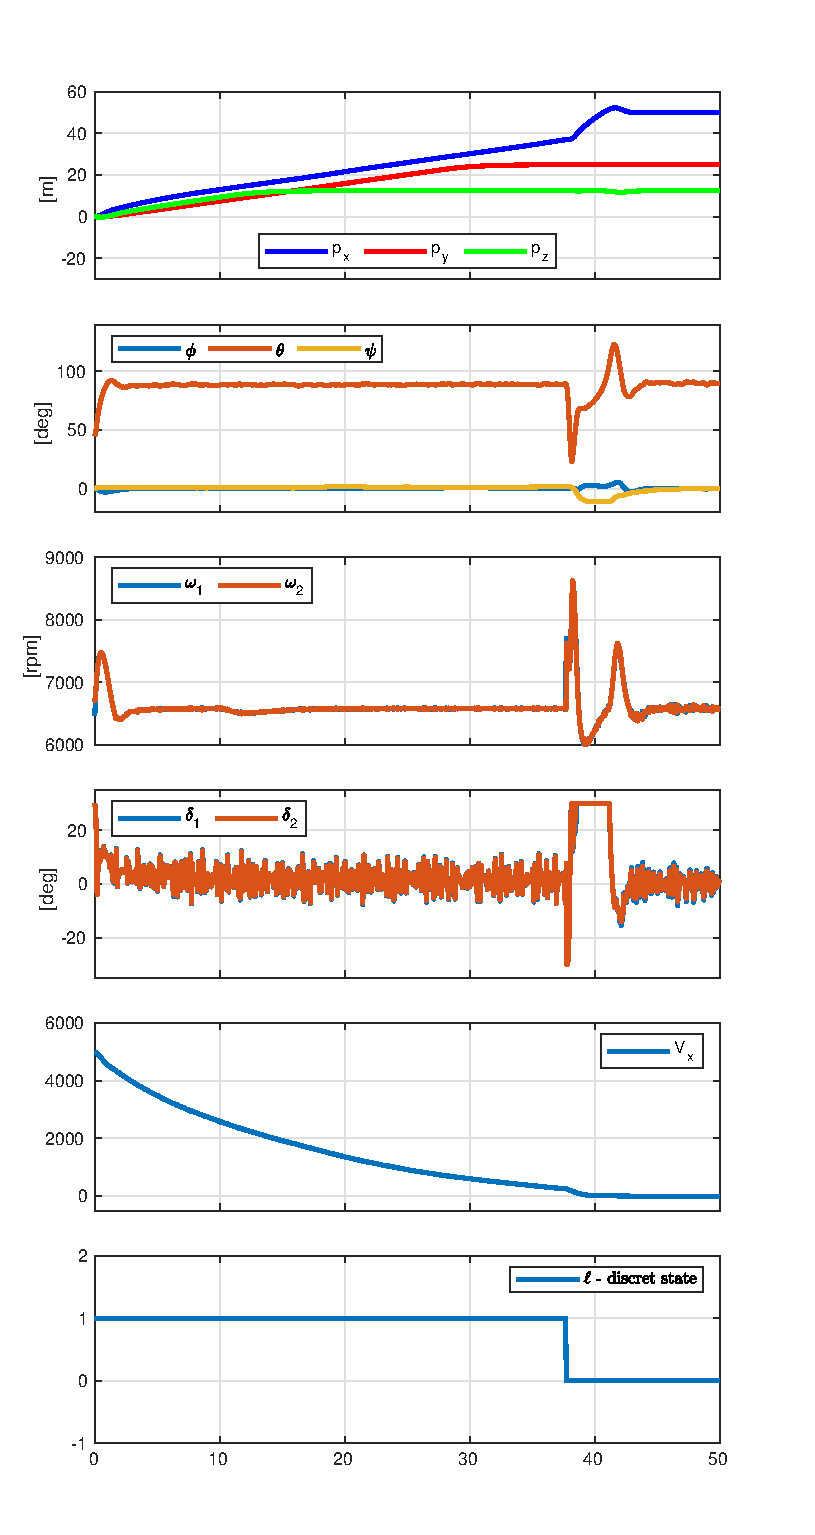
\includegraphics[trim=0cm 0cm 0cm 1.1cm,clip,width=0.8\columnwidth]{figures/switch_paper2.eps}
    \caption{Simulation en boucle fermée avec le contrôleur hybride \eqref{eq:u_hybrid}.}
    \label{fig_sim}
\end{figure}

Nous observons que sur la période $t \ dans \left[0,38\right]$, le drone
présente une convergence élégante, mais lente vers la position cible souhaitée en utilisant le contrôleur global ($\ell=1$). À ce moment-là, l'état discret $\ell$ entre dans l'ensemble $\mathcal{D}_1$ et le contrôleur local plus agressif est activé jusqu'à la convergence vers l'équilibre souhaité.

Pour obtenir des simulations réalistes, les mesures sont affectées par 
le bruit des capteurs. La robustesse intrinsèque de la rétroaction hybride, établie dans le [Chapitre 7]{65}, est confirmée par le maintient des performances malgré le bruit de mesure.

\section{Conclusion du Chapitre \ref{chap:hybrid}}






\chapter{Commande robuste longitudinale d'une maquette}
\minitoc
\label{chap:3DOF}

\section{Motivation}
\label{sec:motivation3DOF}
Les simulations en boucle fermée avec le contrôleur \eqref{eq:u_hybrid} développé dans la section \ref{sec:ctrl_hyste} montrent qu'en présence d'un vent horizontal constant dans le plan $(x_{[b]},z_{[b]})$, le drone modifie son angle de tangage. Ce comportement a également été observé lors d'essais en soufflerie avec le dispositif expérimental \cite{olszaneckibarthHal-02542982}. Intuitivement, une réduction de l'angle d'attaque entraîne une diminution de la surface exposée au vent, de manière à réduire la force de traînée, ce qui a une forte incidence sur la position. Dans le même temps, le flux d'air dû au vent constant génère une portance, compensée par une réduction de la poussée de l'hélice et une réduction conséquente de la consommation du drone. L'objectif de la maquette décrite ici est d'évaluer expérimentalement l'effet du vent sur le dispositif DarkO.

De plus, il faut noter que le changement de l'angle d'attaque du drone a un impact sur la mesure du vent. Comme la sonde de Pitot est fixée sur le corps du drone, cette dernière se trouve être en rotation lors de la transition. On comprend donc que la mesure du vent ne sera valide qu'en vol d'avancement, à haute vitesse. En vol stationnaire ou lors de la transition, nous n'avons pas de mesure du vent, ni des rafales impactant le drone.

Nous allons donc proposer dans ce chapitre une méthode de commande linéaire n'utilisant pas de mesure de vent pour stabiliser le drone dans une position de l'espace. Toutefois, nous commencerons par une stabilisation longitudinale sur une dynamique à trois degrés de liberté pour tester notre loi de commande. Cette loi de commande est locale et n'est valide que dans un environnement proche du point d'équilibre. Ce bouclage pourrait être utilisé en remplacement de la loi LQR proposée dans la section \ref{sec:ctrlLin}.

\section{Présentation de la maquette expérimentale}
\label{sec:test_bench}



\subsection{Description physique, capteurs et actionnements}
Le prototype développé comprend des pièces imprimées en 3D, en Onyx et PLA  \nomenclature[]{\(PLA\)}{Thermoplastique : acide polylactique} (acide polylactique, un polyester thermoplastique). Le drone est spécialement conçu pour réaliser des expériences devant une soufflerie, avec un comportement semblable à celui de DarkO en raison de leur forme similaire (voir Figure \ref{fig:real_test_bench}). La partie centrale, qui contient l'avionique embarquée (pilote automatique, GPS, etc.) dans DarkO, a été remplacée ici par un joint tournant à un degré de liberté (voir Figure \ref{fig:rotation}). Les ailes sont les mêmes que celles du DarkO, avec les contrôleurs électroniques de vitesse (ESC), régissant la vitesse du moteur \textit{brushless}, placés dans les ailes.

Comme décrit dans la section \ref{sec:motivation3DOF}, nous souhaitons représenter et étudier le degré de liberté de l'axe $y_{\text{b}}$ du drone DarkO. Le tube principal en carbone reliant les deux ailes est utilisé comme axe de rotation. Ce tube est fixé sur deux roulements espacés de \SI{28.5}{\milli\meter} afin d'obtenir une fixation solide de l'ensemble. Cet axe de rotation est équipé d'un codeur optique rotatif en quadrature pour mesurer précisément l'orientation de l'appareil. L'avantage de ce capteur est qu'il ne produit pas de couple résistant sur l'axe de rotation. Ce codeur offre 4000 impulsions par tour, ce qui donne une résolution de $\SI{0.09}{\degree}/impulsion$.
\begin{figure}[!ht]
    \centering
    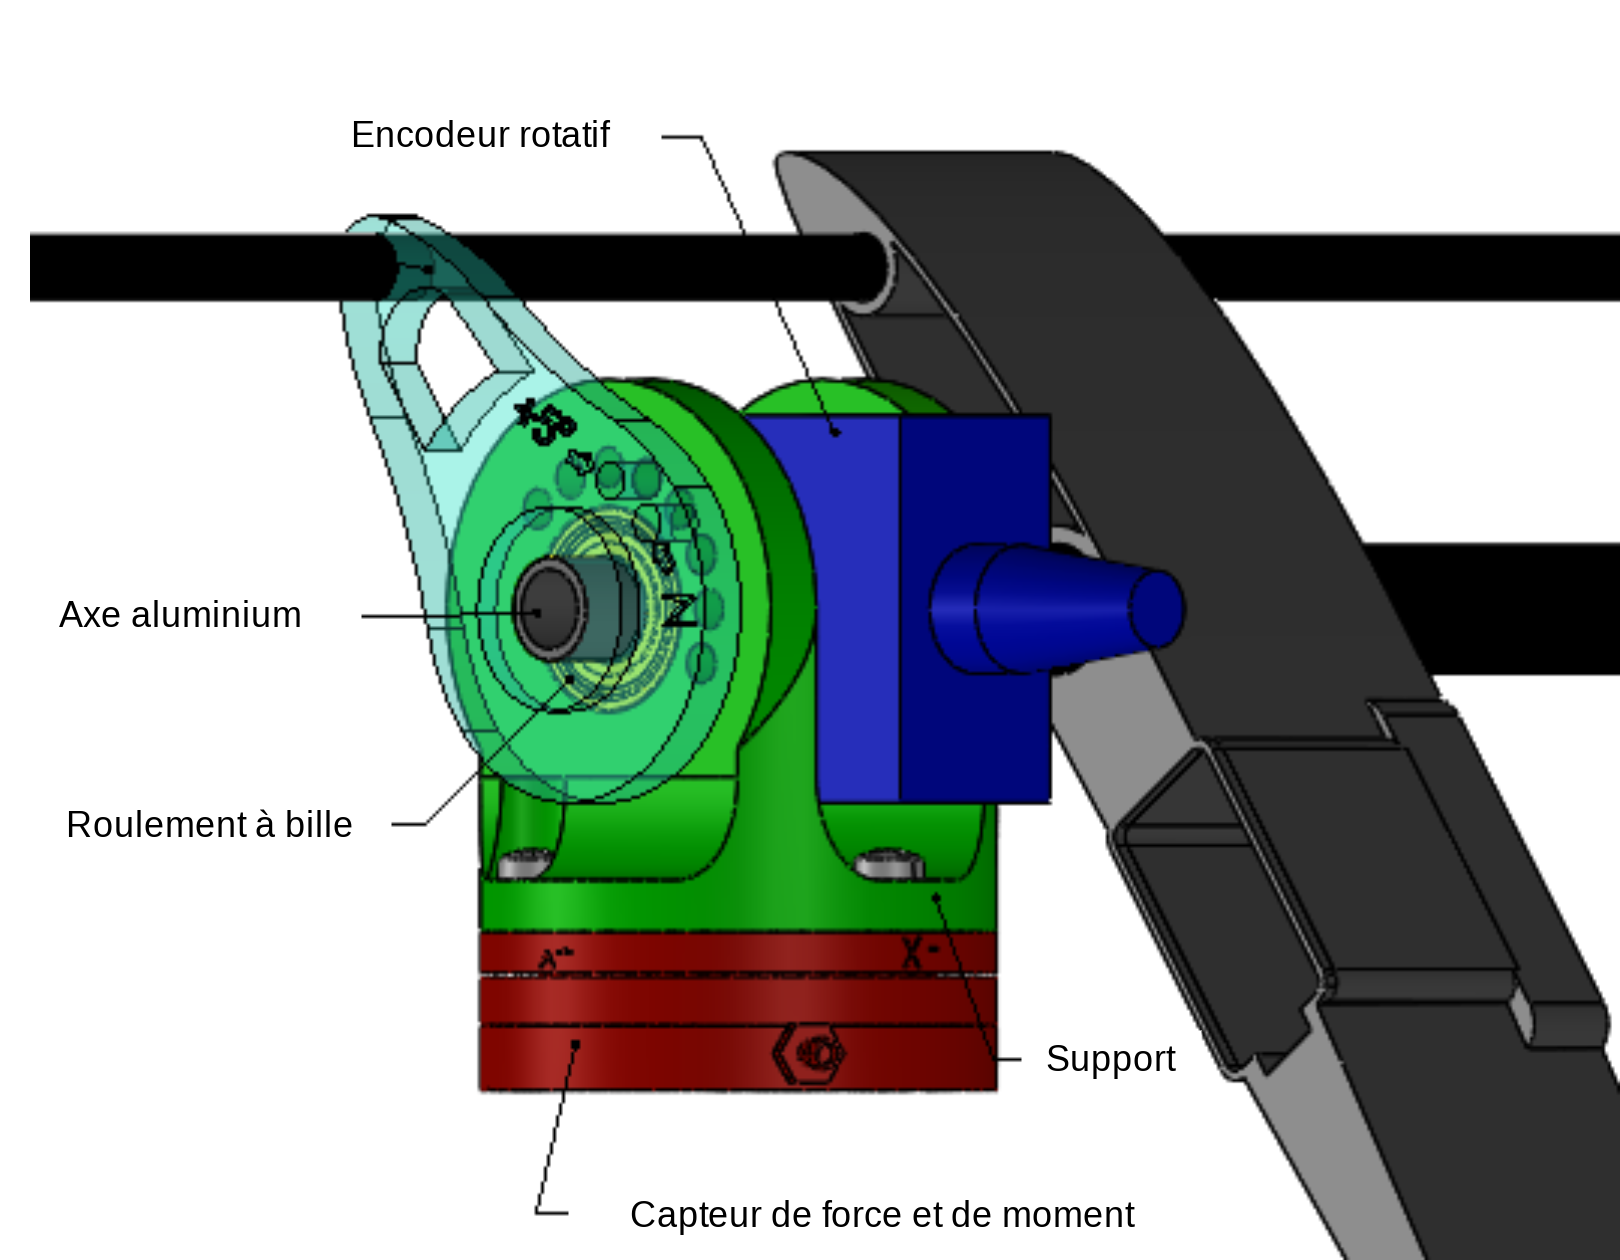
\includegraphics[width=0.6\columnwidth]{figures/MontageSupport2.png}.
    \caption{Montage à un degré de liberté.}
    \label{fig:rotation}
\end{figure} 

Comme le montre la Figure \ref{fig:rotation}, l'indexeur et le support sont percés pour que la rotation puisse être bloquée, par une vis, à des positions connues ($0^\circ$, $90^\circ$, etc.). Le verrouillage de l'appareil permet une initialisation correcte de l'encodeur incrémental. Le verrouillage permet également de placer l'appareil dans des positions exactes spécifiques afin d'identifier les coefficients aérodynamiques. 

Le mécanisme est également équipé d'un capteur de forces et de moments à 6 degrés de liberté (DOF), qui permet de mesurer la force exercée sur le dispositif expérimental par le support. Le banc d'essai expérimental est également équipé d'un fil chaud pour mesurer la vitesse de l'air affectant la maquette. 

\begin{figure}[!ht]
    \centering
    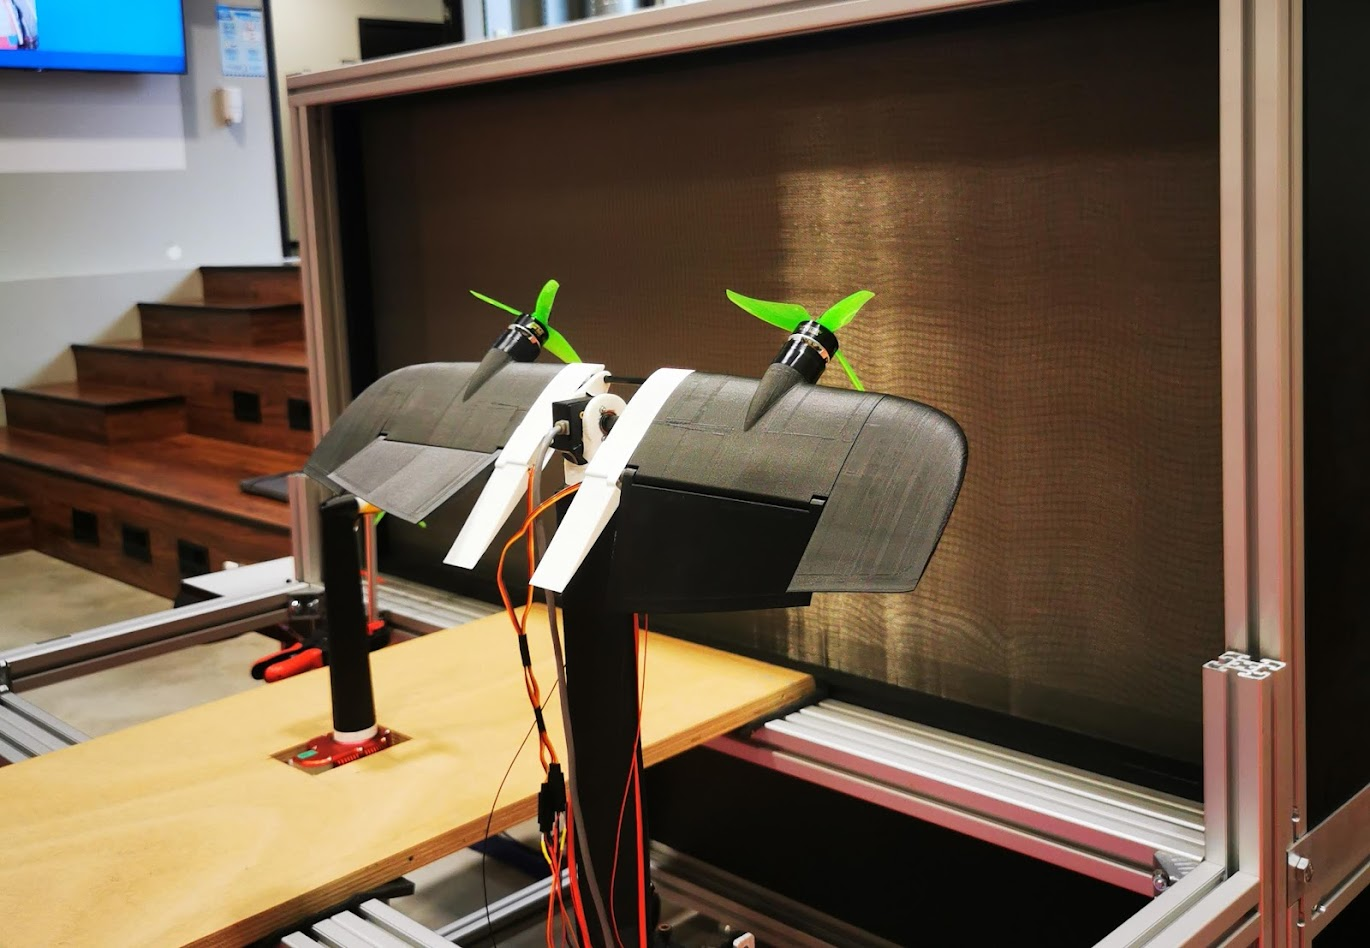
\includegraphics[trim=0cm 5cm 0cm 6cm,clip,width=0.8\columnwidth]{figures/real_test_bench-min.jpg}
    \caption{Modèle de DarkO à un seul degré de liberté devant le \textit{WindShape}.}
    \label{fig:real_test_bench}
\end{figure}
La photo de la Figure \ref{fig:real_test_bench} montre le dispositif expérimental dans son environnement de test. Le drone est placé devant une soufflerie ouverte, appelée \textit{WindShape}, qui génère un vent horizontal compris entre 2 et 16 \SI{}{\meter\per\second}. Ainsi, lors de nos tests, nous considérons que la composante verticale du vent est nulle. Le drone est placé au centre du \textit{WindShape}, dans la zone d'écoulement la plus laminaire, tandis que le capteur à fil chaud est placé aussi près que possible du drone. 

La géométrie du dispositif expérimental permet de placer les câbles d'alimentation et de signal près du centre de rotation afin de minimiser leurs effets de friction sur la structure. Malgré cela, le système de rotation interfère inévitablement avec le drone, en créant des forces parasites, notamment de la traînée. La surface projetée de l'articulation étant faible par rapport à la surface de l'aile, la traînée générée par ce support est faible par rapport à la traînée de l'aile et des hélices, et peut donc être négligée. Un diagramme schématique des composants du dispositif expérimental et de leurs interconnexions est présenté à la Figure \ref{fig:archi}.

\begin{figure}[!ht]
    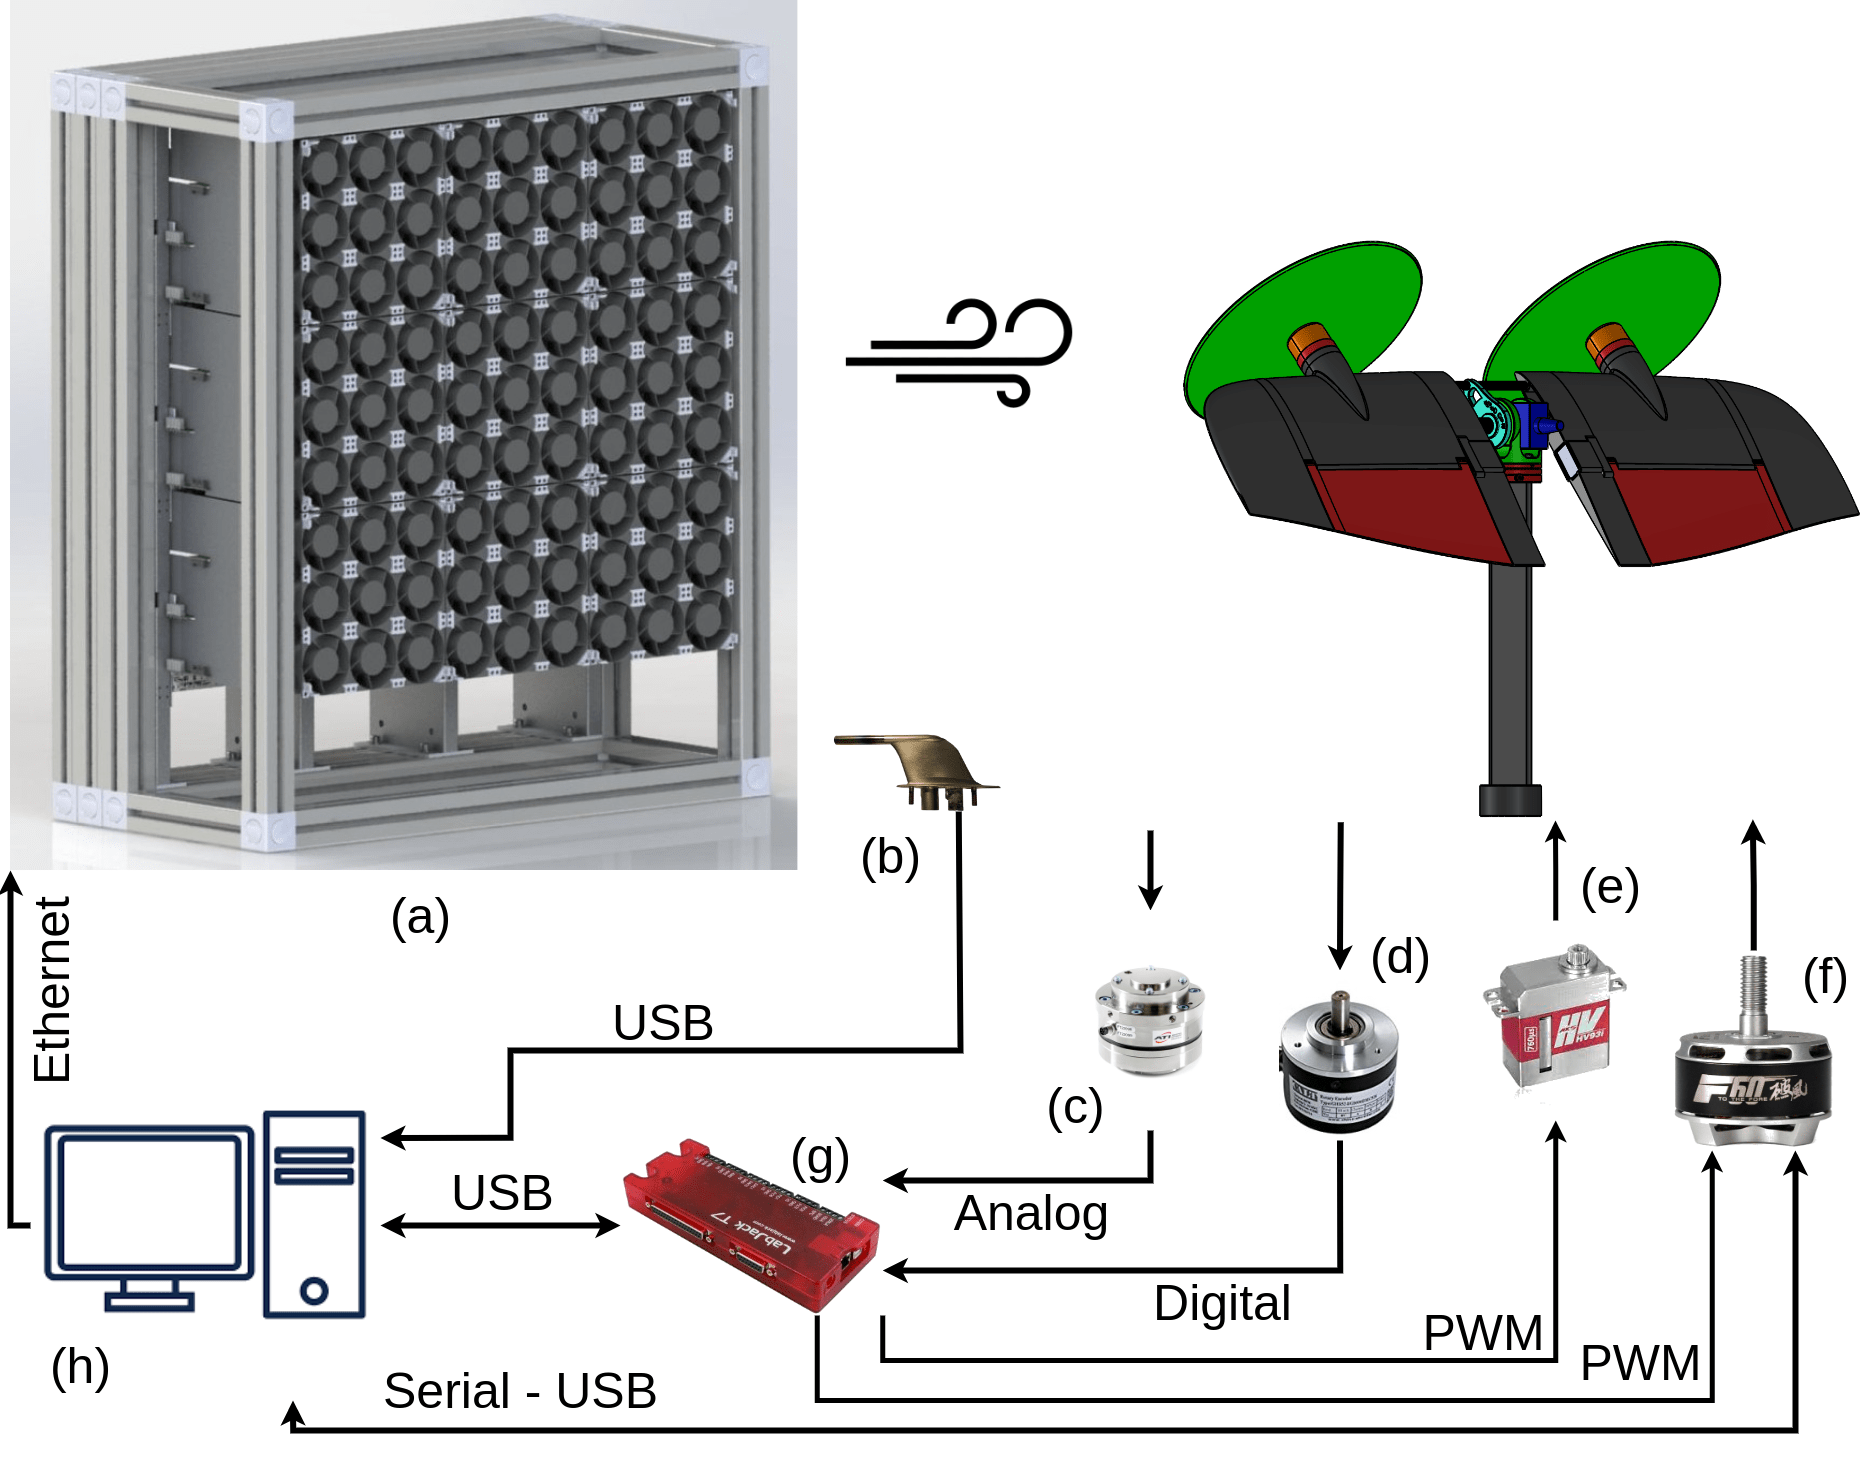
\includegraphics[width=\columnwidth]{figures/maquette-min.png}
    \caption{Architecture d'essai en vol virtuel : \textit{WindShape} (a) ; capteur de vitesse (b) ; capteur de forces et moments (c) ; encodeur rotatif (d) ; servomoteur (e) ; moteur \textit{brushless} + ESC (f) ; LabJack (g) ; ordinateur de contrôle (h)}
    \label{fig:archi}
\end{figure}

Les moteurs (f) sont alimentés par une batterie externe de 12v 20Ah et les servomoteurs (e) sont alimentés par du 5 V, via un module d'acquisition LabJack T7 \cite[]{LabJack} (g). Le module LabJack (g) concentre la plupart des signaux des capteurs et des actionneurs : six entrées analogiques pour le capteur de force/couple (c), deux entrées numériques en quadrature pour l'encodeur rotatif (d), une entrée analogique (ou une liaison série selon le capteur) pour le capteur de vitesse (b), deux sorties numériques PWM (Pulse Width Modulation) pour les moteurs (f) et deux sorties numériques PWM pour les servomoteurs (e). 

Les élevons sont commandés par des servomoteurs qui ne fournissent pas de signal de mesure de la position. Nous utilisons donc le point de consigne, en supposant que les actionneurs soient parfaits. Cela est raisonnable en raison de la saturation logicielle imposée à l'entrée des élevons et du dimensionnement correct des servomoteurs par rapport aux forces impliquées. 
Le LabJack (g) possède une interface de programmation d'application (API), permettant une connexion avec un ordinateur. Nous avons développé un code Python qui communique avec le LabJack afin de récupérer les valeurs des capteurs, de calculer la commande à appliquer aux servomoteurs selon le schéma de contrôle présenté ci-dessous et de générer les signaux de sortie pour les servomoteurs. Les données collectées par le LabJack sont enregistrées afin d'être utilisées pour le post-traitement et de générer le graphique présenté dans la section \ref{sec:exp3DOF}. 

\nomenclature[]{\(PWM\)}{Modulation de largeur d'impulsions (\textit{Pulse Width Modulation})}
\nomenclature[]{\(API\)}{Interface de programmation d'application (\textit{Application Programming Interface})}

Le \textit{WindShape} dispose également d'une API lui permettant d'être contrôlé via un réseau Ethernet. Le code Python développé peut assigner la vitesse du vent générée par le \textit{WindShape} et donc agir sur le modèle. Il est ainsi possible de tester un ensemble de configurations de vols stationnaires et les transitoires associés dans la même campagne d'essais, sans aucune action sur le modèle. 


\subsection{Simulation des mouvements du drone}
Le prototype étant relié à un support fixe, il n'est pas possible de reproduire expérimentalement le mouvement de translation.  Nous avons donc inclus une simulation logicielle du mouvement en intégrant les mesures de force disponibles au niveau de la fixation. La vitesse de translation (respectivement la position) du drone est obtenue par intégration simple (respectivement double) des données mesurées par le capteur de force. Par souci de simplicité, nous négligeons l'influence aérodynamique de la vitesse (simulée) sur l'aile. En particulier, à partir des équations \eqref{eq:dyna_orig_a} et \eqref{eq:dyna_orig_b}, nous obtenons le modèle simplifié suivant : 
\begin{subequations}\label{eq:accel_sensor}
    \begin{align}
        \boldsymbol{\dot v} &= \boldsymbol{g} + \frac{1}{m}\left( R(\boldsymbol{q})(F\boldsymbol{u} +  D_{\text{f}}(\delta) R^\top(\boldsymbol{q})\lVert \boldsymbol{w} \rVert \boldsymbol{w}) \right)\\
        &= \boldsymbol{g} + \frac{1}{m} \boldsymbol{F}_{meas} \label{eq:sub_accel_sensor},
    \end{align}
\end{subequations}
où $\boldsymbol{F}_{meas}$ représente les forces mesurées par le capteur dans le repère inertiel corrigé du biais. Pour calibrer la correction du biais, lors de l'initialisation, les forces mesurées sont moyennées sur 6000 échantillons, le modèle étant bloqué dans une position stable (angle de tangage à 0°, c'est-à-dire orientation verticale). Pour éliminer le biais de la force mesurée à chaque mesure, nous soustrayons l'effet de la gravité sur le modèle de la mesure. Une masse artificielle $m$ est attribuée à la dynamique du logiciel dans la boucle conformément à \eqref{eq:sub_accel_sensor}, ce qui permet de tester plusieurs configurations afin de mieux apprécier l'influence de la masse du drone sur d'éventuels événements transitoires de saturation. Cela permet d'étudier des scénarios impliquant la masse non négligeable de la batterie, qui n'est pas présente dans notre modèle. Bien que cette manipulation soit aisée, elle ne représente pas parfaitement la réalité car nous ne tenons pas compte de la répartition des masses dans le drone et donc des modifications de l'inertie.
La vitesse et la position transitoire du drone sont ensuite obtenues par intégration numérique simple et double de l'accélération comme dans \eqref{eq:accel_sensor}, en utilisant une intégration numérique trapézoïdale.

\section{Contrôle linéaire, architecture PI sur maquette à 3 DOF}
\label{sec:3dofcmd}
Dans la section \ref{sec:ctrl_hyste}, nous avons proposé un bouclage proportionnel stabilisant une position de vol stationnaire en l'absence de vent (sans perturbation). Nous proposons ici une extension incluant une action intégrale, adaptée au fonctionnement avec une perturbation non mesurée représentée par un vent constant. L'objectif est de stabiliser le drone à la position de référence, en rejetant une perturbation de vent constant inconnue.
Les matrices de gain associées au gain intégral et proportionnel seront optimisées suivant un schéma de synthèse $H_{\infty}$ combinant à la fois des critères de robustesse et de performance. Nous mettons donc en œuvre une synthèse robuste basés sur des critères $H_{\infty}$ sous contrainte d'une structure PI multidimensionnelle (MIMO).

\subsection{Description du schéma de contrôle}
Nous expérimentons la situation avec le vent agissant uniquement le long de l'axe $x_{i}$, avec le drone orienté vers le vent, c'est-à-dire avec des angles de roulis et de lacet nuls. Dans cette configuration, le vent n'agit que sur la vitesse linéaire le long des axes $x_{b}$ et $z_{b}$, et ne génère qu'un moment autour de l'axe $y_{b}$. Un examen attentif de la commande et des matrices d'entrée des perturbations $\boldsymbol{F}$, $\boldsymbol{M}$ dans \eqref{eq:FandM} suggère une architecture de commande efficace pour rejeter une perturbation constante. En effet, les élevons et les hélices peuvent être utilisés symétriquement pour générer respectivement un moment autour de l'axe $y_{b}$ et une force le long de l'axe $x_{b}$, compensant ainsi l'effet de la perturbation. Néanmoins, il reste une force le long de l'axe $z_{b}$ à compenser et une action intégrale peut converger asymptotiquement vers la force désirée, même avec une perturbation du vent non mesurée $\boldsymbol{w}$. Nous pouvons ainsi stabiliser le drone à une position de vol stationnaire, différente de l'équilibre sans vent. La solution de contrôle exploite le degré de liberté de l'angle de tangage pour compenser l'effet du vent.

\begin{figure}[ht!]
    \centering
    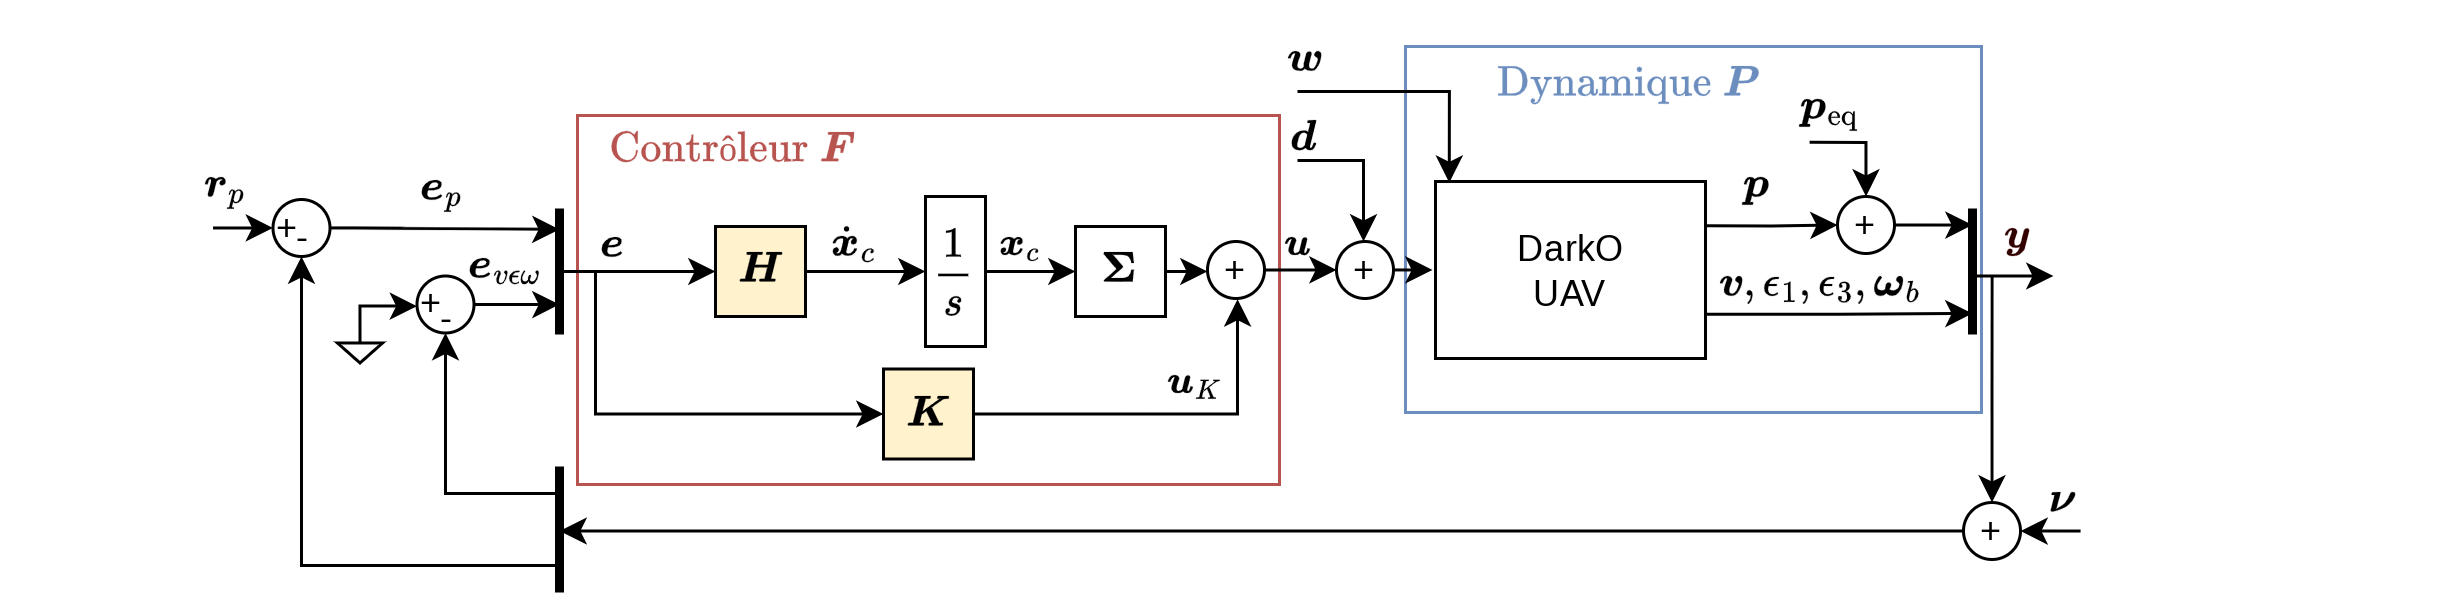
\includegraphics[trim=5cm 0cm 0cm 0cm,clip,width=1\columnwidth]{figures/commande_integrale_3DOF.png}
    \caption{Schéma de commande linéaire, proportionnel-intégral.}
    \label{fig:commande_int3DOF}
\end{figure}
Le contrôleur proposé, représenté sur la Figure \ref{fig:commande_int3DOF}, correspond à :

\begin{subequations}
    \label{eq:ctrl3dof}
    \begin{align}
        \boldsymbol{e}_{p} &= \boldsymbol{r}_{p} - \boldsymbol{p},\\
        \boldsymbol{e} &= \smallmat{
        \boldsymbol{e}_{p}^\top & \boldsymbol{e}_{v\epsilon\omega}^\top}^\top, \quad \dot{\boldsymbol{x}}_{c} = \boldsymbol{H} \boldsymbol{e}, \quad    \boldsymbol{u} = \boldsymbol{\Sigma} \boldsymbol{x}_{c} + \boldsymbol{u}_{K},
        \\
        \boldsymbol{\Sigma} &:= \begin{bmatrix} \! 1 \!&\! 1\! & \!0\! &\! 0\!\\ \!0\! & \!0\! & \!1 \!& \!1\!\end{bmatrix}^\top, \quad
        \boldsymbol{u}_{K} = \boldsymbol{K} \boldsymbol{e} ,
    \end{align}
\end{subequations}

% \begin{subequations}
%     \begin{align}
%         \label{eq:ctrl3dof}
%         \dot{\boldsymbol{x}_{c}} = \boldsymbol{H}(\boldsymbol{y}-\begin{bmatrix}\boldsymbol{r}_{p}\\\mathbb{0}_{8\times 1} \end{bmatrix}), \quad
%         \boldsymbol{y} = \boldsymbol{S} \boldsymbol{x},\quad
%         \boldsymbol{u} = \Sigma \boldsymbol{x}_{c} + \boldsymbol{K}(\boldsymbol{y}-\begin{bmatrix}\boldsymbol{r}_{p}\\\mathbb{0}_{8\times 1} \end{bmatrix}),\\
%         \boldsymbol{S} =\begin{bmatrix} \mathbb{I}_{7} &  \mathbb{0}_{7\times 5} \\
%          \mathbb{0}_{4\times 8} &  \mathbb{I}_{4}
%           \end{bmatrix}, \quad
%           \boldsymbol{\Sigma} = \begin{bmatrix} 1 & 1 & 0 & 0\\ 0 & 0 & 1 & 1\end{bmatrix}^\top,
%     \end{align}
% \end{subequations}

où $\boldsymbol{x}_{c} \in \mathbb{R}^{2}$ est l'état de l'intégrateur ; $\boldsymbol{r}_{p} \in \mathbb{R}^{3}$ est la référence constante comprenant une position cible pour le mouvement de translation ; $\boldsymbol{\Sigma}$ est une matrice d'allocation d'entrée qui permet d'affecter la première composante de l'état de l'intégrateur à la commande du moteur et la seconde composante à la commande de la gouverne de profondeur. $\boldsymbol{K}$, $\boldsymbol{H}$ sont des gains constants à sélectionner pour que la matrice linéaire de la boucle fermée $\boldsymbol{A}_{cl}$ caractérisant la boucle fermée linéaire soit Hurwitz, afin d'assurer la stabilisation avec la dynamique linéarisée liée au scénario sans vent \eqref{eq:withouwind}.

De manière synthétique, la matrice \eqref{eq:close_matrix} décrit la boucle fermée illustrée à la Figure~\ref{fig:commande_int3DOF} avec \eqref{eq:ctrl3dof} : un retour de sortie avec 11 sorties, comprenant les trois positions, les trois vitesses linéaires, deux des trois angles ($\epsilon_{1}$ et $\epsilon_{3}$) et les trois vitesses angulaires.
\begin{align} \label{eq:close_matrix}
    \begin{gathered}
        \boldsymbol{A}_{cl} \!= \!
        \begin{bmatrix}\boldsymbol{A} & \mathbb{0}_{12\times 2} \\ \boldsymbol{H} & \mathbb{0}_{2\times 2}\end{bmatrix} \!- \!\begin{bmatrix}\boldsymbol{G} \\ \mathbb{0}_{2\times 4}\end{bmatrix} \left( \boldsymbol{K} -  \begin{bmatrix}\mathbb{0}_{4\times 12} & \boldsymbol{\Sigma} \end{bmatrix}\right),
    \end{gathered}
\end{align}
Cette structure est une structure proportionnelle-intégrale MIMO résultant d'une observation attentive de la dynamique linéarisée du drone, ce qui permet un nombre minimal d'intégrateurs dans le contrôleur. Ce contrôle devrait permettre de rejeter les perturbations constantes tout en ayant une robustesse satisfaisante. Le gain $\boldsymbol{K}$ correspond au terme proportionnel et le gain $\boldsymbol{H}$ pondère le terme intégral, induisant une convergence vers la cible. La matrice d'allocation $\boldsymbol{\Sigma}$ conduit à une utilisation symétrique des hélices et des ailerons. Il faut alors ajuster $\boldsymbol{K}$ et $\boldsymbol{H}$ pour obtenir un compromis satisfaisant entre robustesse et rejet des perturbations. Nous mettons en œuvre une synthèse multiobjectif basée sur des contraintes $H_{\infty}$, décrite ci-après.
\nomenclature[]{\(MIMO\)}{Entrées et sorties multiples  (\textit{Multiple-Input Multiple-Output})} 
\subsection{Schéma de synthèse $H_{\infty}$}
 \label{sec:h_inf3DOF}

Pour effectuer une sélection robuste de $\boldsymbol{K}$ et $\boldsymbol{H}$, nous introduisons des matrices de transfert qui correspondent aux objectifs de robustesse à partir de la Figure \ref{fig:commande_int3DOF}.

La sortie de mesure $\boldsymbol{y}$ est utilisée pour la rétroaction, l'entrée $\boldsymbol{u}$ est la somme de l'entrée intégrale $\boldsymbol{\Sigma} \boldsymbol{x}_{c}$ et de l'action proportionnelle $\boldsymbol{K} \boldsymbol{e}$. La sortie $\boldsymbol{z}$ correspond aux signaux de performance de sortie à contrôler ($\boldsymbol{e}$, $\boldsymbol{w}$, $\boldsymbol{u}$, $\boldsymbol{y}$, $\boldsymbol{r}_{p}$).

Nous notons la marge de module d'une matrice de transfert $s \mapsto T_{v \rightarrow z}$ comme $\Delta_m(T_{v \rightarrow z}) = \min\limits_{\omega\in R} \sigma_{\min}(T_{v \rightarrow z}(j\omega))$. La fonction de sensibilité en sortie est définie par $T_{\nu \rightarrow e}=(\mathbb{I}_{11}+\boldsymbol{P}\boldsymbol{F})^{-1}$ de dimensions 11\texttimes11, telle que $\lVert T_{\nu \rightarrow e} \rVert _{\infty}=\Delta_m(T_{\nu \rightarrow e})^{-1} $ et la fonction de sensibilité en entrée $T_{d \rightarrow u}=(\mathbb{I}_{4}+\boldsymbol{F}\boldsymbol{P})^{-1}$ de dimensions 4\texttimes4, est définie par $\lVert T_{d \rightarrow u} \rVert _{\infty}=\Delta_m(T_{d \rightarrow u})^{-1}$.
Par conséquent, la minimisation de la norme $H_{\infty}$ de $T_{\nu \rightarrow e}$ ou de $T_{d \rightarrow u}$ correspond à l'augmentation des marges de module en entrée et en sortie. Étant donné que le système $\boldsymbol{P}$ est MIMO, nous accordons de l'importance aux fonctions de sensibilité en entrée et en sortie qui ne coïncident pas, car $\boldsymbol{P}$ et $\boldsymbol{F}$ ne commutent pas.

Nous définissons aussi la matrice de transfert $T_{\nu \rightarrow u}$ de dimensions 4\texttimes11 liée à l'impact du bruit de mesure $\nu$ sur la commande $\boldsymbol{u}$, et $T_{d \rightarrow y}$ de dimensions 11\texttimes4 représentant l'impact de la perturbation en entrée $\boldsymbol{d}$ sur la sortie du système $\boldsymbol{y}$. 

{\color{blue}
    Nous définissons des fonctions de pondération associées aux matrices de transfert précédemment explicitées. Sachant que $ \| . \|_{\infty}$ représente la norme $H_{\infty}$, la pondération $W_{i}(s)$ est associée à une matrice de transfert $ T_{i}(s, x)$, qui permet de former la fonction :
    \begin{align}
        \label{eq:formecontrainte}
        f_{i}(x) = \| W_{i}(s) T_{i}(s, x) \|_{\infty}
    \end{align}
    où $x$ représente le vecteur de paramètres ajustables par l'optimisation. Avec cette formulation, il est possible d'utiliser un code d'optimisation permettant de minimiser $f(x)$.

 
En appliquant cette méthodologie dans notre cas et grâce aux fonctions de pondération $W=\diag (W_{1},..., W_{4})$, la conception de $\boldsymbol{H}$ et $\boldsymbol{K}$ vise à rejeter une perturbation ou un échelon à basse fréquence $\boldsymbol{w}$ agissant en entrée du système. L'objectif de la conception est d'amener $\boldsymbol{y}$ à zéro, malgré la perturbation à basse fréquence sur $\boldsymbol{w}$. Plus précisément, nous avons sélectionné des fonctions de pondération constantes valant :
\begin{align} \label{eq:weight_gain}
    &W_{1} =  0.5, \quad
    W_{2} = 0.5, \quad
    W_{3} = 0.8, \quad 
    W_{4} = 0.5.
\end{align}
{
    \color{green}
    Ces valeurs ont été sélectionnées pour obtenir un bon compromis entre le rejeter des perturbations et la vitesse de convergence du système.
}
Il est maintenant possible de former le problème d'optimisation multicritère suivant, en concaténant les contraintes exprimées sous la forme de \eqref{eq:formecontrainte}
\begin{align*} \label{eq:pb_optim}
&\min_{C}\quad \begin{vmatrix}
    \|W_{1} T_{\nu \rightarrow e}(P,C)\|\\
    \|W_{2} T_{d \rightarrow u}(P,C)\|\\
    \|W_{3} T_{\nu \rightarrow u}(P,C)\|\\
    \|W_{4} T_{d \rightarrow y}(P,C)\|
    \end{vmatrix}_{\infty}, \text{ sous condition que } \\ &C \in \mathbb{R}^{11 \times 4} \text{ stabilise } P \text{ en interne.} \numberthis
\end{align*}
}
Nous avons résolu \eqref{eq:pb_optim} en utilisant la fonction Matlab {\tt Systune} \cite{1576856}. Basé sur l'optimisation non lisse, {\tt Systune} traite plusieurs scénarios non convexes, telle que l'architecture de contrôle structurée où nous optimisons les matrices de gain $\boldsymbol{K}$, $\boldsymbol{H}$. L'algorithme d'optimisation renvoie la sélection optimisée suivante :

\begin{align}\label{eq:HK}
\begin{bmatrix}
    \boldsymbol{H}\\ \hline \boldsymbol{K }
\end{bmatrix} = \smallmat{
\shortminus1.902 & 0 & 7.201 & \shortminus9.043  & 0 & 33.244 & 0 & 0 & 0 & 4.696  & 0 \\ 
0.425 & 0 & \shortminus1.620 & 2.024  & 0 & \shortminus7.480 & 0 & 0 & 0 & \shortminus1.045  & 0 \\  \hline
0.035 & 0 & \shortminus0.728 & \shortminus1.853  & 0 & \shortminus4.445 & 0 & 0 & 0 & \shortminus0.323  & 0 \\ 
0.035 & 0 & \shortminus0.728 & \shortminus1.853  & 0 & \shortminus4.445 & 0 & 0 & 0 & \shortminus0.323  & 0 \\ 
0.217  & 0 & \shortminus0.164  & 1.074 & 0 & \shortminus0.527 & 0 & 0 & 0 & \shortminus0.773 & 0 \\ 
0.217  & 0 & \shortminus0.164  & 1.074 & 0 & \shortminus0.527 & 0 & 0 & 0 & \shortminus0.773 & 0  
}.
\end{align}
Nous obtenons une abscisse spectrale en boucle fermée pour $\boldsymbol{A}_{cl}$ dans \eqref{eq:close_matrix} valant $\alpha = -0.2381$.

\section{Résultats}
\label{sec:exp3DOF}
La figure~\ref{fig_exp_centrage_arr} montre le résultat de la boucle fermée de la figure~\ref{fig:commande_int3DOF} avec la sélection des gains \eqref{eq:HK} et une valeur constante et croissante par morceaux du vent horizontal $w$ (dernier graphique). 
\begin{figure}[H]
    \centering
     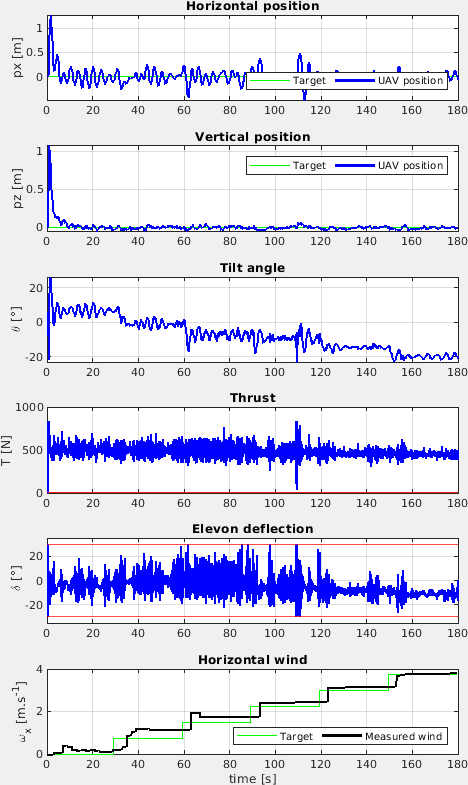
\includegraphics[width=0.6\columnwidth]{figures/exp.png}
     \caption{Résultats expérimentaux.}
     \label{fig_exp_centrage_arr}
 \end{figure}
Malgré quelques oscillations, le drone maintient sa position en dépit du vent, en inclinant convenablement l'angle de tangage. Les oscillations expérimentales sont absentes de nos simulations, ce qui suggère la présence de phénomènes non modélisés.
Nous observons également un comportement qui pourrait être important pour de futures recherches : le drone semble se stabiliser plus facilement le long de l'axe vertical que le long de l'axe horizontal. 

Comme prévu, lorsque le vent augmente, l'angle d'inclinaison diminue, ce qui modifie la poussée nécessaire et la déflexion des élevons. En effet, le vent génère de la portance sur les ailes, ce qui compense l'effet de la gravité, et donc la poussée nécessaire devient plus faible.
Pour chaque valeur de $w$, le modèle converge vers un équilibre, dont la caractérisation mathématique précise est détaillée dans \ref{sec:eq_vent}. Il est donc nécessaire d'étendre la robustesse du contrôleur en effectuant une optimisation multimodèle du contrôleur (décrite dans \ref{sec:h_inf6DOF_multi}). Il est également possible d'ajouter des degrés de libertés supplémentaires à  la structure du contrôleur afin de lui donner plus de degrés de liberté dans l'optimisation.

La vidéo de la maquette, avec les résultats expérimentaux est, disponible via le lien : \url{https://youtu.be/ce4_FUzeVzI}.



\section{Conclusion}
Nous avons décrit une maquette permettant de simuler le vol d'un drone convertible, DarkO, en soufflerie. L'objectif de cette maquette est de tester le système de contrôle sur une représentation fidèle de la dynamique longitudinale, tout en simulant la dynamique de translation. Nous avons également présenté un contrôleur linéaire du type retour dynamique de sortie basé sur une architecture proportionnelle-intégrale pour la stabilisation du vol stationnaire dans des conditions de vent constant. Les gains du contrôleur ont été obtenus à l'aide d'une optimisation non convexe. Les résultats des essais expérimentaux montrent qu'il est possible de stabiliser l'équilibre en vol stationnaire dans la plage de vitesse du vent testée. 

Toutefois, d'autres architectures de contrôle devraient être étudiées à l'avenir pour traiter les oscillations indésirables. Ces résultats indiquent qu'il est nécessaire de tester cette architecture de commande sur un modèle complet à six degrés de liberté.

\chapter{Méthode LMI }
\minitoc
\label{chap:LMI}

\section{Motivation}
\label{sec:motivationLMI}

Dans le chapitre précédemment, nous avons exploré la possibilité de stabiliser la dynamique longitudinale du drone à l'aide d'un contrôleur par retour de sortie. Les gains du contrôleur sont obtenus par une optimisation non-lisse basée sur des critères $H_{\infty}$. Nous proposons à présent d'étudier une manière différente de régler les gains du contrôleur, basée sur les inégalités linéaires matricielles.

Ce chapitre va permettre la mise en œuvre d'une formulation mathématique pour la synthèse du contrôleur basé modèle dans un cas pratique. Jusqu'à présent, cette approche a été testée et évaluée uniquement sur des cas théoriques \cite{Arzelier2018} avec des modèles dynamiques qui ne reflétaient pas les systèmes du monde réel. 

La méthode proposée pour contrôler le modèle de drone convertible étudié est basée sur la synthèse d'un contrôleur statique de sortie. Le contrôleur est obtenu en convertissant algorithmiquement le problème d'inégalités matricielles bilinéaires (BMI) non convexe en trois problèmes convexes auxiliaires :
\begin{itemize}
    \item un problème de retour d'état (SF),
    \item un problème d'injection de sortie (OI),
    \item un problème d'injection d'état (SI)
\end{itemize}

\nomenclature[]{\(BMI\)}{Inégalités matricielles bilinéaires  (\textit{Bilinear Matrix Inequalities})}
\nomenclature[]{\(SF\)}{Retour d'état  (\textit{State Feedback})}
\nomenclature[]{\(OI\)}{Injection de sortie (\textit{Output Injection})}
\nomenclature[]{\(SI\)}{Injection d'état (\textit{State injection})}


La résolution des problèmes (SF), (OI) et (SI) est une condition nécessaire à l'existence d'une solution pour le problème de retour statique de sortie. Par conséquent, la résolution de chacun des problèmes ci-dessus est abordée au moyen d'un algorithme en trois phases présenté à la section \ref{SOF Controller Synthesis}. Cet algorithme est mis en œuvre sur la dynamique augmentée de DarkO, laquelle est incorporée dans la boucle ouverte pour imposer une forme souhaitée semblable aux principes de la méthode de mise en forme de la boucle \cite{McFarlane1992}. Cela conduit à des garanties multiples, notamment en termes de performance (avec un gain élevé en boucle ouverte à basse fréquence) et en termes de robustesse (avec une stratégie de gain faible en boucle ouverte à haute fréquence), tout en satisfaisant à l'exigence de suivi de la référence. 

Les contrôleurs par retour statique de sortie résultant pour la dynamique augmentée seront validés par des simulations dans le domaine temporel. De plus, une validation sera également effectuée de manière expérimentale par le biais d'essais en vol réels, avec un modèle expérimental du drone DarkO. 

Le chapitre est organisé comme suit. La section \ref{SOF Controller Synthesis} détaille l'algorithme itératif déterministe pour la conception des contrôleurs par retour statique de sortie, ainsi que le processus d'augmentation du système. Dans la section \ref{resultLMI}, les résultats de la synthèse du contrôleur sont analysés au moyen de simulations dans le domaine temporel et d'expérimentations, en mettant en œuvre les lois de contrôle conçues directement sur le système réel. 



\section{Synthèse d'un contrôleur statique de sortie}
\label{SOF Controller Synthesis}

La synthèse d'un contrôleur statique de sortie pose un problème non convexe en raison des multiplications entre les variables de décision, ce qui entraîne des inégalités matricielles bilinéaires (BMI). Cette complexité rend le problème d'optimisation NP-difficile. 
En se référant à la formulation des BMI dans \cite{ebihara2015}, plusieurs reformulations équivalentes sont proposées dans \cite{Arzelier2018}, ce qui conduit à l'inégalité matricielle présentée dans \eqref{MainMatrixIneq}. La méthode proposée ici est extraite de \cite{ebihara2015}, s'appuyant notamment sur l'approche S-variable et les calculs duaux.



\begin{equation}
\centering
  \begin{gathered}
        \textcolor{blue}{P} \succ 0 \\
        He\left\{ \smallmat{
            0 & 0 & \textcolor{blue}{P}\\
            0 & 0 & 0\\
            \textcolor{blue}{P} & 0 & 0
        }\right\}
    \prec
    He\left\{\smallmat{
        \mathbb{I}\\
            -\left( \textcolor{blue}{\lambda} \smallmat{
                C\\
                0_{p-n,n}                
            } + \textcolor{blue}{M} \right)\\
            -A
    }
    \textcolor{blue}{S_1} +
    \smallmat{
        0\\
        \textcolor{blue}{S_2}\\
        B\textcolor{blue}{Z}
    }
    \smallmat{
        0 & \mathbb{I} & -\textcolor{blue}{H}^T
    }\right\}
    \end{gathered}
    \label{MainMatrixIneq}
\end{equation}
\begin{equation}
    \boldsymbol{F} = -\textcolor{blue}{Z} \textcolor{blue}{S_2}^{-1} \smallmat{ \mathbb{I}_p \\ 0_{n-p,p} }
    \label{GetF}
\end{equation}

Même si cette nouvelle reformulation est toujours non-convexe, elle permet d'obtenir un résultat. Si une solution est trouvée pour le système dans \eqref{MainMatrixIneq} avec $\textcolor{blue}{\lambda} = 1$, $\textcolor{blue}{M} = 0$ et $\textcolor{blue}{S_2}$ non singulière, alors nous pouvons calculer une matrice de gain $\boldsymbol{F}$ qui garantit la stabilité en boucle fermée (la preuve est disponible dans \cite{Arzelier2018}). Cette matrice de gain, qui n'est pas directement optimisée dans la synthèse convexe, est obtenue à l'aide de \eqref{GetF}. 

Cette preuve constitue l'objectif principal du processus d'optimisation. Relever les défis découlant de la nature non convexe du problème \ref{MainMatrixIneq} nécessite des avancées mathématiques et techniques spécifiques. La formulation mathématique introduite dans la littérature a donné des résultats théoriques initiaux prometteurs. L'algorithme, qui sera détaillé dans la sous-section suivante, sera appliqué à la dynamique du drone DarkO. L'analyse qui en résultera permettra de tirer des conclusions quant à l'efficacité de l'algorithme dans des scénarios d'essai pratiques.


\subsection{Algorithme déterministe itératif pour la conception de retour statique de sortie}
\label{3a}

Le problème de la synthèse de gain d'un retour statique de sortie se caractérise par sa nature intrinsèquement non convexe qui s'accompagne de difficultés de calcul liées aux problèmes NP-difficile. Ceci, associé à une complexité inhérente qui provient de l'impossibilité d'optimiser toutes les variables de décision simultanément, rend le processus de division du problème non-convexe en de multiples sous-problèmes convexes auxiliaires extrêmement attrayant. L'inégalité matricielle bilinéaire \eqref{MainMatrixIneq} sera utilisée pour traduire ces objectifs dans un cadre d'optimisation. Chaque objectif particulier est atteint en fixant de manière optimale une partie des variables de décision, tout en affinant le reste par un processus itératif. Pour concevoir le contrôleur, un algorithme en trois phases introduit dans \cite{Arzelier2018} sera mis en œuvre Fig. \ref{AlgoPhases}, lequel prend en entrée les matrices $\boldsymbol{A}$, $\boldsymbol{B}$, $\boldsymbol{C}$ de la dynamique linéarisée du système.

\begin{figure}[hbt]
    \centering
      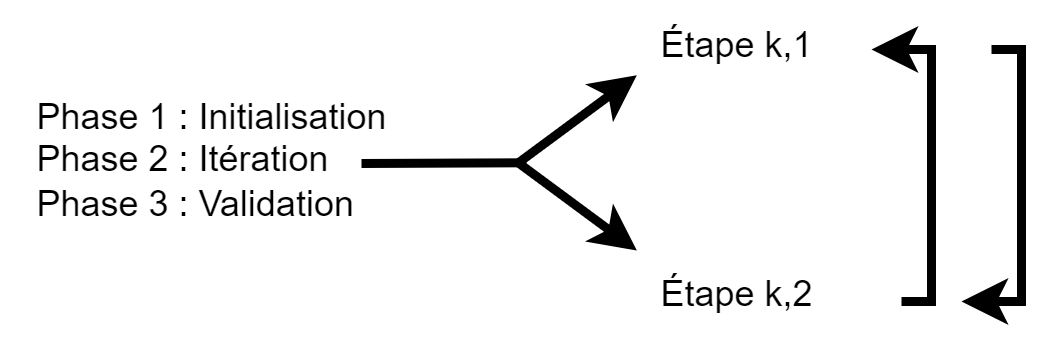
\includegraphics[width=0.6\columnwidth]{figures/LMIAlgo.png}
      \vspace{-0.2cm}\caption{Structure de l'algorithme d'optimisation.}
      \label{AlgoPhases}
\end{figure} 

\subsubsection{Phase d'initialisation} 
L'objectif de la première phase est essentiellement de fournir une estimation initiale pour un contrôleur matriciel de gain à retour d'état $\boldsymbol{K}$ qui stabilise la boucle fermée $\dot{\boldsymbol{x}}=(\boldsymbol{A}+\boldsymbol{B}\boldsymbol{K})\boldsymbol{x}$. Pour ce faire, la stratégie adoptée consiste à fixer les variables de décision \textcolor{blue}{$\lambda$, M, H} de \eqref{MainMatrixIneq} de la manière suivante :
\begin{equation}
    \begin{gathered}
        \textcolor{blue}{\lambda} = \lambda = 0, \quad
        \textcolor{blue}{M} = M_0 = \begin{pmatrix}
            C^{\circ}C\\
            {C^{\perp}}^T
        \end{pmatrix},\\
        \textcolor{blue}{H} = H_0 = J M_0^{-1}, \quad
        J = (-\mu-h)\mathbb{I},
    \end{gathered}
    \label{InitVariableFixing}
\end{equation} 
où $h$ est un scalaire positif et $-\mu$ est la partie réelle maximale des valeurs propres de $\boldsymbol{A}$. L'étude de faisabilité menée dans la phase d'initialisation est la suivante :

\begin{equation}
    \begin{gathered}
        \textcolor{blue}{P} \succ 0 \\
        He\left\{ \smallmat{
            0 & 0 & \textcolor{blue}{P}\\
            0 & 0 & 0\\
            \textcolor{blue}{P} & 0 & 0
       }\right\}
    \prec
    He\left\{\smallmat{
        \mathbb{I}\\
            -M_0 \\
            -\boldsymbol{A}
   }
    \textcolor{blue}{S_1} +
    \smallmat{
        0\\
        \textcolor{blue}{S_2}\\
        B\textcolor{blue}{Z}
    }
    \smallmat{
        0 & \mathbb{I} & -H_0^T
    }\right\}
    \end{gathered}
    \label{InitMatrixIneq} 
\end{equation} 

Si \eqref{InitMatrixIneq} est réalisable pour une combinaison de variables de décision \textcolor{blue}{$S_1$, $S_2$, Z} et pour le certificat de Lyapunov \textcolor{blue}{P}, alors une première estimation d'un gain de retour d'état stabilisant $\boldsymbol{K}$ est trouvée, et nous pouvons passer à la phase d'itération. En revanche, si aucune solution n'est trouvée, le paramètre $h$ est incrémenté de 1 et la phase d'initialisation est exécutée à nouveau. Cette phase résout les problèmes (SI) et (SF). Les résultats de cette phase sont les suivants :

\begin{equation}
    \begin{gathered}
        S_{1.0}=\textcolor{blue}{S_1},  \quad
        \hat{K}_0 = -\textcolor{blue}{Z} \textcolor{blue}{S_2}^{-1}, \quad
        K = -\textcolor{blue}{Z} \textcolor{blue}{S_2}^{-1} M_0
    \end{gathered}
    \label{OutputsInit}
\end{equation}

\subsubsection{Phase d'itération - Étape k,1}

Cette phase comprend deux étapes itératives. Dans la première étape, les variables d'optimisation $\lambda$ et $\boldsymbol{M}$ dans \ref{MainMatrixIneq} précédemment fixées lors de l'initialisation, sont maintenant traitées comme des variables de décision. Pour maintenir la convexité; la variable de marge \textcolor{blue}{$S_1$} est fixée à la valeur $S_{1,0}$ déterminée lors de la phase d'initialisation. Le système \eqref{Iter1MatrixIneq} est ensuite résolu.

\begin{equation}
\centering
    \begin{gathered}
        \textcolor{blue}{P} \succ 0, \quad \smallmat{
            (1-\textcolor{blue}{\lambda})\mathbb{I} & \textcolor{blue}{M^T}\\
            \textcolor{blue}{M} & \mathbb{I}
        } \geq 0 ,\quad \textcolor{blue}{\lambda} \geq 0 \\
        He\left\{ \smallmat{
            0 & 0 & \textcolor{blue}{P}\\
            0 & 0 & 0\\
            \textcolor{blue}{P} & 0 & 0
        }\right\}
    \prec
    He\left\{\smallmat{
            \mathbb{I}\\
            -\left( \textcolor{blue}{\lambda}
            \smallmat{
                C\\
                0_{p-n,n}
             } +
            \textcolor{blue}{M}
            \right) \\
            -A
    }
    S_{1,k-1} +
    \smallmat{
         0\\
        -\mathbb{I}\\
        B \hat{K}_{k-1}
    }
    \smallmat{
        0 & -\textcolor{blue}{S_2} & \textcolor{blue}{Y}^T
    }\right\}
    \end{gathered}
    \label{Iter1MatrixIneq}
\end{equation}

Dans \eqref{Iter1MatrixIneq}, deux inégalités matricielles apparaissent en plus de l'inégalité du certificat de Lyapunov et de l'inégalité \eqref{MainMatrixIneq}. Ces contraintes supplémentaires contribuent à la réalisation de l'objectif de la phase d'itération, qui consiste à trouver une solution pour \eqref{MainMatrixIneq} dans laquelle les variables $\lambda$ et $\boldsymbol{M}$ convergent respectivement vers 1 et 0, ce qui est une condition obligatoire pour atteindre l'objectif d'optimisation principal. Pour ce faire, la maximisation de $\lambda$ est définie comme un objectif dans le solveur d'optimisation. Une inégalité matricielle contraint la norme de $\boldsymbol{M}$ et la réduit à 0, à mesure que $\lambda$ augmente jusqu'à 1. La seconde inégalité est simplement une contrainte sur $\lambda$, ce dernier devant être positif.


Si une solution est trouvée pour \eqref{Iter1MatrixIneq} et si, pour cette solution, $1-\lambda$ est inférieur à une tolérance définie, cela signifie que l'on peut passer à la troisième et dernière phase, à savoir la validation. Les résultats de cette phase sont les suivants :

\begin{equation}
    \begin{gathered}
        \lambda_k=\textcolor{blue}{\lambda},  \quad
        M_k = \textcolor{blue}{M}, \quad
        H_k^T = \textcolor{blue}{S_2}^{-1} \textcolor{blue}{Y}^T
    \end{gathered}
    \label{OutputsIterStap2}
\end{equation}

Si ce n'est pas le cas, il y a une deuxième étape dans la phase d'itération.

\subsubsection{Phase d'itération - Étape k,2}


L'étape k,2 est relativement proche d'une étape d'initialisation. Comme pour la première phase, où \textcolor{blue}{$\lambda$, $M$} et \textcolor{blue}{$H$} ont été fixés comme entrées pour générer un gain de retour d'état stabilisateur $\boldsymbol{K}$, la deuxième étape fixe les mêmes variables de décision avec des valeurs mises à jour à partir de l'étape k,1.

Le problème d'optimisation à résoudre dans cette phase est le suivant :


\begin{equation}
\centering
    \begin{gathered}
        \textcolor{blue}{P} \succ 0 \\
        He\left\{ \begin{bmatrix}
            0 & 0 & \textcolor{blue}{P}\\
            0 & 0 & 0\\
            \textcolor{blue}{P} & 0 & 0
        \end{bmatrix}\right\}
    \prec
    He\left\{\begin{bmatrix}
           \mathbb{I}\\
                -\hat{M}(\textcolor{blue}{\alpha})\\
            -A
    \end{bmatrix}
    \textcolor{blue}{S_1} +
    \begin{bmatrix}
        0\\
        \textcolor{blue}{S_2}\\
        B\textcolor{blue}{Z}
    \end{bmatrix}
    \begin{bmatrix}
        0 & \mathbb{I} & -H_k^T
    \end{bmatrix}\right\}
    \end{gathered}
    \label{Iter2MatrixIneq}
\end{equation}
\begin{equation}
    \begin{gathered}
        \hat{M}(\textcolor{blue}{\alpha}) = \left((1+\textcolor{blue}{\alpha} (\lambda_k-1))
        \begin{bmatrix}
            C \\
            0_{p-n,n}
        \end{bmatrix}
        +
        \textcolor{blue}{\alpha} M_k\right)
    \end{gathered}
    \label{Artificiu2}
\end{equation}

Lors de cette étape, un nouveau terme, $\hat{M}(\textcolor{blue}{\alpha})$ apparaît, dépendant d'une nouvelle variable de décision $\textcolor{blue}{\alpha}$. L'objectif est de minimiser \textcolor{blue}{$\alpha$} à l'aide de la méthode de bissection, en convertissant le problème non convexe en un problème convexe. Idéalement, \textcolor{blue}{$\alpha$} converge vers 0, signalant la fin de cette phase d'itération et la progression vers la phase de validation finale. Si $\alpha \approx 0$ selon une certaine tolérance, \eqref{Artificiu2} se simplifie en \eqref{Artificiu3}. Par conséquent, les valeurs des variables de décision pour la solution de \eqref{Iter2MatrixIneq} lors l'étape k,2 sont identiques à la solution de \eqref{MainMatrixIneq}, laquelle est résolue pour $\lambda = 1$ et $\boldsymbol{M} =0$. Cette solution permet le calcul d'un contrôleur par retour de sortie statique stabilisant.

\begin{equation}
    \begin{gathered}
        \hat{M}(\alpha) = \left((1+\alpha (\lambda_k-1))
        \begin{bmatrix}
            C \\
            0_{p-n,n}
        \end{bmatrix}
        + 
        \alpha M_k\right)
        \stackrel{\alpha \approx 0 }{=}
        \begin{bmatrix}
            C \\
            0_{p-n,n}
        \end{bmatrix}
    \end{gathered}
    \label{Artificiu3}
\end{equation}

Si, à l'étape k,2, $\alpha$ n'est pas inférieure à la tolérance fixée, l'algorithme commence une nouvelle étape d'itération à k,1. Les résultats de la phase actuelle sont les suivants :

\begin{equation}
    \begin{gathered}
\alpha_k=\textcolor{blue}{\alpha}  \quad
        \hat{K}_{k-1} = -\textcolor{blue}{Z} \textcolor{blue}{S_2}^{-1} \quad
        S_{1,k} = \textcolor{blue}{S_1}
    \end{gathered}
    \label{OutputsIterStap1}
\end{equation}

\subsubsection{Phase de validation}
Dans les cas où l'étape d'itération fournit des solutions pour lesquelles $\boldsymbol{\lambda} = 1 $ et $\boldsymbol{M} = 0$, une phase de validation n'est pas nécessaire car le contrôleur peut être calculé directement. 

En pratique, l'algorithme quitte la phase d'itération avec des solutions $\boldsymbol{\lambda} \approx 1$ et $\boldsymbol{M} \approx 0$, en raison des limites des solveurs d'optimisation et des précisions numériques. Dans ces cas, les conditions pour atteindre l'objectif d'optimisation principal ne sont pas exactement remplies. Par conséquent, une phase de validation est nécessaire. Le problème à résoudre est défini par \eqref{ValidMatrixIneq}, où les variables sont fixées $\boldsymbol{\lambda} = 1$ et $\boldsymbol{M} = 0$ et $\boldsymbol{H}$ est fixé à $\boldsymbol{H_k}$ (obtenu au cours de la phase d'itération). Si une solution est trouvée, la matrice de gain $\boldsymbol{F}$ peut être construite avec \eqref{GetF}, ce qui garanti la stabilité la boucle fermée $(\boldsymbol{A}+\boldsymbol{B}\boldsymbol{F}\boldsymbol{C})$. Cette dernière phase fournit la solution aux objectifs (OI) et (OF). 

\begin{equation}
\centering
    \begin{gathered}
        \textcolor{blue}{P} \succ 0 \\
        He\left\{ \begin{bmatrix}
            0 & 0 & \textcolor{blue}{P}\\
            0 & 0 & 0\\
            \textcolor{blue}{P} & 0 & 0
        \end{bmatrix}\right\}
    \prec
    He\left\{\begin{bmatrix}
            \mathbb{I}\\
                -\begin{bmatrix}
                    C \\
                    0_{p-n,n}
                \end{bmatrix}\\
            -A
    \end{bmatrix}
    \textcolor{blue}{S_1} +
    \begin{bmatrix}
        0\\
        \textcolor{blue}{S_2}\\
        B\textcolor{blue}{Z}
    \end{bmatrix}
    \begin{bmatrix}
        0 & \mathbb{I} & -H^T
    \end{bmatrix}\right\}
    \end{gathered}
    \label{ValidMatrixIneq}
\end{equation}


\subsection{Architecture de commande}
\label{3b}


L'architecture de contrôle du drone DarkO est conçue pour le stabiliser en vol stationnaire, avec et sans perturbations externes. Par exemple, pour contrer un vent de face affectant la vitesse linéaire le long des axes $x_{[b]}$ et $z_{[b]}$ et générant un moment autour de l'axe $y_{[b]}$, le schéma de commande utilise les ailerons et les hélices de manière symétrique pour générer un moment et une force compensatoires. Une action intégrale est employée pour contre-balancer la force le long de l'axe $z_{[b]}$, assurant une convergence asymptotique vers la force désirée en utilisant deux intégrateurs, un pour les moteurs et un pour les élevons.


La synthèse d'un contrôleur par retour de sortie statique pour la dynamique de DarkO augmentée s'inspire de \cite{SYRMOS1997125} où il est montré qu'un retour de sortie dynamique d'ordre $q \leq n$ (système d'ordre $n$), peut être converti en un retour de sortie statique à travers l'augmentation de l'espace d'état. Dans notre cas, des termes dynamiques tels que des intégrateurs et des filtres sont ajoutés à la dynamique du système, ce qui donne un espace d'état augmenté pour lequel une loi de bouclage statique composée d'une matrice de gain statique sera synthétisée. L'architecture mise en œuvre, présentée à la figure \ref{Plant Augmentation}, est une reformulation de la loi de contrôle présentée dans le chapitre \ref{chap:3DOF}. Elle se compose du bloc dynamique linéarisé du drone DarkO \eqref{eq:linearized} avec les matrices $\boldsymbol{A}_{0}$ \eqref{matrice_A} et $\boldsymbol{G}_{0}$ \eqref{matriceG0}, du bloc de saturation pour les deux hélices et les deux élevons, comme présenté dans la section \ref{sec:saturation}. La matrice de sélection des sorties élimine la mesure de l'état de l'angle de tangage, $\theta$.

\begin{figure}[hbt]
    \centering
    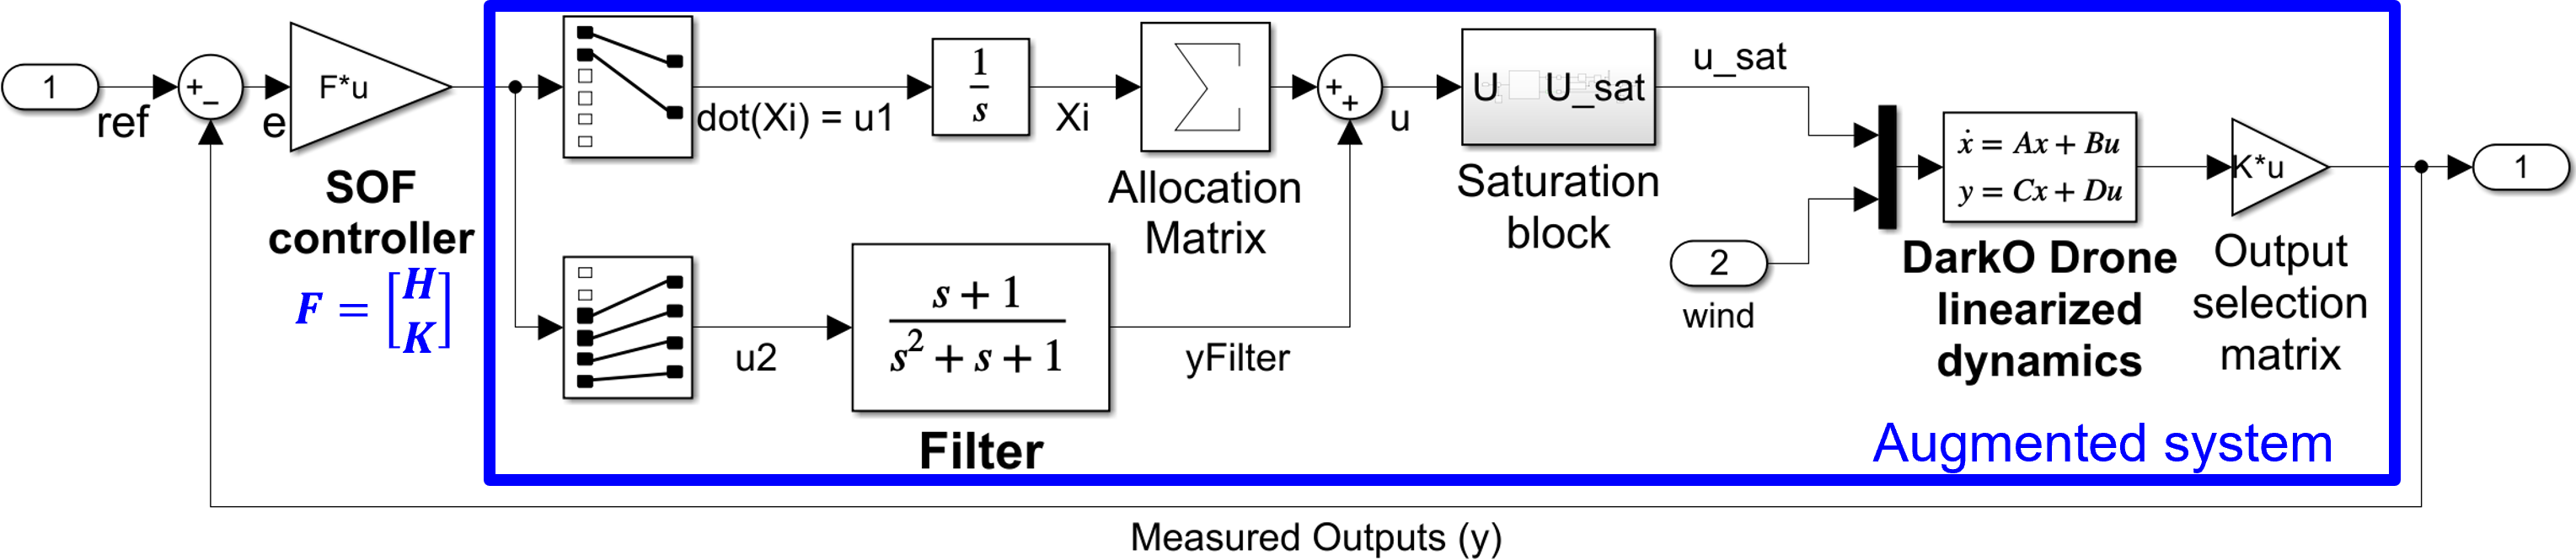
\includegraphics[width=0.9\columnwidth]{figures/AugWindFinal.png}
    \vspace{-0.3cm}\caption{Augmentation du système.}
    \label{Plant Augmentation}
\end{figure}


Pour la conception du contrôle, une structure de contrôleur de type PI est employée pour minimiser l'erreur statique et améliorer le rejet des perturbations externes. Pour ce faire, nous ajoutons des filtres pré-compensateurs à l'entrée du système, sur la base de la méthodologie de mise en forme en boucle ouverte \cite{McFarlane1992}. Un intégrateur est ajouté pour assurer la performance (gain élevé) à basse fréquence, ce qui correspond à la spécification de suivi. De même, un filtre de deuxième ordre est ajouté pour assurer que le contrôleur soit strictement propre et robuste en ce qui concerne les dynamiques négligées grâce à un comportement d'atténuation. La fréquence de coupure du filtre est fixée à environ \SI{5}{\hertz} pour s'aligner sur la dynamique de la boucle fermée et rejeter le bruit dans les signaux mesurés. Pour limiter le nombre d'intégrateurs à 2 (un qui génère la commande d'intégration pour les deux hélices et l'autre pour les deux élevons), les sorties du bloc intégrateur sont doublées par une matrice d'allocation $\Sigma$. L'implémentation d'un filtre de second ordre présente l'avantage supplémentaire d'éviter un terme de transmission directe, qui peut amplifier les bruits indésirables des capteurs. La matrice de gain $\boldsymbol{F}$ comprend les matrices de gain $\boldsymbol{H}$ et $\boldsymbol{K}$ respectivement pour l'action intégrale et proportionnelle. Les équations et la représentation de l'espace d'état du système augmentée se trouvent dans \eqref{AugEq1}.

\begin{equation}
\centering
    \begin{gathered}
        \dot{x}_i = u_1, \\
        u = \Sigma x_i + y_{filter} = \Sigma x_i + Filter \cdot u_2 \\
        \dot{x} = Ax + Bu = Ax + B(\Sigma x_i + y_{filter}) = Ax + B\Sigma x_i + B C x_{filter}, \\
        \Sigma =
        \smallmat{
            1 & 0 \\ 1 & 0 \\ 0 & 1 \\ 0 & 1   
        }, \quad \quad
        \smallmat{
            u_1 \\ u_2   
        }
        = F e = F \left(\smallmat{ref \\ \mathbb{0}_{8\times 1} }-y\right)  ,\\
        \smallmat{
            \dot{x} \\ \dot{x_c} \\ \dot{x}_{filter}
        } =
        \smallmat{
            A & B \Sigma & B C_{filter} \\
            0 & 0 & 0 \\
            0 & 0 & A_{filter} 
        }
        \smallmat{
            x \\ x_c \\ x_{filter}
        }
        +
        \smallmat{
            0 & 0 \\ 1 & 0 \\ 0 & B_{filter}
        }
        \smallmat{
            u_1 \\ u_2
        },  \\
        y = \smallmat{
            C & 0 & 0
        }
        \smallmat{
            x \\ x_c \\ x_{filter}
        },
    \end{gathered}
    \label{AugEq1}
\end{equation}
où $\boldsymbol{x_i} \in \mathbb{R}^{2}$ sont les états des intégrateurs,  $\boldsymbol{x_f} \in \mathbb{R}^{4}$ sont les états des filtres, $\boldsymbol{r} \in \mathbb{R}^{3}$ est le signal de référence, $\boldsymbol{y} \in \mathbb{R}^{11}$ est la sortie mesurée et $\boldsymbol{u}\in \mathbb{R}^{4}$ est l'entrée du système.

\section{Résultats}
\label{resultLMI}
\subsection{Résultats de simulation}

L'approche de la section \ref{3a} a été appliquée au système augmenté de la section \ref{3b}, en se concentrant sur la dynamique linéarisée pour une vitesse de vent nulle (scénario de vol stationnaire). On a ainsi obtenu quatre contrôleurs stabilisateurs pour $h=12, 13, 14 \text{ et } 15$, $h$ variant entre 1 et 40. Plusieurs itérations avec différentes valeurs de $h$, servant de points d'initialisation pour l'algorithme d'optimisation, sont nécessaires pour améliorer la probabilité de convergence.

La figure \ref{HKStepRes_a} montre la réponse temporelle en boucle fermée des quatre contrôleurs, avec des variations de consigne sur l'axe $x$ à 5 s, l'axe $y$ à 90 s et l'axe $z$ à 40 s. Tous les contrôleurs stabilisent efficacement la dynamique en boucle fermée et suivent les références de position selon les trois axes. La réponse est lente sur les axes $x$ et $z$ et rapide sur l'axe $y$. Cela est dû à la capacité d'actionnement et l'utilisation différentielle des moteurs. De plus, une variation de consigne sur un axe n'entraîne pas de changement significatif sur les deux autres axes, ce qui indique un fort découplage entre les états de position. En outre, les actionneurs n'ont jamais été saturés.


\begin{figure}[hbt]
    \centering
   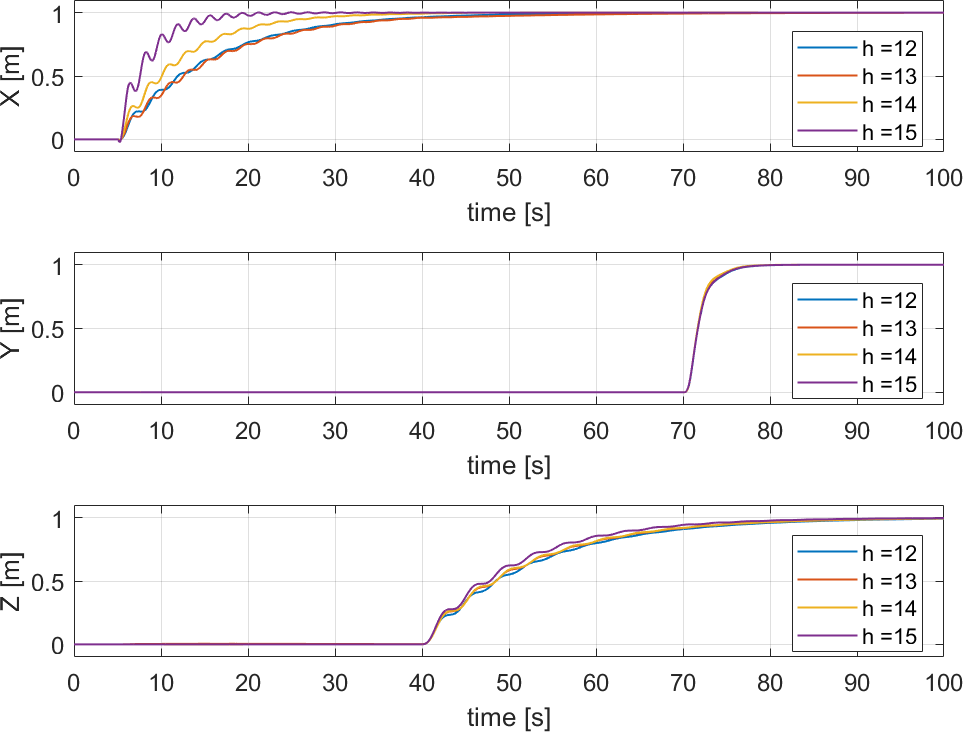
\includegraphics[width=0.9\columnwidth]{figures/stepResponse.png}
    \caption{Réponse du bouclage \eqref{AugEq1} avec une dynamique linéaire \eqref{eq:linearized}.}
    \label{HKStepRes_a}
\end{figure}

Le premier graphique de la figure \ref{thetanowind} montre que l'angle d'incidence $\theta$ subit des oscillations croissantes au fur et à mesure que h augmente. Bien que l'angle d'incidence $\theta$ ne soit pas directement contrôlé, il converge naturellement vers 0 lorsque les autres états se stabilisent, ce qui indique un vol stationnaire sans vent. Le second graphique montre que pour une dynamique linéarisée autour d'une vitesse de vent spécifique, $\theta$ converge vers une valeur non nulle, compensant les perturbations externes.

\begin{figure}[hbt]
    \centering
    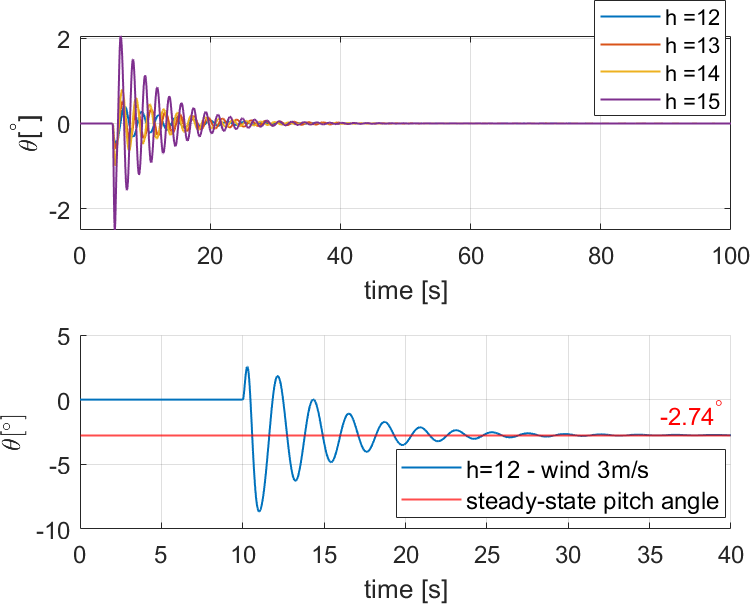
\includegraphics[width=0.9\columnwidth]{figures/windThetafinalhopeCrop.png}
    \vspace{-0.3cm}\caption{Réponse temporelle de l'angle d'incidence $\theta$ en boucle fermée.}
    \label{thetanowind}
\end{figure}

Les équations \eqref{Kstructure1} et \eqref{Kstructure2} présentent les gains du contrôleur synthétisés $\boldsymbol{F}$ (bloc illustré dans \ref{Plant Augmentation}) comprenant les gains matriciels $\boldsymbol{H}$ et $\boldsymbol{K}$ pour h=12 et une dynamique linéarisée à une vitesse de vent nulle. En examinant plus attentivement la matrice de gain $\boldsymbol{K}$ qui produit quatre signaux de commande utilisés pour la commande asymétrique ou symétrique des actionneurs du drone, on peut observer que les lignes 1 et 2 (qui génèrent une commande de poussée sur les deux hélices) ainsi que les lignes 3 et 4 (qui génèrent une commande d'angle de déflexion pour les deux élevons) sont soit presque égales, soit opposées, à quelques exceptions près. Ce modèle a émergé naturellement du processus d'optimisation sans aucune contrainte, reflétant un alignement intuitif et cohérent avec la dynamique du drone.

\begin{equation}\label{Kstructure1}
\boldsymbol{H}=
\smallmat{
  3.5e\shortminus6 & \shortminus3.0e\shortminus7 &  1.5e\shortminus2 & \shortminus6.9e\shortminus6 & \shortminus7.4e\shortminus6 &  4.4e\shortminus1 & 1.8e\shortminus4 &  1.1e\shortminus4 & \shortminus8.4e\shortminus5 & \shortminus8.6e\shortminus5 & \shortminus2.3e\shortminus4\\
  \shortminus2.0e\shortminus2 & \shortminus7.5e\shortminus6 &  1.6e\shortminus5 & \shortminus2.0e\shortminus1 &  4.4e\shortminus5 & \shortminus1.1e\shortminus4 & \shortminus9.2e\shortminus5 & \shortminus9.1e\shortminus5 &  7.4e\shortminus6 &  7.6e\shortminus1 & \shortminus3.9e\shortminus5}
\end{equation}
 \begin{equation}\label{Kstructure2}
\boldsymbol{K}=
\smallmat{
  7.6e\shortminus3 & \shortminus2.0e+1 &  9.9 &  3.1e\shortminus2 & \shortminus4.5e+1 &  8.2e+1 &\shortminus3.1e+2 & \shortminus3.1e+2 &  6.4e\shortminus1 &  3.0e\shortminus3 & \shortminus1.0e+2 \\
  5.4e\shortminus3 &  2.0e+1 &  9.9 &  8.8e\shortminus3 &  4.5e+1 &  8.2e+1 & 3.1e+2 &  3.1e+2 & \shortminus6.5e\shortminus1 & \shortminus1.9e\shortminus3 &  1.0e+2\\
  \shortminus4.2 & \shortminus3.2e\shortminus1 &  8.7e\shortminus3 & \shortminus4.5e+1 & \shortminus4.4e\shortminus1 & \shortminus3.1e\shortminus2 & \shortminus1.2e+1 &  1.6 & \shortminus3.1e+1 &  3.9e+1 & \shortminus1.6 \\
  \shortminus4.2 &  3.2e\shortminus1 &  4.8e\shortminus3 & \shortminus4.5e+1 &  4.3e\shortminus1 &  3.3e\shortminus2 & 1.2e+1 & \shortminus1.7 &  3.1e+1 &  3.9e+1 &  1.6}
\end{equation}



\subsection{Résultats expérimentaux}

Pour la validation expérimentale, les contrôleurs ont été testés sur le modèle réel de drone DarkO construit à l'ENAC Fig. \ref{DarkO1}. Les essais en vol ont eu lieu dans la volière de l'ENAC, équipée d'un système de capture de mouvement Optitrack fournissant des données de position et d'attitude à \SI{40}{\hertz}, éliminant ainsi le besoin d'un capteur GPS. La vitesse est obtenue par une différence finie. Des algorithmes de fusion de données, y compris des filtres invariants, ont combiné les données d'Optitrack (position, vitesse et attitude) et de l'unité IMU du drone DarkO pour améliorer l'estimation de l'état. Cette estimation est utilisée pour créer le vecteur de sortie $\boldsymbol{y}$, entrée de la loi de contrôle \eqref{AugEq1}. Compte tenu de l'architecture de la boucle de contrôle, l'estimation doit être de très bonne qualité avec le délai le plus court possible.

La nature modulaire de Paparazzi permet d'utiliser l'implémentation existante du filtre invariant pour estimer le vecteur d'état de DarkO et d'ajouter un module de stabilisation basé sur la loi de contrôle décrite ci-dessus (voir \ref{3b}). L'autopilote échantillonne les lois de commande et de contrôle à \SI{500}{\hertz}, générant des commandes de contrôle appropriées pour réaliser les manœuvres de vol souhaitées et stocker toutes les données en vue d'une analyse a posteriori.

\begin{figure}[ht]
    \centering
    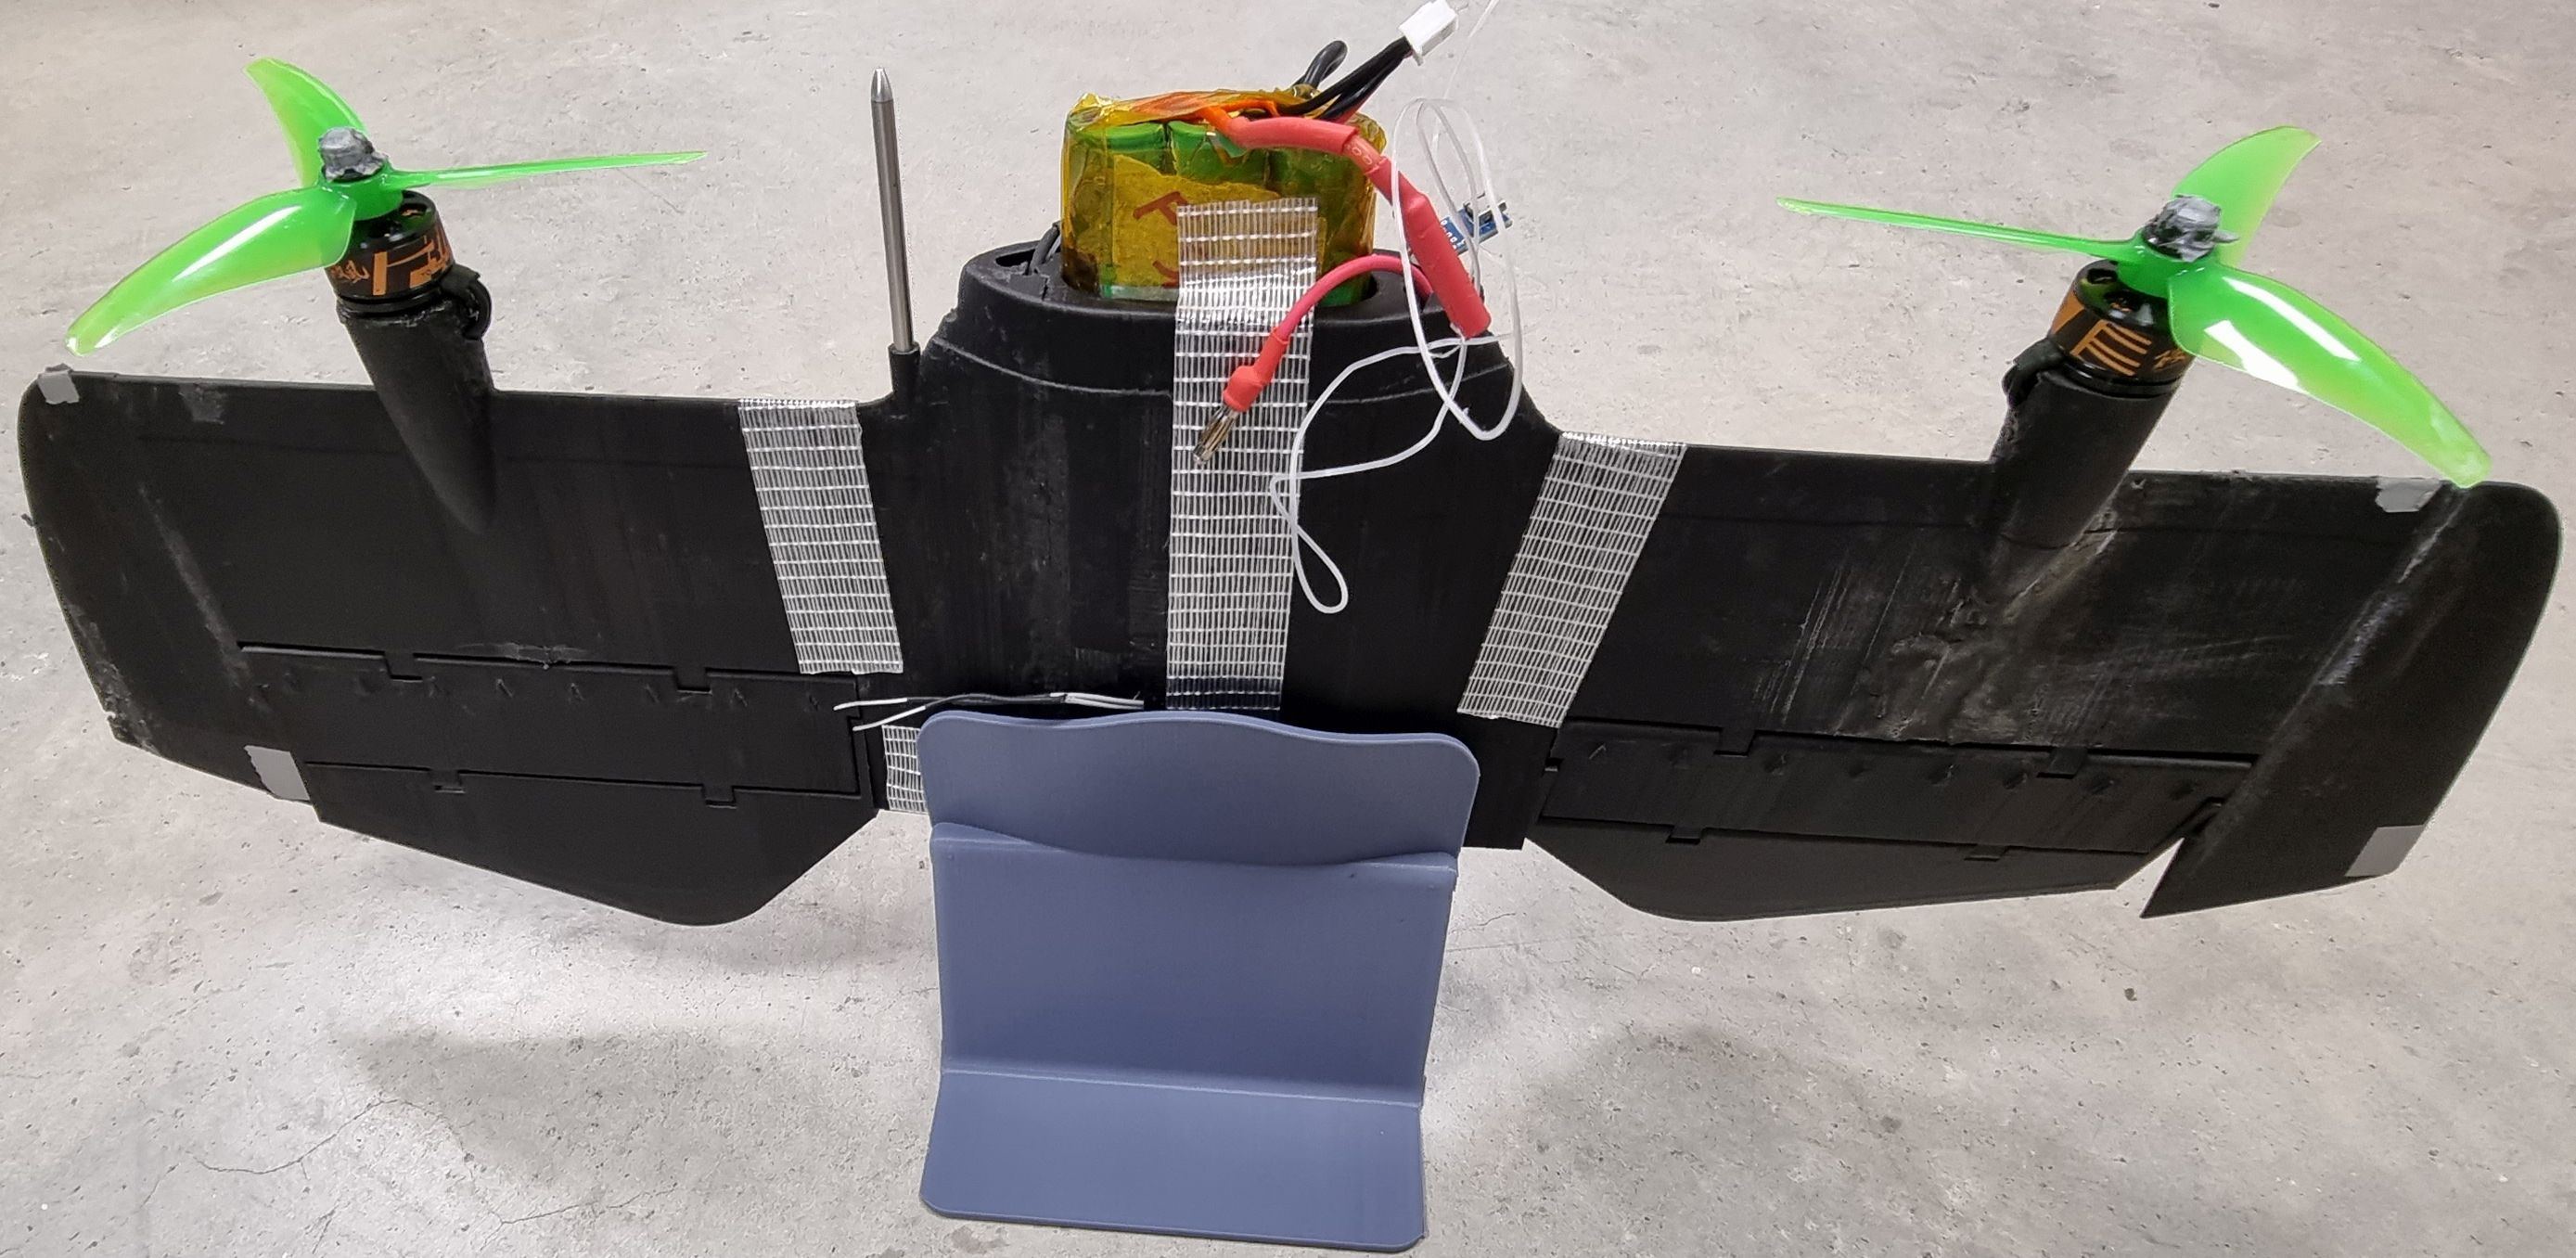
\includegraphics[width=0.8\columnwidth]{figures/DarkOModelfinal.jpg}
   \vspace{-0.2cm}\caption{Modèle expérimental du drone DarkO.}
    \label{DarkO1}
\end{figure}
\begin{figure}[ht]
    \centering
    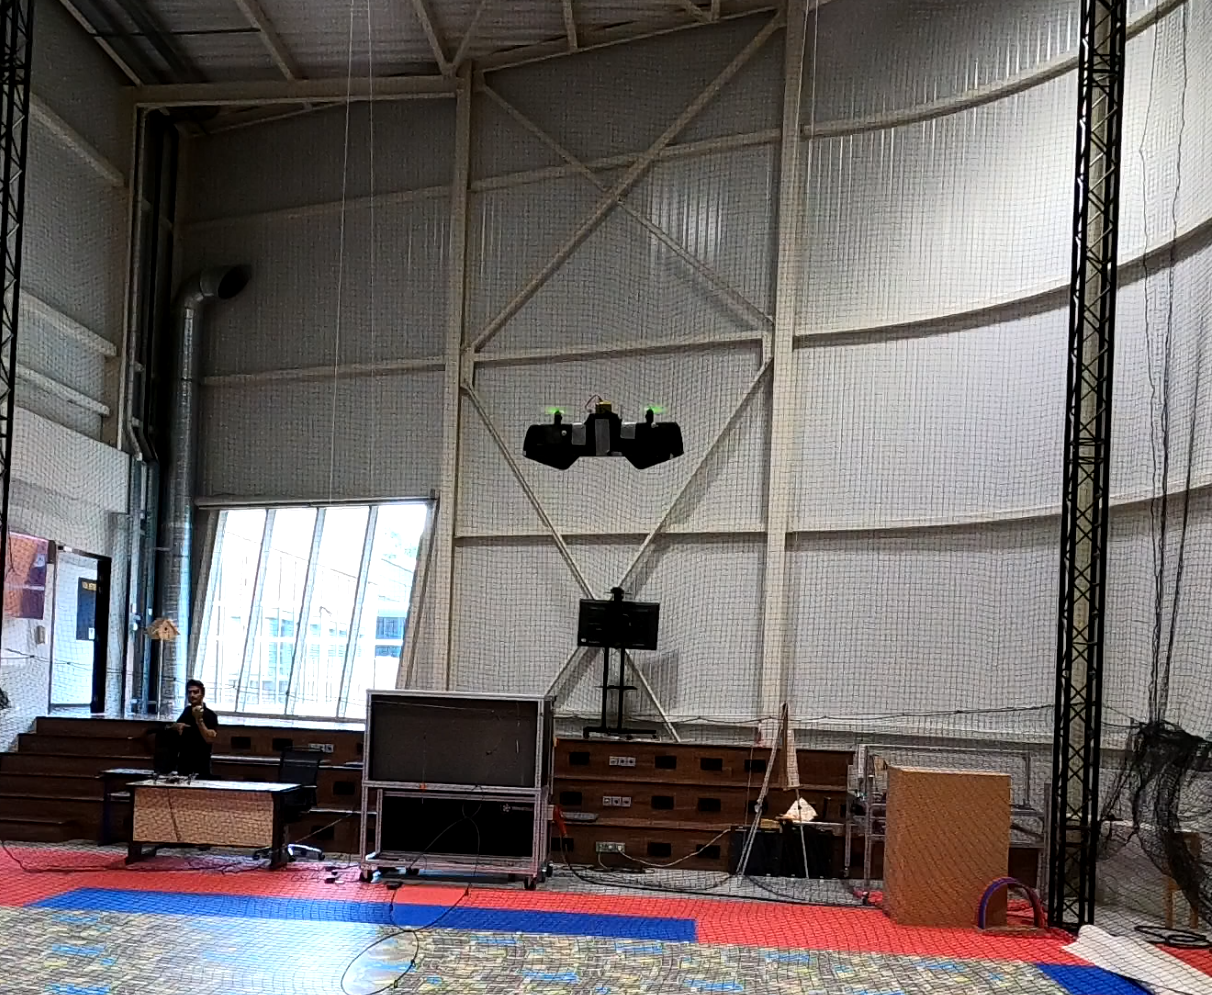
\includegraphics[width=0.8\columnwidth]{figures/DarkOFlighthope.png}
    \vspace{-0.2cm}\caption{DarkO lors d'un vol expérimental.}
    \label{DarkO2}
\end{figure}

Les essais expérimentaux suivants constituent les expérimentations réalisées dans la volière de l'ENAC où des contrôleurs ont été obtenu avec des méthodes de synthèse basées sur une modélisation du drone convertible. Les vols précédents pour ce type de drone utilisaient des conceptions de contrôle combinées basées sur des modèles et des capteurs, comme les algorithmes INDI. Chaque vol commence par le décollage du drone et sa stabilisation à une position de référence à l'aide d'un contrôleur INDI. Après avoir atteint la position de vol stationnaire souhaitée, le contrôleur INDI est remplacé par le contrôleur par retour de sortie. La figure \ref{Dabbene_Flight_Test } montre les résultats des essais en vol de l'un des quatre contrôleurs synthétisés. La figure \ref{DarkO2} représente le drone DarkO pendant son vol d'essai. Les quatre contrôleurs ont été testés et validés sur le système réel, démontrant une performance stable et un suivi de position précis sur les trois axes.


\begin{figure}[h]
    \centering
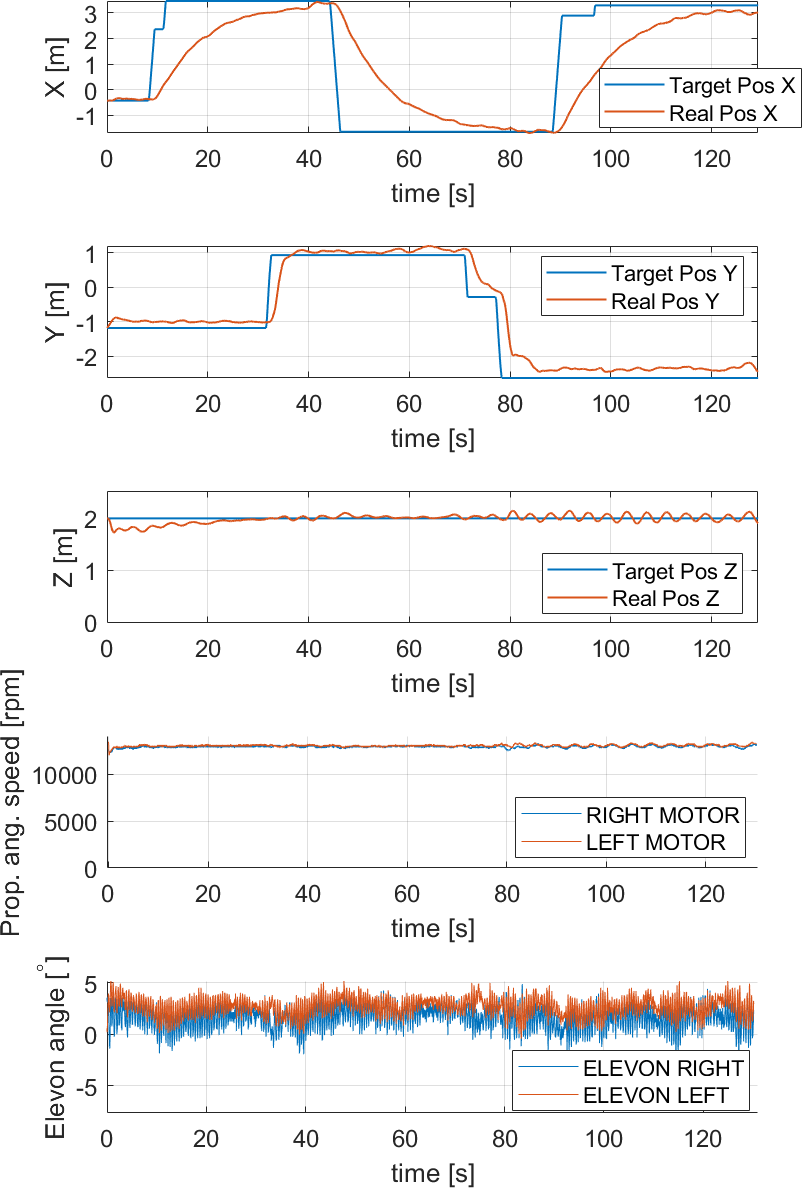
\includegraphics[width=1\columnwidth]{figures/realflight_z_adjust_x_adjust_final_HopeCrop.png}
   \vspace{-0.5cm}\caption{Réponse expérimentale en boucle fermée et entrée de commande pour $h = 12$.}
    \label{Dabbene_Flight_Test }
\end{figure}

Comme cela a également été observé dans les simulations, sur les axes $x$ et $z$, la réponse temporelle est relativement élevée alors que sur l'axe $y$, la réponse temporelle est considérablement plus rapide, en raison de l'actionnement différentiel important sur cet axe soutenu par la dynamique rapide de l'actionneur. Sur l'axe $z$, le passage du contrôleur INDI au contrôleur synthétisé entraîne une descente verticale relativement importante du drone. Par conséquent, un réglage et une modélisation supplémentaire doivent être effectués afin de corriger les valeurs d'initialisation de l'état et de l'entrée de commande correspondant au point d'équilibre \eqref{eq:equilibria}. La dynamique du drone sur l'axe $z$ est caractérisée par de petites oscillations autour de la position de référence, qui peuvent également être observées dans le signal de commande des vitesses angulaires des hélices, illustré à la figure \ref{Dabbene_Flight_Test}. Ces oscillations réduites sont dues au fait que la dynamique de l'actionneur n'est pas prise en compte dans la loi de commande. Il convient de noter que l'objectif premier de l'algorithme d'optimisation est de parvenir à une stabilisation en boucle fermée, sans tenir compte des critères de performance ou de robustesse. Au cours des vols expérimentaux, le contrôleur n'a pas saturé les actionneurs (voir la figure \ref{Dabbene_Flight_Test}).



\section{Conclusion du Chapitre \ref{chap:LMI}}

Un algorithme d'optimisation convexe, utilisant le cadre LMI et la théorie de la stabilité de Lyapunov, a été employé pour synthétiser des contrôleurs à retour de sortie statique pour le modèle de drone convertible DarkO. Cette technique de synthèse basée sur le modèle a permis de stabiliser efficacement la dynamique en boucle fermée du système, assurant une réponse temporelle satisfaisante et un suivi de la référence sans saturation des actionneurs. Malgré une modélisation incomplète des phénomènes non linéaires, les contrôleurs ont démontré leur robustesse lors des premières démonstrations expérimentales sur le modèle de drone DarkO. Avec les matrices de gain du contrôleur conçues et la structure de la loi de commande, des vols expérimentaux ont été menés avec succès pour le vol stationnaire et le suivi de la trajectoire. Ce résultat constitue une solide preuve de concept pour la loi de commande développée en termes de performance et de robustesse.
Il est maintenant nécessaire de s'intéresser à l'impact du vent sur l'architecture du drone et aux impacts sur l'obtention des gains du contrôleur.

\chapter{Modélisation d'un drone à aile libre rotation libre}
\minitoc

\section{Design et modélisation d'un drone : Colibri}
\section{Design and modelling of Colibri UAV}\label{sec:model}
The Colibri drone is derived from a tail-sitter drone with a wing that generates lift during the forward flight. This wing has several actuators: four motors $u_{i}, ~i = 1,2,3,4$ and two elevons $\delta_{\text{l}}$ and $\delta_{\text{r}}$. We can define the control vector $u_{\text{W}}$ of the wing based on Figure~\ref{fig:world_body} as $u_{\text{W}} = [u_{1}~u_{2}~u_{3}~u_{4}~\delta_{\text{l}}~\delta_{\text{r}}]^\top$. A fuselage linked by a pivot is secured at the aerodynamic centre of the wing. This fuselage supports the autopilot, the battery, a motor and a tail to keep it horizontal. In Figure \ref{fig:world_body}, all the aerodynamic control surfaces are shown in pink and the propellers are shown in green.
There are three reference frames attach to the drone. (I) is a NED inertial reference frame (or world frame) linked to the earth's surface, (W) is a wing reference frame attached to the drone wing and (F) is a fuselage reference frame attached to the drone fuselage.
% Deux configurations sont étudiées pour la position des moteurs. 

% \begin{figure}[h]
% \centering
%     \includegraphics[width=1\columnwidth,angle=0]{picture/colibriH.jpg}
%     \caption{The Colibri convertible UAV, H version. }
%     \label{fig:colibri_h}
% \end{figure}

% L'architecture en H offre un actionnement important 

% \begin{figure}[h]
% \centering
%     \includegraphics[width=1\columnwidth,angle=0]{picture/ColibriV2.png}
%     \caption{The Colibri convertible UAV, motor on the wing. }
%     \label{fig:colibriv2}
% \end{figure}

\begin{figure}[h]
\centering
    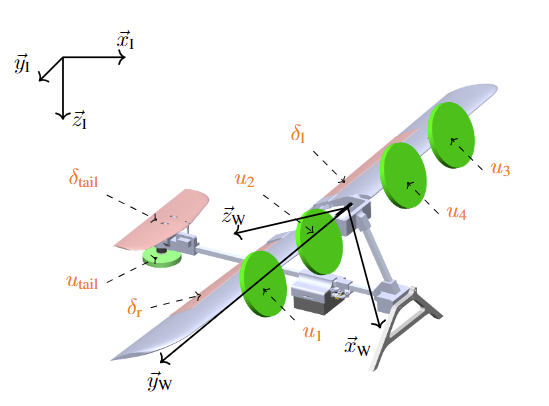
\includegraphics[width=1\columnwidth,angle=0,trim={0 0 0 0.5cm},clip]{figures/wold_body.png}
    \caption{Inertial (I) and wing (W) reference frames and the Colibri architecture. }
    \label{fig:world_body}
\end{figure}
% \todo{he reference frames could be introduced
% and detailed at the beginning of the section}

Some of the characteristic dimensions are shown in Table~\ref{tab:pars}. Note that the motors are positioned symmetrically on the wing, which means that the position can be described by focusing on one side. 
\begin{table}[ht]
  \centering
    \begin{tabular}{|l|c|c|}
      \hline
      \multicolumn{1}{|c|}{Parameter} & Value & Units  \\
      \hline
      $m_{\text{W}}$ (wing mass)  & 0.53& \SI{}{\kilogram} \\
      \hline
      $m_{\text{F}}$ (fuselage mass)  & 1.17& \SI{}{\kilogram} \\
      \hline
    %   $b$ (wingspan)  & 1.17 & \SI{}{\meter} \\
    %   \hline
    %   $c$ (aerodynamic cord)  & 0.150 & \SI{}{\meter} \\
    %   \hline
    %   $S$ (wing area) & 0.1537 & \SI{}{\square\meter}\\
    %   \hline
    %   $S_{\text{wet}}$ (wet area) & 0.0813 & \SI{}{\square\meter}\\
    %   \hline
    %   $S_{\text{p}}$ (propeller area) & 0.0182 & \SI{}{\square\meter}\\
    %   \hline
      $J_{\text{W}}=diag(J_{x}^{\text{W}}, J_{y}^{\text{W}}, J_{z}^{\text{W}})$ & \!\! $\diag(0.1677,0.0052,0.1634)$\!\! & \SI{}{\kilogram\square\meter}\\
      \hline
      $J_{\text{F}}=diag(J_{x}^{\text{F}}, J_{y}^{\text{F}}, J_{z}^{\text{F}})$ & \!\! $\diag(0.0191,0.0161,0.0343)$\!\! & \SI{}{\kilogram\square\meter}\\
      \hline
      $k_{\text{f}}$ (propeller thrust coeff.) & 1.7800e-8 & \SI{}{\kilogram\meter}\\
      \hline
    %   $k_{\text{m}}$(propeller torque coeff.) & 2.1065e-10 & \SI{}{\kilogram\square\meter}\\
    %   \hline
    %   $p_{z}^{int}$ (propeller $z$ location) & 0.037 & \SI{}{\meter}\\
    %   \hline
    %   $p_{y}^{int}$ (propeller $y$ location) & 0.145 & \SI{}{\meter}\\
    %   \hline
    %   $p_{z}^{ext}$ (propeller $z$ location) & 0.028 & \SI{}{\meter}\\
    %   \hline
    %   $p_{y}^{ext}$ (propeller $y$ location) & 0.325 & \SI{}{\meter}\\
    %   \hline
    %   $\xi_{\text{f}}$ (elevons lift coeff.) & 0.2 & --\\
    %   \hline
    %   $\xi_{\text{m}}$ (elevons torque coeff.) & 1.4 & --\\
    %   \hline
    %   $\rho$ (air density) & 1.225 & \SI{}{\kilogram\per\cubic\meter}\\
    %   \hline
    %   $C_{\text{d0}}$ (drag coeff.) & 0.1644 & --\\
    %   \hline
    %   $C_{\text{l0}}$ (lift coeff.) & 5.4001 & --\\
    %   \hline
       $d_{\text{M}O_{\text{W}}}$  & $[0.383,0,-0.167]^\top$ & \SI{}{\meter}\\
      \hline
       $d_{\text{G}O_{\text{W}}}$  & $[0.052,0,-0.171]^\top$ & \SI{}{\meter}\\
      \hline
    \end{tabular}
    \caption{\label{tab:pars} Numerical parameters of the Colibri model.}
\end{table}

% \todo{There is no derived process or explanation provided for
% the M matrix, A, Q matrix, etc. In Equation 1, both Q and B
% are matrices and do not include the location x. Where are
% the state variables located?}
The modelling is based on the results of \cite[Section 2.15]{udwadia-phohomsiri}. The algorithm for computing matrices $M$, $A$, $Q$ and $B$ is in \cite{udwadia-schutte}, which provides us the equations of motion of a constrained multibody system: 
\begin{align}
\label{eq:udwadia}
    \ddot{x} = \hat{M}^{\dag} \begin{bmatrix} Q \\ B \end{bmatrix}  = \begin{bmatrix} (I - A^{\dag}A)M \\ A \end{bmatrix}^{\dag} \begin{bmatrix} Q \\ B \end{bmatrix}
\end{align}
whose expression is valid as long as $\hat{M}$ has full rank and where $A$, $M$, $Q$ and $B$ are described next.\\
\begin{figure}[h]
\centering
    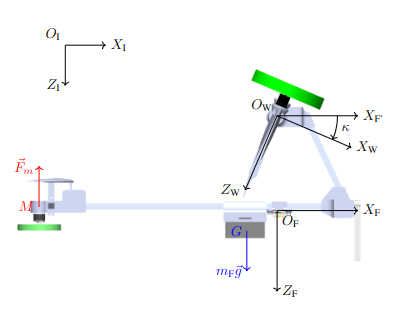
\includegraphics[width=1\columnwidth,angle=0,trim={0 0 0 0.5cm},clip]{figures/fram_side_colibri.png}
    \caption{Inertial (I), fuselage (F) and wing (W) reference frames and forces acting on the Colibri UAV.}
    \label{fig:colibri_frame_side}
\end{figure}
We will use quaternions $q = \left [ \eta ~ \epsilon^\top \right]^\top  \in {\mathbb S}^3:=\{ q\in \real^4: |q| = 1\}$ to represent the orientations of the two bodies.  The ensuing rotation matrix $R(q) \in SO(3): = \{R\in \real^{3\times 3}: \; 
 R^\top R = I, \det (R)=1\}$ is uniquely defined as 
$R(q) := I +2\eta \skewsym{\epsilon} + 2\skewsym{\epsilon}^{2} = [R_{1}~R_{2}~R_{3}]$. \\
According to Figure \ref{fig:world_body} and \ref{fig:colibri_frame_side}, define the vectors $p_{\text{F}} = \overrightarrow{O_{\text{I}} O_{\text{F}}} $, $p_{\text{W}} = \overrightarrow{O_{\text{I}} O_{\text{W}}} $, $d_{\text{FW}} = \overrightarrow{O_{\text{F}} O_{\text{W}}} $ satisfying $d_{\text{FW}} = p_{\text{W}} - p_{\text{F}}$ and $d_{\text{M}O_{\text{W}}} = \overrightarrow{\text{M} O_{\text{W}} }$, $d_{\text{G}O_{\text{W}}} = \overrightarrow{\text{G} O_{\text{W}} }$.

The overall state vector is $(x,v) \in \real^{28}$ with $x=(p_{\text{W}},~q_{\text{W}},~p_{\text{F}},~q_{\text{F}}) \in \real^{14}$ and $v=(v_{\text{W}},~\dot{q}_{\text{W}},~v_{\text{F}},~\dot{q}_{\text{F}}) = (\dot{p}_{\text{W}},~\dot{q}_{\text{W}},~\dot{p}_{\text{F}},~\dot{q}_{\text{F}})=\dot{x} \in \real^{14}$, where $v_{\text{W}} = \dot{p}_{\text{W}} \in \real^{3}$ represents the linear velocity of the wing in the inertial reference frame, $\dot{q}_{\text{W}} \in \real^{4}$ is the derivative of the quaternion, $q_{\text{W}} \in \real^{4}$ representing the orientation of the wing, $v_{\text{F}} =p_{\text{F}} \in \real^{3}$ is the linear velocity of the fuselage in the inertial reference frame and $\dot{q}_{\text{F}} \in \real^{4}$ is the derivative of the quaternion $q_{\text{F}} \in \real^{4}$ representing the fuselage orientation. It can be seen that the state vector is not minimal. It should be noted that the angular velocity $\omega \in \real^{3}$ can be obtained from the quaternion derivative $\dot{q}$ using equation  \cite[equation (2.7)]{udwadia-schutte} recalled here: 
\begin{align*}
    \omega = H(q) \dot{q} 
\end{align*}
where $H(q) \in \real^{3\times4}$ is a matrix defined by $H(q) = 2\begin{bmatrix}-\epsilon & \eta I_{3} - \skewsym{\epsilon}\end{bmatrix}$.
For deriving the equations of motion, recalling that $R_{i}(q) \in \real^{3}, i = 1,2,3$ are the three columns of a rotation matrix associated with quaternion $q$, define matrices  $L_{\text{i}}^{\text{W}} \left( q_{\text{W}} \right) = \frac{\partial R_{i}}{\partial q}(q_{\text{W}}) \in \real^{3\times4}$, 
$L_{\text{i}}^{\text{F}} \left( q_{\text{F}} \right) = \frac{\partial R_{i}}{\partial q}(q_{\text{F}}) \in \real^{3\times4}$ and
$L_{O_{\text{F}}^{\text{W}}} = \sum_{i=1}^{3} d_{\text{FW}}(i) L_{\text{i}}^{\text{F}} (q_{\text{F}})$, $i \in {1,2,3}$, where $d_{\text{FW}}(i)$ denotes the i-th component of vector $d_{\text{FW}} = p_{\text{W}} - p_{\text{F}}$. Since $O_{\text{W}}$ is located at the wing's center of rotation, the distance $d_{\text{FW}}$ is a constant, since $O_{\text{W}}$ and $O_{\text{F}}$ can be assumed to belong to the same solid (the fuselage). We deduce, with homogeneity, $\dot{L}_{O_{\text{F}}^{\text{W}}} = \sum_{i=1}^{3} d_{\text{FW}}(i) L_{\text{i}}^{\text{F}} (\dot{q}_{\text{F}})$. With these definitions, select the matrices in (\ref{eq:udwadia}) as
\begin{align}
    M = \begin{bmatrix}
        m_{\text{W}} I_{3} & \mathbb{0}_{3 \times 4} & \mathbb{0}_{3} & \mathbb{0}_{3 \times 4}\\
        \mathbb{0}_{4 \times 3} & H_{\text{W}}^\top J_{\text{W}} H_{\text{W}} & \mathbb{0}_{4 \times 3} & \mathbb{0}_{4}\\
        \mathbb{0}_{3} & \mathbb{0}_{3 \times 4} & m_{\text{F}} I_{3} & \mathbb{0}_{3 \times 4} \\
        \mathbb{0}_{4 \times 3} & \mathbb{0}_{4 } & \mathbb{0}_{4 \times 3} & H_{\text{F}}^\top J_{\text{F}} H_{\text{F}}    \end{bmatrix}\in \real^{14\times14},
\end{align}
where we denoted $H_{\text{W}} = H(q_{\text{W}})$, $H_{\text{F}} = H(q_{\text{F}})$, and
\begin{align}
    Q = \begin{bmatrix}
            m_{\text{W}} g e_3 + R(q_{\text{W}}) F_{\text{b}}\\
            -2\dot{H}_{\text{W}}^\top J_{\text{W}} \dot{H}_{\text{W}} \dot{q}_{\text{W}} + H_{\text{W}}^\top M_{\text{W}}\\
            m_{\text{F}} g e_3 + R(q_{\text{F}}) F_{\text{F}}\\
            -2\dot{H}_{\text{F}}^\top J_{\text{F}} \dot{H}_{\text{F}} \dot{q}_{\text{F}} + H_{\text{F}}^\top M_{\text{F}}\\
        \end{bmatrix} \in \real^{14},
\end{align}
% \todo{Details of forces and moments generated while the wing
% transits its position should be given in detail as this is
% the key distinct feature of this aircraft.}
where $\dot{H}_{\text{W}}$ denote $H(\dot{q}_{\text{W}})$, coinciding with the time derivative of $H(q_{\text{W}})$ and $\dot{H}_{\text{F}}$ denote $H(\dot{q}_{\text{F}})$, coinciding with the time derivative of $H(q_{\text{F}})$. Moreover, $F_{\text{b}}$ and $M_{\text{b}}$ represent, respectively,  all the forces and moments acting on the wing. The expressions of $M$ and $Q$ are taken from  \cite[equations (45) and (57)]{doi:10.2514/1.G003374} where the $\phi$ theory is developed, a parametrisation that allows the classical angles of incidence and sideslip to be subtracted and the hover singularity to be avoided. For lack of space, they will not be more detailed. Finally, $F_{\text{F}} =  F_{m}$ et $M_{\text{F}}$ represent respectively the set of non-gravitational forces and moments acting on the fuselage expressed in the frame $O_{\text{W}}$. In particular, $F_{m} = - k_{f} {u_{\text{tail}}}^{2}$ is the force generated by the motor located at the tail of the fuselage and $u_{\text{tail}}$ is the motor rotation speed, while
\begin{align}
    M_{\text{F}} =  m_{\text{F}} g e_3 \times d_{\text{G}O_{\text{W}}} + F_{m} \times d_{\text{M}O_{\text{W}}},
\end{align}
where $d_{\text{M}O_{\text{W}}}$ is the distance between the motor location and the center of rotation and $d_{\text{G}O_{\text{W}}}$ is the distance between the location of the fuselage's center of gravity and the center of rotation.

The set of constraints associated with the nonminimality or the state $(x,v)$ and by the pivot connection between the two bodies is given by:
\begin{align}
    \label{eq:contraintes}
    \left\{
    \begin{aligned}
    &\varphi_{1} \coloneqq q_{\text{W}}^\top q_{\text{W}} - 1 = 0\\
    &\varphi_{2} \coloneqq q_{\text{F}}^\top q_{\text{F}} - 1 = 0\\
    &\varphi_{3} \coloneqq R_{2}(q_{\text{W}})^\top R_{3}(q_{\text{F}}) = 0\\
    &\varphi_{4} \coloneqq R_{2}(q_{\text{W}})^\top R_{1}(q_{\text{F}}) = 0\\
    &\varphi_{5} \coloneqq p_{\text{F}} + d_{\text{FA}} + p_{\text{W}} = 0
    \end{aligned}
    \right.
\end{align}

The first two constraints impose the unit norm of the quaternions $q_{\text{F}}$ and $q_{\text{W}}$.
The third and fourth constraints are related to a moving pivot constraint, i.e. the orthogonality of two vectors is imposed. The last one is a positional constraint so that the point of the centre of rotation belonging to the wing coincides with the point defined in the fuselage. This constraint is based on a three-dimensional geometric closure.\\
It is more convenient to express the set of constraints as a stable dynamical system converging to zero, so we convert each one of the constraints in the form:
\begin{align}
    \ddot{\varphi_{i}} + \delta_{1} \dot{\varphi_{i}}  + \delta_{2} \varphi_{i} = 0, i \in {1,2,3,4,5},
\end{align}
with the selections $(\delta_{1}, \delta_{2}) = (0.5,~8)$ being the coefficients of a stable polynomial, so that, regardless of the selection $\varphi_{i}(0) = 0$, we have $\lim\limits_{t \to \infty} \varphi_{i}(t) = 0$. By differentiating constraints (\ref{eq:contraintes}) twice and factoring them out in the form $ A(x,\dot{x}) \ddot{x} = B(x,\dot{x})$, we obtain the expression of $A(x,\dot{x})$ reported in equation  (\ref{eq:A_contraint}) and $B(x,\dot{x})$ reported in the equation  (\ref{eq:b_contraint}) at the start of the next page.

\begin{align}
\label{eq:A_contraint}
    A = \begin{bmatrix}
            \mathbb{0}_{1 \times 3} & q_{\text{W}}^\top & \mathbb{0}_{1 \times 3} & \mathbb{0}_{1 \times 4}\\
            \mathbb{0}_{1 \times 3} & \mathbb{0}_{1 \times 4} & \mathbb{0}_{1 \times 3} & q_{\text{F}}^\top\\
            \mathbb{0}_{1 \times 3} & R_{3}(q_{\text{F}})^\top L_{2}^{\text{W}}( q_{\text{W}} ) & \mathbb{0}_{1 \times 3} & R_{2}(q_{\text{W}})^\top L_{3}^{\text{F}}( q_{\text{F}} ) \\
            \mathbb{0}_{1 \times 3} & R_{1}(q_{\text{F}})^\top L_{2}^{\text{W}}( q_{\text{W}} ) & \mathbb{0}_{1 \times 3} & R_{2}(q_{\text{W}})^\top L_{3}^{\text{F}}( q_{\text{F}} ) \\
            \mathbb{I}_{3} & L_{O_{\text{F}}^{\text{W}}} & -\mathbb{I}_{3} & \mathbb{0}_{3 \times 4}
        \end{bmatrix}
\end{align}

The simulation of a drone remains complex, as it is naturally unstable. We have chosen to use the control law proposed in \cite{SANSOU20221} extended to 6 DOF dynamics to stabilize the system. This PI-based control stabilises the wing. Another control law based on a proportional-derivative feedback stabilises the fuselage to keep it horizontal. The closed-loop simulation results are shown in Figure \ref{fig:sim_colibri}.
\begin{figure}[!h]
\centering
    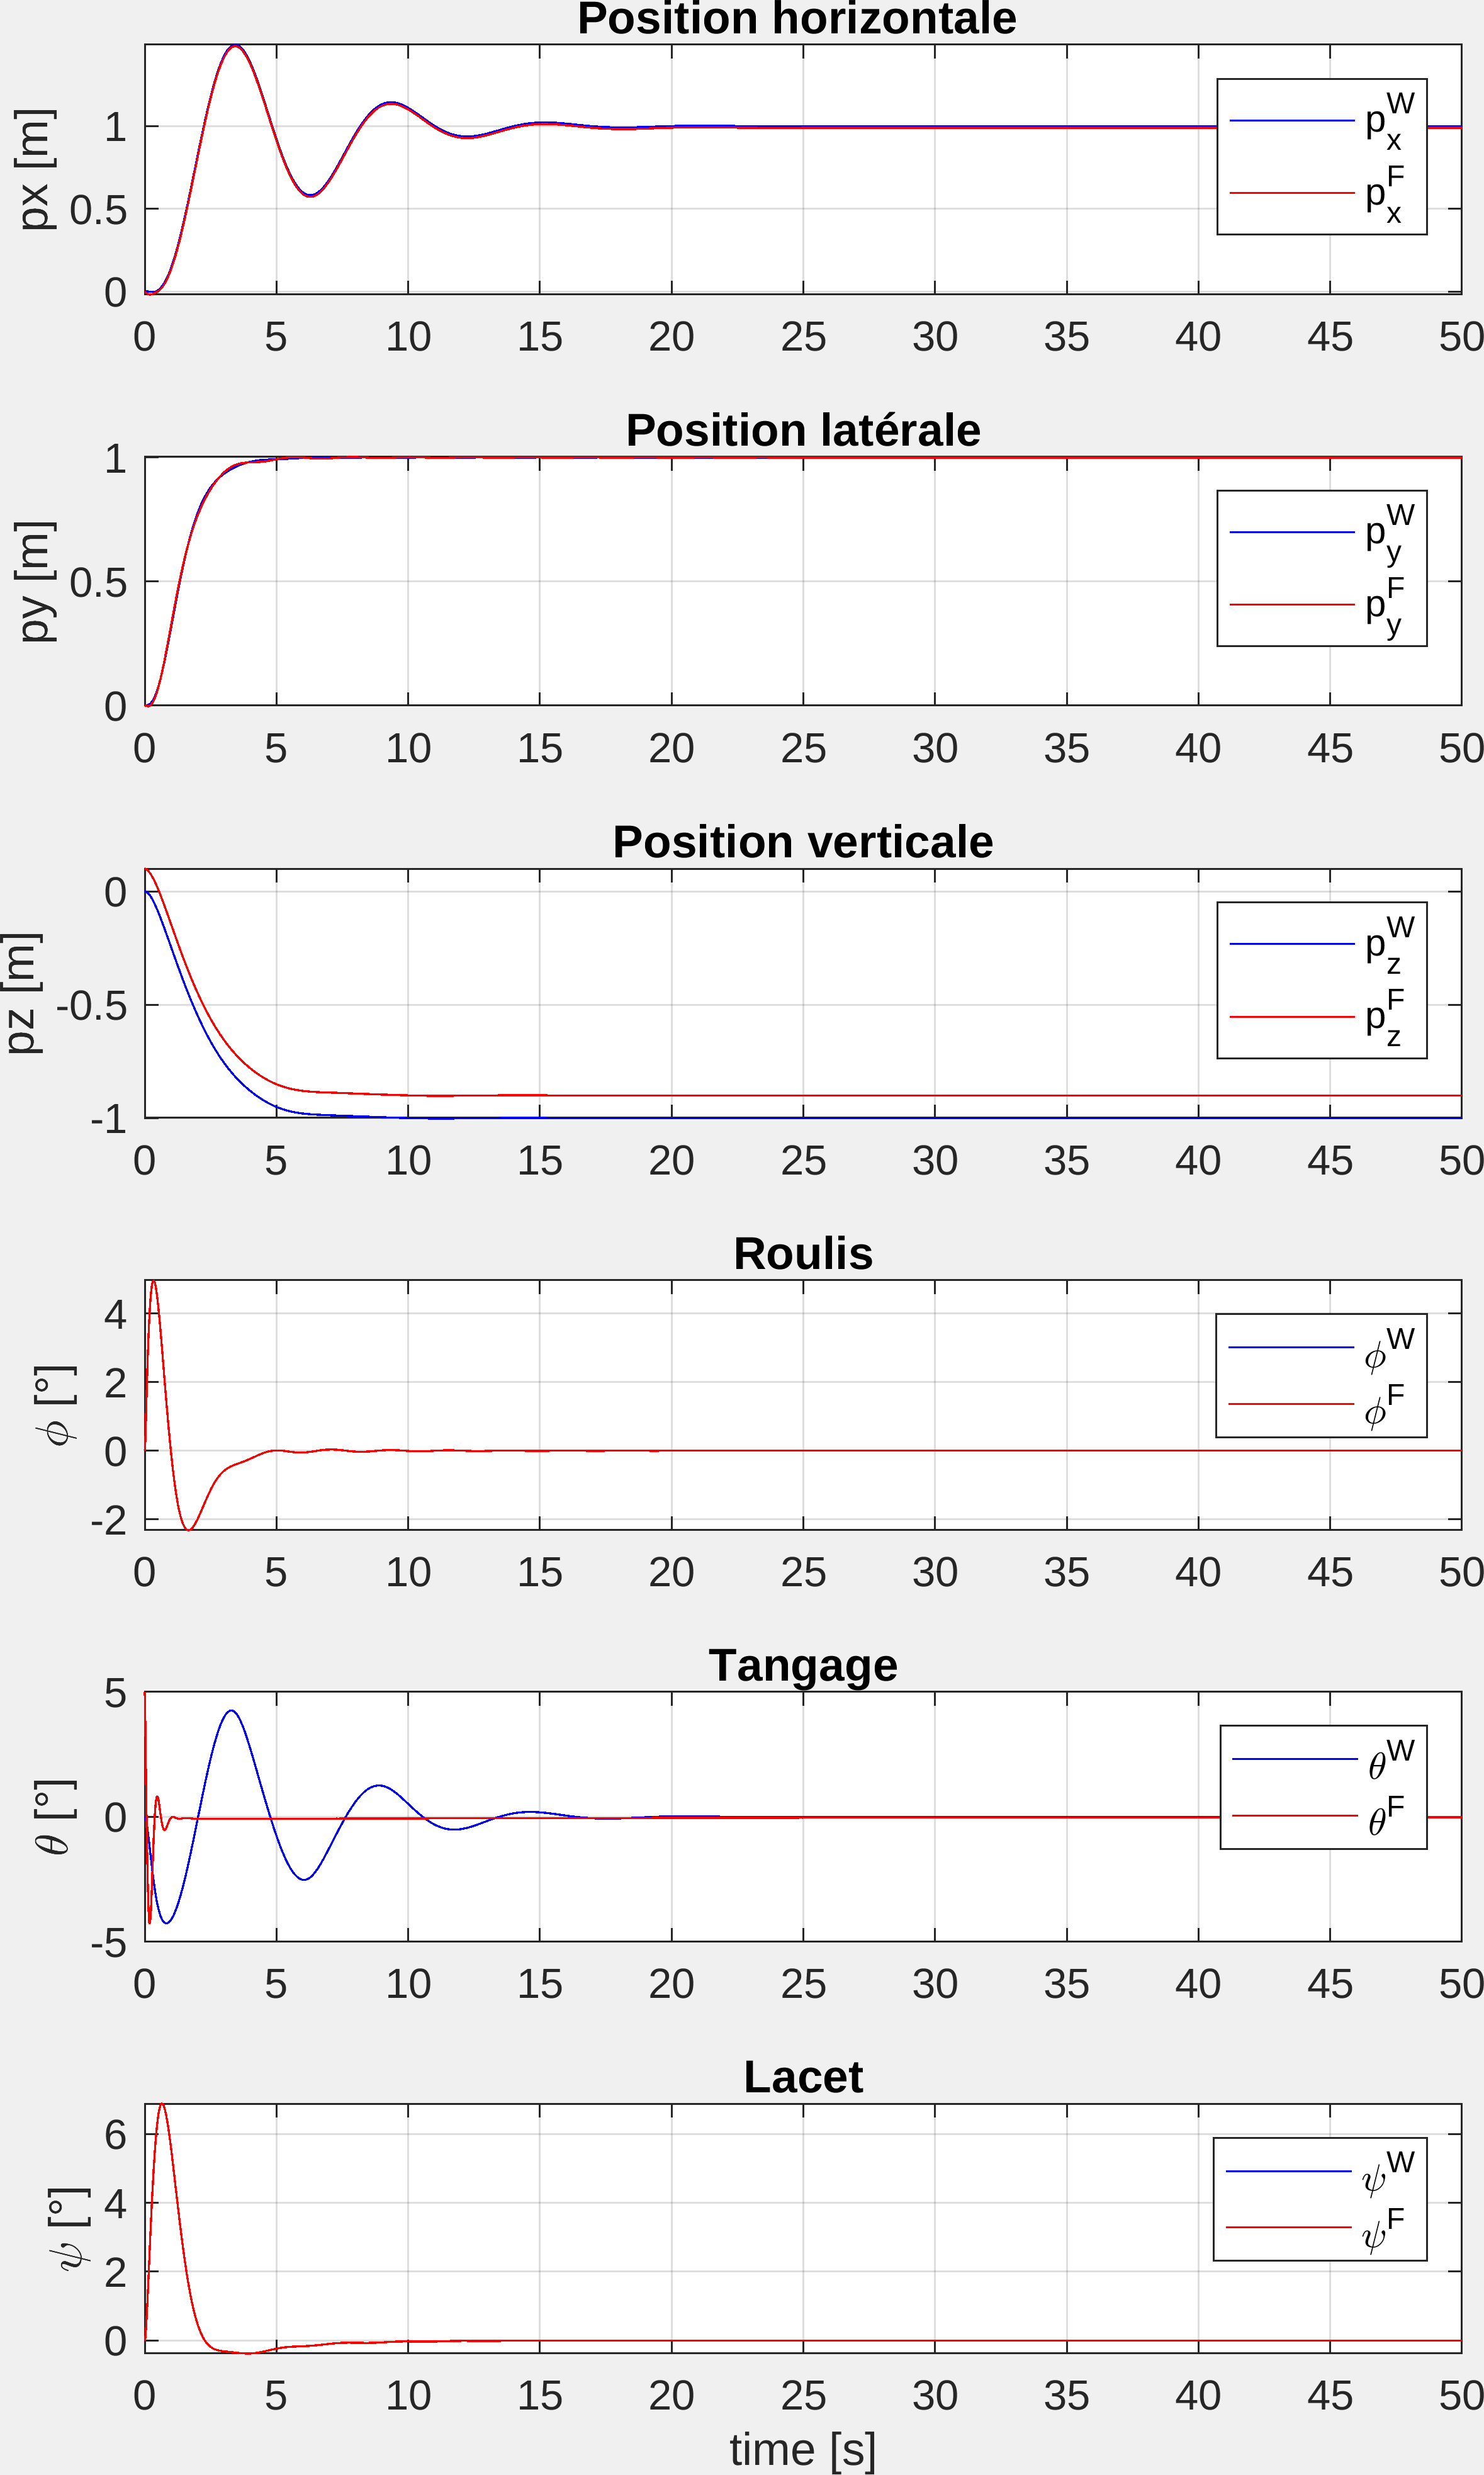
\includegraphics[width=1\columnwidth,angle=0]{figures/colibri_sim.png}
    \caption{Position and orientation simulation of the multi-body UAV Colibri in closed loop with a simple double-loop controller. }
    \label{fig:sim_colibri}
\end{figure}
Considering the degrees of freedom of the pivot link, the coupling between the two bodies is clearly visible from the lower three plots. Indeed, the roll and yaw angles $(\phi_{\text{F}}, \psi_{\text{F}})$ and $(\phi_{\text{W}}, \psi_{\text{W}})$ of the fuselage and wing coincide perfectly, while the pitch angles $(\theta{\text{F}}, \theta{\text{F}})$ are radically different.

\begin{figure*} [!h]
\begin{align}
\label{eq:b_contraint}
    B = \begin{bmatrix}
            -\delta_{1} q_{\text{W}}^\top \dot{q}_{\text{W}} - \frac{\delta_{2}}{2} (q_{\text{W}}^\top q_{\text{W}} -1) - \dot{q}_{\text{W}}^\top \dot{q}_{\text{W}} \\
            -\delta_{1} q_{\text{F}}^\top \dot{q}_{\text{F}} - \frac{\delta_{2}}{2} (q_{\text{F}}^\top q_{\text{F}} -1) - \dot{q}_{\text{F}}^\top \dot{q}_{\text{F}} \\
            -R_{3}(q_{\text{F}})^\top \dot{L}_{2}^{\text{W}}\dot{q}_{\text{W}} - R_{2}(q_{\text{W}})^\top \dot{L}_{3}^{\text{F}} \dot{q}_{\text{F}} - 2\dot{q}_{\text{W}}^\top {L_{2}^{\text{W}}}^\top L_{3}^{\text{F}} \dot{q}_{\text{F}} - \delta_{1}(R_{3}(q_{\text{F}})^\top L_{2}^{\text{W}}\dot{q}_{\text{W}} +  R_{2}(q_{\text{W}})^\top L_{3}^{\text{F}} \dot{q}_{\text{F}} ) - \delta_{2}\varphi_{3}\\
            -R_{1}(q_{\text{F}})^\top \dot{L}_{2}^{\text{W}}\dot{q}_{\text{W}} - R_{2}(q_{\text{W}})^\top \dot{L}_{1}^{\text{F}} \dot{q}_{\text{F}} - 2\dot{q}_{\text{W}}^\top {L_{2}^{\text{W}}}^\top L_{1}^{\text{F}} \dot{q}_{\text{F}} - \delta_{1}(R_{1}(q_{\text{F}})^\top L_{2}^{\text{W}}\dot{q}_{\text{W}} +  R_{2}(q_{\text{W}})^\top L_{1}^{\text{F}} \dot{q}_{\text{F}} ) - \delta_{2} \varphi_{4}\\
            \dot{L}_{O_{\text{F}}^{\text{W}}} \dot{q}_{\text{F}}  - \delta_{1}( v_{\text{W}} + \dot{L}_{O_{\text{F}}^{\text{W}}} \dot{q}_{\text{W}} - v_{\text{F}}) - \delta_{1}\varphi_{5}
        \end{bmatrix}
\end{align}
  \hrulefill\par
\end{figure*}




\section{State estimation}\label{sec:stateEst}
% \todo{Link to the modeling:  What is the connection between angular velocity
% estimation and the multibody dynamics derived in the paper?
% What are the advantages of the angular velocity estimator
% compared to existing technologies? It is difficult to
% discern the theoretical contribution to the angular
% velocity estimation part.}
In order to stabilise this two-body UAV system, it is necessary to know the position and orientation of the two bodies. Due to the pivot link between the wing and the fuselage, the difference between the orientation of the wing and the orientation of the fuselage is simply a rotation about the pitch axis of the wing. The two other orientations (roll and yaw) coincide. The position of the fuselage's centre of gravity can be deduced from the position of the wing's centre of gravity and the angle between the fuselage and the wing. This angle is measured by a quadrature rotary encoder (CUI Devices AMT22, Absolute Encoders, 12 bit, SPI), which returns a quantized angular measurement with a step size of \SI{0.09}{\degree}. Given this angular measurement, we discuss below the estimation of the speed information, so as to reconstruct the state of the UAV. 

\subsection{Sensors placement}
\label{subsec:sens_pos}
A first question pertains to the sensors placements: the IMU (accelerometer, gyroscope and magnetometer) can be installed on the fuselage or on the wing. 
Installing the IMU on the wing means that the measurements can be taken directly in the desired reference frame, but the measurements are noisier because the IMU is attached to the structure supporting the motors. Given the size of the wing, their flexibility can generate resonances and can perturb the measurements. 
%In addition, wiring the IMU is not easy as the cables must pass through the pivot link, which generates resistive torques.
Installing the IMU on the fuselage reduces vibrations, but means that the measurements must be transformed in the wing reference frame. The corresponding transformation can be computed from the rotary encoder measurement, providing the angle between the wing and the fuselage, and also from the measurements taken with the CAD software, providing precise information about the distances between the wing and fuselage frames. Our final choice is to attach the IMU to the fuselage. Another consideration is that the autopilot board, which already have an integrated IMU, is also supposed to be connected to the payload and other sensors attached to the fuselage. It is thus limiting the number of cables at the pivot point to the actuators commands and power supply.

\subsection{Angular speed estimation}
As explained above, we can measure the angle $\kappa \in \real$ between the wing and the fuselage using the rotary encoder. Then, to estimate the angular velocity we use the high-gain observer proposed in \cite{203613} (see also \cite{1032320} for the use of high-gain observers to estimate time derivatives). This method is preferable to a finite difference derivative, as the quantized information generated by the rotary encoder can result in bursts in the estimated angular velocity values.\\ 
Denote by $\kappa \in \real$ the measured position variable, by $\omega_{\kappa} := \dot \kappa  \in \real$ its derivative, to be estimated, and by $\xi = [\kappa,~\omega_{\kappa}]^\top \in \mathbb{R}^2$ their juxtaposition in a single vector. Denote also $\hat{\xi}$ the estimate of $\xi$ as follows:
%\todo{GH: il y a pas un peu de répétitions dans les notations ?}
%\xi = [\kappa,~\omega_{\kappa}]^\top \in \mathbb{R}^2, \quad 
\begin{align*}
    \hat{\xi} = [\hat{\kappa},~\hat{\omega}_{\kappa}]^\top \in \mathbb{R}^2.
\end{align*}
Following \cite{203613}, the estimator dynamics is given by
\begin{align}
\label{eq:high_dyn}
    \dot{\hat{\xi}} =  \begin{bmatrix}0 & 1 \\ 0 & 0 \end{bmatrix} \hat{\xi}+ \begin{bmatrix}\frac{k_{p}}{\epsilon_{\kappa}}  \\ \frac{k_{v}}{\epsilon_{\kappa}^{2}}  \end{bmatrix} (\kappa - \hat{\kappa}),
\end{align}
where $\kappa$ is the angular measurement recovering from the sensors, $k_{p}$ and $k_{v}$ are two positive scalars gains such that the characteristic equation $s^{2} + k_{v} s + k_{p} = 0$ has roots with negative real part. For our estimators, we have selected $k_{p} = 1$ and $k_{v} = 1.3$ so as to get a damping factor $\zeta = 0.65$ leading to a slightly underdamped response as a suitable trade-off between a fast rise time and a mildly oscillatory response. The high-gain scaling factor
$\epsilon_{\kappa}$ can be conveniently adjusted in order to obtain a trade-off between smoothing action (obtained by increasing $\epsilon_{\kappa}$) and reduction of the time lag
of the estimator (obtained by reducing $\epsilon_{\kappa}$). Moreover, the smoothing action of the proposed approach mitigates the effect of the quantized position measurements. We have selected $\epsilon_{\kappa} = 0.05$ for our experiments. Figure \ref{fig:high_gain} shows the experimental results obtained after implementation of the high-gain filter (\ref{eq:high_dyn}) in the case of a flight generating high-amplitude angular oscillations.
\begin{figure}[h]
\centering
    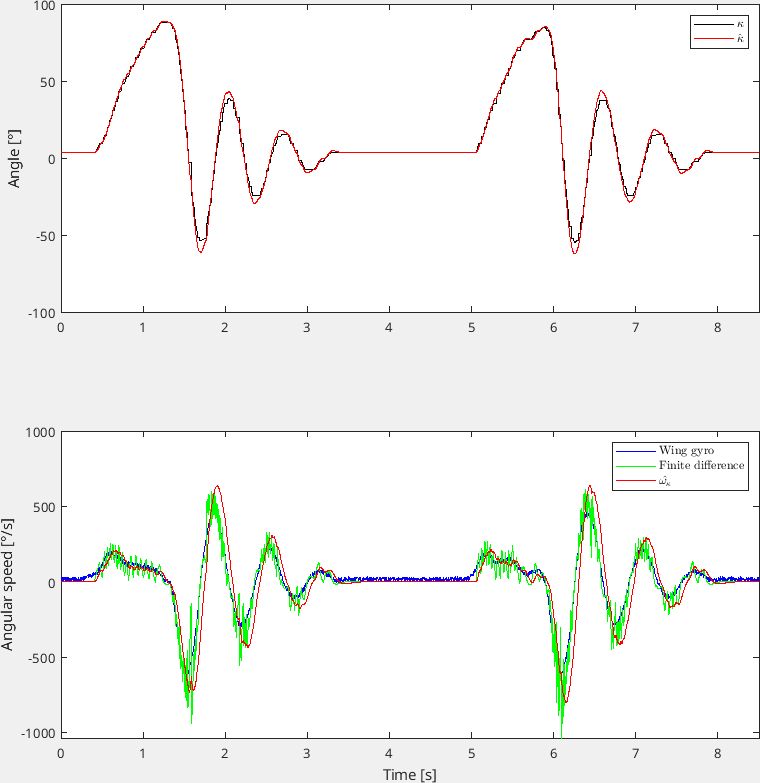
\includegraphics[width=1\columnwidth,angle=0]{figures/highGainFilter.png}
    \caption{Angular position measurement (black,top plot), wing gyro velocity measurement (blue,bottom plot), finite difference velocity estimation (green, bottom plot) and high-gain estimates (red curves)}
    \label{fig:high_gain}
\end{figure}
%\todo{GH: c'est pas très lisible comme figure}
We carried out differentiation by finite difference (in green) in post-treatment to compare the results. Due to the quantized nature of the rotary encoder, we observe that the angular velocity obtained by finite difference is very noisy. We can see that the high-gain filter makes it possible to estimate the angular velocity more accurately (in red), albeit with a slight delay. Thanks to the addition of an extra IMU on the wing in a specific flight test, it is possible to compare the velocity estimate with the wing's gyroscope (MPU9250) measurements, visible on the bottom graph of Figure \ref{fig:high_gain} (blue trace). We can see that the gyroscope readings are somewhat noisy, due in particular to the vibrations generated by the motors.  %\todo{GH: ref à la figure est trop tard par rapport au texte}
\\
In order to perform the necessary transformation among the reference frames, define the quaternion $q_{\hat{\kappa}} \in {\mathbb S}^3$ as follows:
\begin{align}
\label{eq:rot_quat}
    q_{\hat{\kappa}} =  \left [\cos\left(\frac{\hat{\kappa}}{2}\right) ~ 0 ~ \sin\left(\frac{\hat{\kappa}}{2}\right) ~ 0 \right]^\top
\end{align}


\subsection{Wing state estimation}
Based on the estimated angle $\hat{\kappa}$ and the estimated angular velocity $\hat{\omega}_{\kappa}$, it is possible to transform the measurements from the fuselage to the wing frame. All the sensors are installed on the autopilot board, which is itself attached to the fuselage. However, as mention in introduction, we want to use INDI to stabilize the wing. So this control law requires the state information in the wing reference frame, where all the forces are applied (aerodynamic and traction).
Then, two viable solution are possible: perform the state estimation in the fuselage reference frame and rotate the estimation, using the estimate of the angle $\hat{\kappa}$, or rotate the raw measurements in advance to express them in the wing reference frame, and then perform the state estimation on the latter. 
Given the current architecture of the software in the Paparazzi\footnote{\url{https://github.com/enacuavlab/paparazzi/tree/rot_state_est}} system, it is cumbersome to have two joint state estimation structures, so it is difficult to implement the first solution, where the controller directly retrieves the current state estimation. For this reason, we have chosen to estimate the state of the wing from data measured on the fuselage. To this end, we detail below the coordinate transformation for the three sensors: gyroscope, accelerometer and magnetometer. \\
\indent For the gyroscope-based angular rate measurements, we may compute the angular velocity of the wing expressed in the wing frame as
\begin{align}
    \label{eq:gyro_deplacement}
    \omega_{\text{W}} = R(q_{\hat{\kappa}}) \left( \omega_{gyro}^{\text{F}} + \begin{bmatrix}
    0\\ \omega_{\kappa} \\ 0
    \end{bmatrix}  \right) 
\end{align}
where $\omega_{gyro}^{\text{F}}$ is the angular velocity measured by the gyro on the fuselage, expressed in the fuselage frame, $\hat{\omega}_{\kappa}$ is the estimated angular velocity of the wing relative to the fuselage, as per (\ref{eq:high_dyn}), and $q_{\hat{\kappa}}$ is the quaternion defined in (\ref{eq:rot_quat}).
Expression (\ref{eq:gyro_deplacement}) is similar to a composition of angular velocities and a reference frame transformation.\\
\indent For the acceleration measurement with the accelerometer, we may use the following relation
Expression (\ref{eq:accel_deplacement}) is obtained from the rate of change transport theorem \cite{brizard2004motion}, where we find the Euler acceleration term $\dot{\omega_{\text{F}}} \times d_{AF}$ and the centripetal acceleration term $\omega_{\text{F}} \times ( \omega_{\text{F}} \times  d_{AF})$. Coriolis Acceleration $2\omega_{\text{F}} \times \frac{d (d_{\text{FW}})}{d t}\Bigr|_{O_{\text{F}}}$ and the rate of acceleration $\frac{d^{2} (d_{\text{FW}})}{d^{2} t}\Bigr|_{O_{\text{F}}}$ are zero because $d_{\text{FW}}$ is contant.
\begin{align}
    \label{eq:accel_deplacement}
    a_{\text{W}} = R(q_{\hat{\kappa}}) \left( a_{acc}^{F} + \dot{\omega}_{gyro}^{F} \times d_{\text{FW}} + \omega_{gyro}^{F} \times ( \omega_{gyro}^{F} \times  d_{\text{FW}}) \right) 
\end{align}
where $a_{acc}^{F} \in \real^{3}$ is the acceleration measured by the accelerometer on the fuselage, expressed in the fuselage frame and $\omega_{gyro}^{F}$, the angular velocity of the fuselage, same as the equation (\ref{eq:gyro_deplacement}). The angular acceleration $\dot{\omega}_{gyro}^{F}$ in (\ref{eq:accel_deplacement}) is computed by a finite difference.\\
\indent For the magnetometer measurements, we have
\begin{align}
    \label{eq:mag_deplacement}
    E_{\text{W}} = R(q_{\hat{\kappa}}) E_{mag}
\end{align}
where $E_{mag} \in \real^{3}$ is the magnetometer output, expressed in the fuselage frame and  $ E_{\text{W}} \in \real^{3}$ is the computed measurement expressed in the wing frame.\\
\indent To obtain the wing state estimate, we use a sensor measurement fusion algorithm: extended Kalman filter\footnote{\url{https://github.com/PX4/PX4-ECL/tree/master}} (EKF) which provide an estimate of the following states: $p_{\text{W}}$, $v_{\text{W}}$, $q_{\text{W}}$ from measurements transformed in the wing reference frame $\omega_{\text{W}}$ (eq. (\ref{eq:gyro_deplacement})), $a_{\text{W}}$ (eq. (\ref{eq:accel_deplacement})), $E_{\text{W}}$ (eq. (\ref{eq:mag_deplacement})) and external vision system pose data, which provides a precise measurement of the drone's position $p_{\text{W}}$ and speed $v_{\text{W}}$ in the inertial reference frame (I).

\subsection{Fuselage orientation estimation}
To determine the orientation of the fuselage, we may perform a composition between the quaternion representing the orientation of the wing $q_{\text{W}}$ result of EKF and the quaternion constructed from the filtered measurement of the rotary encoder $q_{\hat{\kappa}}$ in (\ref{eq:rot_quat}),
\begin{align}
\label{eq:quat_fuselage}
    q_{\text{F}} = q_{\text{W}} \otimes q_{\hat{\kappa}}
\end{align}
where the operator $\otimes$ denotes the qaternion product. The knowledge of $q_{\text{F}}$ is needed to keep the fuselage perfectly horizontal. 










% LTeX: language=fr enabled=true

\chapter{Modèle, commande et expérimentation d'un \textit{freewing}}
\minitoc
\label{chap:colibri}



\section{Motivation}
\label{sec:motivationcolibri}
Les nombreux avantages d'une architecture \textit{tailsitter} nous ont poussé à nous intéresser à leur stabilisation. Nous avons toutefois observé une limitation dans leur usage. Effectivement, l'aile change d'incidence en fonction de la vitesse du drone ou du vent environnent et toute charge utile se trouve en rotation avec l'aile. Ce comportement est inapproprié pour une caméra ou une sonde Pitot, lesquelles doivent pouvoir maintenir une direction constante. Ainsi, nous avons pensé à une nouvelle architecture, à mi-chemin entre un \textit{tailsitter} et un \textit{tiltwing}, appelée \textit{freewing}. Cette dernière conserve les avantages du \textit{tiltwing} en ce qu'elle permet d'avoir un fuselage que l'on peut maintenir constamment horizontal. Elle s'inspire des \textit{tailsitters} en permettant de modifier librement l'incidence de l'aile pour se désensibiliser des turbulences. L'aile étant libre de s'orienter vis-à-vis du fuselage, une augmentation de portance engendrée par une augmentation de la vitesse du flux d'air (turbulences), modifiera l'angle d'incidence de l'aile ce qui entraînera une diminution de la portance et donc un nouvel équilibre.

De plus, le fuselage permettra l'emport d'une charge utile fragile (car elle pourra être maintenue horizontale en toutes circonstances), mais aussi de capteurs et de la batterie. L'ensemble de la masse du drone sera concentré sur le fuselage de manière à minimiser l'inertie de l'aile et à faciliter sa rotation face à des turbulences faibles.

\section{Réflexion autour de diverses architectures}
{\color{blue}
La maquette utilisée dans le chapitre \ref{chap:3DOF} nous a permis d'expérimenter le comportement de l'aile en fonction de la position du centre de rotation.

Nous avons réalisé un montage permettant de modifier la position du centre de rotation par rapport au centre de gravité (figure \ref{fig:MontageDarkoReglable}). Cela impacte la stabilité de l'aile, mais aussi son comportement face au vent. 

\begin{figure}[ht!]
    \centering
   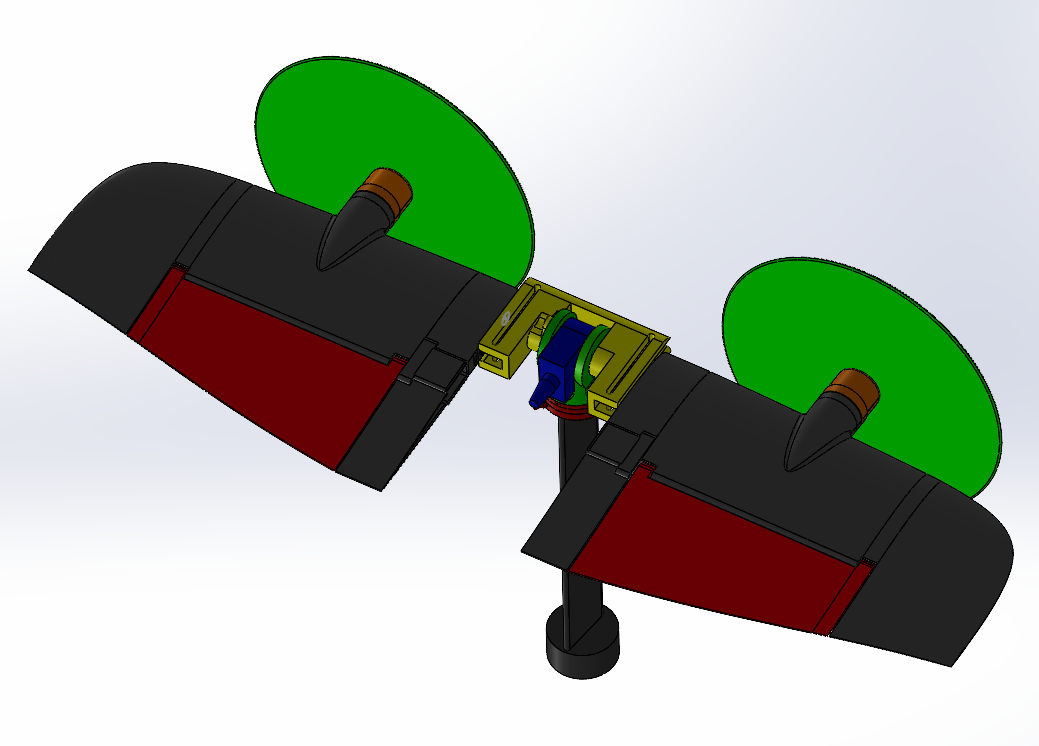
\includegraphics[width=0.7\columnwidth]{figures/vueMaquetteDarkoReglage.png}
    \caption{Montage de la maquette du chapitre \ref{chap:3DOF} avec un réglage de la position du centre de rotation (pièce jaune).}
    \label{fig:MontageDarkoReglable}
\end{figure}

La pièce jaune de la Figure \ref{fig:MontageDarkoReglable} assure la liaison entre les demi-ailes (droite et gauche) et le système de rotation central. De plus, la pièce est conçue pour permettre un glissement dans le plan des ailes, ce qui a pour conséquence de déplacer le centre de gravité de l'ensemble par rapport au centre de rotation, ce dernier étant bloqué. Nous observons sur la Figure \ref{fig:MontageDarkoReglableAvArr} que le réglage permet un débattement d'environ \SI{30}{\milli\meter}. Le montage est verrouillé par deux vis par aile, assurant la rigidité.

Le centre de gravité doit se trouver en arrière du centre de rotation pour assurer que l'aile soit verticale sans commande.

De ce montage et en utilisant la loi de stabilisation de la Figure \ref{fig:commande_int3DOF}, nous avons observé l'intérêt de positionner un fuselage pendulaire fixé en rotation libre. Ainsi l'aile se trouve libre de tourner autour de l'axe de liaison pour obtenir l'incidence nécessaire à la stabilisation du drone dans la phase de vol considérée. Nous avons choisi d'expérimenter le cas où la charge utile, ainsi que la batterie, se situent sur le fuselage de manière à diminuer l'inertie de l'aile : cela permet d'augmenter sa réactivité. Ainsi, la maquette de la Figure \ref{fig:MontageDarkoReglable} était alimentée par une batterie au plomb installée au sol avec des câbles alimentant le système installé au niveau de la fixation. Ces câbles génèrent un moment résistant, permettant d'approcher au mieux le système réel.

\begin{figure}[ht!]
    \centering
    \resizebox{.7\textwidth}{!}{%
    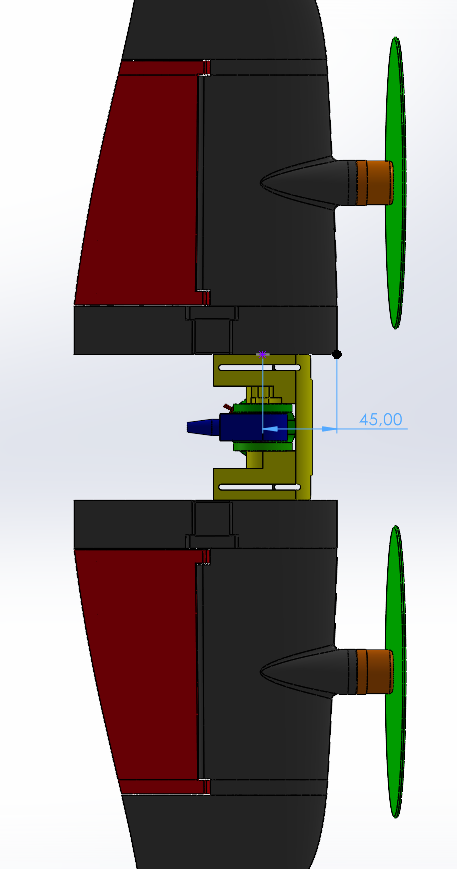
\includegraphics[height=3cm]{figures/CentreRotationAv.png}
    \quad
    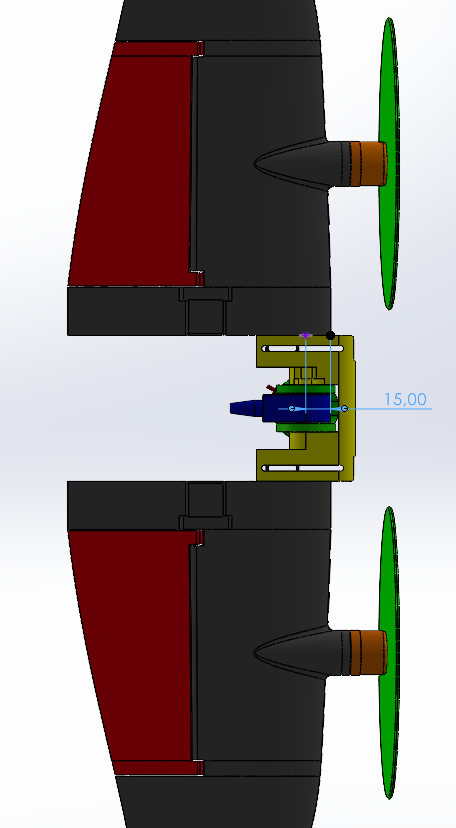
\includegraphics[height=3cm]{figures/CentreRotationArr.png}
    }
    \caption{Positionnement avant et arrière du centre de rotation par rapport au centre de gravité.}
    \label{fig:MontageDarkoReglableAvArr}
\end{figure}

Au niveau de l'actionnement, le parti pris a été d'utiliser un mécanisme similaire à celui de DarkO, étant donné les études préliminaires réalisées sur la modélisation, l'étude des couplages et des saturations. Toutefois, il existait d'autres possibilités.

Nous pouvions monter les moteurs sur des nacelles pour supprimer les élevons et générer de la poussée vectorielle. Ce mécanisme ne supprime aucun actionneur car le servomoteur présent sur l'élevon se retrouve à actionner la nacelle. Ce servomoteur doit être dimensionné pour vaincre les effets gyroscopiques de l'hélice, ce qui peut diminuer la réactivité de l'actionnement. De plus, le mécanisme de nacelle augmente le nombre de pièces en mouvement, ce qui pose des problèmes de fiabilité. L'absence de commande aérodynamique ne permet pas de vol plané en cas de panne moteur, donc le contrôle du drone ne peut pas être assuré.

Une autre possibilité était de motoriser l'intégralité d'une demi-aile, ce qui permettrait de modifier la direction de poussée de moteur, mais aussi de modifier l'incidence de l'aile. Toutefois, vu les dimensions de l'aile, les servomoteurs doivent être dimensionnés au vu des effets gyroscopiques des hélices couplés à l'inertie de la demi aile. Cela aurait induit des servomoteurs puissants qui auraient alourdi la structure.

 Nous avons aussi évalué la possibilité de rendre les deux ailes droite et gauche indépendantes, ce qui ajoute un degré de liberté dans la dynamique du drone. Ce fonctionnement permet de se soustraire de l'impact d'une différence de vitesse air sur chacune des demi-ailes. Toutefois, il est nécessaire de mesurer l'orientation de chacune des demi-ailes, ce qui nécessite un capteur en plus dans un espace assez contraint.

 {
    \color{green}
    Bien que nous ayons convergé vers une architecture d'actionnement proche de celle de DarkO, nous avons réalisé une maquette avec une installation des moteurs en H (voir Figure \ref{fig:ColibriH}). 
    
    \begin{figure}[ht!]
        \centering
       \includegraphics[width=0.7\columnwidth]{figures/colibriH.png}
        \caption{Maquette de Colibri avec un montage des moteurs en H.}
        \label{fig:ColibriH}
    \end{figure}
    Cette architecture permet d'utiliser un différentiel moteur entre ceux placer sous l'aile et ceux sur l'aile pour contrôler le moment de tangage du drone. Le principal intérêt de cela est la suppression de la nécessité d'utiliser les élevons lors de la transition. Les élevons sont utilisés uniquement lors de vol plané.
    Effectivement, l'installation des moteurs permet d'avoir un contrôle total de la voilure (de manière similaire à un quadrirotor). Un angle a été ajouter lors de l'installation de moteur pour augmenter l'efficacité sur la rotation autour de l'axe vertical en stationnaire.
    Nous n'avons pas poursuivi dans cette direction au profit de l'architecture linaire plus aligné dans nos précédents travaux.
 }

}


\section{Design et modélisation d'un drone : Colibri}
\label{sec:model_colibri}

\subsection{Description de l'architecture}
Le drone Colibri est dérivé d'un drone \textit{tailsitter} qui génère de la portance pendant le vol d'avancement. Cette aile possède plusieurs actionneurs : quatre moteurs $u_{i}, ~i = 1,2,3,4$ et deux élevons $\delta_{\text{l}}$ et $\delta_{\text{r}}$. Nous pouvons définir le vecteur de contrôle $\boldsymbol{u}_{\text{W}}$ de l'aile d'après la Figure~\ref{fig:world_body} comme :
\begin{align}
    \label{eq:uw}
    \boldsymbol{u}_{\text{W}} = [u_{1}~u_{2}~u_{3}~u_{4}~\delta_{\text{l}}~\delta_{\text{r}}]^\top.
\end{align} Un fuselage relié par un pivot est fixé au centre aérodynamique de l'aile. Ce fuselage supporte l'autopilote, la batterie, un moteur et un empennage pour le maintenir horizontal.

Dans la Figure~\ref{fig:world_body}, toutes les surfaces de contrôle aérodynamiques sont représentées en rose et les hélices en vert. Trois repères sont attachés au drone tel que : (I) est un repère inertiel NED lié à la surface de la terre, (W) est un repère attaché à l'aile du drone et (F) est un repère attaché au fuselage du drone.



\begin{figure}[ht!]
\centering
    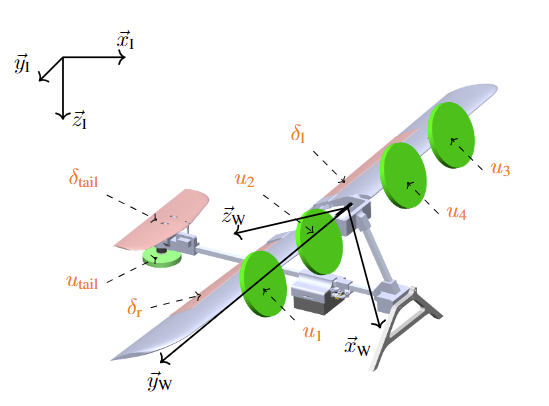
\includegraphics[width=0.6\columnwidth,angle=0,trim={0 0 0 0.5cm},clip]{figures/wold_body.png}
    \caption{Les repères, inertiel (I) et aile (W), attachés à l'architecture de Colibri.}
    \label{fig:world_body}
\end{figure}

Certaines des dimensions caractéristiques sont indiquées dans la Table~\ref{tab:pars_colibri}. Notons que les moteurs sont positionnés symétriquement sur l'aile, ce qui signifie que la position peut être décrite en se concentrant sur un seul côté. 

\begin{table}[ht]
  \centering
    \begin{tabular}{|l|c|c|}
      \hline
      \multicolumn{1}{|c|}{Paramètres} & Valeurs & Unités  \\
      \hline
      $m_{\text{W}}$ (masse de l'aile)  & 0.53& \SI{}{\kilogram} \\
      \hline
      $m_{\text{F}}$ (masse du fuselage)  & 1.17& \SI{}{\kilogram} \\
      \hline
    %   $b$ (wingspan)  & 1.17 & \SI{}{\meter} \\
    %   \hline
    %   $c$ (aerodynamic cord)  & 0.150 & \SI{}{\meter} \\
    %   \hline
    %   $S$ (wing area) & 0.1537 & \SI{}{\square\meter}\\
    %   \hline
    %   $S_{\text{wet}}$ (wet area) & 0.0813 & \SI{}{\square\meter}\\
    %   \hline
    %   $S_{\text{p}}$ (propeller area) & 0.0182 & \SI{}{\square\meter}\\
    %   \hline
      $\boldsymbol{J}_{\text{W}}=diag(J_{x}^{\text{W}}, J_{y}^{\text{W}}, J_{z}^{\text{W}})$ & \!\! $\diag(0.1677,0.0052,0.1634)$\!\! & \SI{}{\kilogram\square\meter}\\
      \hline
      $\boldsymbol{J}_{\text{F}}=diag(J_{x}^{\text{F}}, J_{y}^{\text{F}}, J_{z}^{\text{F}})$ & \!\! $\diag(0.0191,0.0161,0.0343)$\!\! & \SI{}{\kilogram\square\meter}\\
      \hline
      $k_{\text{p}}$ (coefficient hélice fuselage) & 5.13e-6 & \SI{}{\kilogram\meter}\\
      \hline
      $k_{\text{f}}$ (coefficient de poussée des hélices) & 5.13e-6 & \SI{}{\kilogram\meter}\\
      \hline
      $k_{\text{m}}$ (coefficient de moment des hélices) & 2.640e-7 & \SI{}{\kilogram\square\meter}\\
      \hline
      $\xi_{\text{f}}$ (génération de force élevon) & 0.48 & --\\
      \hline
      $\xi_{\text{m}}$ (Génération de moment élevon) & 0.93 & --\\
      \hline
       $\boldsymbol{d}_{\text{M}O_{\text{W}}}$  & $[0.383,0,-0.167]^\top$ & \SI{}{\meter}\\
      \hline
       $\boldsymbol{d}_{\text{G}O_{\text{W}}}$  & $[0.052,0,-0.171]^\top$ & \SI{}{\meter}\\
      \hline
    \end{tabular}
    \caption{Paramètres numériques du modèle Colibri.}
    \label{tab:pars_colibri}
\end{table}

{\color{blue}
    Nous avons déjà conçu un système de rotation libre dans le chapitre \ref{sec:motivation3DOF}, toutefois il était fixé à un banc de test. Pour Colibri, il est nécessaire de concevoir une liaison robuste, mais légère pour être embarquée sur le drone. 

    Nous avons donc conçu un système de rotation basé sur deux roulements à aiguille (en violet sur l'image \ref{fig:ColibriRot}) et deux butées à billes F6-12M pour minimiser le couple résistant (en jaune sur l'image \ref{fig:ColibriRot}). Les butées à  billes sont bloquées par des pièces de verrouillage (en bleu sur l'image \ref{fig:ColibriRot}) obtenues par impression 3D stéréolithographique (SLA). Ces verrouilleurs pincent le tube en carbone pour éviter qu'il coulisse de droite à gauche. 

    L'impression 3D SLA est un procédé de photopolymérisation qui utilise un laser UV pour polymériser une résine liquide en plastique durci. Cette technologie permet d'obtenir des pièces d'une grande précision et plus résistantes que l'impression 3D à dépôt de fil fondu (FDM).

    

    \nomenclature[]{\(SLA\)}{Impression 3D stéréolithographique (\textit{StereoLithography Apparatus})} 

    \nomenclature[]{\(FDM\)}{Impression 3D dépôt de fil fondu (\textit{Fused deposition modeling})} 

    \begin{figure}[ht!]
        \centering
        \resizebox{.9\textwidth}{!}{%
        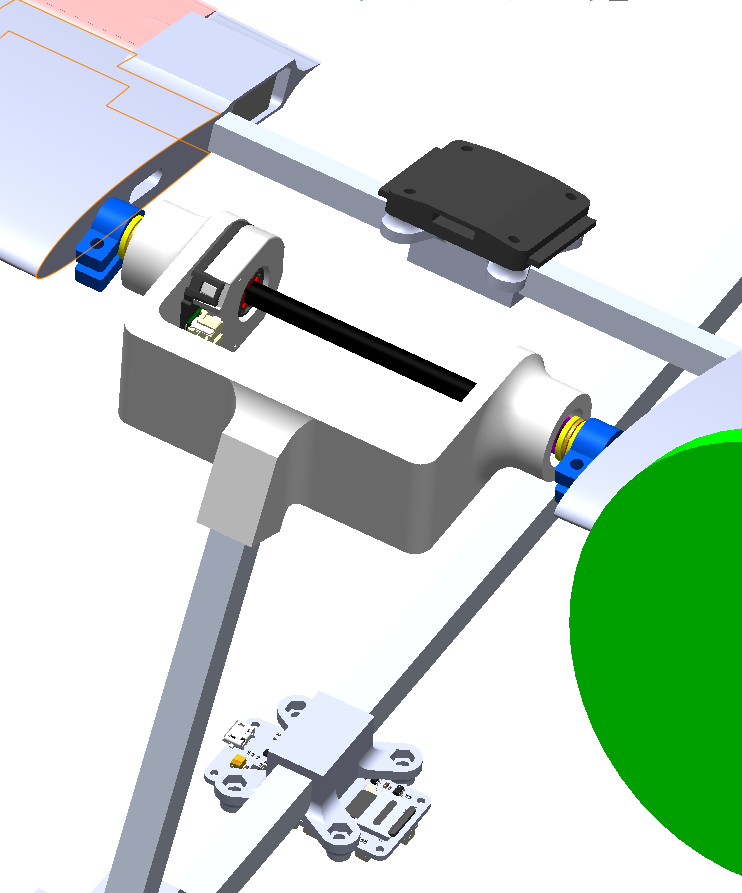
\includegraphics[height=3cm]{figures/ColibriRotPlein.png}
        \quad
        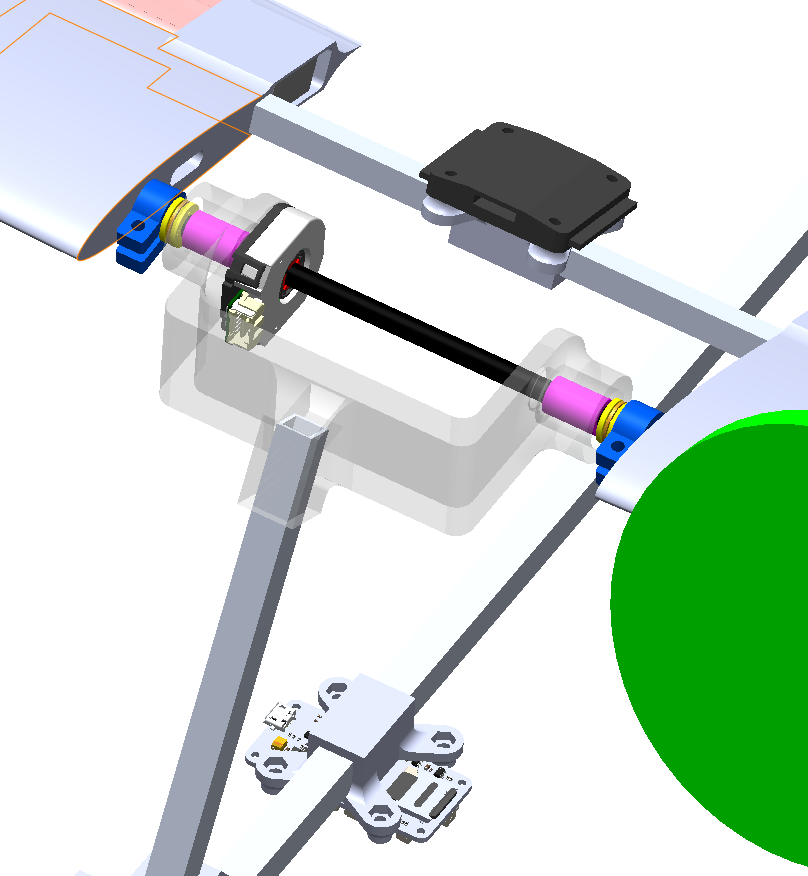
\includegraphics[height=3cm]{figures/ColibriRotTransparent.png}
        }
        \caption{Modèle 3D de la liaison.}
        \label{fig:ColibriRot}
    \end{figure}

    L'encodeur rotatif, CUI Devices AMT22 est fixé au bâti qui maintient les roulements (figure \ref{fig:ColibriRotReel} gauche). Un système de pince est installé sur le tube en carbone et permet au capteur de mesurer l'angle de rotation de l'ensemble aile par rapport au fuselage.

    \begin{figure}[ht!]
        \centering
        \resizebox{.9\textwidth}{!}{%
        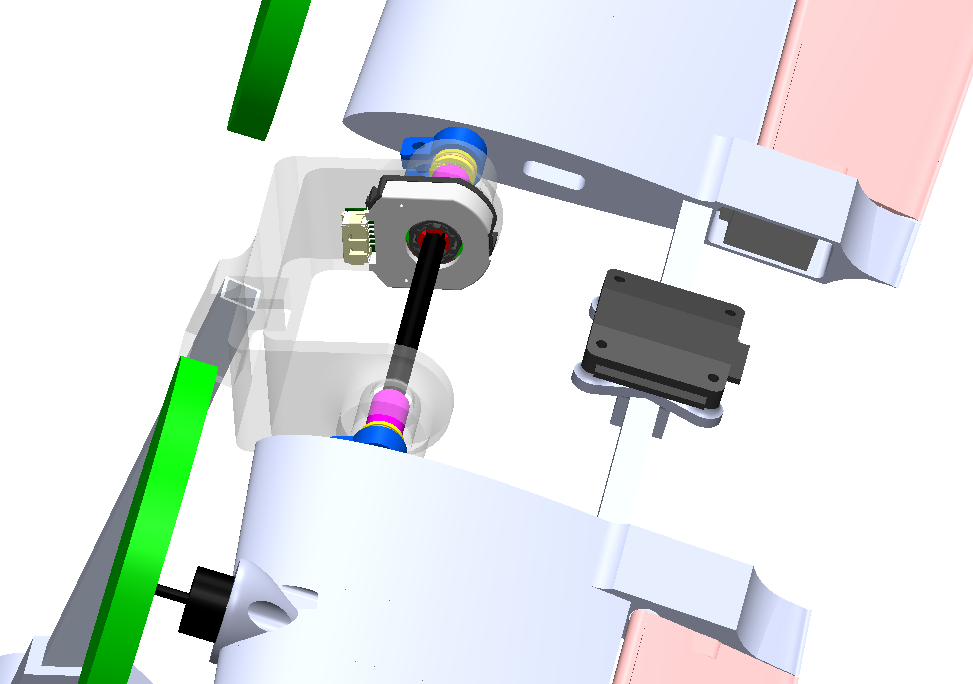
\includegraphics[height=3cm]{figures/ColibriRotVueCote.png}
        \quad
        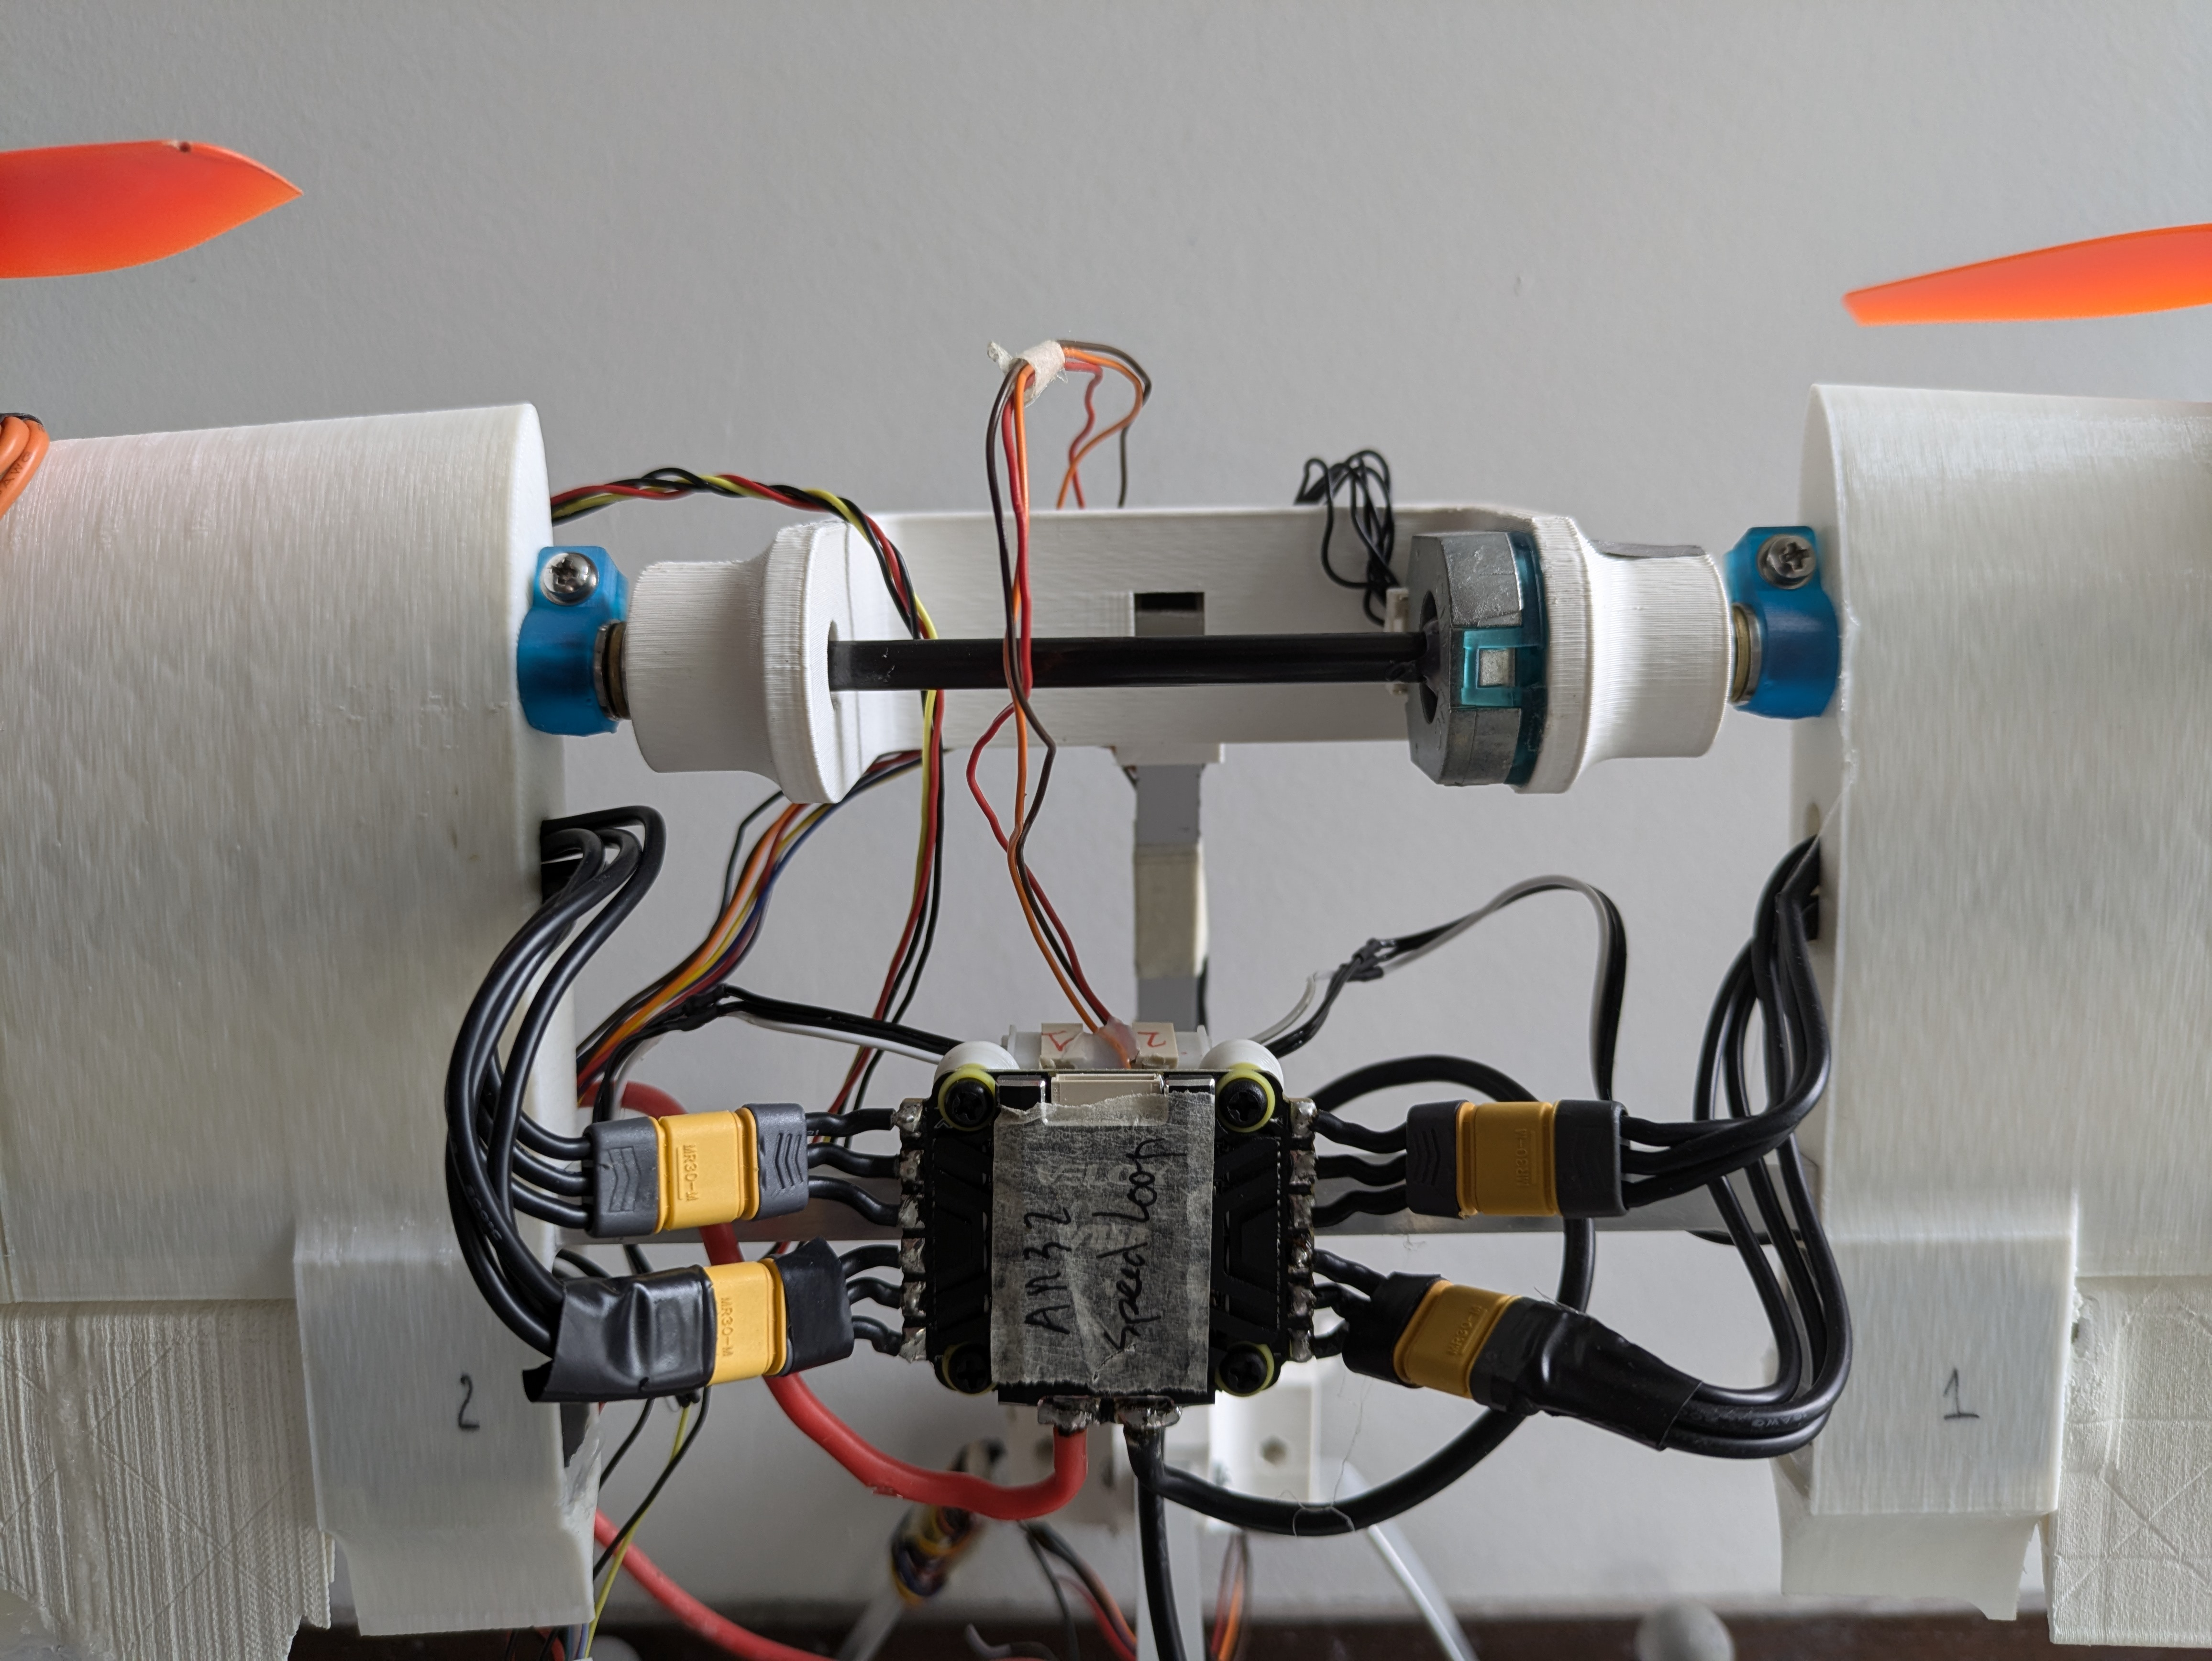
\includegraphics[height=3cm]{figures/ColibriRotReel.jpg}
        }
        \caption{Visualisation de l'encodeur rotatif sur le modèle 3D (gauche) et modèle réel (droite).}
        \label{fig:ColibriRotReel}
    \end{figure}
    Le montage réel est proposé sur la Figure \ref{fig:ColibriRotReel} de droite. Nous observons le montage du contrôleur moteur avec les fils qui vont jusqu'au moteur (3 par moteur soit un total de 12 fils) et les câbles de commande de l'ESC, les câbles de l'encodeur rotatif et les câbles de commandes des servomoteurs (3 fils, car les servomoteurs sont chainés) et enfin les câbles de l'IMU installée sur l'aile.
}

\subsection{Modélisation}
La modélisation est basée sur les résultats de \cite[Équation (2.15)]{udwadia-phohomsiri}. 
Elle est obtenue à partir de l'équation de Lagrange décrivant le mouvement d'un système à chaque instant $t$ :
\begin{align}
    \label{eq:unconstraintDyn}
    \boldsymbol{M}(\boldsymbol{x},t) \ddot{\boldsymbol{x}} = Q(\boldsymbol{x}, \dot{\boldsymbol{x}}, t)
\end{align}
Cette équation correspond au système non contraint, où les $n$ coordonnées de $\boldsymbol{x}$ sont indépendantes les unes vis-à-vis des autres ou du moins traitées comme telles. Nous allons adjoindre à ce système non contraint $m$ contraintes :
\begin{align}
    \label{eq:contraintes_phi}
    \varphi_{i}(\boldsymbol{x},\dot{\boldsymbol{x}},t) = 0, \quad i=1,2,...,m.
\end{align}
En supposant que ces contraintes soient assez lisses, nous pouvons les différencier \eqref{eq:contraintes_phi} par rapport au temps pour obtenir : 
\begin{align}
    \label{eq:contrainteAB}
    \boldsymbol{A}(\boldsymbol{x},\dot{\boldsymbol{x}}, t) \ddot{\boldsymbol{x}} = \boldsymbol{B}(\boldsymbol{x},\dot{\boldsymbol{x}},t).
\end{align}
En utilisant \eqref{eq:unconstraintDyn} et \eqref{eq:contrainteAB}, nous pouvons obtenir :
\begin{align}
    \label{eq:Mx=Q}
    \begin{bmatrix} (\mathbb{I} - \boldsymbol{A}^{\dag}\boldsymbol{A})\boldsymbol{M} \\ \boldsymbol{A} \end{bmatrix}  \ddot{\boldsymbol{x}}  =  \begin{bmatrix} (\mathbb{I} - \boldsymbol{A}^{\dag}\boldsymbol{A}) \boldsymbol{Q} \\ \boldsymbol{B} \end{bmatrix}.
\end{align}
 L'équation \eqref{eq:Mx=Q} nous fournit l'équation de mouvement d'un système multicorps contraint : 
\begin{align}
\label{eq:udwadia}
    \ddot{\boldsymbol{x}} := \hat{\boldsymbol{M}}^{\dag} \begin{bmatrix} \boldsymbol{Q} \\ \boldsymbol{B} \end{bmatrix}  = \begin{bmatrix} (\mathbb{I} - \boldsymbol{A}^{\dag}\boldsymbol{A})\boldsymbol{M} \\ \boldsymbol{A} \end{bmatrix}^{\dag} \begin{bmatrix} \boldsymbol{Q} \\ \boldsymbol{B} \end{bmatrix}
\end{align}
dont l'expression est valide tant que $\hat{\boldsymbol{M}}$ a un rang complet et où $\boldsymbol{A}$, $\boldsymbol{M}$, $\boldsymbol{Q}$ et $\boldsymbol{B}$ sont décrits par la suite. L'algorithme de calcul de ces matrices se trouve dans \cite{udwadia-schutte}.

D'après \cite{Tangirala2015}, nous avons une définition d'une réalisation minimale : 
\begin{definition}[Réalisation minimale]
    \label{def:reaMini}
    Une réalisation est dite "minimale" si elle décrit le système avec le nombre minimum d'états. Le nombre minimum de variables d'état nécessaire pour décrire un système est égal à l'ordre de l'équation différentielle.
\end{definition}


Nous utiliserons les quaternions $\boldsymbol{q} = \left[ \eta ~ \boldsymbol{\epsilon}^\top \right]^\top  \in {\mathbb S}^3:=\{ \boldsymbol{q}\in \real^4: |\boldsymbol{q}| = 1\}$ pour représenter les orientations des deux corps. La matrice de rotation qui en résulte $\boldsymbol{R}(\boldsymbol{q}) \in SO(3): = \{\boldsymbol{R}\in \real^{3\times 3}: \boldsymbol{R}^\top \boldsymbol{R} = \mathbb{I}_{3} \text{ et}~\det(\boldsymbol{R})=1\}$ est définie de manière unique comme $\boldsymbol{R}(\boldsymbol{q}) := \mathbb{I}_{3} +2\eta \skewsym{\boldsymbol{\epsilon}} + 2\skewsym{\boldsymbol{\epsilon}}^{2} = [\boldsymbol{R}_{1}~\boldsymbol{R}_{2}~\boldsymbol{R}_{3}]$.


D'après les Figures~\ref{fig:world_body} et \ref{fig:colibri_frame_side}, nous définissons les vecteurs $\boldsymbol{p}_{\text{F}} = \overrightarrow{\boldsymbol{O}_{\text{I}} \boldsymbol{O}_{\text{F}}} $, $\boldsymbol{p}_{\text{W}} = \overrightarrow{\boldsymbol{O}_{\text{I}} \boldsymbol{O}_{\text{W}}} $, $\boldsymbol{d}_{\text{FW}} = \overrightarrow{\boldsymbol{O}_{\text{F}} \boldsymbol{O}_{\text{W}}} $ satisfaisant $\boldsymbol{d}_{\text{FW}} = \boldsymbol{p}_{\text{W}} - \boldsymbol{p}_{\text{F}}$ et $\boldsymbol{d}_{\text{\textbf{M}}O_{\text{W}}} = \overrightarrow{\text{M} \boldsymbol{O}_{\text{W}} }$, $\boldsymbol{d}_{\text{\textbf{G}}\boldsymbol{O}_{\text{W}}} = \overrightarrow{\text{\textbf{G}} \boldsymbol{O}_{\text{W}} }$.


Le vecteur d'état global est $(\boldsymbol{x},\boldsymbol{v}) \in \real^{28}$ avec $\boldsymbol{x}=(\boldsymbol{p}_{\text{W}},~\boldsymbol{q}_{\text{W}},~\boldsymbol{p}_{\text{F}},~\boldsymbol{q}_{\text{F}}) \in \real^{14}$ et $\boldsymbol{v}=(\boldsymbol{v}_{\text{W}},~\dot{\boldsymbol{q}}_{\text{W}},~\boldsymbol{v}_{\text{F}},~\dot{\boldsymbol{q}}_{\text{F}}) = (\dot{\boldsymbol{p}}_{\text{W}},~\dot{\boldsymbol{q}}_{\text{W}},~\dot{\boldsymbol{p}}_{\text{F}},~\dot{\boldsymbol{q}}_{\text{F}})=\dot{\boldsymbol{x}} \in \real^{14}$. Nous avons $\boldsymbol{v}_{\text{W}} = \dot{\boldsymbol{p}}_{\text{W}} \in \real^{3}$ qui représente la vitesse linéaire de l'aile dans le repère inertiel ; $\dot{\boldsymbol{q}}_{\text{W}} \in \real^{4}$  est la dérivée du quaternion. $\boldsymbol{q}_{\text{W}} \in \real^{4}$ représente l'orientation de l'aile ; $\boldsymbol{v}_{\text{F}} =\boldsymbol{p}_{\text{F}} \in \real^{3}$  est la vitesse linéaire du fuselage dans le repère inertiel et $\dot{\boldsymbol{q}}_{\text{F}} \in \real^{4}$  est la dérivée du quaternion. $\boldsymbol{q}_{\text{F}} \in \real^{4}$ représente l'orientation du fuselage. Nous observons que le vecteur d'état n'est pas minimal d'après la définition \ref{def:reaMini}. Effectivement, le système possède sept degrés de liberté (six degrés pour l'aile et un degré pour le fuselage) et nous le représentons avec un vecteur d'état de dimension quatorze.


\begin{figure}[ht!]
    \centering
    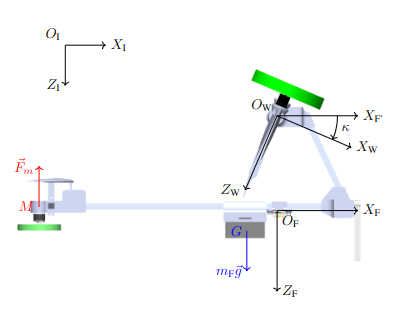
\includegraphics[width=0.6\columnwidth,angle=0,trim={0 0 0 0.5cm},clip]{figures/fram_side_colibri.png}
    \caption{Repère inertiel (I), du fuselage (F) et de l'aile (W) et forces agissant sur le drone Colibri.}
    \label{fig:colibri_frame_side}
\end{figure}


Nous devons aussi définir le vecteur de commande de dimension huit $\boldsymbol{u} = (u_{1},u_{2},u_{3},u_{4},\delta_{\text{l}},\delta_{\text{r}},u_{\text{tail}},\delta_{\text{tail}})$, où les actionneurs sont repérés en vert et rose sur la Figure \ref{fig:world_body}. Les actionneurs verts sont des groupes moteurs-hélices et les actionneurs rose sont des surfaces aérodynamiques. 

Il convient de noter que la vitesse angulaire $\boldsymbol{\omega} \in \real^{3}$ peut être obtenue à partir de la dérivée du quaternion $\dot{\boldsymbol{q}}$ en utilisant l'équation \cite[équation (2.7)]{udwadia-schutte} rappelée ici : 
\begin{align*}
    \boldsymbol{\omega} = \boldsymbol{H}(\boldsymbol{q}) \dot{\boldsymbol{q}} 
\end{align*}
où $\boldsymbol{H}(\boldsymbol{q}) \in \real^{3\times4}$ est une matrice définie par $\boldsymbol{H}(\boldsymbol{q}) = 2\begin{bmatrix}-\boldsymbol{\epsilon} & \eta \mathbb{I}_{3} - \skewsym{\boldsymbol{\epsilon}}\end{bmatrix}$.
Pour dériver les équations du mouvement, rappelons que  $\boldsymbol{R}_{i}(\boldsymbol{q}) \in \real^{3}, i = 1,2,3$ sont les trois colonnes d'une matrice de rotation associée au quaternion $q$, lesquelles définissent les matrices $\boldsymbol{L}_{\text{i}}^{\text{W}} \left( \boldsymbol{q}_{\text{W}} \right) = \frac{\partial \boldsymbol{R}_{i}}{\partial \boldsymbol{q}}(\boldsymbol{q}_{\text{W}}) \in \real^{3\times4}$, 
$\boldsymbol{L}_{\text{i}}^{\text{F}} \left( \boldsymbol{q}_{\text{F}} \right) = \frac{\partial \boldsymbol{R}_{i}}{\partial \boldsymbol{q}}(\boldsymbol{q}_{\text{F}}) \in \real^{3\times4}$ et
$\boldsymbol{L}_{\boldsymbol{O}_{\text{F}}^{\text{W}}} = \sum_{i=1}^{3} \boldsymbol{d}_{\text{FW}}(i) \boldsymbol{L}_{\text{i}}^{\text{F}} (\boldsymbol{q}_{\text{F}})$, $i \in {1,2,3}$, où $\boldsymbol{d}_{\text{FW}}(i)$ désigne la i-ème composante du vecteur $\boldsymbol{d}_{\text{FW}} = \boldsymbol{p}_{\text{W}} - \boldsymbol{p}_{\text{F}}$. Comme le point $\boldsymbol{O}_{\text{W}}$ est situé au centre de rotation de l'aile, la distance $\boldsymbol{d}_{\text{FW}}$ est une constante, puisque $\boldsymbol{O}_{\text{W}}$ et $\boldsymbol{O}_{\text{F}}$ appartiennent au même solide (le fuselage).

Nous en déduisons, avec l'homogénéité, $\dot{\boldsymbol{L}}_{\boldsymbol{O}_{\text{F}}^{\text{W}}} = \sum_{i=1}^{3} \boldsymbol{d}_{\text{FW}}(i) \boldsymbol{L}_{\text{i}}^{\text{F}} (\dot{\boldsymbol{q}}_{\text{F}})$. Avec ces définitions, les matrices de \eqref{eq:udwadia} sont :

\begin{align}
    \boldsymbol{M} = \begin{bmatrix}
        m_{\text{W}} \mathbb{I}_{3} & \mathbb{0}_{3 \times 4} & \mathbb{0}_{3} & \mathbb{0}_{3 \times 4}\\
        \mathbb{0}_{4 \times 3} & \boldsymbol{H}_{\text{W}}^\top \boldsymbol{J}_{\text{W}} \boldsymbol{H}_{\text{W}} & \mathbb{0}_{4 \times 3} & \mathbb{0}_{4}\\
        \mathbb{0}_{3} & \mathbb{0}_{3 \times 4} & m_{\text{F}} \mathbb{I}_{3} & \mathbb{0}_{3 \times 4} \\
        \mathbb{0}_{4 \times 3} & \mathbb{0}_{4 } & \mathbb{0}_{4 \times 3} & \boldsymbol{H}_{\text{F}}^\top \boldsymbol{J}_{\text{F}} \boldsymbol{H}_{\text{F}}    \end{bmatrix}\in \real^{14\times14},
\end{align}
où nous avons noté $\boldsymbol{H}_{\text{W}} = \boldsymbol{H}(\boldsymbol{q}_{\text{W}})$, $\boldsymbol{H}_{\text{F}} = \boldsymbol{H}(\boldsymbol{q}_{\text{F}})$, et
\begin{align}
    \label{eq:Q}
    \boldsymbol{Q} = \begin{bmatrix}
            m_{\text{W}} g \boldsymbol{e}_3 + \boldsymbol{R}(\boldsymbol{q}_{\text{W}}) \boldsymbol{F}_{\text{W}}(\boldsymbol{x}, \boldsymbol{u})\\
            -2\dot{\boldsymbol{H}}_{\text{W}}^\top \boldsymbol{J}_{\text{W}} \dot{\boldsymbol{H}}_{\text{W}} \dot{\boldsymbol{q}}_{\text{W}} + \boldsymbol{H}_{\text{W}}^\top \boldsymbol{M}_{\text{W}}(\boldsymbol{x}, \boldsymbol{u})\\
            m_{\text{F}} g \boldsymbol{e}_3 + \boldsymbol{R}(\boldsymbol{q}_{\text{F}}) \boldsymbol{F}_{\text{F}}(\boldsymbol{u})\\
            -2\dot{\boldsymbol{H}}_{\text{F}}^\top \boldsymbol{J}_{\text{F}} \dot{\boldsymbol{H}}_{\text{F}} \dot{\boldsymbol{q}}_{\text{F}} + \boldsymbol{H}_{\text{F}}^\top \boldsymbol{M}_{\text{F}}(\boldsymbol{u})\\
        \end{bmatrix} \in \real^{14},
\end{align}


où $\dot{\boldsymbol{H}}_{\text{W}}$ désigne $\boldsymbol{H}(\dot{\boldsymbol{q}}_{\text{W}})$, coïncidant avec la dérivée temporelle de $\boldsymbol{H}(\boldsymbol{q}_{\text{W}})$ et $\dot{\boldsymbol{H}}_{\text{F}}$ désigne $\boldsymbol{H}(\dot{\boldsymbol{q}}_{\text{F}})$, coïncidant avec la dérivée temporelle de $\boldsymbol{H}(\boldsymbol{q}_{\text{F}})$. De plus, $\boldsymbol{F}_{\text{W}}(x)$ et $\boldsymbol{M}_{\text{b}}(x)$ représentent respectivement toutes les forces et tous les moments agissant sur l'aile. Leur expression est tirée de \cite[équations (45) et (57)]{lustosaHal-03035938} où est développée la $\phi$-théorie, paramétrage qui permet de soustraire les angles classiques d'incidence et de dérapage et d'éviter la singularité du vol stationnaire. De manière similaire aux équations \eqref{eq:Fbdarko} et \eqref{eq:Mbdarko} exprimant les forces et les moments agissant sur DarkO, nous pouvons exprimer $\boldsymbol{F}_{\text{W}}(x)$ et $\boldsymbol{M}_{\text{b}}(x)$ relatifs à l'aile de Colibri.

Chaque hélice génère une poussée $\boldsymbol{T}_i$ orientée dans la direction $-z{\text{W}}$ du repère de l'aile et un moment $\boldsymbol{N}_i$ selon le même axe :
\begin{align}
\label{eq:thrustcolibri}
\boldsymbol{T}_{i} \!:=\! \begin{bmatrix} \tau_{i} \\ 0 \\ 0 \end{bmatrix} \!:=\!
\begin{bmatrix} k_{\text{f}}\omega_{i}^{2} \\ 0 \\ 0 \end{bmatrix}\! , \;
\boldsymbol{N}_{i} \!:=\! (-1)^{i}  \frac{k_{\text{m}} }{k_{\text{f}}}\boldsymbol{T}_{i}, \quad i=1,2,3,4,\text{tail} .
\end{align}  

La position de chaque élevon $\delta_i \in \real$ est assignée par un servomoteur qui impose un niveau d'efficacité (en termes de déviation du courant d'air) quantifié par deux matrices antisymétriques :
\begin{align}
\label{eq:elevons_efficiency_colibri}
    \boldsymbol{\Delta}^{\text{f}}_{i} \!:=\! \begin{bmatrix} 0 & 0 & \xi_{\text{f}}\delta_{i} \\ 0 & 0 & 0 \\ -\xi_{\text{f}}\delta_{i} & 0 & 0 \end{bmatrix}\! ,\;
    \boldsymbol{\Delta}^{\text{m}}_{i} \!:=\! \begin{bmatrix} 0 & 0 & \xi_{\text{m}}\delta_{i} \\ 0 & 0 & 0 \\ -\xi_{\text{m}}\delta_{i} & 0 & 0 \end{bmatrix} \!, \quad i=\text{l},\text{r}.
\end{align}
 Les paramètres constants $k_{\text{f}}$, $k_{\text{m}}$, $\xi_{\text{f}}$, $\xi_{\text{m}}$ apparaissant dans \eqref{eq:thrust} et \eqref{eq:elevons_efficiency} sont listés dans la Table~\ref{tab:pars_colibri}.


Avec les quantités ci-dessus, nous pouvons nous inspirer de la dynamique donnée dans  \cite[eqns (97),~(98)]{lustosaHal-03035938} et exprimer $\boldsymbol{F}_{\text{W}}(x,u)$ et $\boldsymbol{M}_{\text{W}}(x,u)$ dans \eqref{eq:Q} comme :
\begingroup
    \allowdisplaybreaks
    \begin{align}
    \nonumber
    \boldsymbol{F}_{\text{W}}(x,u) :={}&  \sum_{i=1}^{4} \boldsymbol{T}_{i} + \frac{S_{\text{wet}}}{4S_{\text{p}}} \boldsymbol{\Phi}^{\text{(fv)}} \Big( (\boldsymbol{\Delta}^{\text{f}}_1 - \mathbb{I}_{3} ) (\boldsymbol{T}_{1}+\boldsymbol{T}_{2}) + ( \boldsymbol{\Delta}^{\text{f}}_2 - \mathbb{I}_{3}) (\boldsymbol{T}_{3}+\boldsymbol{T}_{4})\Big) \\ 
    \nonumber
        &+ \frac{1}{4} \rho S  \boldsymbol{\Phi}^{\text{(fv)}} \Big(\boldsymbol{\Delta}^{\text{f}}_1+ \boldsymbol{\Delta}^{\text{f}}_2 - 2 \mathbb{I}_{3} \Big) \lVert \boldsymbol{v_{\text{b}}} \rVert \boldsymbol{v_{\text{b}}}\\
        &+ \frac{1}{4} \rho S \boldsymbol{\Phi}^{\text{(mv)}} \Big(\boldsymbol{\Delta}^{\text{f}}_1 + \boldsymbol{\Delta}^{\text{f}}_2 - 2\mathbb{I}_{3}\Big) \boldsymbol{B} \lVert \boldsymbol{v_{\text{b}}} \rVert  \boldsymbol{\omega}_{\text{b}}, \label{eq:FbColibri}
    \end{align}
\endgroup
% \boldsymbol{N}_{2} + \boldsymbol{N}_{3} + \boldsymbol{N}_{4}  + \boldsymbol{T}_{2} + \boldsymbol{T}_{3} + \boldsymbol{T}_{4} 
\begingroup
    \allowdisplaybreaks
    \begin{align} 
    \nonumber
    \boldsymbol{M}_{\text{W}}(x,u) :&= \sum_{i=1}^{4} \boldsymbol{N}_{i} ++\skewsym{\smallm{p_x\\ p_{y1}\\ 0}} \boldsymbol{T}_{1} +\skewsym{\smallm{p_x\\ p_{y2}\\ 0}} \boldsymbol{T}_{2} + \skewsym{\smallm{p_x\\ - p_{y3}\\ 0}} \boldsymbol{T}_{3} + \skewsym{\smallm{p_x\\ - p_{y4}\\ 0}} \boldsymbol{T}_{4}\\
        \nonumber
    &- \frac{S_{\text{wet}}}{4S_{\text{p}}} \bigg( \boldsymbol{B} \boldsymbol{\Phi}^{\text{(mv)}} (\boldsymbol{\Delta}^{\text{m}}_1- \mathbb{I}_{3} ) + \skewsym{\smallm{0 \\ a_y \\ 0}} \boldsymbol{\Phi}^{\text{(fv)}} (\boldsymbol{\Delta}^{\text{m}}_1 +\mathbb{I}_{3} ) \bigg) (\boldsymbol{T}_{1}+\boldsymbol{T}_{2}) \\
        \nonumber
    & - \frac{S_{\text{wet}}}{4S_{\text{p}}} \bigg( \boldsymbol{B} \boldsymbol{\Phi}^{\text{(mv)}} (\boldsymbol{\Delta}^{\text{m}}_2 - \mathbb{I}_{3} ) +  \skewsym{\smallm{0 \\ - a_y \\ 0}} \boldsymbol{\Phi}^{\text{(fv)}} (\boldsymbol{\Delta}^{\text{m}}_2 + \mathbb{I}_{3}) \bigg) (\boldsymbol{T}_{3}+\boldsymbol{T}_{4}) \\
        \nonumber
    & + \frac{1}{4} \rho S  \bigg( \Big(\skewsym{\smallm{0 \\ a_y \\ 0}} \!\!\! \boldsymbol{\Phi}^{\text{(fv)}}  + \boldsymbol{B} \boldsymbol{\Phi}^{\text{(mv)}} \Big) \boldsymbol{\Delta}^{\text{m}}_1 \\
        \nonumber
    &  + \Big( \skewsym{\smallm{0 \\ - a_y \\ 0}} \!\!\! \boldsymbol{\Phi}^{\text{(fv)}} + \boldsymbol{B} \boldsymbol{\Phi}^{\text{(mv)}}  \Big) \boldsymbol{\Delta}^{\text{m}}_2 - 2 \boldsymbol{B} \boldsymbol{\Phi}^{\text{(mv)}}  \bigg) \lVert \boldsymbol{v_{\text{b}}} \rVert \boldsymbol{v_{\text{b}}} \\
        \nonumber
    & +\frac{1}{4} \rho S \bigg(\!\! \Big(\!\! \skewsym{\!\smallm{0 \\ a_y \\ 0}\!}\!\!\! \boldsymbol{\Phi}^{\text{(mv)}} \! + \! \boldsymbol{B} \boldsymbol{\Phi}^{\text{(m$\omega$)}} \Big) \boldsymbol{\Delta}^{\text{m}}_1 \\
    & +  \Big(\!\! \skewsym{\!\smallm{0 \\ - a_y \\ 0}\!} \!\!\! \boldsymbol{\Phi}^{\text{(mv)}} \! + \! \boldsymbol{B} \boldsymbol{\Phi}^{\text{(m$\omega$)}}  \Big) \boldsymbol{\Delta}^{\text{m}}_2 - 2 \boldsymbol{B} \boldsymbol{\Phi}^{\text{(m$\omega$)}}\!  \bigg)\!  \boldsymbol{B}  \lVert \boldsymbol{v_{\text{b}}} \rVert  \boldsymbol{\omega}_{\text{b}} , \label{eq:MbColibri}
    \end{align}
\endgroup
où $\boldsymbol{v}_{\text{b}} := \boldsymbol{R}^\top(\boldsymbol{q}) (\boldsymbol{v}-\boldsymbol{w})$ représente la vitesse de l'air vue par le drone et exprimée dans le repère du corps. Dans \cite{lustosaHal-03035938}, la valeur $\lVert \boldsymbol{v_{\text{b}}} \rVert$, apparaissant dans les expressions de  $\boldsymbol{F}_{\text{b}}$ et $\boldsymbol{M}_{\text{b}}$, est remplacée par la valeur $\eta = \sqrt{\lVert \boldsymbol{v_{\text{b}}} \rVert^{2} + \mu c^{2} \lVert \boldsymbol{\omega}_{\text{b}} \rVert^{2}}$, avec $\mu \in \real$ étant un paramètre lié à l'identification du modèle. Toutefois, dans le cas de Colibri, l'identification fournit $\mu = 0$. 

Dès lors, nous présentons ici une description simplifiée. La matrice des coefficients aérodynamiques constants 
$\boldsymbol{\Phi}:= \begin{bmatrix} \boldsymbol{\Phi}^{\text{(fv)}} & {\boldsymbol{\Phi}^{\text{(mv)}}}^\top \\ \boldsymbol{\Phi}^{\text{(mv)}} & \boldsymbol{\Phi}^{\text{(m$\omega$)}} \end{bmatrix} \in \real^{6 \times 6}$, est définie dans \cite[eqs. (6)--(9)]{olszaneckibarthHal-02542982} comme $ \boldsymbol{\Phi}^{\text{(fv)}} \!:=\! \diag(C_{\text{d}},C_{y}, C_{\ell})$ et
\begin{align*}
&\left[ \begin{array}{c|c}
    \boldsymbol{\Phi}^{\text{(mv)}}  &  \boldsymbol{\Phi}^{\text{(m$\omega$)}} 
\end{array}\right] :=\\ 
&\left[ \begin{array}{ccc|ccc}
    0 & 0 & 0    &                                          0.1396 & 0 & 0.0573 \\
    0 & 0 & \!\!\!\!\! -\frac{\Delta_{\text{r}}}{c}C_{\ell} &    0 &  0.6358  & 0 \\
    0 & 0 & 0 &     0.0405 & 0 & 0.0019 
\end{array}\right].
\end{align*}




Enfin, $\boldsymbol{F}_{\text{F}} = \boldsymbol{F}_{m}$ et $\boldsymbol{M}_{\text{F}}$ représentent respectivement l'ensemble des forces et moments non gravitationnels agissant sur le fuselage exprimés dans le repère $O_{\text{W}}$. En particulier, $\boldsymbol{F}_{m} = - k_{\text{p}} {u_{\text{tail}}}^{2}$ est la force générée par le moteur situé à l'arrière du fuselage et $u_{\text{tail}}$ est la vitesse de rotation du moteur.

Nous utilisons le théorème fondamental de la statique et nous isolons le fuselage. Les deux moments qui agissent sur le fuselage sont le couple dû à la force de poussée du moteur (en rouge sur la Figure \eqref{fig:colibri_frame_side}) et le couple dû à la position du centre de gravité du fuselage (en bleu sur la Figure \eqref{fig:colibri_frame_side}). Il en resulte l'équation suivante :

\begin{align}
    \label{eq:momentfuselage}
    \boldsymbol{M}_{\text{F}} =  m_{\text{F}} g \boldsymbol{e}_3 \times \boldsymbol{d}_{\text{G}O_{\text{W}}} + \boldsymbol{F}_{m} \times \boldsymbol{d}_{\text{M}O_{\text{W}}},
\end{align}
où $\boldsymbol{d}_{\text{M}O_{\text{W}}}$ est la distance entre l'emplacement du moteur et le centre de rotation et $\boldsymbol{d}_{\text{G}O_{\text{W}}}$ est la distance entre l'emplacement du centre de gravité du fuselage et le centre de rotation.


L'ensemble des contraintes, associé à la non-minimalité de l'état $(\boldsymbol{x},\boldsymbol{v})$ et à la liaison pivot entre les deux corps, est donné par :
\begin{align}
    \label{eq:contraintes}
    \left\{
    \begin{aligned}
    &\varphi_{1} \coloneqq \boldsymbol{q}_{\text{W}}^\top \boldsymbol{q}_{\text{W}} - 1 = 0\\
    &\varphi_{2} \coloneqq \boldsymbol{q}_{\text{F}}^\top \boldsymbol{q}_{\text{F}} - 1 = 0\\
    &\varphi_{3} \coloneqq \boldsymbol{R}_{2}(q_{\text{W}})^\top \boldsymbol{R}_{3}(q_{\text{F}}) = 0\\
    &\varphi_{4} \coloneqq \boldsymbol{R}_{2}(q_{\text{W}})^\top \boldsymbol{R}_{1}(q_{\text{F}}) = 0\\
    &\boldsymbol{\varphi}_{5} \coloneqq \boldsymbol{p}_{\text{F}} + \boldsymbol{d}_{\text{FA}} + \boldsymbol{p}_{\text{W}} = 0
    \end{aligned}.
    \right.
\end{align}

Les deux premières contraintes imposent la norme unitaire des quaternions $\boldsymbol{q}_{\text{F}}$ et $\boldsymbol{q}_{\text{W}}$.
Les troisième et quatrième contraintes sont liées à une contrainte pivot, c'est-à-dire que l'orthogonalité de deux vecteurs est imposée. La dernière est une contrainte de position, de sorte que le point du centre de rotation de l'aile coïncide avec le point défini dans le fuselage. Cette contrainte est basée sur une fermeture géométrique tridimensionnelle.
Il est plus commode d'exprimer l'ensemble des contraintes sous la forme d'un système dynamique stable convergeant vers zéro. Nous convertissons donc chacune des contraintes sous la forme suivante :
\begin{align}
    \ddot{\varphi_{i}} + \delta_{1} \dot{\varphi_{i}}  + \delta_{2} \varphi_{i} = 0, i \in {1,2,3,4,5},
\end{align}

avec les sélections $(\delta_{1}, \delta_{2}) = (0.5,~8)$ étant les coefficients d'un polynôme stable, de sorte que, quelle que soit la sélection $\varphi_{i}(0) = 0$, nous ayons $\lim\limits_{t \to \infty} \varphi_{i}(t) = 0$. En différenciant deux fois les contraintes \eqref{eq:contraintes} et en les factorisant sous la forme de l'équation \eqref{eq:contrainteAB}, nous obtenons l'expression de $\boldsymbol{A}(\boldsymbol{x},\dot{\boldsymbol{x}})$ reportée dans l'équation \eqref{eq:A_contraint} et de $\boldsymbol{B}(\boldsymbol{x},\dot{\boldsymbol{x}})$ reportée dans l'équation \eqref{eq:b_contraint}.

\begin{align}
\label{eq:A_contraint}
\boldsymbol{A} = \begin{bmatrix}
            \mathbb{0}_{1 \times 3} & \boldsymbol{q}_{\text{W}}^\top & \mathbb{0}_{1 \times 3} & \mathbb{0}_{1 \times 4}\\
            \mathbb{0}_{1 \times 3} & \mathbb{0}_{1 \times 4} & \mathbb{0}_{1 \times 3} & \boldsymbol{q}_{\text{F}}^\top\\
            \mathbb{0}_{1 \times 3} & \boldsymbol{R}_{3}(\boldsymbol{q}_{\text{F}})^\top \boldsymbol{L}_{2}^{\text{W}}( \boldsymbol{q}_{\text{W}} ) & \mathbb{0}_{1 \times 3} & \boldsymbol{R}_{2}(\boldsymbol{q}_{\text{W}})^\top \boldsymbol{L}_{3}^{\text{F}}( \boldsymbol{q}_{\text{F}} ) \\
            \mathbb{0}_{1 \times 3} & \boldsymbol{R}_{1}(\boldsymbol{q}_{\text{F}})^\top \boldsymbol{L}_{2}^{\text{W}}( \boldsymbol{q}_{\text{W}} ) & \mathbb{0}_{1 \times 3} & \boldsymbol{R}_{2}(\boldsymbol{q}_{\text{W}})^\top \boldsymbol{L}_{3}^{\text{F}}( \boldsymbol{q}_{\text{F}} ) \\
            \mathbb{I}_{3} & \boldsymbol{L}_{O_{\text{F}}^{\text{W}}} & -\mathbb{I}_{3} & \mathbb{0}_{3 \times 4}
        \end{bmatrix}
\end{align}

\begin{align}
    \label{eq:b_contraint}
    \boldsymbol{B} = \begin{bmatrix}
            -\delta_{1} \boldsymbol{q}_{\text{W}}^\top \dot{\boldsymbol{q}}_{\text{W}} - \frac{\delta_{2}}{2} (\boldsymbol{q}_{\text{W}}^\top \boldsymbol{q}_{\text{W}} -1) - \dot{\boldsymbol{q}}_{\text{W}}^\top \dot{\boldsymbol{q}}_{\text{W}} \\
            -\delta_{1} \boldsymbol{q}_{\text{F}}^\top \dot{\boldsymbol{q}}_{\text{F}} - \frac{\delta_{2}}{2} (\boldsymbol{q}_{\text{F}}^\top \boldsymbol{q}_{\text{F}} -1) - \dot{\boldsymbol{q}}_{\text{F}}^\top \dot{\boldsymbol{q}}_{\text{F}} \\
            B_{3}\\
            B_{4}\\
            \dot{\boldsymbol{L}}_{O_{\text{F}}^{\text{W}}} \dot{\boldsymbol{q}}_{\text{F}}  - \delta_{1}( \boldsymbol{v}_{\text{W}} + \dot{\boldsymbol{L}}_{O_{\text{F}}^{\text{W}}} \dot{\boldsymbol{q}}_{\text{W}} - \boldsymbol{v}_{\text{F}}) - \delta_{1}\boldsymbol{\varphi}_{5}
        \end{bmatrix}.
\end{align}
avec 
\begin{multline*}
    B_{3} = -\boldsymbol{R}_{3}(\boldsymbol{q}_{\text{F}})^\top \dot{\boldsymbol{L}}_{2}^{\text{W}}\dot{\boldsymbol{q}}_{\text{W}} - \boldsymbol{R}_{2}(\boldsymbol{q}_{\text{W}})^\top \dot{\boldsymbol{L}}_{3}^{\text{F}} \dot{\boldsymbol{q}}_{\text{F}} - 2\dot{\boldsymbol{q}}_{\text{W}}^\top {\boldsymbol{L}_{2}^{\text{W}}}^\top \boldsymbol{L}_{3}^{\text{F}} \dot{\boldsymbol{q}}_{\text{F}}\\ - \delta_{1}(\boldsymbol{R}_{3}(\boldsymbol{q}_{\text{F}})^\top \boldsymbol{L}_{2}^{\text{W}}\dot{\boldsymbol{q}}_{\text{W}} +  \boldsymbol{R}_{2}(\boldsymbol{q}_{\text{W}})^\top \boldsymbol{L}_{3}^{\text{F}} \dot{\boldsymbol{q}}_{\text{F}} ) - \delta_{2}\varphi_{3}
\end{multline*}
et 
\begin{multline*}
    B_{4} = -\boldsymbol{R}_{1}(\boldsymbol{q}_{\text{F}})^\top \dot{\boldsymbol{L}}_{2}^{\text{W}}\dot{\boldsymbol{q}}_{\text{W}} - \boldsymbol{R}_{2}(\boldsymbol{q}_{\text{W}})^\top \dot{\boldsymbol{L}}_{1}^{\text{F}} \dot{\boldsymbol{q}}_{\text{F}} - 2\dot{\boldsymbol{q}}_{\text{W}}^\top {\boldsymbol{L}_{2}^{\text{W}}}^\top \boldsymbol{L}_{1}^{\text{F}} \dot{\boldsymbol{q}}_{\text{F}} \\- \delta_{1}(\boldsymbol{R}_{1}(\boldsymbol{q}_{\text{F}})^\top \boldsymbol{L}_{2}^{\text{W}}\dot{\boldsymbol{q}}_{\text{W}} +  \boldsymbol{R}_{2}(\boldsymbol{q}_{\text{W}})^\top \boldsymbol{L}_{1}^{\text{F}} \dot{\boldsymbol{q}}_{\text{F}} ) - \delta_{2} \varphi_{4}.
\end{multline*}

La simulation d'un drone reste complexe, car il est naturellement instable. Nous avons choisi d'utiliser la loi de contrôle proposée dans \ref{sec:h_inf6DOF_multi} pour stabiliser le système. Ce contrôle stabilise l'aile. Une autre loi de contrôle basée sur une rétroaction proportionnelle-dérivée stabilise le fuselage pour le maintenir horizontal, développée dans la section \ref{sec:stabfus}. Les résultats de la simulation en boucle fermée sont présentés à la Figure~\ref{fig:sim_colibri}.

\begin{figure}[ht!]
\centering
    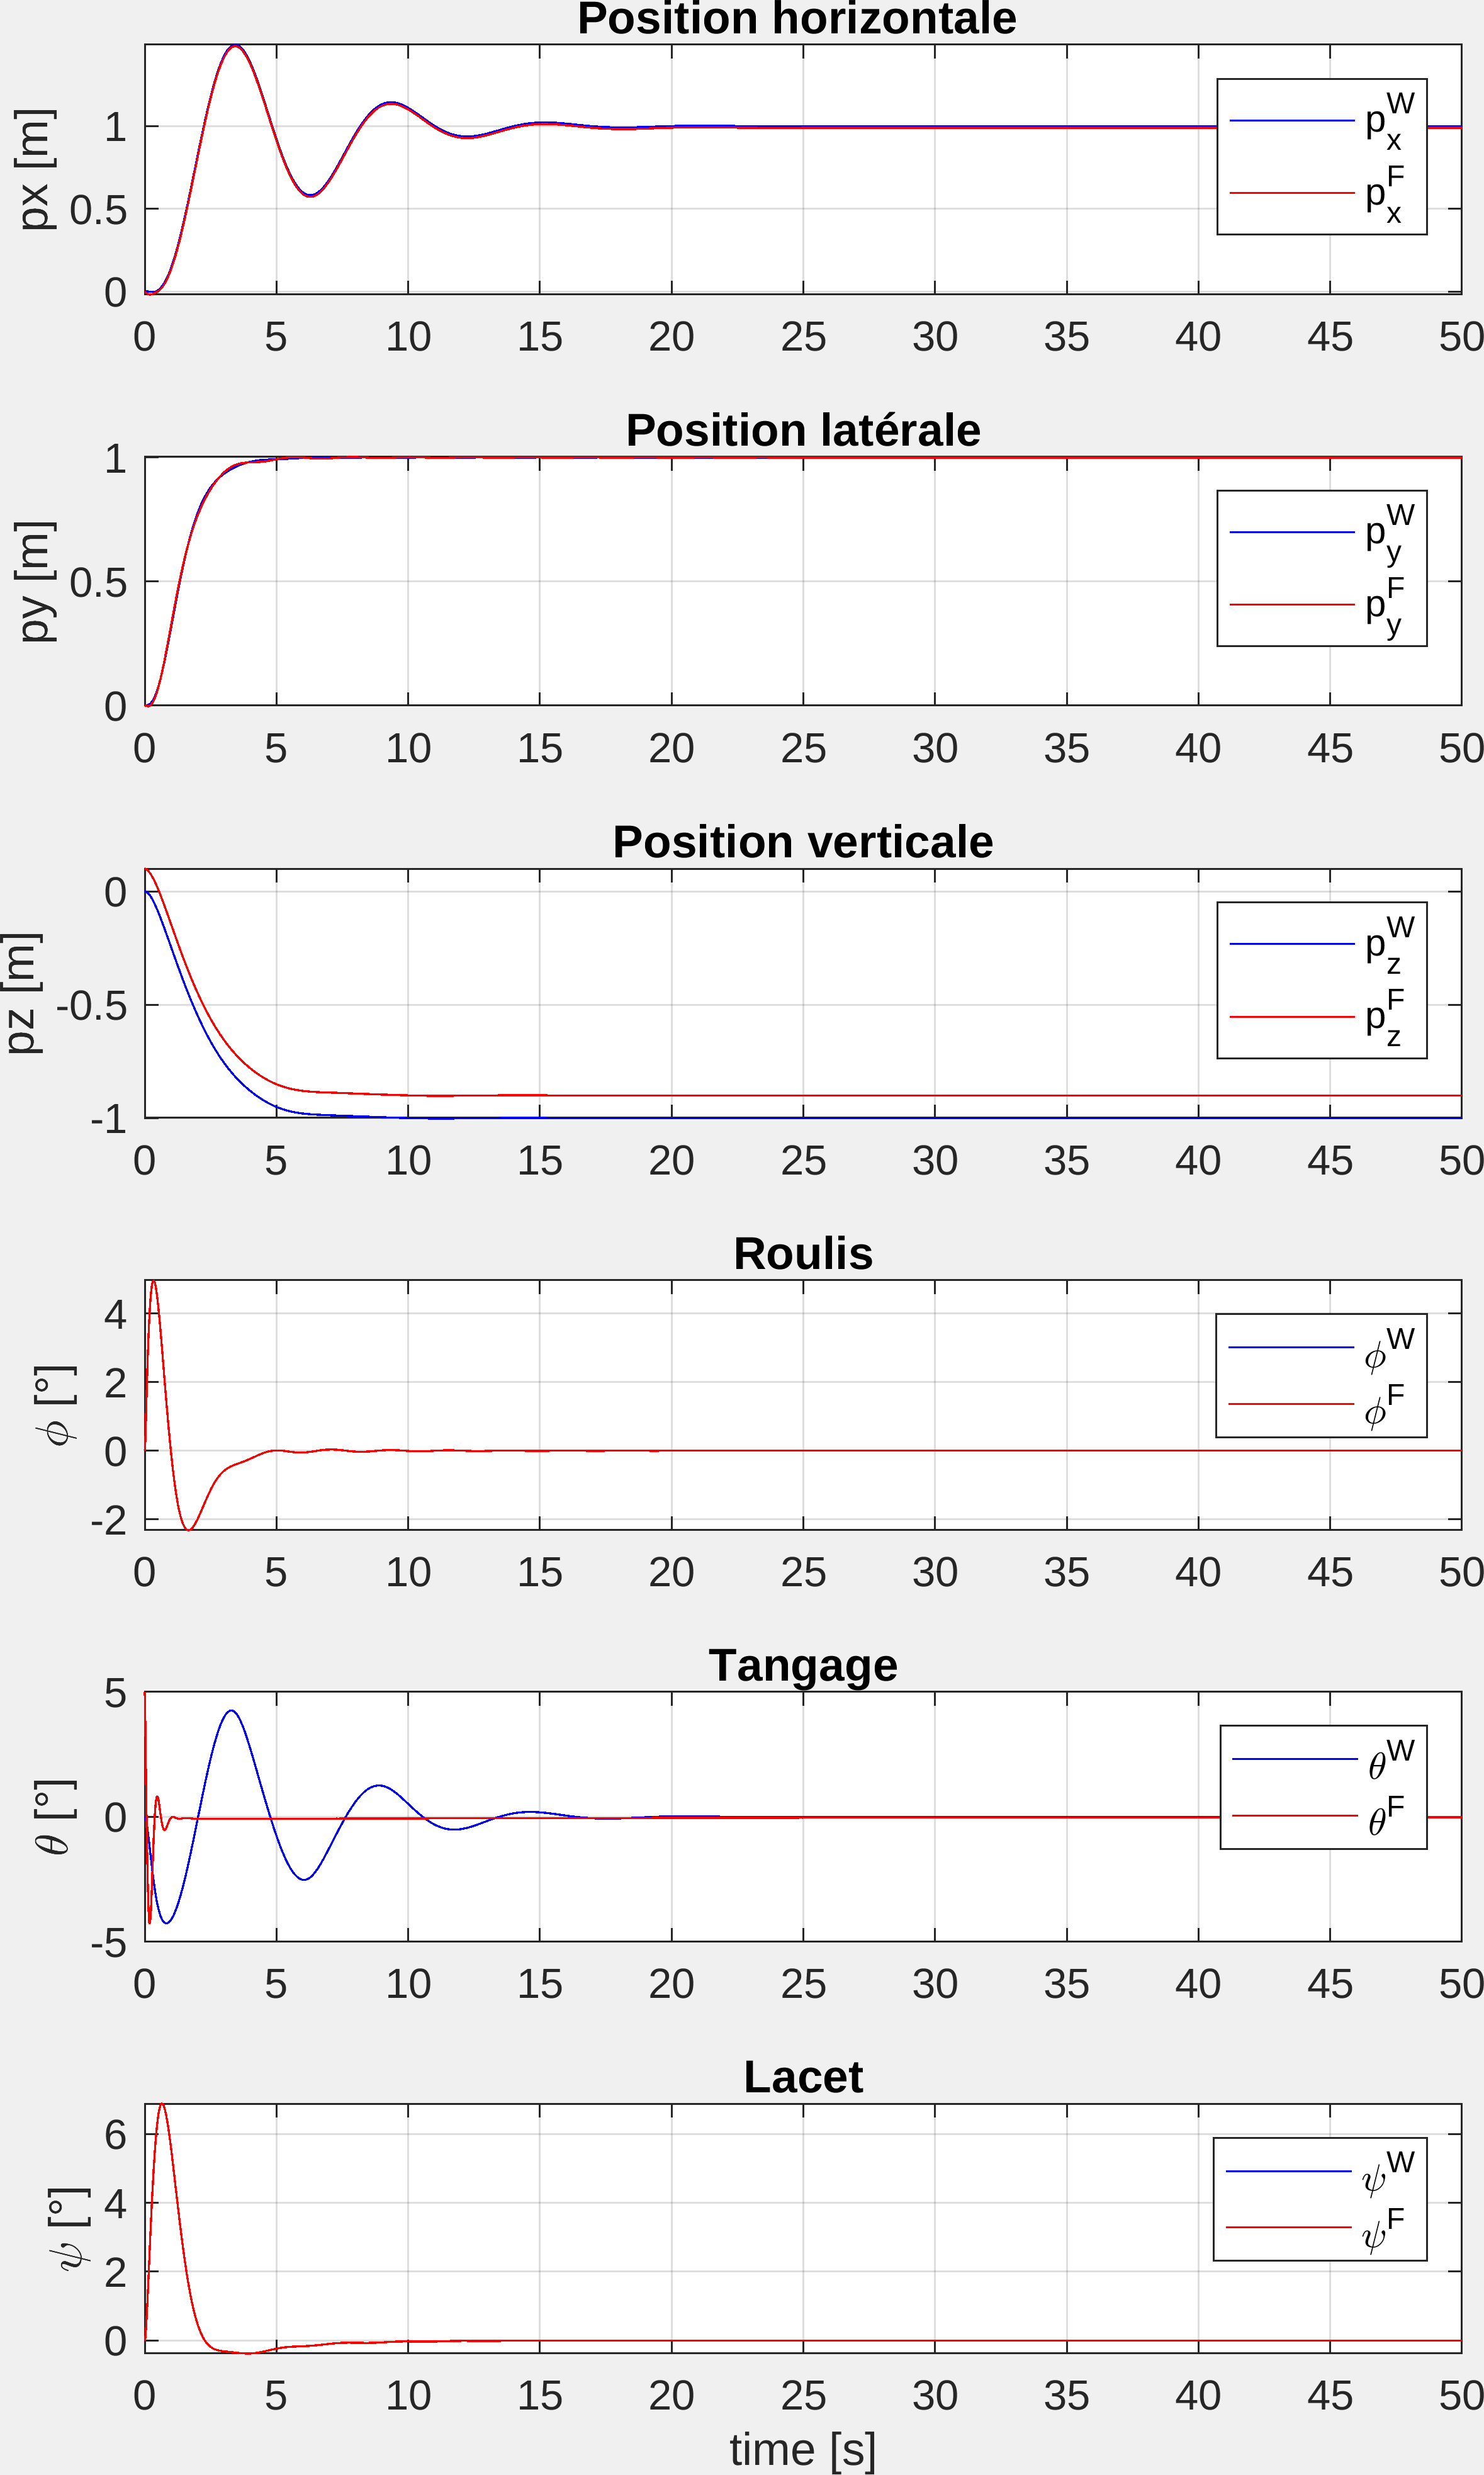
\includegraphics[width=0.6\columnwidth,angle=0]{figures/colibri_sim.png}
    \caption{Simulation de la position et de l'orientation du drone multicorps Colibri en boucle fermée avec un contrôleur à double boucle. }
    \label{fig:sim_colibri}
\end{figure}

En considérant les degrés de liberté de la liaison pivot, le couplage entre les deux corps est clairement visible sur les trois graphiques du bas. En effet, les angles de roulis et de lacet $(\phi_{\text{F}}, \psi_{\text{F}})$ et $(\phi_{\text{W}}, \psi_{\text{W}})$ du fuselage et de l'aile coïncident parfaitement, alors que les angles de tangage $(\theta_{\text{F}}, \theta_{\text{F}})$ sont différents.

{\color{blue}
    Par la suite, nous souhaitons réaliser des expérimentations avec un système réel. Nous devons donc étudier la possibilité d'obtention de l'estimation des corps pour stabiliser le drone.
}






\section{Estimation d'état}\label{sec:stateEst}

{\color{blue}
    Un des problèmes engendré par cette architecture multicorps est l'estimation de l'état de chacun des composants.
}


Pour stabiliser ce système de drone à deux corps, il est nécessaire de connaître la position et l'orientation des deux corps. Grâce à la liaison pivot entre l'aile et le fuselage, la différence entre l'orientation de l'aile et l'orientation du fuselage est simplement une rotation autour de l'axe de tangage de l'aile. Les deux autres orientations (roulis et lacet) coïncident. La position du centre de gravité du fuselage peut être déduite de la position du centre de gravité de l'aile et de l'angle entre le fuselage et l'aile. Cet angle est mesuré par un codeur rotatif en quadrature (CUI Devices AMT22, codeurs absolus, 12 bits, SPI), qui renvoie une mesure angulaire quantifiée avec un pas de \SI{0,09}{\degree}. Compte tenu de cette mesure angulaire, nous examinons ci-dessous l'estimation des informations relatives à la vitesse, afin de reconstruire l'état du drone.
\nomenclature[]{\(SPI\)}{Bus de données série synchrone \textit{Serial Peripheral Interface}}

\subsection{Placement des capteurs}
\label{subsec:sens_pos}
Une première question concerne l'emplacement des capteurs : l'IMU (accéléromètre, gyroscope et magnétomètre) peut être installée sur le fuselage ou sur l'aile. 
L'installation de l'IMU sur l'aile permet d'effectuer les mesures directement dans le référentiel souhaité, mais les mesures sont plus bruitées car l'IMU est attachée à la structure supportant les moteurs. Compte tenu de la taille des ailes, leur flexibilité peut générer des résonances et perturber les mesures. 

L'installation de l'IMU sur le fuselage réduit les vibrations, mais implique que les mesures soient transformées dans le référentiel de l'aile. La transformation correspondante peut être calculée à partir de la mesure de l'encodeur rotatif, qui fournit l'angle entre l'aile et le fuselage, ainsi qu'à partir des mesures prises avec le logiciel de CAO, qui fournissent des informations précises sur les distances entre les référentiels de l'aile et du fuselage. Notre choix final est de fixer l'IMU au fuselage. Une autre considération est que la carte de pilotage automatique, qui a déjà une IMU intégrée, est également supposée être connectée à la charge utile et à d'autres capteurs fixés sur fuselage. Il s'agit donc de limiter le nombre de câbles au point de pivot pour les commandes des actionneurs et l'alimentation électrique.

\nomenclature[]{\(CAO\)}{Conception assistée par ordinateur}

\subsection{Estimation de la vitesse angulaire}

Comme expliqué ci-dessus, nous pouvons mesurer l'angle $\kappa \in \real$ entre l'aile et le fuselage à l'aide de l'encodeur rotatif. Ensuite, pour estimer la vitesse angulaire, nous utilisons un observateur grand gain proposé dans \cite{203613} (voir également \cite{1032320} pour l'utilisation d'observateurs grand gain pour estimer les dérivées temporelles). Cette méthode est préférable à une dérivée par différence finie, car les informations quantifiées générées par l'encodeur rotatif peuvent donner lieu à du bruit numérique dans les valeurs estimées de vitesse angulaire.


Désignons par $\kappa \in \real$ l'angle mesuré, par $\omega_{\kappa} := \dot \kappa  \in \real$ sa dérivée à estimer, et par $\boldsymbol{\xi} = [\kappa,~\omega_{\kappa}]^\top \in \mathbb{R}^2$ leur juxtaposition en un seul vecteur. Notons également $\hat{\boldsymbol{\xi}}$ l'estimation de $\boldsymbol{\xi}$ définie par :
%\xi = [\kappa,~\omega_{\kappa}]^\top \in \mathbb{R}^2, \quad 
\begin{align*}
    \hat{\boldsymbol{\xi}} = [\hat{\kappa},~\hat{\omega}_{\kappa}]^\top \in \mathbb{R}^2.
\end{align*}
Suivant \cite{203613}, la dynamique de l'estimateur est donnée par :
\begin{align}
\label{eq:high_dyn}
    \dot{\hat{\boldsymbol{\xi}}} =  \begin{bmatrix}0 & 1 \\ 0 & 0 \end{bmatrix} \hat{\boldsymbol{\xi}}+ \begin{bmatrix}\frac{k_{p}}{\epsilon_{\kappa}}  \\ \frac{k_{v}}{\epsilon_{\kappa}^{2}}  \end{bmatrix} (\kappa - \hat{\kappa}),
\end{align}
où $\kappa$ est la mesure angulaire récupérée du capteur, $k_{p}$ et $k_{v}$ sont deux gains scalaires positifs tels que l'équation caractéristique $s^{2} + k_{v} s + k_{p} = 0$ ait des racines à partie réelle négative. Pour notre estimateur, nous avons choisi $k_{p} = 1$ et $k_{v} = 1,3$ de manière à obtenir un facteur d'amortissement $\zeta = 0,65$ conduisant à une réponse légèrement sous-amortie comme compromis approprié entre un temps de montée rapide et une réponse légèrement oscillatoire. Le gain $\epsilon_{\kappa}$ peut être ajusté de manière pratique afin d'obtenir un compromis entre l'action de lissage (obtenue en augmentant $\epsilon_{\kappa}$) et la réduction du retard temporel
de l'estimateur (obtenue en réduisant $\epsilon_{\kappa}$). En outre, l'action de lissage de l'approche proposée atténue l'effet de la quantification de la mesure angulaire. Nous avons choisi $\epsilon_{\kappa} = 0,05$ pour nos expériences. La Figure~\ref{fig:high_gain} montre les résultats expérimentaux obtenus après la mise en œuvre du filtre grand gain \eqref{eq:high_dyn} dans le cas d'un vol générant des oscillations angulaires de grande amplitude.

Nous avons effectué une dérivation par différence finie (en vert) en post-traitement pour comparer les résultats. En raison de la nature quantifiée de l'encodeur rotatif, nous observons que la vitesse angulaire obtenue par différence finie est très bruitée. Nous constatons que le filtre grand gain permet d'estimer la vitesse angulaire avec plus de précisions (en rouge), bien qu'avec un léger retard. Grâce à l'ajout d'une IMU supplémentaire sur l'aile lors d'un essai en vol, il est possible de comparer l'estimation de la vitesse avec les mesures du gyroscope de l'aile (MPU9250), visibles sur le graphique du bas de la Figure~\ref{fig:high_gain} (trace bleue). Nous constations que les mesures du gyroscope sont quelque peu bruitées, notamment en raison des vibrations générées par les moteurs. 

\begin{figure}[ht!]
\centering
    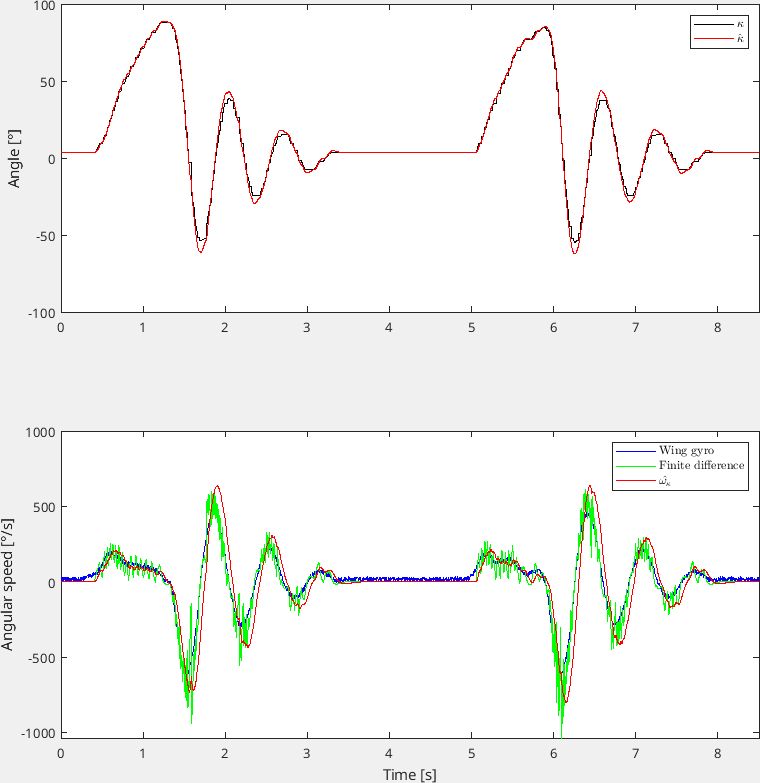
\includegraphics[width=0.8\columnwidth,angle=0]{figures/highGainFilter.png}
    \caption{Mesure de l'angle (noir, graphique du haut), mesure de la vitesse angulaire avec le gyroscope de l'aile (bleu, graphique du bas), estimation de la vitesse angulaire par différence finie (vert, graphique du bas) et estimation avec le filtre grand gain (courbes rouges).}
    \label{fig:high_gain}
\end{figure}

Afin d'effectuer la transformation nécessaire entre les repères, nous définissons le quaternion $\boldsymbol{q}_{\hat{\kappa}} \in {\mathbb S}^3$ suivant :
\begin{align}
\label{eq:rot_quat}
\boldsymbol{q}_{\hat{\kappa}} =  \left[\cos\left(\frac{\hat{\kappa}}{2}\right) ~ 0 ~ \sin\left(\frac{\hat{\kappa}}{2}\right) ~ 0 \right]^\top
\end{align}


\subsection{Estimation de l'état de l'aile}

Sur la base de l'angle estimé $\hat{\kappa}$ et de la vitesse angulaire estimée $\hat{\omega}_{\kappa}$, il est possible de transformer les mesures réalisées dans le repère du fuselage vers le repère de l'aile. Tous les capteurs sont installés sur la carte de l'autopilote, qui est elle-même fixée au fuselage. Cependant, nous voulons utiliser INDI pour stabiliser l'aile. Cette loi de contrôle nécessite donc des informations sur l'état du drone dans le repère de l'aile, où toutes les forces sont appliquées (aérodynamiques et de traction).

Deux solutions viables sont alors possibles : effectuer l'estimation d'état dans le repère du fuselage et faire pivoter l'estimation en utilisant l'estimation de l'angle $\hat{\kappa}$, ou faire pivoter les mesures brutes à l'avance pour les exprimer dans le repère l'aile, et ensuite effectuer l'estimation d'état dans ce dernier. 

Compte tenu de l'architecture actuelle du logiciel du système Paparazzi (voir Annexe \ref{sec:logiciel}), il est impossible d'avoir deux structures conjointes d'estimation de l'état. Il est donc complexe de mettre en œuvre la première solution, dans laquelle le contrôleur récupère directement l'estimation de l'état actuel. C'est pourquoi nous avons choisi d'estimer l'état de l'aile à partir des données mesurées sur le fuselage. À cette fin, nous détaillons ci-dessous les transformations pour les trois capteurs : gyroscope, accéléromètre et magnétomètre. 

Pour les mesures de la vitesse angulaire basées sur le gyroscope, nous pouvons calculer la vitesse angulaire de l'aile exprimée dans le repère de l'aile :
\begin{align}
    \label{eq:gyro_deplacement}
    \boldsymbol{\omega}_{\text{W}} = \boldsymbol{R}(\boldsymbol{q}_{\hat{\kappa}}) \left( \boldsymbol{\omega}_{gyro}^{\text{F}} + \begin{bmatrix}
    0\\ \omega_{\kappa} \\ 0
    \end{bmatrix}  \right) 
\end{align}
où $\boldsymbol{\omega}_{gyro}^{\text{F}}$ est la vitesse angulaire mesurée par le gyroscope sur le fuselage, exprimée dans le repère du fuselage, $\hat{\omega}_{\kappa}$ est la vitesse angulaire estimée de l'aile par rapport au fuselage, conformément à \eqref{eq:high_dyn}, et $\boldsymbol{q}_{\hat{\kappa}}$ est le quaternion défini dans \eqref{eq:rot_quat}.
L'expression \eqref{eq:gyro_deplacement} est similaire à une composition de vitesse angulaire et à un changement du repère.

Pour la mesure de l'accélération avec l'accéléromètre, nous pouvons utiliser la relation de l'équation \eqref{eq:accel_deplacement}, qui est obtenue à partir du théorème de transport du taux de variation \cite{brizard2004motion}, où nous trouvons le terme d'accélération d'Euler $\dot{\boldsymbol{\omega}_{\text{F}}} \times \boldsymbol{d}_{AF}$  et le terme d'accélération centripète $\boldsymbol{\omega}_{\text{F}} \times ( \boldsymbol{\omega}_{\text{F}} \times  \boldsymbol{d}_{AF})$. L'accélération de Coriolis $2\boldsymbol{\omega}_{\text{F}} \times \frac{d (\boldsymbol{d}_{\text{FW}})}{d t}\Bigr|_{O_{\text{F}}}$ et le taux d'accélération $\frac{d^{2} (\boldsymbol{d}_{\text{FW}})}{d^{2} t}\Bigr|_{O_{\text{F}}}$ sont nuls car $\boldsymbol{d}_{\text{FW}}$ est constant.

\begin{align}
    \label{eq:accel_deplacement}
    \boldsymbol{a}_{\text{W}} = \boldsymbol{R}(\boldsymbol{q}_{\hat{\kappa}}) \left( \boldsymbol{a}_{acc}^{F} + \dot{\boldsymbol{\omega}}_{gyro}^{F} \times \boldsymbol{d}_{\text{FW}} + \boldsymbol{\omega}_{gyro}^{F} \times ( \boldsymbol{\omega}_{gyro}^{F} \times  \boldsymbol{d}_{\text{FW}}) \right) 
\end{align}
où $\boldsymbol{a}_{acc}^{F} \in \real^{3}$ est l'accélération mesurée par l'accéléromètre sur le fuselage, exprimée dans le repère du fuselage et $\boldsymbol{\omega}_{gyro}^{F} \in \real^{3}$ est la vitesse angulaire du fuselage, identique à l'équation \eqref{eq:gyro_deplacement}. L'accélération angulaire $\dot{\boldsymbol{\omega}}_{gyro}^{F} \in \real^{3}$ dans \eqref{eq:accel_deplacement} est calculée par différence finie.


Pour les mesures du magnétomètre, nous avons :
\begin{align}
    \label{eq:mag_deplacement}
    \boldsymbol{E}_{\text{W}} = \boldsymbol{R}(\boldsymbol{q}_{\hat{\kappa}}) \boldsymbol{E}_{mag}
\end{align}
où $\boldsymbol{E}_{mag} \in \real^{3}$ est la sortie du magnétomètre, exprimée dans le repère du fuselage et $ \boldsymbol{E}_{\text{W}} \in \real^{3}$ est la mesure exprimée dans le repère de l'aile.

Pour obtenir une estimation de l'état de l'aile, nous utilisons un algorithme de fusion des mesures des capteurs : le filtre de Kalman étendu (EKF)  \nomenclature[]{\(EKF\)}{Filtre de Kalman étendu (\textit{Extended Kalman Filter})} qui fournit une estimation des états suivants : $\boldsymbol{p}_{\text{W}}$, $\boldsymbol{v}_{\text{W}}$, $\boldsymbol{q}_{\text{W}}$ à partir de mesures transformées dans le repère de l'aile $\boldsymbol{\omega}_{\text{W}}$ (équation \eqref{eq:gyro_deplacement}), $\boldsymbol{a}_{\text{W}}$ (équation \eqref{eq:accel_deplacement}), $\boldsymbol{E}_{\text{W}}$ (équation \eqref{eq:mag_deplacement}) et les données du système de vision externe, qui fournissent une mesure précise de la position $\boldsymbol{p}_{\text{W}}$ et de la vitesse $\boldsymbol{v}_{\text{W}}$ du drone dans le repère inertiel (I).


\subsection{Estimation de l'orientation du fuselage}
Pour déterminer l'orientation du fuselage, nous pouvons effectuer une composition entre le quaternion représentant l'orientation de l'aile $\boldsymbol{q}_{\text{W}}$ résultat de l'EKF et le quaternion construit à partir de la mesure filtrée de l'encodeur rotatif $\boldsymbol{q}_{\hat{\kappa}}$ dans \eqref{eq:rot_quat},
\begin{align}
\label{eq:quat_fuselage}
\boldsymbol{q}_{\text{F}} = \boldsymbol{q}_{\text{W}} \otimes \boldsymbol{q}_{\hat{\kappa}}
\end{align}
où l'opérateur $\otimes$ désigne le produit hamiltonien. La connaissance de $\boldsymbol{q}_{\text{F}}$ est nécessaire pour maintenir le fuselage parfaitement horizontal. 

\section{Inversion non-linéaire incrémentale de la dynamique du drone}

La théorie de l'inversion dynamique non-linéaire incrémentale (INDI) utilisée dans le contexte des micro-drones est présentée dans \cite{smeurINDI}. Nous utilisons la notation proposée dans \cite{smeurINDITail}. L'hypothèse centrale sous-jacente est que le principe de séparation des échelles de temps s'applique à la dynamique de l'actionneur et à la dynamique des forces et des moments aérodynamiques. Le signal de commande $\boldsymbol{u}_{\text{W}}$ définit dans \eqref{eq:uw} peut alors être calculé de manière incrémentale en utilisant la matrice d'efficacité de l'actionneur $\boldsymbol{G}$.

\begin{align}
    \label{eq:INDI}
    \boldsymbol{u}_{\text{W}} = \boldsymbol{u}_{\text{W}} + \boldsymbol{G}^{\dag} (\boldsymbol{\nu} - \begin{bmatrix}
    \dot{\boldsymbol{\omega}}_{\text{W}} \\
    T_{\text{W}}
    \end{bmatrix})
\end{align}
où  $ \dot{\boldsymbol{\omega}}_{\text{W}} \in \real^{3}$ est l'accélération angulaire obtenue par différence finie à partir de l'équation \eqref{eq:gyro_deplacement},  $T_{\text{W}} \in \real$ est la poussée actuelle.
\begin{align}
    \boldsymbol{\nu} = \begin{bmatrix}
        K_{\Omega} (\Omega_{ref}-\boldsymbol{\omega}_{\text{W}})\\
        T_{d}
    \end{bmatrix}
\end{align}


La matrice d'efficacité du contrôle $\boldsymbol{G}$ est définie par :
\begin{align*}
    \begin{bmatrix}
    \partial \phi \\
    \partial \theta \\
    \partial \psi \\
    \partial T
    \end{bmatrix}\! =\! \boldsymbol{G} \boldsymbol{u}_{\text{W}} \!=\!
    \begin{bmatrix}
    -7.5 & -15 & 7.5 & 15 & 0 & 0\\
    0 & 0 & 0 & 0 & 15 & 15 \\
    0 & 0 & 0 & 0 & 4 & -4 \\
    -0.6 & -0.6 & -0.6 & -0.6 & 0 & 0\\
    \end{bmatrix}
    \boldsymbol{u}_{\text{W}}
\end{align*}
Cette sélection de la matrice d'efficacité a été déterminée pour les vols stationnaires, mais il est nécessaire d'effectuer une étude différente pour le vol vers l'avant.

\section{Stabilisation du fuselage}
\label{sec:stabfus}
Pour stabiliser le fuselage, nous utilisons un bouclage proportionnel-dérivé de l'angle $\theta_{\text{F}}$ formé entre le fuselage et l'horizontale, que nous voulons maintenir à zéro. Cet angle est obtenu en convertissant le quaternion $q_{\text{F}}$ de l'équation \eqref{eq:quat_fuselage} en un angle d'Euler en suivant la convention d'Euler 'ZYX'. Le bouclage fournit la commande $u_{\text{tail}}$ pour la vitesse angulaire du moteur générant la force $F_{m}$ (voir Figure~\ref{fig:colibri_frame_side}), suivant l'expression :
\begin{align}
    \label{eq:pidfus}
    u_{\text{tail}} = u_{\text{tail},eq} + k_{p} \theta_{\text{F}} + k_{d} \dot{\theta_{\text{F}}},
\end{align}
où $u_{eq}$ est la commande, à l'équilibre, du moteur pour maintenir le fuselage horizontal en l'absence de perturbation et $k_{p}$, $k_{d}$ sont des gains scalaires ajustables. Nous obtenons $\dot{\theta}_{\text{F}}$ à partir de $\boldsymbol{\omega}_{gyro}^{F} = [\dot{\phi}_{\text{F}}~\dot{\theta}_{\text{F}}~\dot{\psi}_{\text{F}}]^\top$.

{\color{blue} La valeur $u_{\text{tail},eq}$ a été obtenue en utilisant l'équation \eqref{eq:momentfuselage}. Nous annulons cette dernière $\sum \overrightarrow{M}_{O_{\text{W}}} = \overrightarrow{0}$  et nous obtenons :
\begin{align}
    \label{eq:momentnul}
    m_{\text{F}} g \boldsymbol{e}_3 \times \boldsymbol{d}_{\text{G}O_{\text{W}}} + \boldsymbol{F}_{m} \times \boldsymbol{d}_{\text{M}O_{\text{W}}} = \overrightarrow{0}
\end{align}
En utilisant \eqref{eq:momentnul} et $\boldsymbol{F}_{m,eq} = - k_{\text{p}} {u_{\text{tail},eq}}^{2}$, nous obtenons :
\begin{align}
    u_{\text{tail},eq} = \sqrt(\frac{mg {z}_{\text{G}O_{\text{W}}} }{k_{\text{p}} {z}_{\text{M}O_{\text{W}}} })
\end{align}
avec ${z}_{\text{G}O_{\text{W}}}$ et ${z}_{\text{M}O_{\text{W}}}$, respectivement, la troisième composante de $\boldsymbol{d}_{\text{G}O_{\text{W}}} $ et $\boldsymbol{d}_{\text{M}O_{\text{W}}}$.

Les gains $k_{p}$ et $k_{d}$ ont été ajustés lors d'un montage sur un banc de test pour assurer un comportement satisfaisant. 
\begin{figure}[ht!]
    \centering
    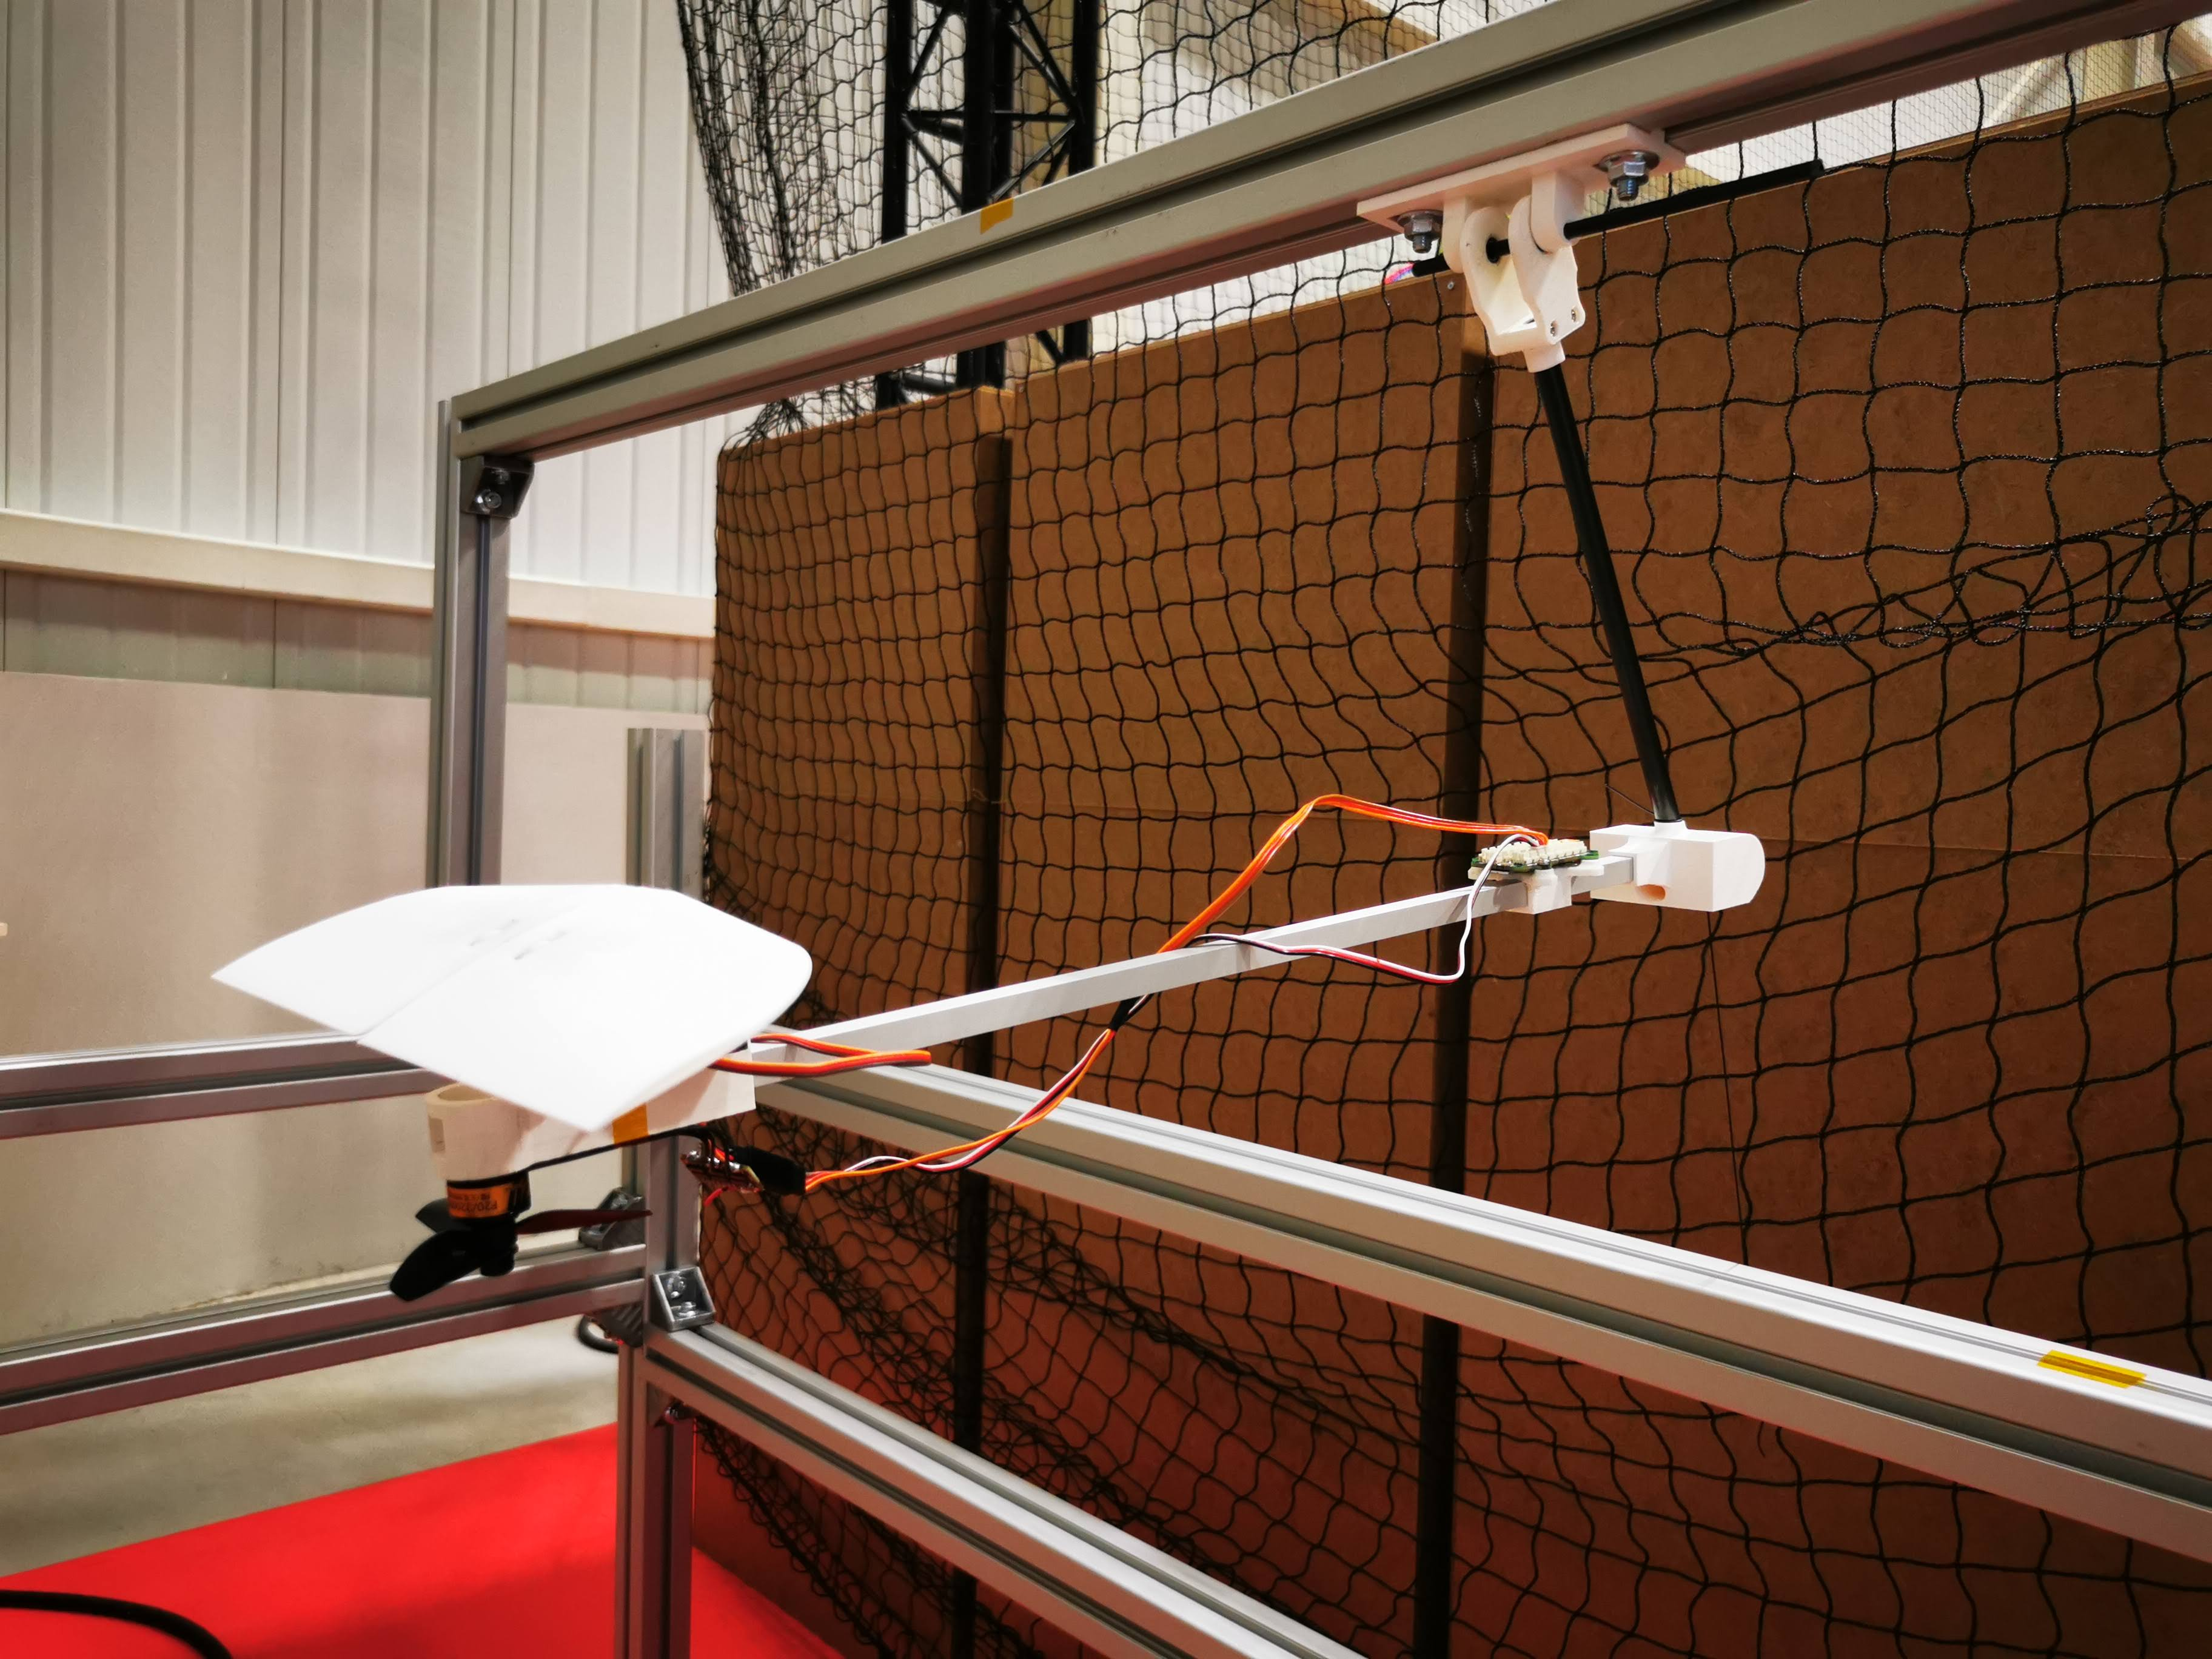
\includegraphics[trim={0 15cm 0 25cm},clip, width=0.7\columnwidth]{figures/IMG_20230120_141852.jpg}
    \caption{Maquette expérimentale du fuselage de Colibri.}
    \label{fig:colibri_fus}
\end{figure}
Le banc de test de la Figure \eqref{fig:colibri_fus} est un montage du fuselage sur un pivot fixe devant la soufflerie ouverte. Ce montage permet d'apprécier le fonctionnement de la commande \eqref{eq:pidfus} et son comportement face au vent.
}



\section{Expérimentations}
\label{sec:exp}
Un prototype a été mis au point, comme le montre la Figure~\ref{fig:colibri_real}. La Figure~\ref{fig:colibri_flight} présente une sélection des résultats expérimentaux en environnement contrôlé.


\begin{figure}[ht!]
    \centering
    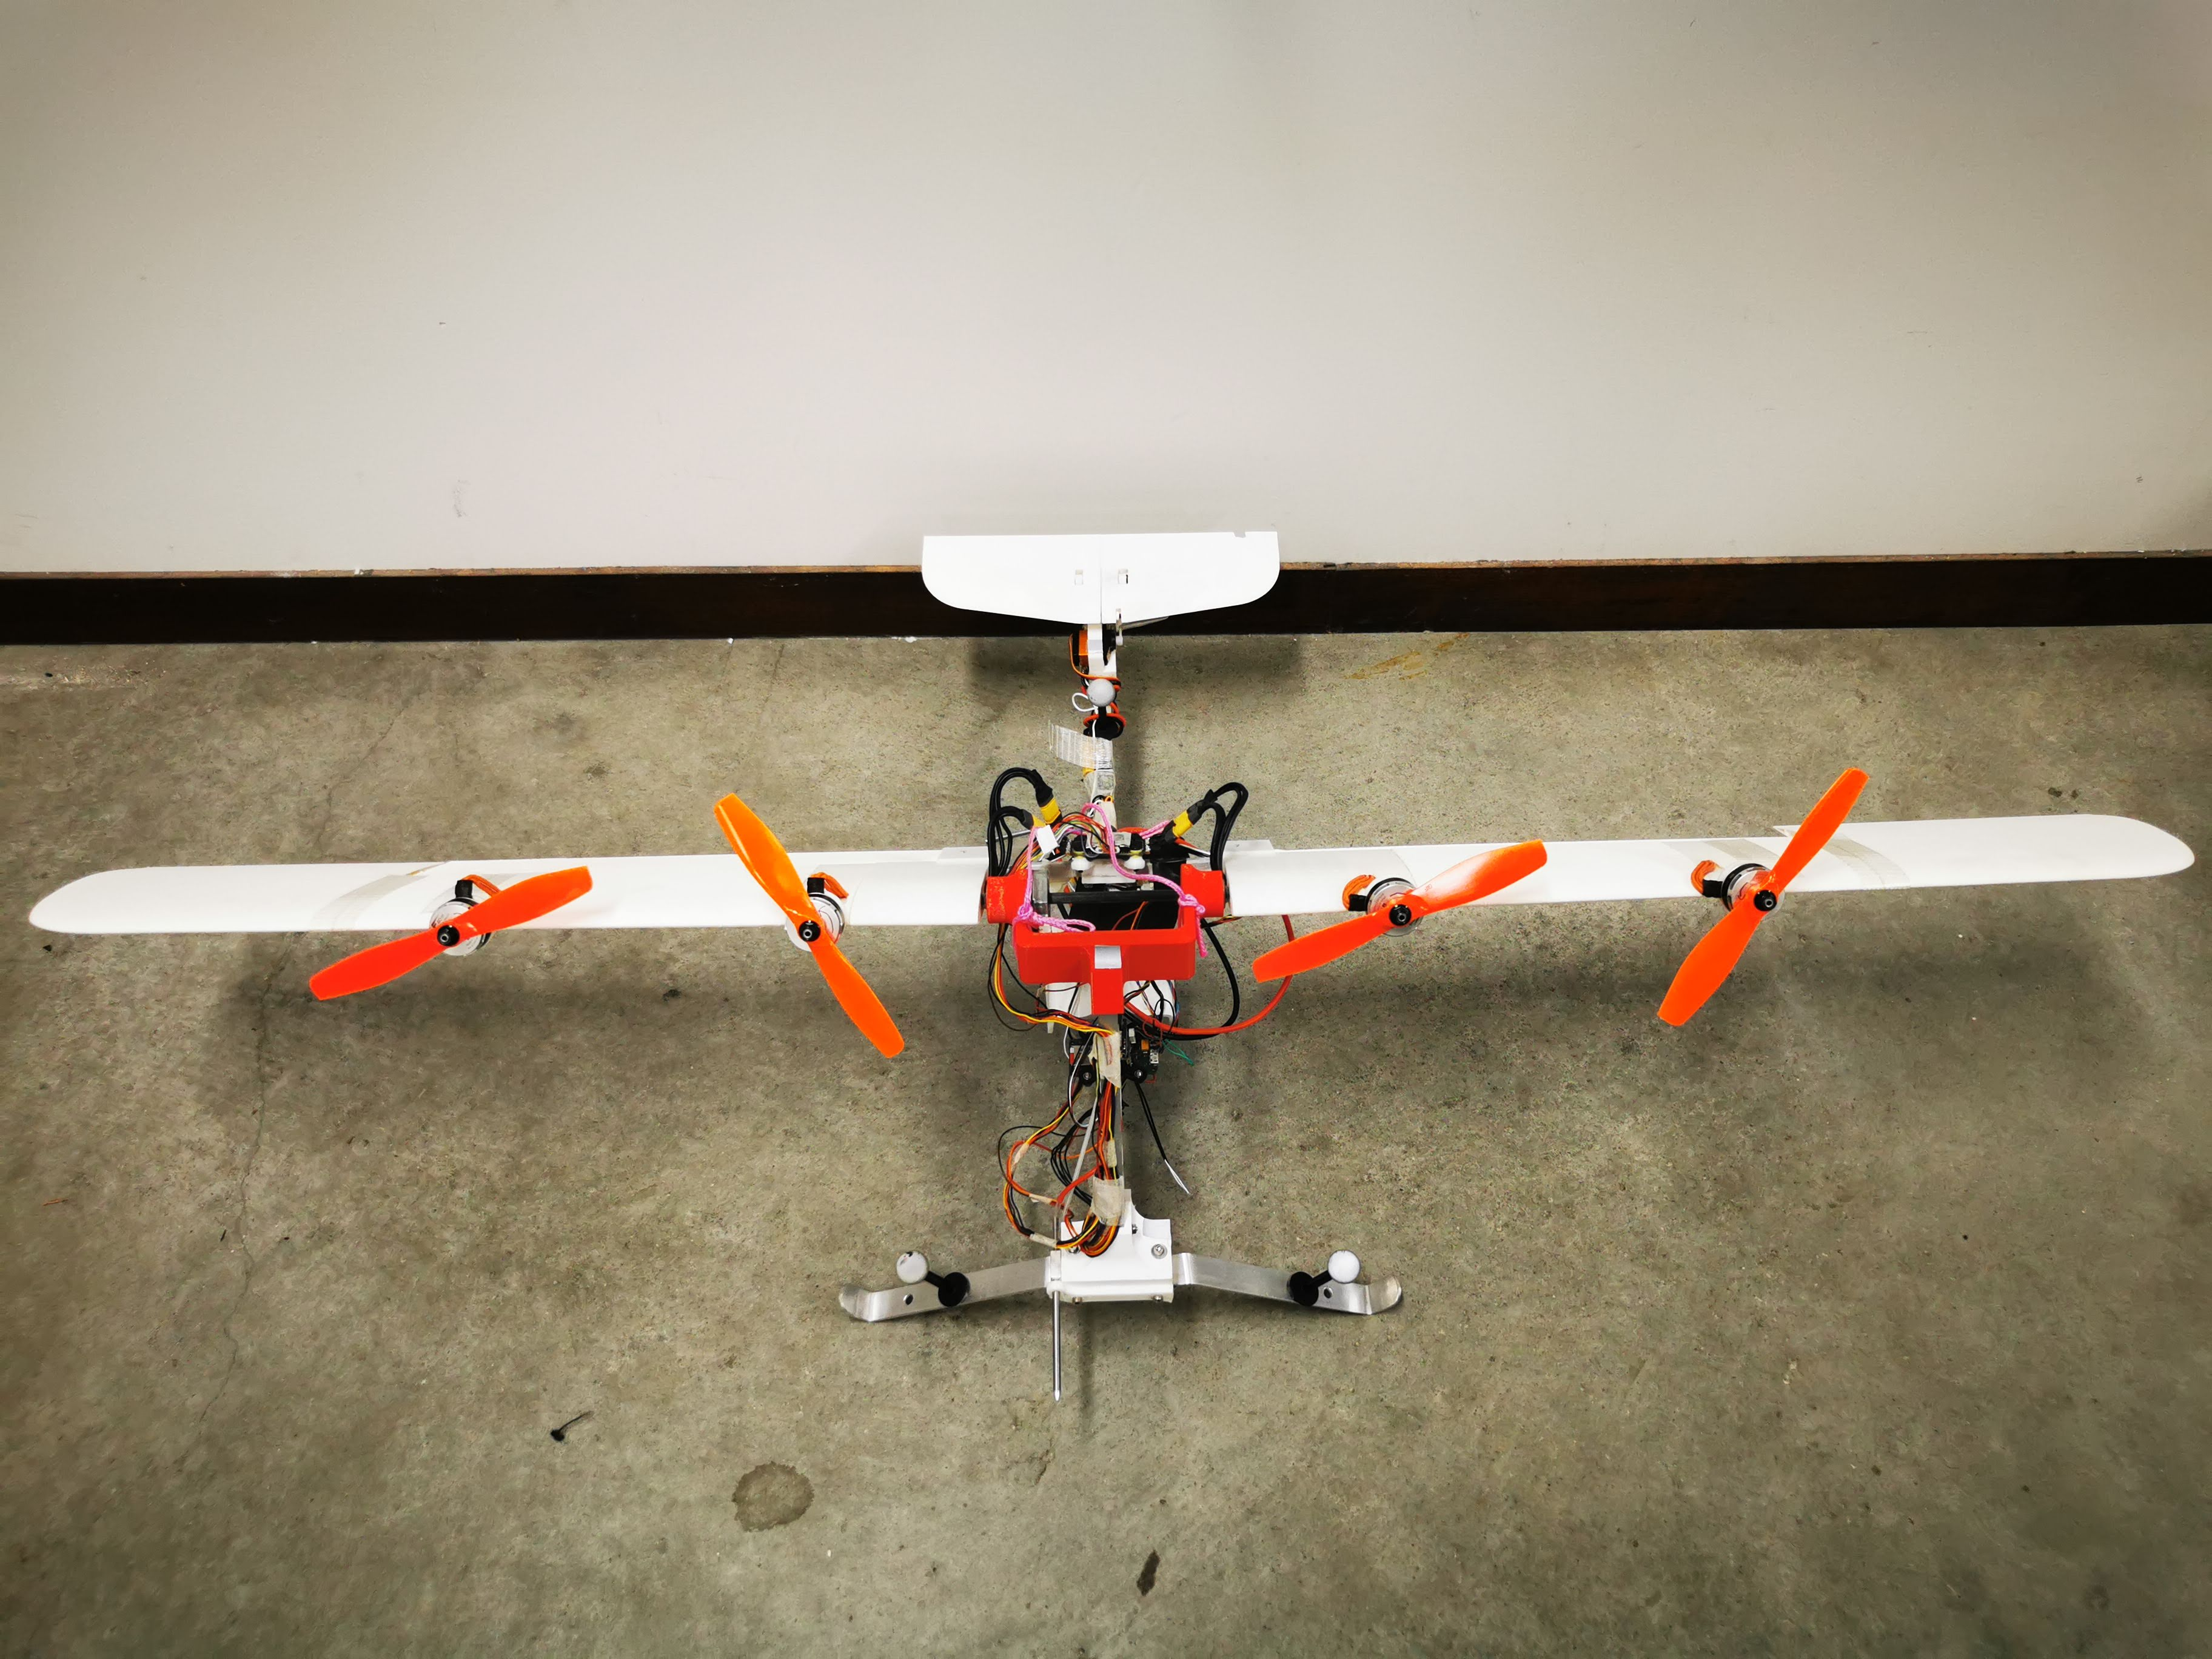
\includegraphics[trim={0 15cm 0 25cm},clip, width=0.6\columnwidth]{figures/colibri_real.jpg}
    \caption{Prototype : Colibri.}
    \label{fig:colibri_real}
\end{figure}

Sur la Figure~\ref{fig:colibri_flight}, de \SI{0}{\second} à \SI{8}{\second}, le drone est au sol. De \SI{8}{\second} à \SI{16}{\second}, le drone décolle pour atteindre une hauteur de 2 mètres, visible sur le troisième graphique. Cette hauteur est atteinte après un dépassement de 10 \%. Le drone est maintenu dans cette position pendant \SI{54}{\second}. Des oscillations d'incidence sont observées dans le cinquième et le dernier graphique, générant des oscillations dans la position horizontale du drone. Ce phénomène est dû au couplage entre les deux corps, qui n'est pas correctement stabilisé. À partir de \SI{70}{\second}, le drone commence à se diriger vers le point $\boldsymbol{p}_{c} = \begin{bmatrix} 3 & 0.9 & -1.5 \end{bmatrix}^\top$ et $\psi_{c}=\SI{90}{\degree}$.
\begin{figure}[ht!]
\centering
    \includegraphics[width=0.6\columnwidth,angle=0]{figures/colibri_flight.png}
    \caption{Position et orientation de l'aile (six premiers graphiques) et mesure de l'angle entre l'aile et le fuselage (dernier graphique), lors d'un vol réel. }
    \label{fig:colibri_flight}
\end{figure}
{\color{blue}

\section{Vol avec un contrôleur INDI unifié}
    Au vu du vol expérimental de la Figure~\ref{fig:colibri_flight}, nous avons supprimé le contrôleur proportionnel-dérivé du fuselage pour utiliser l'INDI. Nous ajoutons le moteur du fuselage comme actionneur dans le vecteur de commande $\boldsymbol{u}_{\text{W}}$ et nous ajoutons un nouvel objectif de stabilisation, lequel correspond à la stabilisation du fuselage $u_{\text{tail}}$.

    Ainsi, la matrice $\boldsymbol{G}$ définit dans \eqref{eq:INDI} devient : 
    \begin{align*}
        \begin{bmatrix}
        \partial \phi \\
        \partial \theta \\
        \partial \psi \\
        \partial T \\ 
        \partial \theta_{\text{F}}
        \end{bmatrix}\! =\! \boldsymbol{G} \boldsymbol{u}_{\text{W}} \!=\!
        \begin{bmatrix}
        -7.5 & -15 & 7.5 & 15 & 0 & 0 & 0\\
        0 & 0 & 0 & 0 & 15 & 15 & 0\\
        0 & 0 & 0 & 0 & 4 & -4 & 0 \\
        -0.6 & -0.6 & -0.6 & -0.6 & 0 & 0 & 0\\
        0 & 0 & 0 & 0 & 0 & 0 & 15 \\
        \end{bmatrix}
        \boldsymbol{u}_{\text{W}}.
    \end{align*}


    Dans le cas dynamique, le mouvement de l'aile et donc du point d'attache a un impact sur le fuselage. Il est donc nécessaire de réaliser une étude dynamique \eqref{eq:dynamiquependule}. Toutefois, en l'absence de vent, l'actionneur utilisé pour stabiliser le fuselage est le moteur qui ne peut générer qu'une force vers le bas (comme développé dans la section \ref{sec:stabfus}).
    \begin{remark}
        \label{rem:irréversibilité}
        En raison de l'irréversibilité de la génération de forces par le moteur du fuselage, une accélération positive ne pourra pas être contrebalancée par le moteur. Lors d'une décélération, une augmentation de la vitesse de rotation du moteur permet de compenser les accélérations linéaires et donc de maintenir le fuselage horizontal.
    \end{remark}

    Il est possible d'anticiper la commande de vitesse angulaire du fuselage en fonction des accélérations linéaires verticale $\ddot{z}$ et horizontale $\ddot{x}$ de l'aile.
    \begin{align}
        \label{eq:dynamiquependule}
        m l^{2} \ddot{\theta}_{\text{p}} + ml(g-\ddot{z}) \sin{\theta_{\text{p}}} + ml \ddot{x} \cos{\theta_{\text{p}}} = 0\\
        \implies \ddot{\theta}_{p} = -\frac{1}{l} \left( (g-\ddot{z})\sin{\theta_{\text{p}}} + \ddot{x} \cos{\theta_{\text{p}}} \right)
    \end{align}
    avec $l = \| \boldsymbol{d}_{\text{G}O_{\text{W}}} \|$ et $\theta_{\text{p}} = \theta_{\text{F}} - \frac{\pi}{2} - \arctan{\frac{{x}_{\text{G}O_{\text{W}}}}{{z}_{\text{G}O_{\text{W}}}}}$.
    En régime stationnaire, nous avons un équilibre qui assure que l'accélération de la gravité $g$ soit compensée par la traction de l'hélice $\boldsymbol{F}_{m}$. Nous discrétisons cette équation pour obtenir la commande \textit{feedforward} de vitesse angulaire : 
    \begin{align}
        \label{eq:feedforward}
        \dot{\theta}_{p} (t+1) = -\frac{1}{l} \left( (-\ddot{z})\sin{\theta_{\text{\text{p}}}} + \ddot{x} \cos{\theta_{\text{p}}} \right) + dot{\theta}_{\text{p}} (t).
    \end{align}
    De cette équation \eqref{eq:feedforward}, nous observons qu'il est possible de générer une trajectoire qui permette d'accélérer horizontalement sans générer un changement de vitesse angulaire du fuselage (qui ne pourrait pas être compensé voir remarque \ref{rem:irréversibilité}). Cette trajectoire utilise une accélération verticale $\ddot{z}$ pour assurer $ (-\ddot{z})\sin{\theta_{\text{p}}} + \ddot{x} \cos{\theta_{\text{p}}} = 0 $. Cette trajectoire est donc ascendante. Une autre solution à la remarque \ref{rem:irréversibilité} est de permettre la génération d'une force bidirectionnelle (en ajoutant un second moteur ou un servomoteur pour diriger la force).



}


\section{Vols expérimentaux}
\todo{Vols expérimentaux unifiés Photo volière}

\section{Conclusion}

Ce chapitre propose une nouvelle architecture de drone \textit{freewing} qui possède des caractéristiques intéressantes, tel qu'un fuselage maintenu horizontal pendant toutes les phases de vol, un décollage et un atterrissage vertical, et une passivité naturelle aux perturbations de vent. Toutefois, de nombreuses complexités apparaissent avec cette architecture. La modélisation multicorps menée a permis d'obtenir un modèle représentant le comportement du drone et une identification a isolé les coefficients pour que le modèle soit le plus réaliste. Un travail a été mené sur l'estimation de l'état d'un tel drone, permettant de conclure sur la meilleure position pour l'installation des capteurs et l'implémentation de la démarche nécessaire pour réaliser l'estimation de l'état. 

À l'aide de cette dernière, une stabilisation basée sur une double boucle INDI et proportionnelle dérivée a permis de réaliser une validation expérimentale de la maquette, de l'estimation de l'état. Toutefois, cette implémentation a montré les limites d'une architecture à deux boucles. Nous avons donc proposé une architecture de commande unifiée basée sur une rétroaction INDI, contrôlant les deux corps et permettant le contrôle expérimental d'un drone à fuselage pendulaire non actionné.








% \chapter{Commande d'un drone à aile libre rotation libre}
\minitoc

\section{Inversion non linéaire incrémentale de la dynamique du drone}

\section{Commande Udwadia-Kalaba}

\section{Vols expérimentaux}







% LTeX: enabled=true
\chapter*{Conclusion}
\addstarredchapter{Conclusion} 

\renewcommand{\thefigure}{C.\arabic{figure}}
\setcounter{figure}{0} % Réinitialiser le compteur à 0

\markboth{Conclusion}{Conclusion}
Cette thèse est consacrée à la modélisation, à l'étude et au contrôle d'un drone convertible sujet à des forces aérodynamiques, des couplages entre les actionneurs et des dynamiques non-linéaires. Elle propose, au travers de l'utilisation d'un modèle unifié représentant les forces aérodynamiques sur l'ensemble du domaine de vol, d'analyser le comportement d'un \textit{tailsitter} et de proposer des méthodes de commande. Notre travail a débouché sur la proposition d'une nouvelle architecture de type \textit{freewing}.

La première partie du manuscrit propose un rapide aperçu des architectures de drones convertibles avant de se focaliser sur les \textit{tailsitters} et les \textit{freewings}. Nous avons développé les principales caractéristiques d'actionnement, le comportement des drones ainsi que les méthodes de modélisation. Ce chapitre introductif a permis de développer l'architecture conventionnelle de commande, ainsi qu'un tour d'horizon des méthodes de commande et d'optimisation des contrôleurs. Notre travail ayant une forte composante expérimentale, une vision de l'architecture nécessaire à ces expérimentations a été évoquée avant d'être développée plus en profondeur dans l'Annexe.  

Nous avons utilisé un modèle de la littérature, sans singularité sur l'ensemble du domaine de vol, ne faisant pas appel aux angles aérodynamiques $\alpha$ et $\beta$, appelé $\phi$-théorie. Ce modèle mathématique n'a d'utilité pratique que s'il est cohérent avec la réalité, ce qui a pu être démontré dans la littérature et qui est confirmé par nos travaux. De ce modèle non-linéaire, nous avons pu extraire des caractéristiques intéressantes pour les drones à décollage et atterrissage vertical. 
Nous avons caractérisé l'ensemble des points d'équilibre avec ou sans vent pour un \textit{tailsitter}. De ces équilibres, nous avons extrait la dynamique linéarisée, point de départ de la conception de toute loi de commande linéaire. Notre compréhension du comportement du drone a été augmentée par ces résultats qui nous informent sur la commandabilité du drone, sur les marges vis-à-vis des saturations et sur la capture du comportement du drone par une linéarisation autour des points d'équilibre. Nous avons donc pu valider la précision des linéarisations face aux nombreuses non-linéarités du modèle. Pour cela, nous avons effectué des simulations en boucle fermée, au vu du comportement instable du drone, du modèle linéaire et non-linéaire.

Un travail préliminaire a permis de proposer une architecture de commande hybride avec un mécanisme d'hystérésis, basée sur une variable discrète sélectionnant la loi de commande la plus appropriée en fonction de la phase de vol. Les deux lois proposées dans ce cas sont une loi non-linéaire basée sur une direction de zéro-moment et une loi linéaire LQR. Cette loi LQR est optimisée grâce au modèle obtenu précédemment.

De ce travail et à l'aide de la linéarisation, nous avons observé un comportement intéressant pour le rejet de perturbations de vent sur un \textit{tailsitter}. Ce comportement repose sur le changement de l'angle de tangage du drone pour compenser l'augmentation de la vitesse air qui engendre un déplacement du drone. Nous avons donc expérimenté, à l'aide d'une maquette à trois degrés de liberté, une loi de commande proportionnelle intégrale. Cette maquette, utilisant une architecture physique associée à un modèle de dynamique transactionnelle simulée, a permis de valider l'architecture de commande ainsi que son optimisation basée sur des contraintes $H_{\infty}$.
Bien que les résultats obtenus soient prometteurs, nous avons étudié une méthode différente d'obtention des gains du contrôleur PI. Cette méthode, plus conservative, est basée sur une résolution successive de LMI. Les résultats ont pu être évalués sur l'architecture complète du drone, par un vol expérimental en volière.

Cette expérimentation a permis d'identifier des problèmes de sensibilité de la boucle fermée aux dynamiques non modélisées et aux bruits. Nous avons donc proposé une extension du contrôleur PI pour augmenter sa robustesse. Une expérimentation face à un vent croissant par palier a validé notre travail.

Nos travaux nous ont amené à vouloir installer un capteur de vent sur le drone pour pouvoir utiliser la mesure pour la transition. Toutefois, le corps du \textit{tailsitter} étant en rotation lors de la transition, nous ne pouvions pas fixer le capteur de manière satisfaisante. Nous avons donc étudié et développé une architecture \textit{freewing} procurant un fuselage maintenu horizontal permettant d'installer n'importe quel capteur ou charge utile. L'aile étant en rotation libre autour du fuselage, nous conservons de nombreuses propriétés des \textit{tailsitters}. Dans cette démarche, nous avons modélisé le drone avec une dynamique multicorps, identifié les paramètres, fabriqué la maquette et réalisé des vols expérimentaux à l'aide de l'INDI.

\section*{Limite de l'étude}
Les travaux préliminaires, menés au chapitre \ref{chap:hybrid}, ne sont que des résultats de simulation. Il serait souhaitable de réaliser des expérimentations du contrôleur non-linéaire basé sur une direction de zéro-moment ainsi que de son utilisation dans l'architecture hybride avec une transition entre le contrôleur basé sur une direction de zéro-moment et le contrôleur PI étendu développé au chapitre \ref{chap:6DOF}.

Bien que nous souhaitions utiliser la mesure du vent, notre travail n'a pu aboutir, étant donné la richesse des questions que nous avons souhaité développer en amont et par le temps nécessaire au développement de l'architecture nécessaire.
De plus, de nombreuses architectures auraient pu répondre au besoin. Nous avons choisi de nous concentrer sur une architecture inspirée du \textit{tailsitter} DarkO car nous avions de l'expérience dans sa modélisation et sa dynamique.

Tous nos résultats ont été expérimentés dans une atmosphère contrôlée avec un générateur de perturbations. Il serait maintenant intéressant d'évaluer la précision de nos contrôleurs en extérieur. Ce travail possède une double complexité car le drone évoluerait dans un environnement plus turbulent, mais aussi avec une estimation d'état moins précise. Effectivement, en intérieur, nous avons accès à un système de positionnement millimétrique alors qu'en extérieur, les GPS ne peuvent nous fournir une information de position aussi précise.


\section*{Travaux futurs}

La modélisation de Udwadia-Kalaba permet d'obtenir un modèle d'un drone multicorps. Il serait intéressant d'utiliser ces travaux pour concevoir un contrôleur assurant la stabilisation de l'aile et du fuselage en prenant en compte leurs interactions.

De plus, ce contrôleur pourrait profiter de la mesure du vent réalisée par une sonde cinq trous installée sur le fuselage. Comme le fuselage est maintenu horizontal et avec une faible variation d'incidence, la mesure sera disponible dans toutes les phases de vol. Il est nécessaire de caractériser la sonde. Effectivement, la mesure étant réalisée par une différence de pression statique et dynamique, nous devons donc étudier la sensibilité des capteurs pour déterminer la plus petite variation de vent mesurable ainsi que le temps nécessaire à la mesure.

Enfin, demeure un sujet de recherche, non abordé à ce jour : si les drones convertibles possèdent deux modes de déplacement (stationnaire et vol d'avancement), il conviendra de s'interroger sur la stratégie de vol à adopter, en fonction des caractéristiques de la mission.

En effet, en fonction de la distance entre deux points de l'espace, il s'agit de choisir entre :
\begin{itemize}
    \item effectuer une transition du mode stationnaire vers le mode d'avancement (plus efficace énergétiquement)
    \item ou rester en mode stationnaire et se déplacer de proche en proche (très énergivore).
\end{itemize}

Si le mode d'avancement est énergétiquement intéressant, il implique deux transitions et la réalisation d'un cercle (nécessaire pour de courtes distances et pour avoir le temps de réaliser les transitions).

Ce problème est schématisé sur la Figure \ref{fig:pbhybride}.



\begin{figure}[ht!]
    \centerline{
    \includegraphics[trim=0cm 0cm 0cm 0cm,clip,width=0.8\columnwidth]{figures/DroneConvertibleGuidage.png}}
    \caption{Schéma de déplacement d'un drone convertible.}
    \label{fig:pbhybride}
\end{figure}





%%%%%%%% 6. APPENDIX %%%%%%%%
\appendix

% LTeX: enabled=true
\chapter*{Annexe technique sur les drones}
\addstarredchapter{Annexe technique sur les drones} 

\markboth{Annexe technique sur les drones}{Annexe technique sur les drones}

\renewcommand{\thefigure}{A.\arabic{figure}}
\setcounter{figure}{0} % Réinitialiser le compteur à 0

\renewcommand{\thetable}{A.\arabic{table}}
\setcounter{table}{0} % Réinitialiser le compteur à 0

\section*{Système de drone : Paparazzi}

Un drone est composé de plusieurs pièces assemblées entre elles pour former la structure sur laquelle sont fixés des actionneurs, un autopilote et une charge utile (colis, caméra, capteur, etc.). L'élément central est l'autopilote qui assure la communication entre tous les éléments. Nous pouvons décomposer l'autopilote en deux parties : la partie matérielle et la partie logicielle.
\nomenclature[]{\(PCB\)}{Circuit imprimé  \textit{Printed Circuit Board}}
La partie matérielle est constituée d'un circuit imprimé (PCB) sur lequel des composants sont installés pour assurer les tâches relatives au vol. La partie logicielle se décompose en deux éléments : le segment sol et le logiciel embarqué.

Nous pouvons détailler les capteurs embarqués et le microcontrôleur avec l'ensemble de ses ports de communication. 

 \subsection*{Les capteurs d'un autopilote}
 Un autopilote comporte généralement un accéléromètre, un gyroscope, un magnétomètre et un baromètre.
 
 \paragraph*{}
 \textbf{L'accéléromètre} à trois axes permet de mesurer l'ensemble des forces appliquées sur le véhicule, à l'exception du poids. Il est possible d'obtenir la position du drone par double intégration de la mesure de l'accéléromètre. Toutefois, il convient de souligner que la position dérive rapidement en raison des bruits de mesure.

 \paragraph*{}
 \textbf{Le gyroscope} à trois axes permet de mesurer les vitesses de rotation du véhicule. Il est possible d'obtenir l'orientation du drone par intégration de la mesure du gyroscope. Toutefois, comme précédemment, l'orientation dérive rapidement en raison des bruits de mesure.

 \paragraph*{}
 \textbf{Le magnétomètre} à trois axes indique la direction du nord magnétique. Il permet de se diriger par rapport à une référence connue. Le principal inconvénient de ce capteur est sa perturbation par les masses magnétiques environnantes, ainsi que par les champs magnétiques parasites induits par la proximité des moteurs électriques par exemple. Il est donc difficile de les utiliser à l'intérieur d'un bâtiment. L'influence magnétique de l'engin porteur et les perturbations dues à d'éventuels moteurs électriques peuvent être éliminées en qualifiant, de manière statique, les erreurs dues aux masses métalliques du véhicule et aux moteurs électriques (en fonction des tensions et courants d'alimentation).

 \paragraph*{}

 \textbf{Le baromètre} est un capteur d'altitude basé sur la mesure de la pression atmosphérique. Cette pression est mesurée par un système électronique basé sur la résonance naturelle d'une pièce en alliage de nickel ou sur la modification de l'équilibre d'un pont de Wheatstone associé à un cristal de quartz sur lequel, par l'intermédiaire d'une capsule souple, s'exerce la pression atmosphérique. On déduit de la variation de pression atmosphérique une variation d'altitude à l'aide du modèle d'atmosphère standard qui nous indique qu'au niveau de la mer, la pression diminue de \SI{1}{\hecto\pascal} tous les \SI{8.5}{\meter}
 

 \paragraph*{}
 \textbf{Le GPS} est monté en extérieur de l'autopilote. Ce système de géopositionnement par satellite (\textit{Global Positioning System}) permet d'obtenir un positionnement absolu du drone. 

 \nomenclature[]{\(GPS\)}{Géo-positionnement par satellite (\textit{Global Positioning System})}
 \paragraph*{}
 Il est courant de retrouver plusieurs capteurs dans un même boitier, que l'on nomme centrale inertielle (Inertial Measurement Units, IMU). Ces dernières sont composées au minimum d'un accéléromètre 3-axes et d'un gyroscope 3-axes, mais il est courant de les trouver avec un magnétomètre 3-axes. 

 \nomenclature[]{\(IMU\)}{Centrales inertielles (\textit{Inertial Measurement Units})}

 \subsection*{Le microcontrôleur d'un autopilote}
 Le microcontrôleur (Microcontroller Unit, MCU) est la pièce maitresse de l'autopilote en ce qu'il permet d'effectuer l'ensemble des traitements nécessaires à la conduite du vol.

 \nomenclature[]{\(MCU\)}{Microcontrôleurs (\textit{Microcontroller Unit})}

 De plus, il possède plusieurs ports de communication pour récupérer les données des capteurs ou envoyer des ordres aux actionneurs.

La liaison série permet de relier deux équipements numériques pour qu'ils puissent s'échanger des informations. C'est le moyen de communication le plus simple. Toutefois, il contient un moyen de détection des erreurs tel que le bit de parité.

 Le protocole \textit{CAN} provient de l'industrie automobile. Il permet de raccorder à un même câble un grand nombre de calculateurs qui communiqueront donc à tour de rôle. Cette technique élimine le besoin de câbler des lignes dédiées pour chaque information à faire transiter (connexion point-à-point).

 Nous pouvons citer le \textit{Dshot} qui est un protocole de communication défini entre l'autopilote et l'ESC pour envoyer les commandes des moteurs. Les avancées sur ce protocole ont notamment permis la communication bidirectionnelle, permettant d'obtenir la vitesse des moteurs, leur consommation et d'autres informations.

 Enfin, le protocole \textit{I2C} est un bus de communication série simplifiant l'interconnexion de circuit intégré sur une même carte. Ce bus ne nécessite que deux fils pour être mis en place. Il n'est conçu que pour faire communiquer des équipements relativement proches (quelques centimètres).

 \subsection*{Évolutions}
 Les nombreux progrès dans les systèmes d'estimation état permettent de connaître précisément l'orientation et la position des drones pour assurer la stabilisation, le guidage et la navigation. Les progrès sont liés à l'amélioration continue des capteurs, notamment des centrales inertielles constituées d'un accéléromètre, d'un gyroscope et d'un magnétomètre.

La Table \ref{tab:autopilote_ev} montre l'évolution des vitesses des microcontrôleurs (Microcontroller Unit, MCU) \nomenclature[]{\(MCU\)}{Microcontrôleurs (\textit{Microcontroller Unit})} embarqués sur les autopilotes et de la réduction du bruit des capteurs inertiels.
\begin{table}[ht]
    \centering
    \begin{tabular}{|c|c|c|c|c|c|}
        \hline
        Type & Date & MCU & Vitesse & Capteur  & Bruit RMS \\
        \hline \hline
        \href{https://wiki.paparazziuav.org/wiki/Apogee/v1.00}{Apogee}  & 2013 & STM32F4 & 168 MHz & MPU-9150 & \begin{tabular}{ccc} Gyro : 0.06 dps \\
        Accel: 4 mg  \end{tabular}  \\
        \hline
        \href{https://wiki.paparazziuav.org/wiki/Chimera/v1.00}{Chimera} & 2016 & STM32F7 & 216 MHz &  MPU-9250 & \begin{tabular}{ccc} Gyro : 0.1  dps \\
        Accel: 8 mg  \end{tabular}\\
        \hline
        \href{https://wiki.paparazziuav.org/wiki/Tawaki/v1.10}{Tawaki 1} &2019 &  STM32F7 & 216 MHz  & ICM-20600 & \begin{tabular}{ccc} Gyro : 0.04 dps \\
        Accel: 1 mg  \end{tabular}\\
        \hline
        \href{https://wiki.paparazziuav.org/wiki/Tawaki/v2.01}{Tawaki 2} &2023 &  STM32H7 & 480 MHz & ICM-42688-P & \begin{tabular}{ccc} Gyro : 0.028 dps \\
        Accel: 0.70 mg  \end{tabular} \\
        \hline
    \end{tabular}
    \caption{Évolution des autopilotes Paparazzi sur dix ans.}
    \label{tab:autopilote_ev}
\end{table}

Sur une période de dix ans, nous pouvons observer que les microcontrôleurs ont doublé leur vitesse d'exécution, que les fabricants ont divisé par deux le bruit moyen sur les gyroscopes et par quatre le bruit moyen des accéléromètres.
Ces évolutions continues permettent une amélioration de l'estimation du drone utilisée pour la stabilisation. Il en résulte une stabilité accrue et de nouvelles possibilités pour la commande des drones.

 \subsection*{Les logiciels d'un autopilote}
 Tout le fonctionnement d'un drone repose sur le logiciel qui permet de le faire voler. Il se décompose en deux catégories : la partie sol et la partie embarquée.

 \subsection*{Le segment sol}

Le segment sol est un ensemble de logiciels permettant de monitorer l'état du drone et de lui envoyer des ordres. Il repose sur les informations échangées avec le drone au travers de la télémétrie. L'interface principale est la GCS \textit{Ground Control Station} (voir Figure \ref{fig:GCS}), laquelle assure la visualisation du drone sur la carte, ainsi que toutes les commandes nécessaires au vol (modification de point de passage, atterrissage, etc.). Elle est écrite en C++.

\begin{figure}[ht!]
    \centerline{
    \includegraphics[trim=0cm 0cm 0cm 0cm,clip,width=0.8\columnwidth]{figures/GCS.png}}
    \caption{Interface graphique de la station de contrôle au sol.}
    \label{fig:GCS}
\end{figure}

\nomenclature[]{\(GCS\)}{Station de contrôle au sol \textit{Ground Control Station}}

Une autre partie du segment sol est le code serveur qui gère les messages échangés entre les différentes applications. Le code est en Ocaml.

Enfin, un code assure la compilation croisée du logiciel embarqué qui doit être téléversé sur le drone, basée sur des Makefile et du code Ocaml. Le logiciel embarqué est décrit par la suite.

 \subsection*{Le logiciel embarqué}
 Le logiciel embarqué est un code écrit en C, intégré dans un système d'exploitation temps réel "Chibios". Il est téléversé sur le microcontrôleur au travers d'une sonde de programmation ou de la prise USB présente sur l'autopilote.

 L'ensemble du code est organisé sous la forme de modules que l'on change au besoin. Chaque module assure des fonctionnalités telles que l'estimation d'état, la stabilisation, le guidage, la navigation ou encore la gestion de la charge utile (voir Figure \ref{fig:schedulingpaparazzi}). Grâce à un mécanisme de gestion de dépendance, les modules ont la possibilité de charger d'autres modules nécessaires à leur fonctionnement. L'ordre de compilation et d'édition des liens seront gérés par le logiciel de compilation.


 \begin{figure}[ht!]
    \centerline{
    \includegraphics[trim=0cm 0cm 0cm 0cm,clip,width=0.7\columnwidth]{figures/PPRZ_Main_ap_loop.png}}
    \caption{Schéma de l'ordre d'exécution des codes embarqués \cite{RTDpaparazzi2022}.}
    \label{fig:schedulingpaparazzi}
\end{figure}

 
\section*{AM32}
Le logiciel AM32 est conçu pour les microprocesseurs ARM STM32 afin de contrôler un moteur \textit{brushless}, couramment utilisé pour les drones. Le logiciel est conçu pour être sûr et rapide, avec des démarrages rapides et sans à-coups et une accélération linéaire. Il est destiné à être utilisé avec plusieurs types de véhicules et de contrôleurs de vol. 

L'intérêt de ce logiciel est qu'il est ouvert, permettant de contribuer, en proposant des évolutions. Nous avons ainsi implémenté l'approche de \cite{franchi2017}, avec un algorithme de biais et de gain adaptatif (ABAG) (voir \ref{fig:ABAG_algo}).

\begin{figure}[ht!]
    \centerline{
    \includegraphics[trim=0cm 0cm 0cm 0cm,clip,width=0.6\columnwidth]{figures/ABAG_algo.png}}
    \caption{Algorithme de biais et de gain adaptatif (ABAG) \cite{franchi2017}.}
    \label{fig:ABAG_algo}
\end{figure}
L'algorithme ABAG est adaptatif et robuste en ce qu'il ne nécessite pas la connaissance des paramètres mécaniques ou électriques du groupe moteur et hélice et qu'il n'est pas nécessaire de procéder à une identification, ni de connaître l'entrée nominale. De plus, l'algorithme ABAG ne nécessite que très peu de ressources de calcul, ce qui en fait un atout important pour un système embarqué.

 % Revenir à la numérotation normale après la section si nécessaire
\renewcommand{\thefigure}{\thechapter.\arabic{figure}}
\renewcommand{\thetable}{\thechapter.\arabic{table}}

%%%%%%%% 7. BIBLIOGRAPHIE %%%%%%%%
\bibliographystyle{StyleThese}
% \bibliographystyle{plain}
\bibliography{biblio}


%%%%%%%% 8. LAST PAGE %%%%%%%%
\cleardoublepage
\pagestyle{empty} % remove headers on 2e page
\newgeometry{left=1.5in,right=1.3in,top=1.1in,bottom=1.1in} % remove header/footer space

% French
\begin{vcenterpage} % note: vcenterpage is not needed for long abstrat
\noindent\rule[2pt]{\textwidth}{0.5pt}

{\large\textbf{Résumé :}}
Les drones sont aujourd'hui devenus un outil dans de nombreux domaines tels que l'inspection, la surveillance ou la maintenance. Cependant, ils souffrent d'une autonomie limitée. Les \textit{tailsitters} apportent une solution grâce à leur grande enveloppe de vol et à leur efficacité énergétique. Toutefois, les \textit{tailsitters} sont grandement sujets aux perturbations aérologiques et notamment aux turbulences dans les phases stationnaires principalement. Cela est dû à la grande surface d'aile verticale, laquelle possède une grande prise au vent. De plus, leur corps tournant lors de la transition, il est donc compliqué de mesurer la vitesse de l'air.  Ainsi, en stationnaire ou à faible vitesse, le vent n'est pas connu. Ce type de drone est sous-actionné puisque l'on trouve deux moteurs sur l'aile et deux surfaces aérodynamiques sur le bord de fuite. Le flux d'air des hélices soufflant les élevons, nous avons un couplage entre les actionneurs.

Cette thèse cherche à étudier la commande de drones dans des environnements perturbés ou en présence de vent. Les premiers travaux se sont concentrés sur la dynamique sans vent pour appréhender une dynamique simplifiée. Nous avons pu proposer une modification non-linéaire du vecteur de commande pour rendre ce modèle linéaire en commande. De ce modèle, nous avons proposé une loi de commande locale-globale fondée sur une dynamique hybride à hystérésis. Elle permet d'étendre le domaine de stabilité de la loi de commande linéaire agressive à l'aide d'une loi non-linéaire avec une grande région d'attraction, mais moins agressive.

La suite des travaux s'est concentrée sur la stabilisation d'un \textit{tailsitters} soumis à des échelons de vent. Il en résulte une caractérisation des équilibres stationnaires pour un ensemble de conditions de vent et l'obtention de la représentation linéarisée de la dynamique du drone. À l'aide de ce modèle, il a été possible d'analyser les saturations des actionneurs et l'autorité disponible aux environs des points d'équilibre. Nous avons réalisé une stabilisation établie sur un retour de sortie, avec une action proportionnelle et intégrale. Cette commande n'utilise pas la mesure de l'angle de tangage du drone, car nous ne pouvons pas, a priori, connaître la valeur cible qui nécessiterait une estimation de la vitesse et de la direction du vent. L'optimisation de ce bouclage est effectuée à l'aide du logiciel "Systune" pour obtenir de bonnes propriétés de réjection de perturbation. Une approche incrémentale a été suivie, la loi de commande ayant été testée dans un premier temps sur une maquette à un degré de liberté face à une soufflerie ouverte. Une fois validée, la loi de commande a été implémentée dans le système de drone Paparazzi. Grâce à son architecture modulaire, il a été possible de nous interfacer avec les codes d'estimation et de commande des actionneurs. Ainsi, nous avons pu réaliser des vols sur le modèle complet à six degrés de liberté.

Enfin, nous avons proposé une architecture inspirée du \textit{tailsitter}, nommée \textit{freewing}. Nous avons développé un drone multicorps basé sur une aile en rotation libre sur son axe de tangage autour d'un fuselage. L'actionnement de l'aile est sensiblement le même que pour le \textit{tailsitters} et le fuselage possède deux actionneurs pour se maintenir horizontal. Nous recherchons, dans cette architecture, une passivité naturelle à la turbulence induite par le changement naturel de l'incidence de l'aile en fonction du vent incident. Il s'agit aussi d'installer une charge utile sur le fuselage horizontal sur le domaine de vol. De plus, nous avons réalisé un modèle de simulation où la dynamique est obtenue à l'aide des équations de Udwadia-Kalaba et de la phi-théorie. Enfin, nous nous sommes concentrés sur la stabilisation et le guidage du drone en utilisant une inversion incrémentale non-linéaire de la dynamique (INDI). Nous utilisons les actionneurs de l'aile et du fuselage pour obtenir une loi de stabilisation globale. Des vols ont validé l'intérêt de cette architecture.

{\large\textbf{Mots clés :}}
mots, clefs
\todo{Mots clés}

\noindent\rule[2pt]{\textwidth}{0.5pt}
\end{vcenterpage}

% English
\newpage
\begin{vcenterpage}
\noindent\rule[2pt]{\textwidth}{0.5pt}
% LTeX: language=en
{\large\textbf{Abstract:}}
Drones have become a prevalent tool in numerous fields, including inspection, surveillance, and maintenance. However, one area where they are currently lacking is autonomy. Tailsitter offer a viable solution, combining large flight envelopes with energy efficiency. Nonetheless, tailsitter unmanned aerial vehicles are particularly susceptible to disturbances, specifically turbulence during hover phases. This is because of the large vertical surface area of the wing, which offers a high degree of wind resistance. Furthermore, the drone's body rotates during transition, making it difficult to accurately measure airspeed. It is not possible to accurately measure wind speed, whether the drone is hovering or moving at a low speed. Additionally, this underactuated drone, has two motors on the wing and two aerodynamic surfaces on the trailing edge. The interaction of the airflow from the propellers with the elevons results in a coupling between the actuators.

The aim of this thesis is to examine the control of drone in challenging environments, with a particular emphasis on the impact of wind. However, initial research focused on windless dynamics in order to gain a better understanding of the simplified dynamics. We were able to propose a non-linear modification of the control vector to transform this nonlinear model into an input-affine model. Based on this model, we proposed a local-global control law based on hybrid dynamics with hysteresis, which allowed us to extend the stability domain of an aggressive linear control law by means of a non-linear law with a large region of attraction, but which was less aggressive. 

Further work was conducted on the stabilization of a tailsitter drone under wind steps. This resulted in a characterization of stationary equilibria for a range of wind conditions and a linearized representation of the drone's dynamics. Using this model, we were able to analyze the saturation levels of actuators and the authority available close to the equilibrium points. We have implemented a stabilization system based on output feedback with proportional and integral action, derived from the model. This control does not utilize the drones pitch angle measurement, since the target value is not known a priori. It would require an estimation of wind speed and direction, which is not feasible. The loop is optimized using "Systune" software in order to achieve effective disturbance rejection properties. We adopted an incremental approach by initially evaluating the control law on a one-degree-of-freedom model against an open wind tunnel. Upon validation, we proceeded to implement the control law within the Paparazzi UAV system. Due to its modular design, we were able to establish a connection with the state estimation and actuators, enabling us to execute flights on the entire model with six degrees of freedom. 

We then proposed an architecture inspired by the tailsitter, called freewing. We have developed a multi-body drone that is based on a wing that can freely rotate on its pitch axis around a fuselage. The wing is driven the same way as the tailsitter, and the fuselage has a motor and an aerodynamic surface to keep it horizontal. With this architecture, we aim to achieve a natural passivity to turbulence induced by the natural change in wing incidence as a function of the incident wind. However, there is also the possibility of installing a payload on the horizontal fuselage. To obtain a simulation model, we have modeled the drone's dynamics using the Udwadia-Kalaba equations and the phi-theory. We focused on stabilization and guidance of the UAV through the use of incremental nonlinear dynamic inversion (INDI). The wing and fuselage actuators are used to achieve a global stabilization law. In order to evaluate the benefits of this architecture, we conducted flight tests.

{\large\textbf{Keywords:}}
key, words
\todo{Keywords}

\noindent\rule[2pt]{\textwidth}{0.5pt}
\end{vcenterpage}


\end{document}
